%% LyX 2.3.3 created this file.  For more info, see http://www.lyx.org/.
%% Do not edit unless you really know what you are doing.
\documentclass[12pt,oneside,norsk]{book}
\renewcommand{\rmdefault}{cmr}
\renewcommand{\sfdefault}{cmss}
\renewcommand{\ttdefault}{cmtt}
\renewcommand{\familydefault}{\rmdefault}
\usepackage[LGR,T1]{fontenc}
\usepackage[latin9]{inputenc}
\usepackage[a4paper]{geometry}
\geometry{verbose,tmargin=2cm,bmargin=2cm,lmargin=2cm,rmargin=2cm,headheight=1cm,headsep=1cm,footskip=1cm}
\setcounter{secnumdepth}{3}
\setcounter{tocdepth}{3}
\setlength{\parskip}{\medskipamount}
\setlength{\parindent}{0pt}
\usepackage{color}
\usepackage{babel}
\usepackage{array}
\usepackage{longtable}
\usepackage{float}
\usepackage{textcomp}
\usepackage{url}
\usepackage{pdfpages}
\usepackage{slashed}
\usepackage{multirow}
\usepackage{amsmath}
\usepackage{graphicx}
\usepackage[unicode=true,pdfusetitle,
 bookmarks=true,bookmarksnumbered=true,bookmarksopen=false,
 breaklinks=false,pdfborder={0 0 1},backref=page,colorlinks=false]
 {hyperref}

\makeatletter

%%%%%%%%%%%%%%%%%%%%%%%%%%%%%% LyX specific LaTeX commands.
\DeclareRobustCommand{\greektext}{%
  \fontencoding{LGR}\selectfont\def\encodingdefault{LGR}}
\DeclareRobustCommand{\textgreek}[1]{\leavevmode{\greektext #1}}
\ProvideTextCommand{\~}{LGR}[1]{\char126#1}

%% Because html converters don't know tabularnewline
\providecommand{\tabularnewline}{\\}
%% A simple dot to overcome graphicx limitations
\newcommand{\lyxdot}{.}


%%%%%%%%%%%%%%%%%%%%%%%%%%%%%% Textclass specific LaTeX commands.
\newenvironment{lyxlist}[1]
	{\begin{list}{}
		{\settowidth{\labelwidth}{#1}
		 \setlength{\leftmargin}{\labelwidth}
		 \addtolength{\leftmargin}{\labelsep}
		 \renewcommand{\makelabel}[1]{##1\hfil}}}
	{\end{list}}

\@ifundefined{date}{}{\date{}}
\makeatother

\usepackage{listings}
\renewcommand{\lstlistingname}{«Listing»}

\begin{document}
\title{Undervisningsnotater Automatiseringssystemer 2019 - 3AUA Gand VGS}

\maketitle
\tableofcontents{}

\chapter{Fremdriftplaner}

\section{Plan IO Treningsbrett\label{sec:Gand-RIO-Trainer} Uke 34-39}

\begin{longtable}[c]{|>{\centering}p{0.75cm}|>{\raggedright}p{3cm}|>{\raggedright}p{4cm}|>{\raggedright}p{4cm}|c|>{\centering}p{2cm}|}
\hline 
Uke & Emne & Kompetansemål & Læremål  & Tid & Link\tabularnewline
\hline 
\endhead
\hline 
34 & Releer, kontaktorer og posisjonsfølere &  & Releer og kontaktorer

Posisjonsfølere (mekaniske brytere og nærhetsfølere)

Enkoder & 6 & \href{https://www.nb.no/items/0be26fb9e7db598bef01cd2ca564e140?page=200&searchText=ellef\%20wahlstr\%C3\%B8m}{Teori}

\href{https://www.nb.no/items/323cdc70aad01a4ff184b78184f41eb7?page=22&searchText=ellef\%20wahlstr\%C3\%B8m}{Oppgaver}\tabularnewline
\hline 
34 & Installasjon av programvare &  & Kunne installere aktuelle programmer på egen PC

PCSchematic

Codesys & 4  & \tabularnewline
\hline 
34 & Tegning av motorstyring &  & Kunne laget tegninger i PC|Schematic. Fokus på

Kabel, rekkeklemmer & 2 & \href{http://www.pcschematic.com/Download/ELautomation/Manuals/DK/DK_Tutorial_Motorstyring.pdf}{Tutorial Motorstyring}\tabularnewline
\hline 
34 & HMI - Innføring &  & Kunne sette inn ferdige symboler og koble disse mot variabler

Bruke fargestandard fra HPHMI.  & 2 & \ref{subsec:Introduksjon-til-High}\tabularnewline
\hline 
34-35 & Programmering av kominatoriske styringer &  & Kunne løse kombinatoriske styringsoppgaver.  & 10 & \ref{subsec:Kombinatorsike-styringer}\tabularnewline
\hline 
 &  &  &  &  & \tabularnewline
\hline 
35 & IO Treningsbrett &  & Kunne måle opp, montere utstyr og forklare virkemåten til alt utstyret.

Kunne tegne arrangementstegning & 2 & \tabularnewline
\hline 
 &  &  &  &  & \tabularnewline
\hline 
35-36 & Codesys &  & Kunne koble opp mot ulike PLS-er og legge inn et program.  & 2 & \ref{subsec:Introduksjon-til-CoDeSys}\tabularnewline
\hline 
36 & RS-485 med modbus &  & Sette opp serie kommunikkasjon mellom to enheter

Kunne installere og sette opp kommunikasjon mellom to RS-485 modbus
enheter.

Kunne hente og skrive til dataregister ved hjelp av modbus.  & 2 & \ref{subsec:RS232}\tabularnewline
\hline 
 &  &  &  &  & \tabularnewline
\hline 
35-36 & Tegning av PLS styringer &  & Kunne tegne PLS styinger 

Referansesymbol og koblingssymbol & 2 & \href{http://www.pcschematic.com/Download/ELautomation/Manuals/DK/DK_Tutorial_Plc.pdf}{Tutorial PLS styring }\tabularnewline
\hline 
 &  &  &  &  & \tabularnewline
\hline 
35 & Styresignaler & -Diskrere PNP/NPN 

-Strømsløyfe 

-Analoge IO &  & 6 & \ref{sec:Styresignaler}\tabularnewline
\hline 
 &  &  &  &  & \tabularnewline
\hline 
37 & Motorstyring & vurdere hvilke regelverk og normer som gjelder for arbeidet som skal
utføres og anvende dette

bruke gjeldende regelverk og normer for elektriske installasjoner
på maskiner & Kunne beskrive virkemåte for asynkronmotoren

Kunne beskrive startmetoder for asynkronmotoren

Kunne beskrive driftsegenskaper ved asynkronmotoren

Kunne beskrive krav til en motorinstallasjon & 4 & \href{https://www.nb.no/items/0be26fb9e7db598bef01cd2ca564e140?page=77&searchText=ellef\%20wahlstr\%C3\%B8m}{Obligatorisk lesestoff s 76-89}

\href{https://www.nb.no/items/323cdc70aad01a4ff184b78184f41eb7?page=11&searchText=ellef\%20wahlstr\%C3\%B8m}{Gjør oppgaver side 11 og 12}\tabularnewline
\hline 
34 & Sikkerhetsrelatertedeler av styresystemet &  & Kunne beskrive hva som menes med en sikkerhetsrelatert styrefunksjon

Forklare hvorvor vi koble ene siden av styrekretser til PE. 

Kunne forklare hvorfor vi benytter skjermet kabel koblet til PE. 

Forklare funksjonen til Start (restart) i styrekretser

Kjenne til kravene for nødstopp & 4 & \ref{subsec:Sikkerhetsrele-og-sikkerhetsrela}\tabularnewline
\hline 
 & Trykk  &  &  & 8 & \tabularnewline
\hline 
 & Gandsfjorden Gondolbane &  & Arbeidsoppddrag med oppkobling av simulert Gondolbane & 16 & \tabularnewline
\hline 
\end{longtable}

\subsection{Innledning}

Gand RIO-Trainer er et treningskort for:
\begin{itemize}
\item oppkobling mot modbus RTU enheter
\item tilkobling av inngangssignaler til en PLS analoge (0-20mA og 0-5V)
og 0V/24V signaler
\item tilkobling av open collector utgangssignaler
\item PWM signal
\end{itemize}
Kortet kobles til PLS med en USB kabel og en trenger en USB til seriel
driver (CH340). 

\includegraphics[width=1\textwidth,bb = 0 0 200 100, draft, type=eps]{Gand RIO-Trainer.jpg}

\begin{tabular}{|c|c|c|c|}
\hline 
\multicolumn{4}{|c}{}\tabularnewline
\hline 
\hline 
IO & Tilkobling & Modbus registers Register  (Hex) & \tabularnewline
\hline 
Encoder &  & 0000 & Enkoder telleverdi\tabularnewline
\hline 
DO1 & åpen kollektor & 0001 & bit0\tabularnewline
\hline 
DO2 & åpen kollektor & 0001 & bit1\tabularnewline
\hline 
DO3 & åpen kollektor & 0001 & bit2\tabularnewline
\hline 
DO4 & åpen kollektor & 0001 & bit3\tabularnewline
\hline 
PWM1 & åpen kollektor & 0002 & AO 0 (PWM)\tabularnewline
\hline 
PWM2 & åpen kollektor & 0003 & AO 1 (PWM)\tabularnewline
\hline 
PWM3 & åpen kollektor & 0004 & AO 2 (PWM)\tabularnewline
\hline 
DI1 & 24VDC & 0005 & bit0\tabularnewline
\hline 
DI2 & 24VDC & 0005 & bit1\tabularnewline
\hline 
DI3 & 24VDC & 0005 & bit2\tabularnewline
\hline 
DI4 & 24VDC & 0005 & bit3\tabularnewline
\hline 
DI5 & 24VDC & 0005 & bit4\tabularnewline
\hline 
DI6 & 24VDC & 0005 & bit5\tabularnewline
\hline 
AI1 & 4-24mA/0-5V & 0006 & AI6\tabularnewline
\hline 
AI2 & 4-24mA/0-5V & 0007 & AI1\tabularnewline
\hline 
\end{tabular}

\subsubsection{Oppgaver til Gand RIO Trainer}
\begin{enumerate}
\item Lag et test program for å teste alle funksjonene på kortet
\item Koble til to ulike typer givere til en DI inngang
\item Koble til en analog transmitter med 4-20mA utgang til AI
\item Lag en kobling som der du kan styre en kontaktor med DO1
\end{enumerate}

\subsection{Arbeidsoppdrag Gondolbane over Gandsfjorden}

Dette er det første arbeidsoppdraget på VG3 Automasjon. Målet med
oppdraget er at dere skal få repitert mye av det dere kan fra VG2
samt å bli kjent med utstyr og software vi bruker på VG3 Automajon. 

Typisk nye ting du må lære det er:
\begin{itemize}
\item PLS programeringsverktøyet Codesys
\item Koblinger på Gand PLS og Gand RIO-Trainer
\end{itemize}
Fokus for repitisjon:
\begin{itemize}
\item Skjemategning
\item Regler og forskrifter
\item Givere
\item Programmering av Kombinatorisk styring. 
\item Nødstopp og sikkerhetsrelaterte deler av styresystemet
\item Asynkronmotoren
\item Motorstartere
\end{itemize}
I oppdraget skal du koble opp en simulert styring av en Gondol bane
over Gandsfjorden. Oppdraget består av følgende:
\begin{itemize}
\item Tegning av nødvendige elektriske kretser h.h.t regelverk og krav fra
kunde (lærer) PS. regelverk har forrang forran lærer. 
\item Bestilling av nødvendig utstyr
\item montering av utstyr
\item programmering av maskinen
\item Verifikasjon av:
\begin{itemize}
\item Koblinger
\item Sikkerhet
\item Funksjon
\end{itemize}
\end{itemize}
\includegraphics[width=1\textwidth,bb = 0 0 200 100, draft, type=eps]{Gondol.png}

Koble opp brettet i

Virkemåten til anlegget skal være som følger:

Sikkerhetsrelaterte deler av styringen:

Klar lys/knapp: For å gjøre gondolen klar for start trykkes klar knappen
og en vil få et klar lys(grønt) om sikkerhetsrelaterte deler av styresysteme
er ok. 

Vanlig styring:

Normal start: Når gondol står i stopp posisjon, startes den med startknapp
og går til andre side. 

Start midt på: gondol kjøres manuelt i ønsket retning, ved å holde
startknapp inne i 5 sek. går gondolen av seg selv. 

Alarm: Glidelager med trykkovervåkning. Range for trykkmåler er 0-1
bar. Om trykket synker under 0.7 bar. genereres en alam med blinkende
lys. når en trykker på lyd/knappen lyser det konstant. Alarmen resettes
når trykket overstiger 0.9bar. 

Manuell kjøring: For å få gondolen i service posisjon skal det være
mulig å kjøre manuelt i begge retninger. Når en kommer til service
posisjon skal en ikke kunne kjøre lengre manuelt.

Sikkerhetsrelatere deler av styresystemet.

Består av en nødstopp kanpp og to endebrytere. 


\subsubsection{Fremdriftsplan}

En typisk fremdrifsplan bør minst ha følgende punkter i rekkefølge
\begin{enumerate}
\item Tegne skjemategninger
\item Lage IO-liste
\item Starte PLS programmering Opplasting av PLS program
\item Koblingsarbeid
\begin{enumerate}
\item Risikovurdering av arbeidet
\item Montere utstyr
\item Merke utstyr
\item Koble utstyr i skap
\item Legge kabler
\item Koble Kabler
\item IO-Sjekk
\end{enumerate}
\item Verifikasjon også kalt sluttkontroll (det må settes opp sjekklister
for alt som skal kontrolleres under verifikasjon)
\begin{enumerate}
\item Sjekk anlegg mot dokumentasjon
\item Kontinuitet av PE
\item Isolasjonsmåling (IKKE LOV PÅ IOBRETT!!!!!!!!!!!!!!!!!!!!!!!!!!!!!!!!!!)
\item Sjekk av funksjon
\end{enumerate}
\end{enumerate}

\subsubsection{Oppkobling }

\subsubsection{IO-sjekk }

\subsubsection{Kalibrering og justering av DP-celle for 0-1 bar}

\paragraph{Planlegging}

Bør inneholde HMS, FSE , med risikovurdering av selve arbeidet

Fremdriftsplan som en punktvis liste over hva arbeidet kommer til
å bestå av. 
\begin{enumerate}
\item Samle og klargjør nødvendig utstyr, prossedyrer og dokumentasjon
\item Ta på personlig verneutstyr
\item Transport til arbeidssted (kan være bare å gå, men kan også være at
du må kjøre, bruke stillas, lift o.l.)
\item På arbeidssted sjekk TAG for å sikre at korret utstyr er funnet.
\item Utførelsen av selve arbeidet. 
\item Opprydding og klargjøring av arbeidssted og tilbakestilling av utstyr. 
\item Dokumentasjon beskrivelse av hva som skal dokumenteres. (arbeidsrapport,
kalibreringsskjema, oppdatering av bedriftsinterne dokumenter, egenvurdering)
\end{enumerate}

\subsubsection{Gjennomføring}

Når planleggingsdelen er godkjent kan arbeidet begynne. 

\subsubsection{Dokumentasjon.}

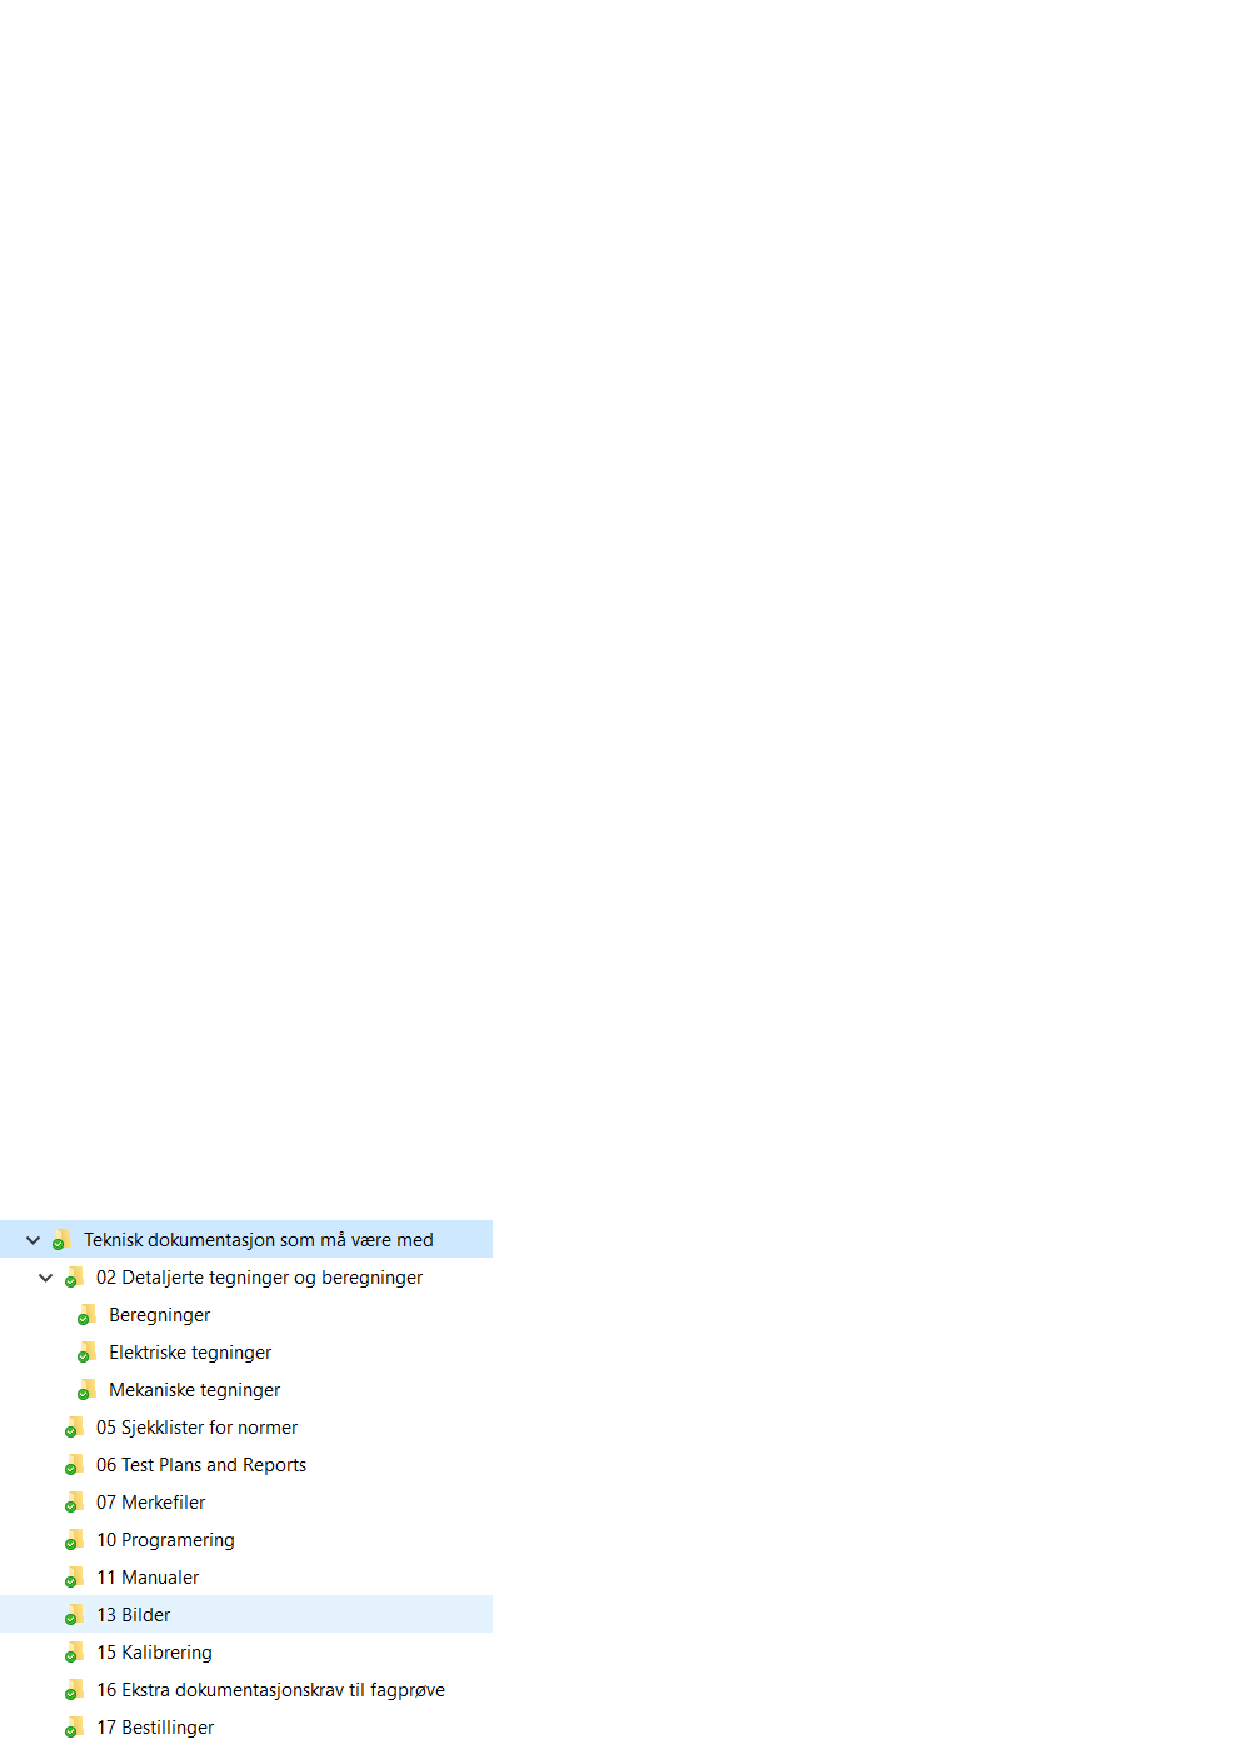
\includegraphics[bb = 0 0 200 100, draft, type=eps]{Gondol teknisk dokumentasjon.png}

Beregninger som skal gjøres:
\begin{itemize}
\item tilførselskabel
\item ledninger fra sikring til power (24V)
\end{itemize}
Tegninger som skal være med:
\begin{itemize}
\item komplette eltegninger
\item arrangementstegning
\item rekkeklemmeliste
\item IO-liste (også den fra PC|Schematic kalt PLS-liste)
\item Skykkliste
\item komponentliste
\end{itemize}
Sjekklister som skal være med:
\begin{itemize}
\item Sluttkontroll for elektrisk ustyr på maskiner
\end{itemize}
Test plan:
\begin{itemize}
\item Plan med avkryssningsruter for verifikasjon (sluttkontroll)
\end{itemize}
Merkefiler:
\begin{itemize}
\item alle filer som brukes til å skrive ut merking
\end{itemize}
Programmering:
\begin{itemize}
\item IO-liste
\item PLS planlegging
\item PLS program
\end{itemize}
Manualer:
\begin{itemize}
\item Manualer for alt utstyr som dere klarer å oppdrive. 
\end{itemize}
Bilder:
\begin{itemize}
\item Ta bilder av anlegge og legg inn her. 
\end{itemize}
Ekstra dokumentasjonskrav til fagprøve. 

Denne mappen er tenkt brukt til dokumentasjon som vi bruker her på
skole og som fagprøvenemden krever. som ikke er en del av den tekniske
dokumentajonen for en maskin.

Det skal være:
\begin{itemize}
\item Logg 
\item Planlegging av arbeidsoppdrag (fremdriftsplan)
\end{itemize}
Bestillinger:
\begin{itemize}
\item Alle bestillinger som dere har gjørt. 
\end{itemize}

\subsection{Ekstra oppgaver}

\subsubsection{Maskinsikkerhet Sikkerhetsrelatertedeler av styresystemer. }

Start av motor. 

Nullspenningsutløsning, bevegelig vern, sikker stopp, sikker start. 

\subsubsection{Oppkobling av sorteringsanlegg. }

\subsubsection{Oppkobling mot rytmeboks. }

\subsubsection{SSR-Rele}

\subsubsection{Motor via H-bro.}

\subsubsection{IO-sjekk Modbus RTU mot tretanker, Stasjon1, }

\subsubsection{Kalibrering av DP-celler på stasjoner. }

\subsection{Gamle prøver}

\subsubsection{Prøve I}
\begin{enumerate}
\item (3p)Målecelle på kapasitansprinsippet. Set på namn på delane og trykk-pilene.\\
\vspace{1cm}
\\
\includegraphics[width=0.4\textwidth,bb = 0 0 200 100, draft, type=eps]{Trykkprøve02.png}\vspace{1cm}
\item (3p)En motor med følende merkeskilt er koblet til et vanlig TN nett
i Norge. \\
 \includegraphics[width=0.3\textwidth,bb = 0 0 200 100, draft, type=eps]{Nameplate01.png}\\

\begin{enumerate}
\item (3p)Beregn motorens sakking i \%.
\item (3p)Hvor mange polpar har motoren ?
\item (3p)Hva blir fasestømmen og fasespenningen? 
\item (3p)Hva blir virkningsgraden?
\item (3p)Kan denne motoren brukes til en Y/D starter på dette nettet?
\end{enumerate}
\item (3p)Hvilke målinger ville du gjort for å sjekke om viklingene er i
orden på en indusjonsmotor, hvilke resultater forventer du?
\item (3p)Bildet viser en nødstopp, hvilken betydning har sirkelen med en
pil i?\\
\includegraphics[width=0.2\textwidth,bb = 0 0 200 100, draft, type=eps]{estop.png}
\item (3p)Hva menes med at nødstopp skal være et komplimentært sikkerhetstiltak. 
\item (3p)Vis med tegning hvordan du ville koble sammen disse to enhetene.Vis
også hvilke parametre som er viktige å he like på begge enhetene.
\\
\includegraphics[width=1\textwidth,bb = 0 0 200 100, draft, type=eps]{RS485Kobling.png}\\
\vspace{2cm}
\vspace{2cm}
\item (3p)Forklar korleis vi skal montere måleomformaren til prosessrøyret
når vi har veske- eller damptrykk i røyret. Grunngje forklåringa,
gjerne med ei skisse.
\item (3p)Tegn og forklar virkemåten til en asynkronmotor, ha spesiell fokus
på det roterende feltet. 
\item (3p)Tegn og forklar hva vi oppnår ved å koble sekundærsiden av en
styrestrømforsyning til PE.

\vspace{2cm}
Nå skal du levere inn papirdelen av prøven og finne frem PC.\vspace{2cm}

\item (3p)Du skal tegne vedlagt kretsskjema i PC|Schematic
\item (3p)Vedlagt finner du en modbus data tabell (data register). Her skal
du plukke ut registrene som er nødvendige for å starte og stoppe motoren,
som er koblet til frekvensomformeren. Start og stopp tider til frekvensomformeren
er ikke den del av oppgaven. Parameter H5-12=TRUE (1). Parametrere
til Frekvensomformeren er 19200 8N1. \\
Registrene du finner skal du legge inn i et Codesys prosjekt som du
skal bruke i neste oppgave. \newpage{}
\item (6p)Kornsilo

IO-Liste

\begin{tabular}{|c|c|c|}
\hline 
Tilkoblet utstyr & Variabel & Beskrivelse av tilkoblet utstyr\tabularnewline
\hline 
\hline 
Start Knapp & Start & \tabularnewline
\hline 
Stopp Knapp & Stopp & \tabularnewline
\hline 
H Sensor & LevelHigh & \tabularnewline
\hline 
L Sensor & LevelLow & \tabularnewline
\hline 
Drifts Lys & Drift & \tabularnewline
\hline 
Pumpe Lys & Pumpe & \tabularnewline
\hline 
Alarm Lys & AlarmLys & \tabularnewline
\hline 
Alarm Lyd & AlarmLyd & \tabularnewline
\hline 
\end{tabular}

En kornsilo skal fyllest ved hjelp av en pumpe

\includegraphics[width=0.5\textwidth,bb = 0 0 200 100, draft, type=eps]{Kornsilo.png}

Der er to nivåvakter i siloen (L og H) disse gir \textquotedblright{}
TRUE\textquotedblright{} når nivået ligger over giveren.

Virkemåte: Pumpa i en silo skal alltid starte når nivået er under
minimum og stoppe når nivået går over maksimum for siloen.\\
Det skal lages en enkel visualisering (tenk skapdør for styring av
anlegget) som gjør det mulig å teste programmet.
\begin{itemize}
\item Anlegget settes i drift med en Start knapp og stoppes med en Stoppknapp.
Når anlegget er satt i drift og nivået er under L startes pumpe P.
Denne går til nivået når H. Slik fortsetter det til driften av anlegget
stoppes.
\item Legg til en teller for totalt antall sykluser på pumpe.
\item Det skal aktiveres en alarm om det tar mer en 10min (10s) å komme
over L nivå (etter at den har vært under). Alarmen skal ha bekreft
og resett funksjon.
\end{itemize}

\item Det er har oppstått et behov for en ny nødstopp. All risikovurdering
er tatt og nytt koblingsskjema er tegnet (samme som du tegnet i tegneoppgaven).
Se også på oversiktstegningen om hvor nødstoppen -S10 plassereres. 
\begin{enumerate}
\item (3p)Planlegg gjennomføring av monteringen. 

Viktige deler av vurderingen vil være, fremdriftsplan, verktøyliste,
deleliste, bruk av dokumentasjon i vurderinger. 
\item (3p)Beskriv hvordan du ville gjennomført jobben

Viktige deler av vurderingen vil være detaljene i beskrivelsene og
en beskrivelsen er kronologisk. 
\item (3p)Dokumenter arbeidet. 

Viktige deler av vurderingen vil være om du har oversikt på hva som
skal oppdateres av dokumentasjon og kan synliggjøre dette. 
\end{enumerate}
\end{enumerate}
\includepdf{YaskawaModbusTable}

\includepdf[pages=-,angle=90]{\string"Prøve01 Tegninger\string"}

\subsubsection{Prøve II}
\begin{enumerate}
\item (6p)Vis med tegning hvordan du ville koble sammen disse to enhetene.Vis
også hvilke parametre som er viktige å ha like på begge enhetene.
\\
\includegraphics[width=1\textwidth,bb = 0 0 200 100, draft, type=eps]{RS485Kobling.png}\\
\vspace{2cm}
\vspace{2cm}
\newpage{}
\item (6p)
\begin{enumerate}
\item Nummerer kontaktsettene med både ordens- og funksjonssiffer
\item I hvilken rekkefølge vil singallpmpene -H1 til -H4 lyse når bryter
-S1 betjenes?\\
\includegraphics[width=1\textwidth,bb = 0 0 200 100, draft, type=eps]{releer01.png}\\
\end{enumerate}
\item (6p) Forklar følgende uttrykk i reguleringsteknikken:
\begin{itemize}
\item Prosessvariabel
\item Prosessverdi
\item Settpunkt
\item Pådrag
\item Pådragsorgan
\end{itemize}
\item (6p)
\begin{enumerate}
\item Beskriv hva en oppnår med å koble sekundærsiden av en styrestrømforsyning
til PE.
\item Hva menes med at nødstopp skal være et komplimentært sikkerhetstiltak. 
\end{enumerate}
\item (6p) Forklar virkemåter til en PID regulator, ta med funksjonen til
P, I og D leddet.\newpage{}
\item (6p)Bildene viser to måter å regulere nivået i en tank på. Forklar
hvilken av tankene som må da direktevirkende regulator og hvilkensom
må ha reverserende regulator.\\
a) \includegraphics[width=6cm,bb = 0 0 200 100, draft, type=eps]{Reverserende regulator.png}\hspace{2cm}b)
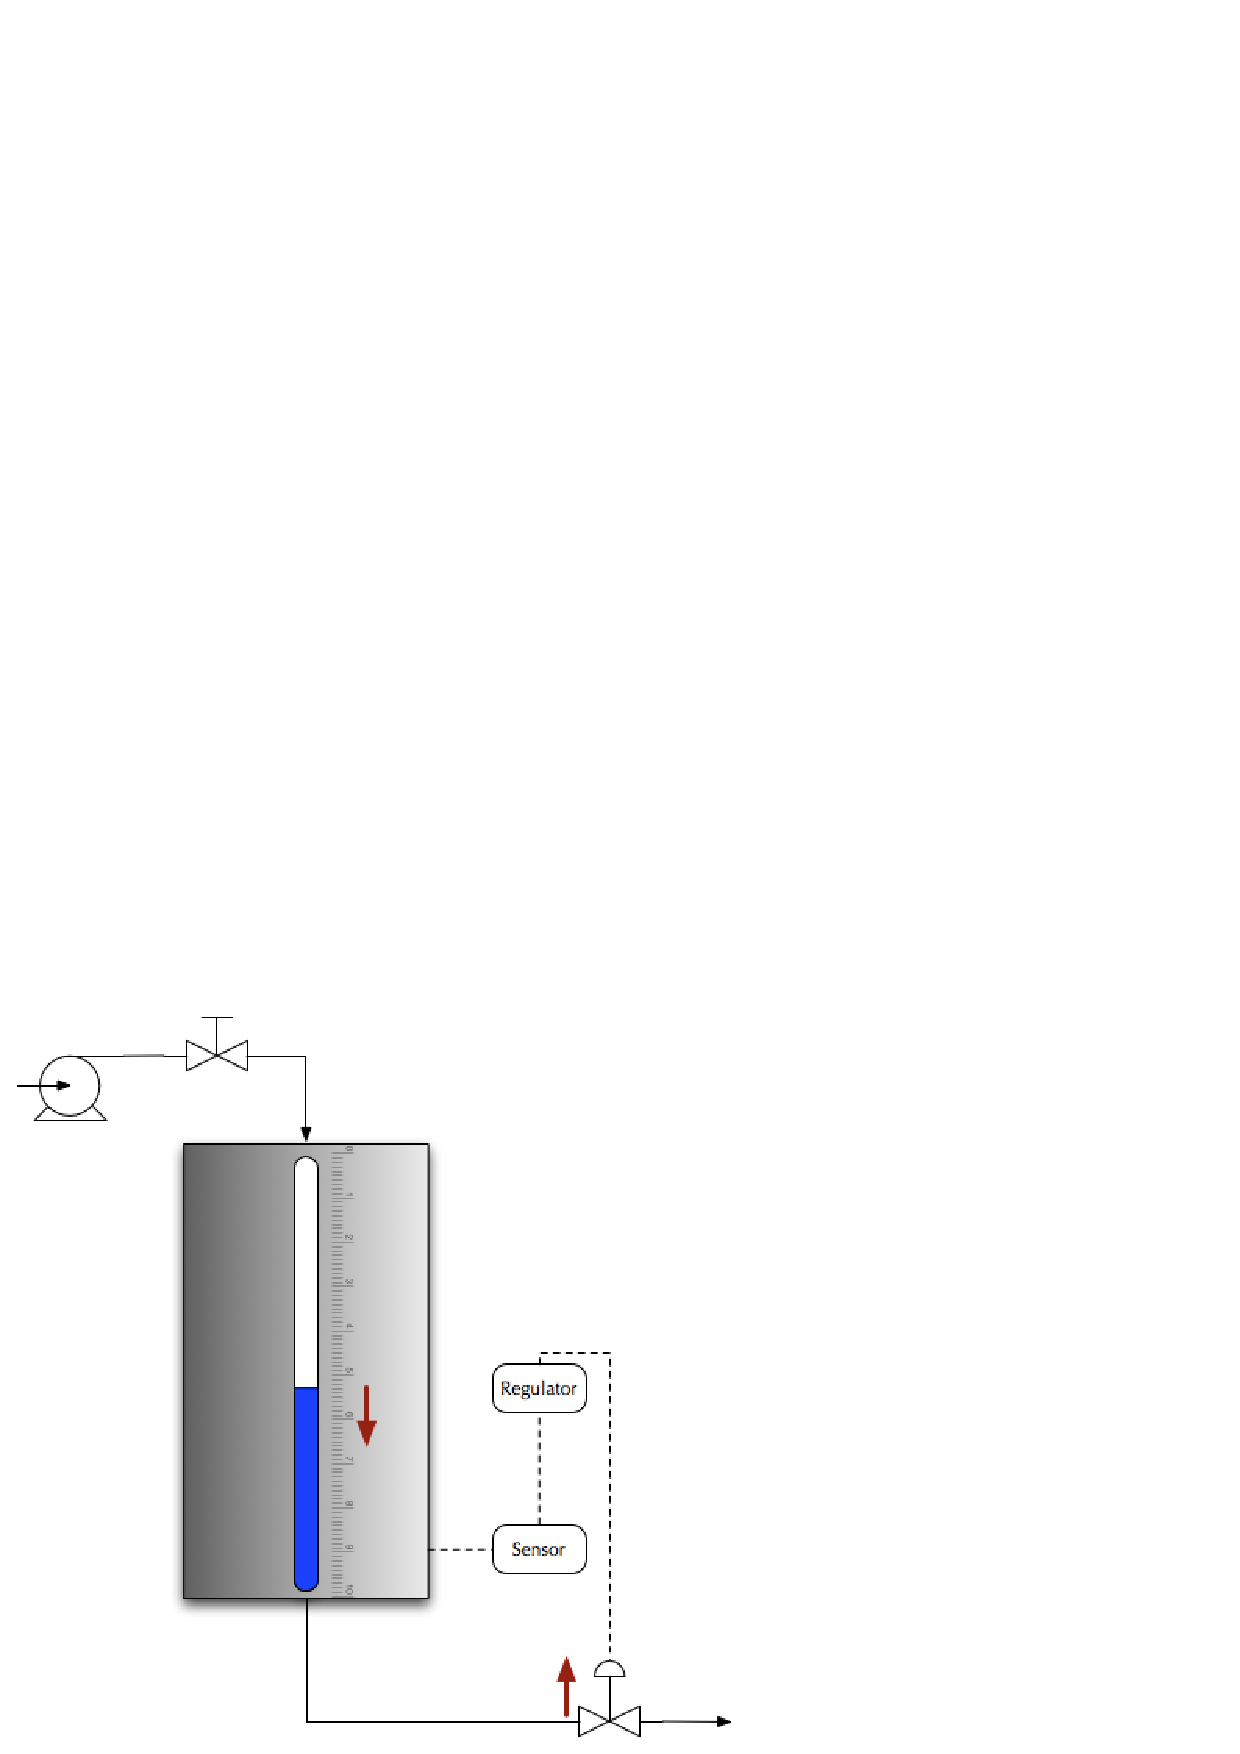
\includegraphics[width=6cm,bb = 0 0 200 100, draft, type=eps]{Direktevirkende regulator.png}

\vspace{2cm}
Nå skal du levere inn papirdelen av prøven og finne frem PC.\vspace{2cm}

\item (6p)Du skal tegne vedlagt kretsskjema i PC|Schematic\newpage{}
\item (6p)Kornsilo

IO-Liste

\begin{tabular}{|c|c|c|}
\hline 
Tilkoblet utstyr & Variabel & Beskrivelse av tilkoblet utstyr\tabularnewline
\hline 
\hline 
Start Knapp & Start & \tabularnewline
\hline 
Stopp Knapp & Stopp & \tabularnewline
\hline 
H Sensor & LevelHigh & \tabularnewline
\hline 
L Sensor & LevelLow & \tabularnewline
\hline 
Drifts Lys & Drift & \tabularnewline
\hline 
Pumpe Lys & Pumpe & \tabularnewline
\hline 
Alarm Lys & AlarmLys & \tabularnewline
\hline 
Alarm Lyd & AlarmLyd & \tabularnewline
\hline 
\end{tabular}

En kornsilo skal fyllest ved hjelp av en pumpe

\includegraphics[width=0.5\textwidth,bb = 0 0 200 100, draft, type=eps]{Kornsilo.png}

Der er to nivåvakter i siloen (L og H) disse gir \textquotedblright{}
TRUE\textquotedblright{} når nivået ligger over giveren.

Virkemåte: Pumpa i en silo skal alltid starte når nivået er under
minimum og stoppe når nivået går over maksimum for siloen.\\
Det skal lages en enkel visualisering (tenk skapdør for styring av
anlegget) som gjør det mulig å teste programmet.
\begin{itemize}
\item Anlegget settes i drift med en Start knapp og stoppes med en Stoppknapp.
Når anlegget er satt i drift og nivået er under L startes pumpe P.
Denne går til nivået når H. Slik fortsetter det til driften av anlegget
stoppes.
\item Legg til en teller for totalt antall sykluser på pumpe.
\item Det skal aktiveres en alarm om det tar mer en 10min (10s) å komme
over L nivå (etter at den har vært under). Alarmen skal ha bekreft
og resett funksjon.
\end{itemize}
\newpage{}
\item (12p)Det er har oppstått et behov for en ny nødstopp. All risikovurdering
er tatt og nytt koblingsskjema er tegnet (samme som du tegnet i tegneoppgaven).
Se også på oversiktstegningen om hvor nødstoppen -S10 plassereres. 
\begin{enumerate}
\item Planlegg gjennomføring av monteringen. 

Viktige deler av vurderingen vil være, fremdriftsplan, verktøyliste,
deleliste, bruk av dokumentasjon i vurderinger. 
\item Beskriv hvordan du ville gjennomført jobben

Viktige deler av vurderingen vil være detaljene i beskrivelsene og
en beskrivelsen er kronologisk. 
\item Dokumenter arbeidet. 

Viktige deler av vurderingen vil være om du har oversikt på hva som
skal oppdateres av dokumentasjon og kan synliggjøre dette. 
\end{enumerate}
\end{enumerate}
\includepdf[pages=-,angle=90]{\string"Prøve01 Tegninger\string"}

\subsubsection{Prøve III}
\begin{enumerate}
\item (6p)Vis med tegning hvordan du ville koble sammen disse to enhetene.Vis
også hvilke parametre som er viktige å ha like på begge enhetene.
\\
\includegraphics[width=1\textwidth,bb = 0 0 200 100, draft, type=eps]{RS485Kobling.png}\\
\vspace{2cm}
\vspace{2cm}
\newpage{}
\item (6p)S
\begin{enumerate}
\item Konsturer en krets som får signallampen -H1 til å blinke ved hjelp
av tidsreleene -K1 og -K2.\\
\includegraphics[width=1\textwidth,bb = 0 0 200 100, draft, type=eps]{releer02.png}\\
\end{enumerate}
\item (6p) Forklar følgende uttrykk i reguleringsteknikken:
\begin{itemize}
\item Forstillingsenhet
\item Autoj og manuell modus
\item Manipulerende variabel
\item Pådrag
\item Pådragsorgan
\end{itemize}
\item (6p)
\begin{enumerate}
\item Beskriv hva en oppnår med å koble sekundærsiden av en styrestrømforsyning
til PE.
\item Hva menes med at nødstopp skal være et komplimentært sikkerhetstiltak. 
\end{enumerate}
\item (6p) Forklar virkemåter til en PID regulator, ta med funksjonen til
P, I og D leddet.\newpage{}
\item (6p)Bildene viser to måter å regulere nivået i en tank på. Forklar
hvilken av tankene som må da direktevirkende regulator og hvilkensom
må ha reverserende regulator.\\
a) \includegraphics[width=6cm,bb = 0 0 200 100, draft, type=eps]{Reverserende regulator.png}\hspace{2cm}b)
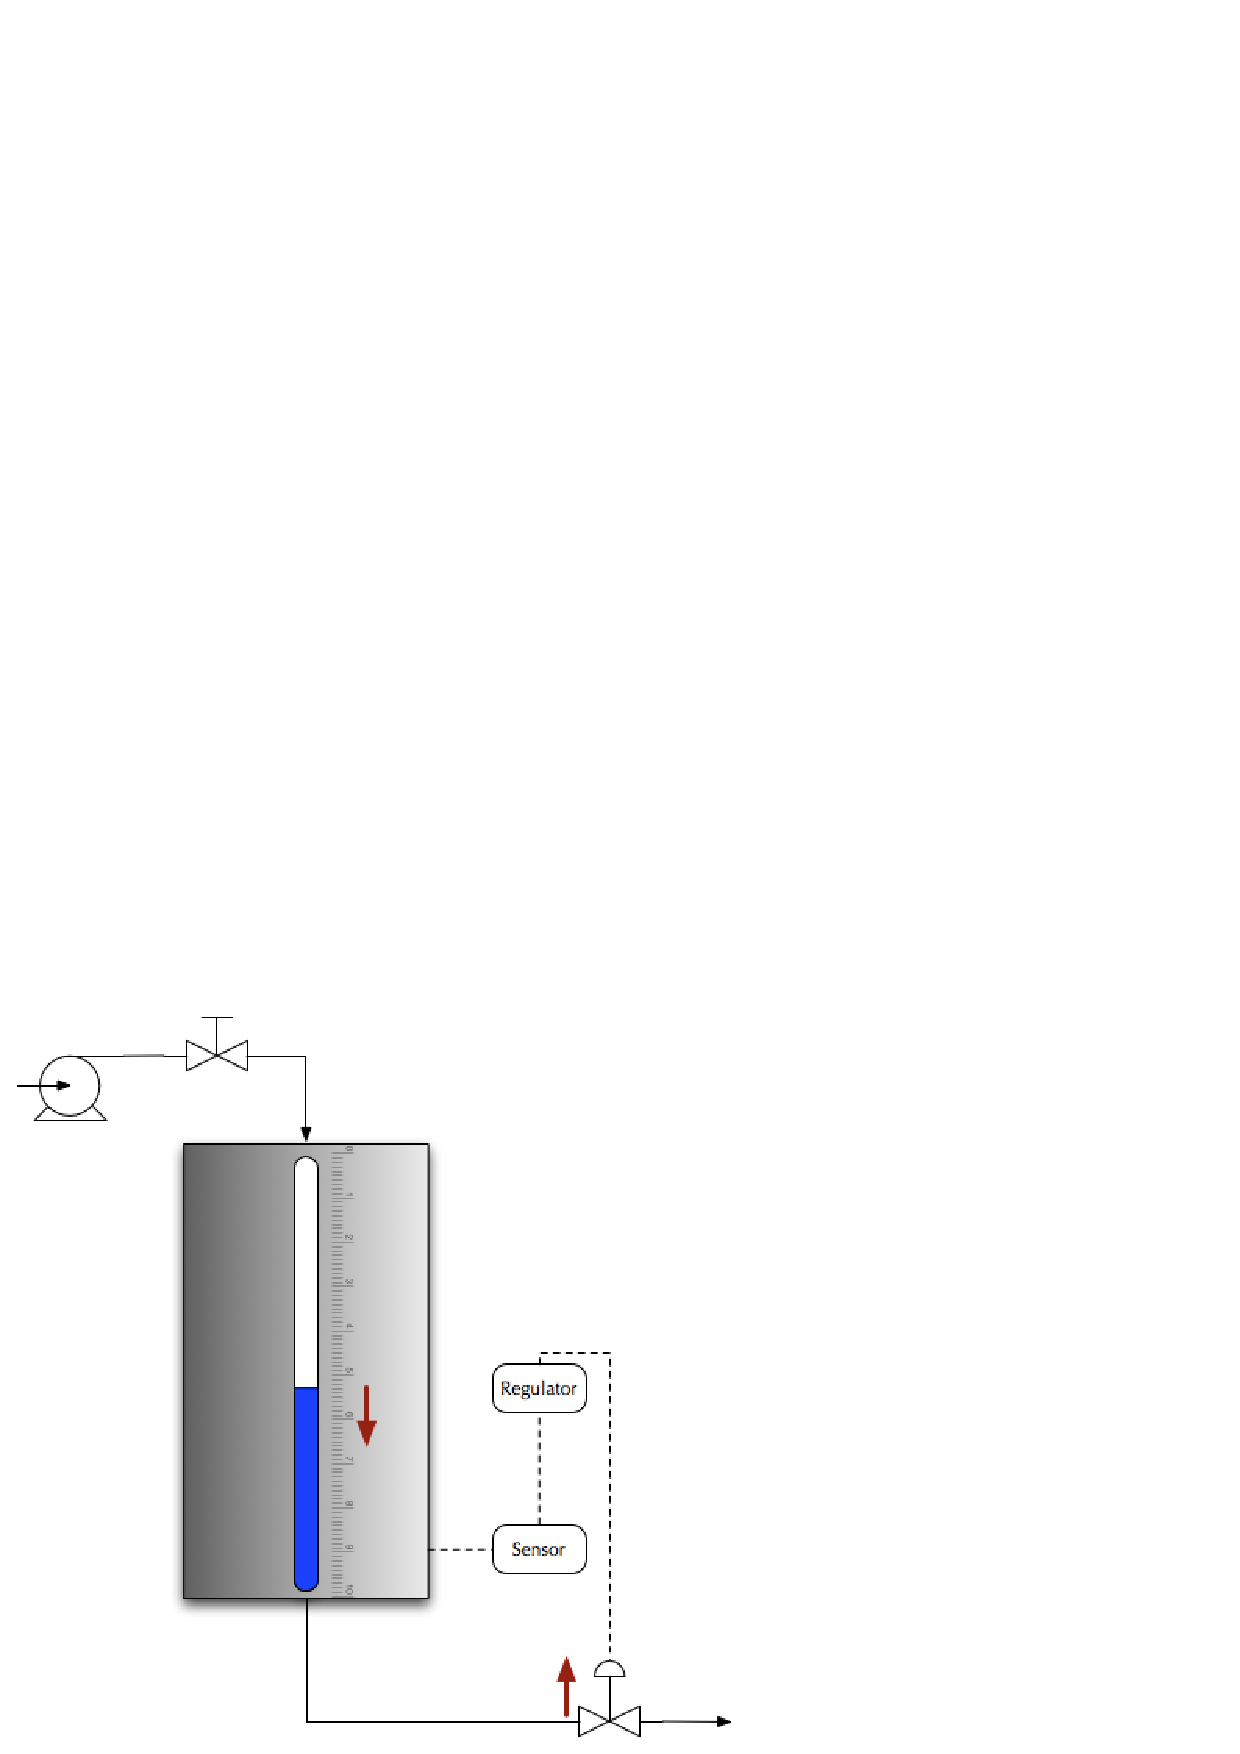
\includegraphics[width=6cm,bb = 0 0 200 100, draft, type=eps]{Direktevirkende regulator.png}

\vspace{2cm}
Nå skal du levere inn papirdelen av prøven og finne frem PC.\vspace{2cm}

\item (6p)Reguler inn prosessen i utdelt PLS program (Innstillingsoppgave
Gand reguleringsstasjon 02.project på utdelt USB-pinne) ved hjelp
av Skogestad. \\
Ta bilder og vis fremgangsmåte i et worddokumet. \\
Her må du laste inn programmet og kjøre dette på egen PC.\\
 (Det er forventet at eleven behersker alle deler av denne oppgaven
selv.)\newpage{}
\item (6p)Kornsilo

IO-Liste

\begin{tabular}{|c|c|c|}
\hline 
Tilkoblet utstyr & Variabel & Beskrivelse av tilkoblet utstyr\tabularnewline
\hline 
\hline 
Start Knapp & Start & \tabularnewline
\hline 
Stopp Knapp & Stopp & \tabularnewline
\hline 
H Sensor & LevelHigh & \tabularnewline
\hline 
L Sensor & LevelLow & \tabularnewline
\hline 
Drifts Lys & Drift & \tabularnewline
\hline 
Pumpe Lys & Pumpe & \tabularnewline
\hline 
Alarm Lys & AlarmLys & \tabularnewline
\hline 
Alarm Lyd & AlarmLyd & \tabularnewline
\hline 
\end{tabular}

En kornsilo skal fyllest ved hjelp av en pumpe

\includegraphics[width=0.5\textwidth,bb = 0 0 200 100, draft, type=eps]{Kornsilo.png}

Der er to nivåvakter i siloen (L og H) disse gir \textquotedblright{}
TRUE\textquotedblright{} når nivået ligger over giveren.

Virkemåte: Pumpa i en silo skal alltid starte når nivået er under
minimum og stoppe når nivået går over maksimum for siloen.\\
Det skal lages en enkel visualisering (tenk skapdør for styring av
anlegget) som gjør det mulig å teste programmet.
\begin{itemize}
\item Anlegget settes i drift med en Start knapp og stoppes med en Stoppknapp.
Når anlegget er satt i drift og nivået er under L startes pumpe P.
Denne går til nivået når H. Slik fortsetter det til driften av anlegget
stoppes.
\item Legg til en teller for totalt antall sykluser på pumpe.
\item Det skal aktiveres en alarm om det tar mer en 10min (10s) å komme
over L nivå (etter at den har vært under). Alarmen skal ha bekreft
og resett funksjon.
\end{itemize}
\newpage{}
\item (12p)Det er har oppstått et behov for en ny nødstopp. All risikovurdering
er tatt og nytt koblingsskjema er tegnet (samme som du tegnet i tegneoppgaven).
Se også på oversiktstegningen om hvor nødstoppen -S10 plassereres. 
\begin{enumerate}
\item Planlegg gjennomføring av monteringen. 

Viktige deler av vurderingen vil være, fremdriftsplan, verktøyliste,
deleliste, bruk av dokumentasjon i vurderinger. 
\item Beskriv hvordan du ville gjennomført jobben

Viktige deler av vurderingen vil være detaljene i beskrivelsene og
en beskrivelsen er kronologisk. 
\item Dokumenter arbeidet. 

Viktige deler av vurderingen vil være om du har oversikt på hva som
skal oppdateres av dokumentasjon og kan synliggjøre dette. 
\end{enumerate}
\end{enumerate}
\includepdf[pages=-,angle=90]{\string"Prøve01 Tegninger\string"}

\section{Gand Reguleringsstasjon\label{sec:Gand-Reguleringsstasjon}}

\begin{longtable}[c]{|>{\centering}p{0.75cm}|>{\raggedright}p{3cm}|>{\raggedright}p{4cm}|>{\raggedright}p{4cm}|c|>{\raggedright}p{2cm}|}
\hline 
Uke & Emne & Kompetansemål & Læremål  & Tid & Link\tabularnewline
\hline 
\endhead
\hline 
42 & Grunnleggende Reguleringsteknikk & Idriftsette og optimalisere regulatorer basert på prosessbehov & Beskrive en reguleringsløyfe (åpen og lukket)

Kunne bruke og beskrive faguttrykk for reguleringsteknik 

Kunne beskrive oppbyggningen til en PID-regulator og hvilken virkning
P, I og D parameteret har på utgangssignalet ved et spring på inngangsignale & 4 & \ref{sec:Grunnleggender-reguleringsteknik}\tabularnewline
\hline 
42 & PID Regulator på PLS og i HMI & Planlegge, programmere, montere og idriftsette programmerbare styresystemer & Kunne legge inn en funksjkonsblokk for PID regulering i Codesys og
konvertere analogverdier slik at de passer med denne.  & 3 & \ref{subsec:PIDiPLS}\tabularnewline
\hline 
45 & Optimalisering

Tim og Z\&N & Idriftsette og optimalisere regulatorer basert på prosessbehov & Kunne bruke tims roule of thumb, Z\&N svingemetode for å optimalisere
en prosess. &  & \tabularnewline
\hline 
45 & Optimalisering

Skogestad & Idriftsette og optimalisere regulatorer basert på prosessbehov & Kunne bruke skogestads metode for kjenne igjen selvstabiliserende
og integrerende prosesser og optimalisere disse prosessene & 2 & \tabularnewline
\hline 
43 & Beskrivelse av virkemåte & Tegne, lese og forklare instrumenterte prosessflytskjemaer og bruke
annen relevant dokumentasjon for automatiserte anlegg & Kunne tegne P \& ID av stasjonen og forklare virkemåtne. 

Kunne finne manualer til alt utstyr på stasjonen.  & 2 & \ref{sec:Gand-Reguleringsstasjon}\tabularnewline
\hline 
43 & Tegning av P\&ID & Tegne, lese og forklare instrumenterte prosessflytskjemaer og bruke
annen relevant dokumentasjon for automatiserte anlegg &  & 4 & \ref{sec:P-=000026-ID}\tabularnewline
\hline 
40 & Reguleringsstryktu-rer & Idriftsette og optimalisere regulatorer basert på prosessbehov & Kunne kjenne igjen kaskadekoblet regulering i et anlegg - Kunne forklare
prinsippet for reguleringsmetoden - Kunne sette opp en kaskadekoblet
regulering.

Kunne kjenne igjen foroverkoblet regulering i et anlegg - Kunne forklare
prinsippet for reguleringsmetoden - Kunne sette opp en foroverkoblet
regulering.

Kunne kjenne igjen forholdsregulering i et anlegg - Kunne forklare
prinsippet for reguleringsmetoden - Kunne sette opp regulatorer for
forholdsregulering & 4 & \tabularnewline
\hline 
 &  &  &  &  & \tabularnewline
\hline 
 &  &  &  &  & \tabularnewline
\hline 
45 & PDS	 &  &  & 8 & Teori

\ref{sec:PDS-Power-Drive}

Oppgaver

\ref{subsec:Oppgaver-til-PDS}\tabularnewline
\hline 
44 & Ethernet\\
TCP/IP

RS-485/Modbus & anvende ulike elektroniske kommunikasjonssystemer i automatiserte
anlegg &  & 3 & \tabularnewline
\hline 
43 &  &  &  & 8 & \tabularnewline
\hline 
 & Introduksjon til HPHMI & Endre og tilpasse skjermbilder for grensesnitt mellom menneske og
maskin & Vite hva HPHMI er

Vite at informasjon er data i en kontekst

Kunne kunne lage et navigeringssystem for HPHMI

Kunne ta i bruke en farge spesifikasjon i Codesys

Kunne ta i bruk symbol med struct data interface. & 2 & \ref{subsec:Introduksjon-til-High}\tabularnewline
\hline 
 & Reguleringsventil & montere og idriftsette ulike typer pådragsorganer med tilhørende forstillingselementer
og hjelpeutstyr\\
MekMål:

planlegge, gjennomføre og dokumentere vedlikehold av reguleringsventiler
og ventilutstyr etter leverandørens spesifikasjoner &  &  & \tabularnewline
\hline 
43 & Sekvens-programmering & planlegge, programmere, montere og idriftsette programmerbare styresystemer & Eleven skal kunne sette opp:

- Enkel sevkens

- alternative og parallelle sekvenser

- lage utgangsprogram med aut/man styring til et sekvensprogram.

- Styre regulator med sekvens & 12 & Teori:

\ref{subsec:Sekvensielle-styringer}

Oppgaver:

\ref{subsec:Oppgaver-til-sekvensstyring}\tabularnewline
\hline 
 &  &  &  &  & \tabularnewline
\hline 
 & Måling av Flow? & montere, konfigurere, kalibrere og idriftsettelse digitale og analoge
målesystemer &  &  & \tabularnewline
\hline 
 & Måling av Nivå & montere, konfigurere, kalibrere og idriftsettelse digitale og analoge
målesystemer &  &  & \tabularnewline
\hline 
43 & Sikkerhetsrele og sikkerhetsrelatertedelar av styresustemet & utføre risikovurdering og vurdere tiltak for ivaretakelse av person\textendash{}
og maskinsikkerhet & Kunne forklare hva som menes med sikkerhetsrelaterte deler av styresystemet. 

Kunne sette opp en enkel +24V-SAFE spenning til bruk av pådragsorganer. 

Kunnegjøre kobliner med enkle sikkerhetsreleer (Enkle er definert
som DE vi har i klasserommet).  & 4 & \ref{subsec:Sikkerhetsrele-og-sikkerhetsrela}

\href{http://www.omron.com.au/service_support/technical_guide/safety_component/safety_circuit_example.asp}{Omron side med koblinger}\tabularnewline
\hline 
 &  &  &  &  & 		\tabularnewline
\hline 
46 & Alarmer i codesys &  &  &  & \tabularnewline
\hline 
\end{longtable}

Gand reguleringsstasjon er en reguleringsmodell, tiltenkt bruk på
skoler, for undervisning i reguleringsteknikk. 

Prøvestasjonen inneholder to vanntanker koblet sammen med rør, reguleringsventil
og pumpe. Det pumpes vann inn i tanken, og sleppes ut vann med en
reguleringsventil. Det er instrumentering for måling av nivå og strømning. 

Instrumenteringen på stasjonen kan bestå av: 

\textbullet{} Ultralyd nivåføler

\textbullet{} Turbin Strømningsmåler

\textbullet{} Frekvensomformerstyrt pumpe

\textbullet{} Reguleringsventil.

\textbullet{} Wago PFC 200 PLS (med Codesys runtime)

Enkle funksjoner på stasjonen skal kunne styres fra styrepanel på
stasjonen. I vanlig bruk skal det være mulig for elever å koble seg
opp til stasjonen v.h.a. nettleser og styre den med HMI. 


\subsection{Gruppe oppgaver til Gand Reguleringsstajson}

\subsubsection{Kontroll av dokumentasjon}

Dere skal gå igjennom dokumentasjonen til stasjonen og sjekke at stasjonen
er i henhold til denne. Avvik skal noteres, og dokumentasjon skal
oppdateres. 

\subsubsection{IO-sjekk}

Dere skal gjøre en sjekk av alle IO på stasjonen. 

Det skal settes opp en sjekkliste for alle IO-er og det skal utarbeides
en plan for hvordan sjekken skal foregå. 

\subsection{Individuelle arbeidsoppdrag på Gand Reguleringsstajson}

\subsubsection{Kalibrering av en LT}

\subsubsection{Tegning av skjema for omkobling av stasjon (arrangementstegning, }

\subsubsection{Sette opp kommunikasjon mot stasjon på teknisk nett. }

\subsubsection{Oppsett av PDS (med kommunikajons)}

\subsubsection{Lage eget styreprogram for stasjonen. }

\section{Fabrikkautomasjon (Diskret Automasjon)}

Hva er diskret automasjon? Det er produksjon av deler som kan telles.

\begin{longtable}[c]{|>{\centering}p{0.75cm}|>{\centering}p{3cm}|>{\raggedright}p{4cm}|>{\raggedright}p{4cm}|c|>{\centering}p{2cm}|}
\hline 
Uke & Emne & Kompetansemål & Læremål & Tid & Link\tabularnewline
\hline 
\endhead
\hline 
4 & Anleggsforståelse & Tegne, lese og forklare instrumenterte prosessflytskjemaer og bruke
annen relevant dokumentasjon for automatiserte anlegg & Kunne lese og forstå anleggsdokumentasjon som oppgitt i forberedelses
del til eksamen & 4t & \tabularnewline
\hline 
5 & 60204-1 elektrisk utstyr i maskiner & bruke gjeldende regelverk og normer for installasjon av elektroniske
kommunikasjonssystemer & Bruke 60204-1 i design av styring til stasjonen.

- å kunne blokkskjema for maskin med tilhørende referansenummer.

-Spesielt prioriterte kapittel 8, 9, 13. & 6t & \tabularnewline
\hline 
6 & Maskinsikkerhet &  &  & 2t & Teori:

\ref{subsec:Sikkerhetsrele-og-sikkerhetsrela}\tabularnewline
\hline 
7 & PDS &  &  & 4t & Teori

\ref{sec:PDS-Power-Drive}

Oppgaver

\ref{subsec:Oppgaver-til-PDS}\tabularnewline
\hline 
\end{longtable}

\section{Machine Control Interface}

MCI provides the necessary hardware interface and software control
for the drill floor, BOP handling and other drilling equipment which
do not have a dedicated programmable logic controller (PLC) control
cabinet or machine controller. With the MCI, these machines can easily
be integrated within the Drilling Control Network. The MCI is modular,
meaning it can be easily expanded to include new equipment or changes
made in the existing hardware configuration for additional machine
functionality. It is safe, easy to maintain and has a high reliability
rate. 

f%
\begin{longtable}[c]{|>{\centering}p{0.75cm}|>{\centering}p{3cm}|>{\raggedright}p{4cm}|>{\raggedright}p{4cm}|c|>{\centering}p{2cm}|}
\hline 
Uke & Emne & Kompetansemål & Læremål  & Tid & Link\tabularnewline
\hline 
\endhead
\hline 
 & Gjennomgang av anlegg & 7. anvende ulike elektroniske kommunikasjonssystemer i automatiserte
anlegg & Kunne beskrive alle masinene som styres av MCI skapet

Kunne forklare hvordan kommunikasjonen er internt i skapet. 

Kunne koble opp mot en RIO og få tilgang på IO signaler fra denn.  & 2 & Se presentasjoner i fagbibliotek. \tabularnewline
\hline 
 & Gjennomgang av skjema & tegne, lese og forklare instrumenterte prosessflytskjemaer og bruke
annen relevant dokumentasjon for automatiserte anlegg & Kunne følge koblinger igjennom skjema.  & 2 & \tabularnewline
\hline 
 &  &  &  &  & \tabularnewline
\hline 
 &  &  &  &  & \tabularnewline
\hline 
 & Måling av masse & Montere, konfigurere, kalibrere og idriftsettelse digitale og analoge
målesystemer &  &  & \tabularnewline
\hline 
 & Nødstopp i soner?? & Bruke gjeldende regelverk og normer for elektriske installasjoner
på maskiner &  &  & \tabularnewline
\hline 
 & Proporsjonal ventil hastighetsstyring & Montere og idriftsette ulike typer pådragsorganer med tilhørende forstillingselementer
og hjelpeutstyr &  &  & \tabularnewline
\hline 
 & trådløs styring.  & Bruke gjeldende regelverk og normer for elektriske installasjoner
på maskiner &  &  & \tabularnewline
\hline 
 & Skjemalesing & Tegne, lese og forklare instrumenterte prosessflytskjemaer og bruke
annen relevant dokumentasjon for automatiserte anlegg &  &  & \tabularnewline
\hline 
\end{longtable}

\subsection{Intro}

\subsubsection{Mousehole Racking System }

\subsubsection{Pipe Handling Catwalk Machine Incl Tail in Arm }

\subsubsection{Utility Winch 4, 5, 6 \& 10T Utility Winch 1, Moonpool }

\subsubsection{High Pressure Air Systems }

\subsubsection{X-Mas Tree Bridge Crane }

\subsubsection{Guide Arm }

\subsubsection{Oppgaver til MCI introduksjon}
\begin{enumerate}
\item Hvilke typer maskiner styres av MCI 2 Skapet?
\item I fagbiblioteket finner du frem Fagbibliotek\textbackslash Biblioteker\textbackslash Div\textbackslash Device
Descriptions\textbackslash Siemens\textbackslash im153-4\textbackslash GSDML-V2.3-Siemens-ET200M-20140709.xml
\end{enumerate}

\subsection{Skjema}

\subsubsection{Oppgaver til skjema}
\begin{enumerate}
\item Mousehole Winch. Hvilken type kabel brukes til winch brake release
ON/OF?
\item På hvilken rekkeklemme finner de styringen til denne i hovedskapet?
\item Hvilken rekkeklemme får -D18/0 driftsspenning fra?
\item Hva er -D18/1:2 reservert for? 
\item Følg +24V fra -D26/1: 15 til spenningskilden. 
\end{enumerate}

\section{Byggautomatiseringsanlegg (Stasjon 6)}

\begin{longtable}[c]{|>{\centering}p{0.75cm}|>{\centering}p{3cm}|>{\raggedright}p{4cm}|>{\raggedright}p{4cm}|c|>{\centering}p{2cm}|}
\hline 
Uke & Emne & Kompetansemål & Læremål  & Tid & Link\tabularnewline
\hline 
\endhead
\hline 
 &  &  &  &  & \tabularnewline
\hline 
\end{longtable}

Dette kapittelet er laget ut fra presentasjon gitt av KE Automasjon

Byggautomatiseringanlegg eller SD-anlegg er to ting av samme sak.
Det er anlegg som styrer bygg. 

Arbeidsoppgavene til en automatikker innen byggautomatisering kan
være:
\begin{itemize}
\item Rådgivning av kunder 
\item Samhandling mellom tekniske fag \textendash{} lede prosessen
\item Prosjektere anleggene \textendash{} tegning \textendash{} beregning
\item Programere plsèr og IT-system
\item Igangkjøring \textendash{} test \textendash{} sluttkontroll
\item Sluttdokumentasjon
\item Opplæring av kunder
\item Driftstøtte til kunder
\item Oppfølging av kunder og anlegg - service
\end{itemize}

\subsection{Bestandeler i et byggautomatiseringanlegg}
\begin{itemize}
\item Feltkomponenter/pådragsorgan
\begin{itemize}
\item Følere, ventiler, frekvensomformere, målere\dots{}
\end{itemize}
\item Undersentraler
\begin{itemize}
\item Programerbare enheter for styring av feltkomponenter
\end{itemize}
\item Toppsystem/scada
\begin{itemize}
\item PC/server med programvare for visning og logging av data hentet fra
undersentralene
\end{itemize}
\end{itemize}
\includegraphics[width=1\textwidth,bb = 0 0 200 100, draft, type=eps]{Byggautomasjon01.png}

\subsubsection{Feltkomponenter}

Feltkomponenter finnes i uttalige utførelserer, måleprinsipp og med
forskjellige feltbusløsning. Valget her styres av funksjonalitet,
kabling, datamengde osv. 

Felt tilkoblinger er måten informasjonen fra komponenten fraktes til
undersentralen.

\begin{figure}[H]
\begin{centering}
\includegraphics[bb = 0 0 200 100, draft, type=eps]{Byggautomasjon02.png}
\par\end{centering}
\caption{Eks: En romføler som registrerer temperatur/CO2/fukt, kommuniserer
med undersentral på Modbus}
\end{figure}

\begin{figure}[H]
\begin{centering}
\includegraphics[bb = 0 0 200 100, draft, type=eps]{Byggautomasjon03.jpg}
\par\end{centering}
\caption{Eks: {*} Romføler som registrerer temperatur {*} Motstandsmåling {*}
Kabelmotstand}
\end{figure}

\begin{figure}[H]
\begin{centering}
\includegraphics[bb = 0 0 200 100, draft, type=eps]{Byggautomasjon04.jpg}
\par\end{centering}
\caption{Eks: {*} Ventil som åpner for varmt vann {*} 0-10V {*} Mp bus og Modbus}
\end{figure}


\subsubsection{Undersentraler}

Undersentraler finnes i mange ulike typer fra ulike produsenter, og
med ulike ambisjonsnivåer. De kan være konfigurerbare, programmerbare
og fritt programmerbare. Undersentraler er plsèr, microkontrollere
ol. 

Automasjonsbus/bacbone er måten informasjonen fraktes fra undersentral
til undersentral eller undersentral til toppsystem 

\begin{figure}[H]
\begin{centering}
\includegraphics[bb = 0 0 200 100, draft, type=eps]{Byggautomasjon05.png}
\par\end{centering}
\caption{PLS som er fritt programerbar. Kan moduloppbygges og kan tilpasses.
Fås med mange ulike kommunikasjonsgrensesnitt }
\end{figure}

\begin{figure}[H]
\begin{centering}
\includegraphics[bb = 0 0 200 100, draft, type=eps]{Byggautomasjon06.jpg}
\par\end{centering}
\caption{Microkontroller er programerbar/konfigurerbar. Fast I/O. Kommunikasjonsgrensesnitt
er fast }
\end{figure}


\subsubsection{Feltkomponenter med logikk}

Det finnes systemer med feltkomponenter som har innebygget logikk
som man konfigurerer opp mot andre komponenter. Eksempel på dette
er KNX og DALI systemer. Dette er systemer som ikke egner seg i større
bygg. Hver komponent må konfigueres for seg, noe som skaper en lite
effektiv måte å jobbe på når byggene blir større. 

\begin{figure}[H]
\begin{centering}
\includegraphics[bb = 0 0 200 100, draft, type=eps]{Byggautomasjon07.jpg}
\par\end{centering}
\caption{Eksempel på anlegg med KNX logikk komponenter }
\end{figure}


\subsubsection{Toppsystem \textendash{} Scada system - HMI}

Toppsystemet, scada systemet er PC/server delen av et SD-anlegg og
har flere funksjoner:

Fungerer som brukergrensesnittet mellom bruker og automatikk. Historiske
data logges og vises. Alarmer vises, logges og sendes ut til bruker
Her finnes det også utallige systemer og varianter, både lokale og
sentrale. Eksempler kan være Iconics, IGSS eller WINCC

\begin{figure}[H]
\begin{centering}
\includegraphics[width=1\textwidth,bb = 0 0 200 100, draft, type=eps]{Byggautomasjon08.png}
\par\end{centering}
\caption{Eksempel fra toppsystem}
\end{figure}


\subsection{Kommunikasjonsmodellen}

\begin{figure}[H]
\begin{centering}
\includegraphics[width=1\textwidth,bb = 0 0 200 100, draft, type=eps]{Byggautomasjon09.jpg}
\par\end{centering}
\caption{Eksempel fra toppsystem}
\end{figure}

\begin{figure}[H]
\begin{centering}
\includegraphics[width=1\textwidth,bb = 0 0 200 100, draft, type=eps]{Byggautomasjon10.png}
\par\end{centering}
\caption{Eksempel fra toppsystem}
\end{figure}

I 3AUA skal vi kunne: 
\begin{itemize}
\item Modbus RTU
\item Modbus TCP
\item OPC UA
\item (MQTT)
\item EtherCat
\end{itemize}
Andre viktige busser i byggautomasjon er:
\begin{itemize}
\item M-Bus\\
M-Bus (Meter-Bus) er en Europeisk standard for fjernavlesning av varmemengdemålere,
KW timetellere eller andra typer forbruksmålere.
\end{itemize}

\subsubsection{Rom løsning}

\begin{figure}[H]
\begin{centering}
\includegraphics[width=1\textwidth,bb = 0 0 200 100, draft, type=eps]{Byggautomasjon11.png}
\par\end{centering}
\caption{Romløsning}
\end{figure}


\subsubsection{Teknisk Rom}

\begin{figure}[H]
\begin{centering}
\includegraphics[width=1\textwidth,bb = 0 0 200 100, draft, type=eps]{Byggautomasjon12.png}
\par\end{centering}
\caption{Teknisk Rom}
\end{figure}


\subsubsection{Kommunikasjon i hele anlegget}

\begin{figure}[H]
\begin{centering}
\includegraphics[width=1\textwidth,bb = 0 0 200 100, draft, type=eps]{Byggautomasjon13.png}
\par\end{centering}
\caption{Mot toppsystem}
\end{figure}

\begin{figure}[H]
\begin{centering}
\includegraphics[width=1\textwidth,bb = 0 0 200 100, draft, type=eps]{Byggautomasjon14.png}
\par\end{centering}
\caption{Ett bygg}
\end{figure}


\subsection{Standalone, integrere eller visualisere?}
\begin{itemize}
\item Hvordan skal systemet virke?
\item Hva skal kunne betjenes og hvorfor?
\item Har systemet informasjon som skal brukes i andre system?
\item Har systemet behov for informasjon fra andre system? 
\end{itemize}
\begin{figure}[H]
\begin{centering}
\includegraphics[width=1\textwidth,bb = 0 0 200 100, draft, type=eps]{Byggautomasjon15.png}
\par\end{centering}
\caption{Standalone enheter, virker bra hver for seg. }
\end{figure}

\begin{figure}[H]
\begin{centering}
\includegraphics[width=1\textwidth,bb = 0 0 200 100, draft, type=eps]{Byggautomasjon16.png}
\par\end{centering}
\caption{Visualisering}
\end{figure}

\begin{figure}[H]
\begin{centering}
\includegraphics[width=1\textwidth,bb = 0 0 200 100, draft, type=eps]{Byggautomasjon17.png}
\par\end{centering}
\caption{Visualisering}
\end{figure}

\begin{figure}[H]
\begin{centering}
\includegraphics[width=1\textwidth,bb = 0 0 200 100, draft, type=eps]{Byggautomasjon18.jpg}
\par\end{centering}
\caption{Optimal drift forutsetter god samkjøring mellom tekniske systemer}
\end{figure}


\subsection{Byggautomasjon og inneklima}

Ventilasjon, luftskifte og temperatur - en forutsetning for godt inneklima
(naaf.no)

\subsubsection{Inneklima}

Termisk miljø \textendash{} som har med temperaturkvalitet å gjøre

Atmosfærisk miljø \textendash{} som har med luftkvalitet å gjøre

Akustisk miljø \textendash{} som har med lydkvalitet å gjøre

Aktinisk miljø \textendash{} som har med lys- og strålingskvalitet
å gjøre

Mekanisk miljø \textendash{} som har med vibrasjoner å gjøre

\begin{figure}[H]
\begin{centering}
\includegraphics[width=0.5\textwidth,bb = 0 0 200 100, draft, type=eps]{Byggautomasjon19.jpg}
\par\end{centering}
\caption{Variabler for et godt inneklima}
\end{figure}


\subsubsection{HENØK}

Energiøkonomisering (ENØK) er i høyeste grad nødvendig, men må ikke
gjennomføres slik at innemiljøet blir helseskadelig. 

Helse må settes først! Dårlig helse fører til dårligere økonomi både
for den enkelte og for samfunnet og med betydelig større tap enn gevinstene
ved feilaktig ENØK. 

Derfor er det Helse- og energiøkonomisering = HENØK - som gir de beste
økonomiske løsningene!

Energiøkonomisering og helse (ENØK og HENØK) HENØK for bedre helse
og bedre økonomi! 

\begin{figure}[H]
\begin{centering}
\includegraphics[width=0.3\textwidth,bb = 0 0 200 100, draft, type=eps]{Byggautomasjon20.PNG}
\par\end{centering}
\caption{HENØK ?}
\end{figure}


\subsubsection{Romregulering}

Regulering av varme - temperatur

Regulering av kjøling - temperatur

Regulering av luft \textendash{} temperatur \textendash{} luftkvalitet
\textendash{} fukt - tilstedeværelse

Lys \textendash{} tilstedeværelse - lysmengde 

\paragraph{Temperatur}
\begin{itemize}
\item Temperaturforhold er viktige for menneskers helse, trivsel og funksjon
\item Dette er også viktig for evt vekst av mikroorganismer og husstøvmidd
m.m. som kan bidra til allergi, astma og inneklimasyke 
\item Temperaturen er viktig for graden av emisjon av kjemiske stoffer (gasser)
fra forskjellige kilder, og kan bidra til inneklimasyke 
\item Alt tatt i betraktning anbefales en operativ innetemperatur på ca.
19-22° C, men noe lavere ved høy fysisk aktivitet 
\item Både for høy og for lav innetemperatur kan bidra til dårligere helse,
dårlig trivsel og nedsatt arbeidsevne. 
\item Ved individuelle opplevelser av en bestemt innetemperatur bør hver
person tilpasse seg med bruk av hensiktsmessig bekledning 
\end{itemize}

\paragraph{Hvilken temperatur?}

\begin{figure}[H]
\begin{centering}
\includegraphics[width=0.5\textwidth,bb = 0 0 200 100, draft, type=eps]{Byggautomasjon21.PNG}
\par\end{centering}
\caption{Figuren viser at både muskulær og intellektuell arbeidsevne synker
ved for lav og for høy temperatur, mens ulykkesfrekvensen øker.}
\end{figure}

Alt tatt i betraktning anbefales en operativ innetemperatur på ca.
19-22° C 

Når flere mennesker oppholder seg i et rom, vil det vanligvis være
noen (opp til 20\%) som er misfornøyd med temperaturen uansett hva
den er. 

\paragraph{Vanlige problemstillinger}
\begin{itemize}
\item Feilinnstilt varmekilde eller termostat 
\item Manglende hensyn til brukernes helse, trivsel og funksjon ved energisparing
(feilslått ENØK). 
\item Feilplassert varmekilde (evt takvarme) 
\item For trege oppvarmingssystemer 
\item Sterk solinnstråling eller annen varmestråling 
\item Kaldras
\item Trekk fra vinduer, ventilasjonsanlegg 
\item Uhensiktsmessig bekledning 
\end{itemize}
\begin{figure}[H]
\begin{centering}
\includegraphics[width=1\textwidth,bb = 0 0 200 100, draft, type=eps]{Byggautomasjon22.PNG}
\par\end{centering}
\caption{Temperatur i ulike rom.}
\end{figure}

\begin{figure}[H]
\begin{centering}
\includegraphics[width=1\textwidth,bb = 0 0 200 100, draft, type=eps]{Byggautomasjon23.PNG}
\par\end{centering}
\caption{CO2 i ulike rom.}
\end{figure}

\begin{figure}[H]
\begin{centering}
\includegraphics[width=1\textwidth,bb = 0 0 200 100, draft, type=eps]{Byggautomasjon24.PNG}
\par\end{centering}
\caption{Innstilling i rom}
\end{figure}


\subsection{Ventilasjon og inneklima}

Regulering av varme - temperatur

Regulering av kjøling - temperatur

Regulering av luftmengde \textendash{} mengde - turtall

Regulering av trykk \textendash{} trykk - turtall

God ventilasjon skal sørge for: 
\begin{itemize}
\item Tilførsel av tilstrekkelige mengder ren luft
\item Fjerne lukt og forurensninger (støv, avgassinger)
\item Fjerne fuktighet i inneluften
\item Bygninger ska ha ventilasjon tilpasset rommenes forurensnings- og
fuktbelastning
\item CO2 er en god indikator på luftskifte 
\item CO2 skal ligge under <1000ppm 
\end{itemize}
Dårlig ventilasjon gir helseplager:
\begin{itemize}
\item Hodepine
\item Konsentrasjonsproblemer
\item Tung i hodet
\item Tretthet
\item Forverring av astma/allergi
\item økt forekomst av husstøvmidd
\item Hyppigere luftveisinfeksjoner
\item Lavere produktivitet
\end{itemize}

\subsubsection{Naturlig ventilasjon}

Ved naturlig ventilasjon er det oppdriftskrefter og vind som sørger
for at luften beveger seg gjennom bygningen. 

\begin{figure}[H]
\begin{centering}
\includegraphics[width=1\textwidth,bb = 0 0 200 100, draft, type=eps]{Byggautomasjon25.PNG}
\par\end{centering}
\caption{Naturlig ventilasjon}
\end{figure}


\subsubsection{Enkel mekanisk avtrekksventilasjon}

Ved enkel mekanisk avtrekksventilasjon brukes avtrekksvifte for å
bevege luften gjennom bygningen 

\begin{figure}[H]
\begin{centering}
\includegraphics[width=1\textwidth,bb = 0 0 200 100, draft, type=eps]{Byggautomasjon26.PNG}
\par\end{centering}
\caption{Enkel mekanisk avtrekksventilasjon}
\end{figure}


\subsubsection{Hybrid ventilasjon}

Ved hybrid ventilasjon utnyttes de naturlige kreftene som drivkraft
når disse er tilgjengelige til å bevege luften gjennom bygningen.
Under andre omstendigheter brukes vifter som drivkraft. 

\begin{figure}[H]
\begin{centering}
\includegraphics[width=1\textwidth,bb = 0 0 200 100, draft, type=eps]{Byggautomasjon27.PNG}
\par\end{centering}
\caption{Hybrid Ventilasjon}
\end{figure}


\subsubsection{Balansert ventilasjon}

Ved mekanisk balansert ventilasjon brukes mekaniske vifter til å bevege
luften gjennom bygningen. 

\begin{figure}[H]
\begin{centering}
\includegraphics[width=1\textwidth,bb = 0 0 200 100, draft, type=eps]{Byggautomasjon28.PNG}
\par\end{centering}
\caption{Balansert ventilasjon}
\end{figure}

\begin{figure}[H]
\begin{centering}
\includegraphics[width=1\textwidth,bb = 0 0 200 100, draft, type=eps]{Byggautomasjon29.PNG}
\par\end{centering}
\caption{Ventilasjonsagregat med balansering}
\end{figure}


\subsubsection{Ventilasjon av rom}

\begin{figure}[H]
\begin{centering}
\includegraphics[width=0.5\textwidth,bb = 0 0 200 100, draft, type=eps]{Byggautomasjon30.png}\includegraphics[width=0.5\textwidth,bb = 0 0 200 100, draft, type=eps]{Byggautomasjon31.png}
\par\end{centering}
\caption{Fortrengningsventilasjon}
\end{figure}

\begin{figure}[H]
\begin{centering}
\includegraphics[width=0.5\textwidth,bb = 0 0 200 100, draft, type=eps]{Byggautomasjon32.png}\includegraphics[width=0.5\textwidth,bb = 0 0 200 100, draft, type=eps]{Byggautomasjon33.png}
\par\end{centering}
\caption{Omrøringsventilasjon/spyling}
\end{figure}


\subsubsection{Vanlige problemstillinger}

Svært ofte skyldes problemer med ventilasjonsanleggene manglende eller
feil ved drift og vedlikehold 
\begin{itemize}
\item Drift og vedlikehold: 
\item Skifte filter
\item Sjekke at anlegget leverer den luftmengden den skal
\item Hold luftinntaket tørt og rent!!
\item Luftinntak lett tilgjengelig forinspeksjon, rengjøring, filterskifte 
\item Rett temperatur på tilluft
\end{itemize}
\begin{figure}[H]
\begin{centering}
\includegraphics[width=1\textwidth,bb = 0 0 200 100, draft, type=eps]{Byggautomasjon34.jpg}
\par\end{centering}
\caption{Tett filter}
\end{figure}


\subsubsection{Vanlige problemstillinger utover drift og vedlikehold}
\begin{itemize}
\item Ventilasjonsanlegg som er underdimensjonert
\item Luftskiftet i oppholdssonen blir lavt pga \textquotedblright kortslutning\textquotedblright{}
\begin{itemize}
\item For høy temperatur (over romtemperatur) på tilført luft 
\item Innluftsventil plassert for nærme avtrekksventil
\end{itemize}
\item Trekk fra utblåsningsventiler som er plassert feil i forhold til personene
i rommet
\end{itemize}

\subsubsection{Inntak for uteluft - hovedfokus}

Luften som trekkes inn i bygningen må være renest mulig

NB! Viktig å holde det TØRT \& RENT hele luftveien fra område rundt
inntaksrist ute og frem til tillufts ventil hos bruker!

Luften som trekkes inn må ikke være unødig varm sommerstid. 

\begin{figure}[H]
\begin{centering}
\includegraphics[width=1\textwidth,bb = 0 0 200 100, draft, type=eps]{Byggautomasjon35.PNG}
\par\end{centering}
\caption{Luftinntak nær bakken ?}
\end{figure}

\begin{figure}[H]
\begin{centering}
\includegraphics[width=1\textwidth,bb = 0 0 200 100, draft, type=eps]{Byggautomasjon36.jpg}
\par\end{centering}
\caption{\textquotedblright Gammel luft blir som ny\textquotedblright \protect \\
På dager med ugunstig vindretning kan brukt inneluft fraktes inn i
barnehagen. }
\end{figure}

\begin{figure}[H]
\begin{centering}
\includegraphics[width=1\textwidth,bb = 0 0 200 100, draft, type=eps]{Byggautomasjon37.png}
\par\end{centering}
\caption{Solbestrålte tilluftskanaler}
\end{figure}


\subsection{Varme og kjøleanlegg}

\subsubsection{Varmeanlegg}
\begin{itemize}
\item Regulering av varme - temperatur
\item Regulering av vannmengde \textendash{} mengde - turtall
\item Regulering av trykk \textendash{} trykk \textendash{} turtall
\item Regulering mellom forskjellige energikilder 
\end{itemize}

\paragraph{Vannvarmeanlegg}
\begin{itemize}
\item Temperaturregulering
\begin{itemize}
\item Fast vannmengde \textendash{} ulik temperatur
\end{itemize}
\item Mengderegulering
\begin{itemize}
\item Fast temperatur \textendash{} ulik vannmengde
\end{itemize}
\end{itemize}
\begin{figure}[H]
\begin{centering}
\includegraphics[width=1\textwidth,bb = 0 0 200 100, draft, type=eps]{Byggautomasjon38.jpg}
\par\end{centering}
\caption{Vannvarming}
\end{figure}

\begin{figure}[H]
\begin{centering}
\includegraphics[width=1\textwidth,bb = 0 0 200 100, draft, type=eps]{Byggautomasjon39.png}
\par\end{centering}
\caption{\label{TempRegKonstVol}Temperaturregulering med konstant volumstrøm}
\end{figure}

\begin{figure}[H]
\begin{centering}
\includegraphics[width=1\textwidth,bb = 0 0 200 100, draft, type=eps]{Byggautomasjon40.png}
\par\end{centering}
\caption{\label{TempRegMengde}Temperaturregulering med mengderegulering}
\end{figure}

\begin{figure}[H]
\begin{centering}
\includegraphics[width=1\textwidth,bb = 0 0 200 100, draft, type=eps]{Byggautomasjon41.png}
\par\end{centering}
\caption{\label{HMIVarmesystem}HMI bilde fra varmesystem}
\end{figure}


\subsubsection{Kjøleanlegg}
\begin{itemize}
\item Regulering av kjøling - temperatur
\item Regulering av vannmengde \textendash{} mengde - turtall
\item Regulering av trykk \textendash{} trykk \textendash{} turtall
\item Regulering mellom forskjellige energikilder
\item Frikjøling
\end{itemize}
\begin{figure}[H]
\begin{centering}
\includegraphics[width=1\textwidth,bb = 0 0 200 100, draft, type=eps]{Byggautomasjon42.png}
\par\end{centering}
\caption{HMI bilde fra kjølesystem}
\end{figure}


\subsection{Oppgaver til byggautomasjon}
\begin{enumerate}
\item Hvilke arbeidsoppgaver kan en forvente innen byggautomasjon?
\item Hva består et byggatuomatiseringanlegg av?
\item Hva består egentlig kommunikasjon av?
\item Hvilke bussystemer skal vi kunne i 3AUA
\item Hva er M-bus
\item Tegn er blokkskjema på hvordan ulike komponenter kan knyttes sammen
ved hjelp av bussteknologi
\item Hvilke faktorer påvirker inneklimaet?
\item Hva menes med HENØK?
\item Hvilke parametre kan det være aktuelt å regulere i et rom?
\item Forklar hvorfor en temperatur på 19-22 °C er ideel arbeidstemperatur
i et rom?
\item Tegn en skisse av et hus og forklar hvordan balansert ventilasjons
virker. 
\item Forklar hvordan reguleringen av temperatur viker på Figur \ref{TempRegKonstVol}?
\item Forklar hvordan reguleringen av temperatur viker på Figur \ref{TempRegMengde}?
\item Se på Figur\ref{HMIVarmesystem}. Hva bør skje om -RT51 er høyere
en -RT41?
\item Hvilken type temperaturregulering er brukt på 320.02 Gulvvarme Nord/Øst/Vest
på figur \ref{HMIVarmesystem}?
\end{enumerate}

\subsection{Arbeidsoppdrag på Stasjon 6}

\subsubsection{IO-sjekk (nivå 1)}

Dette oppgraget går ut på å gjøre seg kjent med PLS IO-systemet samt
alle enheter som er tilkoblet anlegget. 

Når du er ferdig skal du være i stand til å gjøre en IO-sjekk av anlegget
og kunne svar på spørsmål rundt alt tilkoblet utstyr. 
\begin{enumerate}
\item Åpne Automation Studio og opprett et nytt prosjekt

\includegraphics[width=0.5\textwidth,bb = 0 0 200 100, draft, type=eps]{Skjermbilde (18).png}\includegraphics[width=0.5\textwidth,bb = 0 0 200 100, draft, type=eps]{Skjermbilde (7).png}

\newpage{}
\item Navngi det nye prosjektet med Uke ?? Elev Navn og trykk next

\includegraphics[width=0.5\textwidth,bb = 0 0 200 100, draft, type=eps]{Skjermbilde (8).png}
\item Velg Identify hardware configuration online

\includegraphics[width=0.5\textwidth,bb = 0 0 200 100, draft, type=eps]{Skjermbilde (9).png}\newpage{}
\item Trykk identify Hardware og trykke finish når PLS-en er funnet. 

\includegraphics[width=0.5\textwidth,bb = 0 0 200 100, draft, type=eps]{Skjermbilde (10).png}\includegraphics[width=0.5\textwidth,bb = 0 0 200 100, draft, type=eps]{Skjermbilde (11).png}
\item Nå skal du importere et standardprosjekt inn i det nye prosjektet. 

\includegraphics[width=0.5\textwidth,bb = 0 0 200 100, draft, type=eps]{Skjermbilde (13).png}\includegraphics[width=0.5\textwidth,bb = 0 0 200 100, draft, type=eps]{Skjermbilde (14).png}\\
\newpage{}
\item Når prosjektet er lastet skal du gå inn på de fysiske inngangene.
Da må du velge Physical View. Du vil da få en oversikt over alt som
er koblet til PLS-en. RIO-en er tilkoblet med X2X buss, slik at om
du utvider denne vil du få en oversikt over alle IO-moduler. Gjør
deg kjent med disse ved å lese i manualen. 

\includegraphics[width=1\textwidth,bb = 0 0 200 100, draft, type=eps]{Skjermbilde (16).png}
\end{enumerate}

\chapter{Livslang læring (kunnskap, ferdigheter og generell kompetanse)}

Nivå 4A: Fullført Videregående opplæring - Fag- og yrkeskompetanse 

Nivå/Typisk utdanning 

KUNNSKAP 

Forståelse av teorier, fakta, prinsipper, prosedyrer innenfor fagområder
og/eller yrker

Kandidaten... 

\textbullet{} har kunnskap om relevante begreper, modeller, og prinsipper
innenfor fagområdet 

\textbullet{} har kunnskap om, og oversikt over materialer, utstyr
og arbeidsmetoder og kan begrunne valgene 

\textbullet{} har erfaringsbasert kunnskap som kreves for å praktisere
innen fagområdet 

\textbullet{} har innsikt i fagets/yrketsbetydning og historiske utvikling
i et samfunnsperspektiv 

\textbullet{} har kunnskap om relevant regelverk, standarder, avtaler
og krav til kvalitet 

\textbullet{} har kunnskap om ulike læringsstrategier og kan anvDet
ende dem i egen læring 

\textbullet{} har forståelse for egne muligheter innen utdanning og
arbeid 

FERDIGHETER 

Evne til å anvende kunnskap til å løse problemer eller oppgaver (kognitive,
praktiske, kreative og kommunikative ferdigheter) 

Kandidaten... 

\textbullet{} kan systematisere, presentere og rapportere om planlagt
og utført arbeid 

\textbullet{} kan foreta faglige beregninger og vurdere konsekvenser 

\textbullet{} kan løse faglige utfordringer på en kritisk og kreativ
måte, alene og i samspill med andre 

\textbullet{} kan bruke relevante begreper, prinsipper, materialer
og utstyr i arbeidet 

\textbullet{} kan kommunisere på minst ett fremmedspråk 

\textbullet{} kan vurdere og velge arbeidsmetoder for å løse fagspesifikke
oppgaver 

\textbullet{} kan vise kreativitet i planlegging og utførelse av arbeidet 

\textbullet{} kan utføre arbeidet i tråd med gjeldende regelverk,
standarder, avtaler og krav til kvalitet 

\textbullet{} kan analysere og vurdere ulike typer kilder med relevans
for eget arbeid 

GENERELL KOMPETANSE 

Evne til å anvende kunnskap og ferdigheter på selvstendig måte i ulike
situasjoner

Kandidaten... 

\textbullet{} kan anvende egen fagkompetanse i nye og sammensatte
kontekster 

\textbullet{} kan arbeide selvstendig og ta ansvar for at arbeidet
utføres faglig forsvarlig i henhold til lov- og regelverk og etablert
yrkesetikk 

\textbullet{} kan samarbeide og kommunisere medkolleger, kunder og/eller
brukere i utførelse av arbeid 

\textbullet{} kan veilede andre i arbeidet 

\textbullet{} kan dokumentere og vurdere eget og andres arbeid i forbindelse
med planlegging, organisering, utførelse og resultat 

\textbullet{} kan reflektere over egen faglig kompetanse som grunnlag
for videre valg 

\textbullet{} kan ta initiativ til arbeidsoppgaver og aktiviteter
som fremmer egen læring og utvikling 

\section{Grunnleggende ferdigheter}

Felles for alle emner er av grunnleggende ferdigheter trekkes inn
i alle emner

Dette er:
\begin{itemize}
\item Muntlige ferdigheter i automatiseringsfaget innebærer å kommunisere
med kunder, leverandører, kollegaer og fagfolk fra andre fagområder.
Det innebærer å delta i drøftinger og vurderinger tilknyttet sikkerhet
og valg av faglige løsninger, planlegging, veiledning og brukeropplæring.
\item Skriftlige ferdigheter i automatiseringsfaget innebærer å planlegge
arbeidsoppdrag og å dokumentere og rapportere inn utførte arbeidsoppdrag
og avvik. 
\item Å kunne lese i automatiseringsfaget innebærer å forstå fagspesifikke
tekster, inkludert gjeldende regelverk, direktiver, kundens kravspesifikasjon,
samt leverandørers produktdokumentasjon.
\item Å kunne regne i automatiseringsfaget innebærer å planlegge, dimensjonere
utstyr, vurdere måleresultater og forstå sammenhengene i elektriske,
hydrauliske og pneumatiske kretser.
\item Digitale ferdigheter i automatiseringsfaget innebærer å kommunisere
ved hjelp av automatiseringssystemer, å bruke digitale verktøy til
informasjonssøk og produksjon av teknisk underlag på systemer og enheter,
og søke hjelp til feilretting. Det innebærer også å programmere, konfigurere
og feilsøke på ulike styre- og reguleringssystemer. 
\end{itemize}

\section{Læreplanen}

\subsection{Formål}

Felles programfag for automatisering skal medvirke til funksjonalitet,
sikkerhet og god produktkvalitet for landbasert industri, bygg, sjøfart
og olje- og gassproduksjon offshore. Faget skal bidra til høy effektivitet,
omstillingsevne og nyskaping ved bruk av automatiserte produksjonsmetoder.

Automatiseringsfaget skal fremme elevens kunnskap i systemforståelse
og evne til å se sammenhengen mellom teknologisystemer, prosessanlegg,
maskiner og anlegg. Faget skal bidra til å gi elevene kompetanse i
å planlegge, montere, drifte og vedlikeholde automatiseringsanlegg
i samsvar med gjeldende regelverk. Likedan skal automatiseringsfaget
fremme elevens evne til økonomiforståelse, system- og utstyrsforståelse,
helhetstenkning og kreativitet. Automatiseringsfaget skal øke bevisstheten
hos eleven om lokale, nasjonale og globale miljømessige utfordringer
knyttet til bedre ressursutnyttelse og en bærekraftig utvikling.

Opplæringen i automatiseringsfaget skal fremme elevenes selvstendighet
og samarbeids- og kommunikasjonsevne. Forståelse for internkontroll,
helse, miljø og sikkerhet, verdiskapning i samfunnet, serviceinnstilling
og bedriftens organisering skal ivaretas. Tverrfaglige læringsoppdrag
skal danne grunnlag for videre fordypning og spesialisering og forberede
elevene på livslang læring på arbeidsområder der den teknologiske
utviklingen stiller krav til omstilling, endring og ny kompetanse.
Opplæringen skal gi grunnleggende kunnskap om arbeidsmiljø og fremme
selvstendighet og samarbeid med andre i og utenfor egen bedrift og
eget fagområde samt evne til å kommunisere med brukere og kollegaer.

Fullført og bestått opplæring fører fram til fagbrev. Yrkestittel
er automatiker.

\subsection{Grunnleggende ferdigheter}

Grunnleggende ferdigheter er integrert i kompetansemålene der de bidrar
til utvikling av og er en del av fagkompetansen. I automatiseringsfaget
forstås grunnleggende ferdigheter slik:

Muntlige ferdigheter i automatiseringsfaget innebærer å kommunisere
med kunder, leverandører, kollegaer og fagfolk fra andre fagområder.
Det innebærer å delta i drøftinger og vurderinger tilknyttet sikkerhet
og valg av faglige løsninger, planlegging, veiledning og brukeropplæring.

Skriftlige ferdigheter i automatiseringsfaget innebærer å planlegge
arbeidsoppdrag og å dokumentere og rapportere inn utførte arbeidsoppdrag
og avvik.

Å kunne lese i automatiseringsfaget innebærer å forstå fagspesifikke
tekster, inkludert gjeldende regelverk, direktiver, kundens kravspesifikasjon,
samt leverandørers produktdokumentasjon.

Å kunne regne i automatiseringsfaget innebærer å planlegge, dimensjonere
utstyr, vurdere måleresultater og forstå sammenhengene i elektriske,
hydrauliske og pneumatiske kretser.

Digitale ferdigheter i automatiseringsfaget innebærer å kommunisere
ved hjelp av automatiseringssystemer, å bruke digitale verktøy til
informasjonssøk og produksjon av teknisk underlag på systemer og enheter,
og søke hjelp til feilretting. Det innebærer også å programmere, konfigurere
og feilsøke på ulike styre- og reguleringssystemer.

\section{Kompetansemål}
\begin{enumerate}
\item utføre arbeid på automatiserte anlegg fagmessig, nøyaktig og i overensstemmelse
med krav til helse, miljø og sikkerhet og rutiner for kvalitetssikring
og internkontroll
\item utføre risikovurdering og vurdere tiltak for ivaretakelse av person\textendash{}
og maskinsikkerhet
\item vurdere hvilke regelverk og normer som gjelder for arbeidet som skal
utføres og anvende dette
\item planlegge, utføre, vurdere kvalitet, sluttkontrollere og dokumentere
arbeidet
\item planlegge, programmere, montere og idriftsette programmerbare styresystemer
\item endre og tilpasse skjermbilder for grensesnitt mellom menneske og
maskin
\item anvende ulike elektroniske kommunikasjonssystemer i automatiserte
anlegg
\item vurdere datasikkerhet i automatiserte anlegg
\item tegne, lese og forklare instrumenterte prosessflytskjemaer og bruke
annen relevant dokumentasjon for automatiserte anlegg
\item montere, konfigurere, kalibrere og idriftsettelse digitale og analoge
målesystemer
\item idriftsette og optimalisere regulatorer basert på prosessbehov
\item montere og idriftsette ulike typer pådragsorganer med tilhørende forstillingselementer
og hjelpeutstyr
\item programmere, idriftsette samt gjøre rede for roboters funksjon og
anvendelse i produksjonsanlegg
\item måle fysiske størrelser i automatiserte anlegg
\item feilsøke og rette feil i automatiserte anlegg
\item bruke gjeldende regelverk og normer for elektriske installasjoner
på maskiner
\item bruke gjeldende regelverk og normer for installasjon av elektroniske
kommunikasjonssystemer
\item beskrive ulike vedlikeholdssystemer og -rutiner knyttet til automatiserte
anlegg, og anvende et av disse
\item redegjøre for bedriftens organisasjonsoppbygging og bedriftens verdiskapning
i et samfunnsperspektiv
\item dokumentere egen opplæring i automatiseringssystemer
\end{enumerate}

\section{Konkretisering av læreplanmål}

\subsection{Gjennomføring av arbeidsoppdrag}
\begin{itemize}
\item utføre arbeid på automatiserte anlegg fagmessig, nøyaktig og i overensstemmelse
med krav til helse, miljø og sikkerhet og rutiner for kvalitetssikring
og internkontroll
\item utføre risikovurdering og vurdere tiltak for ivaretakelse av person\textendash{}
og maskinsikkerhet
\item vurdere hvilke regelverk og normer som gjelder for arbeidet som skal
utføres og anvende dette
\item planlegge, utføre, vurdere kvalitet, sluttkontrollere og dokumentere
arbeidet
\item tegne, lese og forklare instrumenterte prosessflytskjemaer og bruke
annen relevant dokumentasjon for automatiserte anlegg
\item måle fysiske størrelser i automatiserte anlegg
\item feilsøke og rette feil i automatiserte anlegg
\item bruke gjeldende regelverk og normer for elektriske installasjoner
på maskiner
\item bruke gjeldende regelverk og normer for installasjon av elektroniske
kommunikasjonssystemer
\item beskrive ulike vedlikeholdssystemer og -rutiner knyttet til automatiserte
anlegg, og anvende et av disse
\end{itemize}

\subsection{Styresystemer med skjermstyring}
\begin{itemize}
\item planlegge, programmere, montere og idriftsette programmerbare styresystemer
\item endre og tilpasse skjermbilder for grensesnitt mellom menneske og
maskin
\item anvende ulike elektroniske kommunikasjonssystemer i automatiserte
anlegg
\item vurdere datasikkerhet i automatiserte anlegg
\end{itemize}
Emnet omfatter styringssystemer utført med PLS. Det inkluderer også
all kommunikasjon som brukes. 

\subsubsection{Kombinatoriske styringer}

L Kjenner til vanlige PLS funksjoner

M Kan bruke vanlige PLS funksoner

H Kan løse kombinatoriske styringer

\subsubsection{Sekvensielle styringer}

1 Kan programere en oppgitt sekvens /m AutoMan

2 Kan løse enkle sekvensielle styringer

3 Kan løse komplekse sekvensielle styringer (med parallell og alternative
greiner)

\subsubsection{HMI}

1 Benytter oppgitt fargekode og kan sette opp navigering

2 Kan hente symboler fra Gand Library

3 Kan bruke til HPHMI filosofi

\subsubsection{IO koblinger}

1 Kan koble med DI, DO, AI og AO signaler

2 Kan koble med alle PLS-er i klasserommet

3 Kan koble ut fra ikke kjent bruksanvisning

\subsubsection{Struktur og kommentarer}

1 Kommenterer hva koden skal gjøre

2 Bruker kommentarer konsekvent

3 Kan strukturere progremmer

\subsubsection{Evne til å løse styringser. }

1 Løser enkle styringer

2 Løser vanlige styringer

3 Løser vanskelige styringer

\subsubsection{Kommunikkasjon}

1 Kan bruke Gand-RIO trainer

2 Kan sette opp komunikkasjon for det utstyr som vi har i klasserommet
(Modbus (rtu, tcp), ethercat, proffinet, 

3 Kan hente fra tilfeldig utstyr

\subsubsection{Datasikkerhet}

\subsubsection{Sikkerhetsrelaterte deler av styresystemet. }

\subsection{Måleteknikk}
\begin{enumerate}
\item montere, konfigurere, kalibrere og idriftsettelse digitale og analoge
målesystemer
\end{enumerate}

\subsection{Reguleringsteknikk}
\begin{enumerate}
\item idriftsette og optimalisere regulatorer basert på prosessbehov
\end{enumerate}

\subsubsection{Tilbakekoblet regulering}

1 Kan terminologi

2 Kan tegne blokkskjea og forklare 

3 Kan gjennkjenne prosesstyper 

\subsubsection{Kaskadekoblet regulering}

1 Kan kjenne igjen på P \& ID

2 Kan sette opp og innregulere 

3 Kan vurdere når den er nødvendig

\subsubsection{Foroverkoblet regulering}

1 Kan kjenne igjen på P \& ID

2 Kan sette opp foroverkoblingsfunksjon

3 Kan finne foroverkoblingsfunksjon

\subsubsection{Forholdsregulering}

1 Kan kjenne igjen på P \& ID

2 Kan forklare virkemåte

3 Kan sette opp og innregulere 

\subsubsection{Optimalisering}

1 Kan optimalisere med Tim's rule of thumb. 

2 Kan optimalisere med Ziegler Nichols

3 Kan optimalisere med skogestad

\subsection{Pådragsorganer}
\begin{enumerate}
\item montere og idriftsette ulike typer pådragsorganer med tilhørende forstillingselementer
og hjelpeutstyr
\end{enumerate}

\subsubsection{Reguleringsventil}

\subsubsection{Motorer}

Kunne beskrive virkemåten til følgende motorer
\begin{itemize}
\item asynkronmotor 1-fas og 3-fas
\item synkronmotor
\item steppermotor
\item DC- motor med permanent magnet. 
\item Servomotor
\end{itemize}

\subsubsection{Pumper}

\subsubsection{PDS}

\subsection{Robot}
\begin{enumerate}
\item programmere, idriftsette samt gjøre rede for roboters funksjon og
anvendelse i produksjonsanlegg
\end{enumerate}

\subsubsection{Automatiserte anlegg og regelverk}

Mål for læringen er at eleven skal: 

- Kunne beskrive virkemåten, på systemnivå, til ulike automatiserte
anlegg 

- Vite hvilke direktiver, lover, forskrifter og normer som er aktuelle
for automatiserte anlegg. - Kjenne til vanlige standarder som brukes
i automatiserte anlegg ( NS1710, NS1438, NEC-EN 81346, NEK-400 NEK
EN-60204-1 og NORSOK) 

- Kunne bruke NS1710, NS1438 og NEC-EN 81346 

- Kjenne til at krav til dokumentasjon kommer fra flere hold. 

- Kunne tegne tekniske flytskjemaer (P\&ID) - Kunne tegne kretsskjemaer
- Kunne tegne sløyfeskjema

P\& ID

Mål for læringen er at eleven skal kunne lese P \& ID, og tegne P
\& ID i PC|Schematic

\subsection{Gand RIO-trainer}

Mål:

- Elevene skal kunne bruke modbus kommunkasjon slik at de er i stand
til å ta i bruk Gand RIO-trainer 

-Elevene skal kunne koble DI, DO, AI og AO på Gand RIO-trainer

\subsection{Gjennomføring av automatiseringoppdrag}

\subsubsection{Grunnleggende PC|Schematic}

\subsubsection{Dokumentasjon av PLS styringer}

Mål for læringen er at eleven skal kunne bruke PC|Schematic sin metode
for å dokumentere PLS styringer

\subsubsection{Prøve tegning i PCSchematic}

I vurderingen vektlegges det at du: - kan lage tegninger som er oversiktlige,
komplette og lettleste - har brukt strømveier - kan brukte databaser
- kan brukte automatisk funksjon for rekkeklemmer - kan bruke kontaktsett
fra samme komponent er hentet fra vis ledige - kan få komponentliste
til å stemme med tegninger - kan lage en sammenheng mellom referanse
symboler og tilkoblingsymboler for PLS.

\subsubsection{Gjennomføring av automatiseringsoppdrag}

Mål for læringen er at eleven skal: - kunne sette opp en plan for
arbeidsoppdrag ut fra kundens behov.

\subsection{Styringssystemer og HMI}

\subsubsection{Kom i gang med Codesys med enkle PLS funksjoner}

Mål for opplæringen er at elevene skal kunne: -Installere Codesys
- Lage et enkelt program i ladder og simulere dette - Lage et enkelt
program i funksjonsblokk og simulere dette - Lage en enkel skjermstyring
og bruke denne - kunne bruke and, or og ikke funksjon - kunne bruke
SR-vipper og holdekretser - kunne bruke flanke deteksjon - kunne bruke
timerene TON, TOF og TP - kunne bruke tellere - kunne bruke funksjonen
online test - kunne bruke sammenlignere (LT, GT, LE, GE ....

\subsubsection{Programeringsøvelse}

<p>Mål for læringen er at elevene skal:</p> <ul> <li>kjenne til ulike
datatyper</li> <li>kjenne til de ulike programeringsspråkene i IEC-61131</li>
<li>bruke symboltabeller ved programering</li> <li>kunne diagnosere
programmer</li> <li>kunne bruke god programmeringsskikk (Coding guidlines)</li>
</ul>

\subsubsection{Kommunikasjon mot Unitronics V570}

Mål for læringen er at elevne skal: {*} Kunne ta i bruk RS-232 for
kommunikasjon mot Vision 570 {*} Kunne ta i bruk RS-485 for kommunikasjon
mot Vision 570 {*} Kunne ta i bruk ethernet for kommunikasjon mot
Vision 570 {*} Kjenne egenskaper til TP-kabel

\subsubsection{Sekvensielle styringer}

Mål for læringen er at eleven skal: - Vite hva en som kjennetegner
en sekvensiell styring - Kunne tegne et sekvensielt funksjonskart
- Kunne lage PLS program i SFC for en sekvens - Kunne sette opp paralelle
sekvenser og valg mellom sekvenser

\subsubsection{Maskinsikkerhet}

Mål for læringen er at eleven skal: {*} Kunne oppgi hvilke regelverk
som gjelder for maskinsikkerhet {*} Kunne gjøre koblinger med sikkerhetsreler
for å sikre en maskin.

\subsubsection{Anallog signalbehandling}

Mål for læringen er at elevene skal: - Vite hvordan et analogt signal
omformes til et digitalt. - Vite betydningen av oppløsning i antall
bit i AD-converteren - Vite hvordan analoge signaler tilkobles Unitronics
V570 - Vite hvordan det analoge signalet representeres på PLS-en -
Kunne bruke analoge signaler i PLS-programmer. - Kunne tegne sløyfeskjema

\subsubsection{Grunnleggende HMI}

Mål for læringen er at elevene skal: -

\subsubsection{PID-regulator i PLS}

Mål for læringen er at eleven skal : - Kunne hente inn funksjoner
fra ekstra biblioteker. - Kunne sette opp et trace - Kunne gjøre en
funksjonstest av en PID blokk og vise resultatet i trace

\subsubsection{Power Drive Systemer}

\subsubsection{Introduksjon til byggautomatisering}

Mål for læringen er at elevene kan beskrive: hva et byggautomatiseringsanlegg
består av. hva arbeidet på et byggautomatiseringsanlegg består av

\section{Minifagprøve}

I April månde skal alle elvene ha en minifagprøve. De skal da få en
jobbpakke bestående av

5 oppdrag (1 elenergioppgave, 1 mekanisk oppgave, 1måleteknisk oppgave,
1 reguleringsoppgave og 1 programmeringsoppgave.)

Alle disse 5 jobbene må Planlegges gjennomføres og dokumenteres. 

\chapter{Direktiver, forskrivter og normer for automatiserte anlegg}

Hvor jobber en Automatikker?

Her har DSB kommet med en tydeling avklaring i elsikkerhet 66. Følgende
er utdrag fra side 66. 

\emph{I denne forbindelse vil vi bl.a. peke på at fagområdene til
automatiker og automatikkmekaniker i prinsippet dekkes av forskrift
om maskiner og det normverket denne henviser til. Fagområdet til elektriker
dekkes av forskrift om elektriske lavspenningsanlegg som henviser
til normsamlingen NEK 400.}

I samme utgave snakker også DSB om at det er kompetansemålene i fagplanen
som beskriver hva fagområdet inkluderer. I automatikker læreplan av
2016, har det kommet flere kompetansemål som går på industrielle elektriske
anlegg. Her er noen eksempler:
\begin{itemize}
\item \emph{gjennomføre opplæring i sikkerhet ved arbeid og drift av automatiserte
og industrielle elektriske anlegg etter gjeldende regelverk}
\item \emph{bruke gjeldende regelverk og normer for automatiserte og industrielle
elektriske anlegg}
\item \emph{gjøre rede for faremomenter ved arbeid på automatiserte og industrielle
elektriske anlegg}
\item \emph{planlegge, vurdere og velge riktig materiell knyttet til automatiserte
og industrielle elektriske anlegg}
\item \emph{planlegge, montere, sette i drift og dokumentere ulike jordingssystemer
i automatiserte og industrielle elektriske anlegg}
\end{itemize}
Ut fra dette må det være klart en en automatikker i tillegg til å
jobbe med anlegg definert under forskrift om maskiner også skal kunne
jobbe på de industrielle elektriske anlegget (NEK400) som forsyner
en maskin.

\section{Maskindirektivet}

Maskindirektivet \href{http://eur-lex.europa.eu/legal-content/EN/TXT/PDF/?uri=CELEX:32006L0042&from=en}{2006/42/EC}
er det viktigse regelverket for de typer anlegg som en automatikker
arbeider på. Dette direktivet er oversatt til mange språk. For å unngå
misforståelser om tolkning til direktivet er det gitt ut en \href{http://ec.europa.eu/DocsRoom/documents/9483/attachments/1/translations/en/renditions/pdf}{veiledning}
til bruk av direktivet. Denne veiledningen er oversatt til mange språk.
Men ved tvil er det den engelske versjonen som gjelder. 

Maskindirektiver er implementer i norsk lov med \href{https://www.arbeidstilsynet.no/regelverk/forskrifter/forskrift-om-maskiner//pageWithPdfLayout}{forskrift om maskiner}. 

Maskiner er en nødvendig del av den moderne verden. Men de utgjør
også en stor risiko i arbeidshverdagen. Tap av kontroll med maskiner
og utsyr er den klart største årsaken til arbeidsulykker i en rapport
fra arbeidstilsynet \cite{risikovur}. 

\subsection{Innhold i forskrift om maskiner}

\subsubsection{§ 1 Virkeområde}

Denne paragrafen omhandler hvor masinforskriften gjeler og hvor den
ikke gjelder. 

Hva en maskin er og hvor forskrift om maskiner gjelder omhandles i
§ 1 og § 2. Enkelt sakt kan vi si at om noe skal drives av annet en
mennekser og dyr er det kjanskje en maskin og vi sjekker opp i § 1
og § 2. 

\subsubsection{§ 2 Definisjoner}

Denne paragrafen gir definisjoner på utrykk som er brukt i forskrift
om maskiner. 

\subsubsection{§ 3 Hvem forskriften retter seg mot}

Denne paragrafen beskriver hvem forskriften retter seg mot. 

\subsubsection{§ 4 Teknisk Kontrollorgan}

Noen typer maskiner kreves godkjent denne paragrafen omhandler de
som skal godkjenne. 

\subsubsection{§ 5. Konstruksjon og bygging av maskiner}

Alle maskiner skal for omsetting i EØS-området skal oppfylle kravene
til vern mot skade på liv og helse i vedlegg I.

Vedlegg I gir detaljerte krav til hvordan en maskin skal konstrueres.
Dette er den største delen av forskrift om maskiner. 

\subsubsection{§ 6 Forbud mot markedsføring og om settning}

Pragrafen siser at dersom en maskin ikke er oppfyller kravene eller
ikke er sikker i bruk, så skal den ikke markedsføres eller omsettes. 

\subsubsection{§ 7 Unntak fra forbud om omsetning for delvis ferdigstilte maskiner
og utstillinger}

Paragrafen siere at delvis ferdigstilte maskiner kan utstilles og
omsettes dersom de følges av en sammenstillingserklæring

\subsubsection{§ 8. Omsetning og levering av maskiner. }

Denne paragrafen forteller hva som skal være på plass før en kan levere
en maskin. 
\begin{itemize}
\item at maskinen er i henhold til vedlegg I
\item at teknisk dokumentasjon er tilgjengelig
\item at nødvendig brukerinformasjon, herunder bruksanvisning, gjøres tilgjengelig
\item Utarbeidelse av samsvarserklæring, og sikre at denne følger maskinen
\item påføring av CE-merke
\end{itemize}

\subsubsection{§ 9 Omsetning og levering av delvisk ferdigstilte maskiner}

Paragrafen setter krav til delvis ferdigstilte maskiner. Disse er:
\begin{itemize}
\item Teknisk dokumentasjon i h.h.t. Vedlegg VII, del B
\item Monterings veiledning er utarbeidet. 
\item Sammenstillingserklæring er utarbeidet etter vedlegg II, første avsnitt,
del B
\end{itemize}

\subsubsection{§ 10 Prosedyre for samsvarsvurdering av maskiner}

Paragrafen forteller om hvilken prosedyre som skal brukes ved samsvarsvurderingen
av maskiner. 

\subsubsection{§ 11 Oppfyllelse av helse- og sikkerhetskrav ved CE-merking}

d

\subsubsection{§ 12 Forpliktelser for leverandører, virksomheter, og private mfl.
som monterer maskiner}

Forteller om hvilke forplikterlser en kan få ved montering av maskiner
som ikke er CE merket og der samsvarserklæring medfølger. 

\subsubsection{§ 13Krav til utforming av CE-merket}

Hvordan skal det se ut?

\subsubsection{§ 14 Mangelfull eller ulovlig CE-merking}

\subsubsection{Vedlegg I: Krav til vern mot skade på liv og helse ved konstruksjon
og bygging av maskiner}

Her finner en prosedyre for systematisk risikovurdering av masiner,
hvilke prinsipper som skal brukes ved risikoreduksjon og krav til
vern mot skade på liv og helse

\subsubsection{Vedlegg II: Erklæringer}

Her finner en hva en samsvarserklæring eller en sammenstillingserklæring
skal inneholde. NB. Bare masiner som følges av en samsvarserklæring
er lov å ta i bruk. 

\subsubsection{Vedlegg III: CE-merking}

Utforming av CE merket. 

\subsubsection{Vedlegg IV: Maskiner som skal følge prosedyrene for samsvarsvurdering
i § 10 bokstav b eller c}

Her finner en spesielt farlige masintyper som må følge en strengere
metode for samsvarsvurdering. 

\subsubsection{Vedlegg V: Veiledende liste over sikkerhetskomponenter som er omfattet
av maskinforskriften § 2 bokstav c}

\subsubsection{Vedlegg VI: Monteringsveiledning for delvis ferdigstilte maskiner}

\subsubsection{Vedlegg VII: Teknisk dokumentasjon for maskiner}

Beskriver hva teknisk dokumentasjon for en maskin skal inneholde. 

\subsubsection{Vedlegg VIII: Samsvarsvurdering av maskiner ved intern produksjonskontroll }

Den enkleste formen for samsvarsvurdering. 

\subsubsection{Vedlegg IX: EF-typeprøving}

\subsubsection{Vedlegg X: System for fullstendig kvalitetssikring }

\subsubsection{Vedlegg XI: Minimumskriterier for tekniske kontrollorgan }

\subsubsection{Vedlegg XII: Miljøkrav til forbrenningsmotorer }

\subsubsection{Vedlegg XIII: Krav til støyemisjon fra maskiner og annet utstyr til
utendørs bruk }

\subsubsection{Vedlegg XIV: Maskiner ilagt markedsførings- og omsetningsforbud }

\subsubsection{Oppgaver til innhold i Forskrift Om Maskiner}

I alle svarene må dere i tillegg til deres forklaring ha en link til
paragraf som dere har funnet svaret i
\begin{enumerate}
\item Hva er en maskin?
\item Når en en samling maskiner ansett for å være en maskin?
\item Hva må produsentan av en maskin sikre før en settes i omsettning?
\item På hvilken måte skal en maskin som ikke omfattes av vedlegg IV samsvarsvurderes. 
\item Hvilke forpliktelser påhvilder en som monteres maskiner?
\item I den gjentagende prosessen med risikovurdering og valg av risikoreduserende
tiltak skal produsenten?
\item Hva menes med?
\begin{enumerate}
\item Fare
\item Risiko
\item Vern
\item feil bruk som med rimelighet kan forventes. 
\end{enumerate}
\item Ved integrering av sikkerhet skal følgende prinsipper brukes ( svar
i prioritert rekkefølge)
\item Hvilke stopptyper beskrives av forskriften?
\item Hvilke krav gjelder for ulike driftsmåter?
\item Hvilke krav gjelder for styresystemet ved svikt i energitilførsel
for en maskin?
\item Hvilke krav gjelder for nødstopp
\end{enumerate}

\subsection{Risikovurdering av maskiner}

Ved konstruksjon av en maskin må det utføres en risikoburdering for
å fastsette hvilke krav til vern om fare for liv og helse som er aktuelle
for maskinen. Risikovurderingen er en gjentagende prosess helt til
en har oppnåd akseptabel risiko. 

\paragraph{Bestem maskinens grenser}

Maskinens grenser kan være:
\begin{enumerate}
\item Maskinens livssyklus
\item Grenser inkludert forutsatt bruk
\item Forutsiglig misbruk
\item Forventet nivå på oppæring, ervaring , evner. 
\item Ekspnering av farer mot andre enn operatøren. 
\end{enumerate}

\paragraph{Kartlegg de farer maskinen kan være opphav til og de farlige situasjoner
som kan oppstå i tilknytning til maskinen.}

Eksempel på farer som bør vurderes. 
\begin{itemize}
\item Skade fra beveglige deler.
\item Skade på grunn av manglende stabilitet i maskin eller del av maskinen.
\item Elektrisk støt eller strømgjennomgang på grunn av overledning i elektrisk
utstyr.
\item Permanent hørselstap på grunn av langvarig eksponering for støy.
\item Luftveissykdom på grunn av inhalering av giftige stoffer.
\item Muskel-lidelse på grunn av dårlige arbeidsstillinger og repetitivt
aktivitet.
\item Brannskade på grunn av kontakt med overflater med høy temperatur.
\item Eksem som skyldes hudkontakt med giftige stoffer.
\end{itemize}

\paragraph{Beregn risiko}

Risiko=Konsekvens x Skadesannsynlighet(Eksponering, sannsynlighet
for fare, mulihget til å avverge fare. 

Som hjelpemiddel for å vurdere sannsynlighet/hyppighet for uforutsette
hendelser, benyttes dette skjema:

\begin{tabular}{|l|l|}
\hline 
Kategori & Beskrivelse\tabularnewline
\hline 
\hline 
1 Skjer daglig /ukentlig  & Hendelser som inntreffer svært hyppig, og som kan inntreffe når som
helst\tabularnewline
\hline 
2 Skjer månedlig  & Hendelse som inntreffer regelmessig minst 1 gang pr, mnd.\tabularnewline
\hline 
3 Skjer årlig  & Hendelse som inntreffer kun 1 gang pr år\tabularnewline
\hline 
4 Kan inntreffe  & Hendelse som inntreffer minst 1 gang på 10 år\tabularnewline
\hline 
5 Lite sannsynlig  & Hendelser forventes ikke å inntreffe\tabularnewline
\hline 
\end{tabular}

Som hjelpemiddel for å vurdere konsekvensen av uforutsette hendelser
benyttes dette skjema:

\begin{tabular}{|l|l|}
\hline 
Kategori & Beskrivelse\tabularnewline
\hline 
\hline 
1 Katastrofal  & Dødsfall på en person eller alvorlig skade på flere personer\tabularnewline
\hline 
2 Kritisk  & Alvorlig skader på en person som fører til langvarig sykeopphold og
med. uførhet\tabularnewline
\hline 
3 Farlig  & Personskader som fører til sykefravær\tabularnewline
\hline 
4 En viss fare  & Mindre personskade med kortere sykefravær\tabularnewline
\hline 
5 Ufarlig  & Ubetydelig skade. Ingen sykefravær\tabularnewline
\hline 
\end{tabular}

Risikomatrise:

\begin{tabular}{|c|c|c|c|c|c|}
\hline 
\textbf{Ukentlig} & Tiltak & Eliminer farer & Eliminer farer & Eliminer farer & Eliminer farer\tabularnewline
\hline 
\textbf{Månedlig} & Tiltak & Tiltak & Eliminer farer & Eliminer farer & Eliminer farer\tabularnewline
\hline 
\textbf{Årlig} & Akseptabel & Tiltak & Tiltak & Eliminer farer & Eliminer farer\tabularnewline
\hline 
\textbf{Kan inntreffe} & Akseptabel & Akseptabel & Tiltak & Tiltak & Eliminer farer\tabularnewline
\hline 
\textbf{Lite sannsynlig} & Akseptabel & Akseptabel & Akseptabel & Tiltak & Tiltak\tabularnewline
\hline 
\multicolumn{1}{c|}{} & \textbf{Ufarlig} & \textbf{Viss fare} & \textbf{Farlig} & \textbf{Kritisk} & \textbf{Katastrofal}\tabularnewline
\cline{2-6} \cline{3-6} \cline{4-6} \cline{5-6} \cline{6-6} 
\end{tabular}

\paragraph{Vurder risiko opp mot grunnleggende helse- og sikkerhetskrav}

\paragraph{Fjern farer eller begrens risiko}
\begin{itemize}
\item Fjerne eller redusere risikoer så godt som mulig, dvs. at maskinen
skal konstrueres og bygges på en måte som gjør at den er sikker i
seg selv,
\item treff nødvendige vernetiltak overfor risikoer som ikke la seg fjerne
\item informere brukerne om gjenværende risikoer som er til stede når mulige
vernetiltak er truffet, om det er påkrevd med spesialopplæring, og
om det er nødvendig å bruke personlig verneutstyr.
\end{itemize}

\subsubsection{Samsvarsvurdering av maskiner}

Før en maskin kan CE merkes og settes i omsetning må det gjøres en
samsvarsvurdering. For maskiner som ikke er omfattet var vedlegg IV
må en sørge for at den er i samsvar med krav til vern mot skade på
liv og helse. Relevandte harminiserte normer kan også benyttes. 

\includegraphics[width=8cm,bb = 0 0 200 100, draft, type=eps]{Maskin_CE_merking.eps}

De mestvanlige normene er:
\begin{itemize}
\item EN ISO 12100:2010 (Generelle prinsipper for konstruksjon og risikovurdering)
\item NEK EN 60204-1 (Elektrisk utstyr i maskiner)
\item EN ISO 13849-1/2 eller IEC 62061 (Funksjonskrav for sikkerhetskretser
i maskiner). Disse skal på sikt samles i IEC/ISO 17305. 
\end{itemize}
Dersom det ikke finnes noe samsvarserklæring på maskinen, er det den
som monterer den ansvarlig for å gjøre dette. Dette gjelder også for
maskiner bygget for eget bruk. Dette gjelder ikke for utskiftbart
utstyr på maskinen, forutsatt at detta har CE-merke og samsvarserklæring. 

\subsubsection{Vedlegg I: Krav til vern mot skade på liv og helse ved konstruksjon
og bygging av maskiner}

Gjennomgås i sin helhet i klassen, det legges fekt på å få diskusjon
runt punktene. 

1.1.4. Belysning

Dersom dårlig belysning kan medføre risiko ved betjening av maskiner,
til tross for normal allmennbelysning, skal maskinen være levert med
innebygd belysning som er egnet til formålet.

Maskinen skal konstrueres og bygges uten sjenerende skyggesoner, uten
at belysningen er blendfri, uten sjenerende skyggesoner og slik at
det ikke oppstår farlige stroboskopvirkninger som følge av innebygd
belysning.

Innvendige deler av maskiner som ofte skal etterses og spesielle vedlikeholds-
og innstillingsområder skal ha egnet belysning.

1.2. Styresystemer

1.2.1. Styresystemers sikkerhet og pålitelighet

Styresystemer skal være konstruert og bygd slik at det ikke oppstår
farlige situasjoner. Fremfor alt skal systemene være konstruert og
bygd slik at:

- de kan tåle de forutsatte driftspåkjenninger og ytre påvirkninger,

- feil i styresystemets komponenter eller programvare ikke fører til
at det oppstår farlige situasjoner, (Fail to safe prinsippet)

- feil i styresystemets logikk ikke fører til farlige situasjoner, 

- menneskelig feilhandling som med rimelighet kan forutses under bruken,
ikke fører til farlige situasjoner.

Det skal særlig tas hensyn til følgende forhold:

- maskinen skal ikke kunne starte på en uventet måte,

- maskinens driftsinnstillinger skal ikke kunne endre seg på en ukontrollert
måte, hvis en slik endring kan føre til farlige situasjoner,

- stansing av maskinen skal ikke kunne hindres når stoppsignal allerede
er gitt,

- bevegelige maskindeler eller arbeidsemner som er festet til maskinen,
skal ikke kunne falle ned eller bli slynget ut,

- automatisk eller manuell stansing av bevegelige deler, uansett hvilke
det gjelder, skal ikke hindres,

- verneinnretningene skal til enhver tid fungere eller utløse et stoppsignal,

- de sikkerhetsrelaterte delene av styresystemet skal fungere på en
sammenhengende måte for sammenkoblede maskiner eller delvis ferdigstilte
maskiner.

Ved bruk av trådløs betjeningsinnretning skal automatisk stopp utløses
når korrekte styresignal ikke mottas, innbefattet bortfall av signaloverføring.

1.2.2. Betjeningsinnretninger

Betjeningsinnretningene skal være:

- godt synlige, lette å kjenne igjen og med bruk av piktogrammer når
det er formålstjenlig.

- plassert på en slik måte at de kan betjenes sikkert, uten nøling
eller tap av tid, og uten fare for misforståelse.

- utformet på en slik måte at bevegelsen av betjeningsinnretningen
samsvarer med den virkningen som utløses

- plassert utenfor faresonen, unntatt hvor det er nødvendig å ha visse
betjeningsinnretninger, så som nødstopp eller en programmeringsenhet.

- plassert på en slik måte at betjening ikke representerer en tilleggsrisiko.

- utformet eller vernet på en slik måte at ønsket virkning bare kan
oppnås ved en bevisst handling, dersom utilsiktet påvirkning kan medføre
fare.

- utformet på en slik måte at forventede belastninger tåles, særlig
gjelder dette nødstoppsinnretninger som vanligvis blir utsatt for
betydelige belastninger.

Hvis en betjeningsinnretning er konstruert slik at flere forskjellige
handlinger er mulige, dvs. at virkningen ikke er entydig, skal den
virkningen som ønskes utløst, være tydelig angitt og om nødvendig
bli bekreftet.

Betjeningsinnretninger skal være utformet i henhold til ergonomiske
prinsipper slik at plassering, bevegelse og manøvreringsmotstand samsvarer
med de operasjonene som skal utføres.

Maskiner skal være utstyrt med overvåkningsinstrumenter som er nødvendig
for sikker bruk av maskinen. Operatøren skal ha mulighet til å avlese
dem fra betjeningsplassen.

Fra hver betjeningsplass skal operatøren kunne forsikre seg om at
ingen oppholder seg i faresonen, eller så skal styresystemet være
konstruert og bygd slik at den ikke er mulig å starte opp så lenge
noen oppholder seg i faresonen.

Hvis ingen av disse mulighetene kan anvendes før maskinen settes i
gang, skal det gis et lyd- eller lyssignal.

Signalet skal være slik at utsatte personer har tilstrekkelig tid
til å forlate faresonen eller kunne hindre at maskinen startes.

Om nødvendig skal maskinen bare kunne styres fra en betjeningsplass
som er plassert på ett eller flere områder eller steder som er fastsatt
på forhånd.

Dersom det finnes flere enn en betjeningsplass, skal styresystemet
være utformet slik at det ikke er mulig å bruke mer enn en betjeningsplass
om gangen, bortsett fra stopp og nødstopp.

Hvert betjeningssted på maskiner med to eller flere betjeningsplasser,
skal ha alle nødvendige betjeningsinnretninger. Dette skal ikke medføre
at operatørene er til hinder for hverandre eller setter hverandre
i farlige situasjoner.

1.2.3. Igangsetting

Maskinen skal bare kunne startes ved en valgt aktivering av en betjeningsinnretning
som skal brukes til det formålet.

Det gjelder også:

- når maskiner skal startes opp igjen etter et stopp, uansett årsak,

- når det skal foretas en vesentlig endring av driftsvilkårene.

Gjenstart eller endring av driftsvilkårene kan likevel skje ved en
valgt aktivering av en annen innretning enn den fastsatte betjeningsinnretningen
så framt det ikke fører til en farlig situasjon.

For maskiner som fungerer automatisk, kan start av maskinen, gjenstart
eller endring av driftsvilkårene skje uten inngripen, hvis det ikke
fører til en farlig situasjon.

På maskiner som har flere startinnretninger og operatørene av den
grunn kan utsette hverandre for risiko, skal det monteres tilleggsinnretninger
for å unngå slik risiko. Hvis sikkerheten krever at start og stopp
skal skje i en bestemt rekkefølge, skal maskinen ha innretninger som
sikrer at dette blir gjort i korrekt rekkefølge.

1.2.4. Stopp

1.2.4.1. Normal stopp

Maskiner skal ha betjeningsinnretninger som gjør det mulig å stanse
maskinen fullt og helt på en trygg måte.

Alt etter hvilken risiko som foreligger, skal hver arbeidsstasjon
ha en betjeningsinnretning til å stanse noen eller alle maskinfunksjonene,
slik at maskinene blir sikret. Stoppfunksjonen skal overstyre startfunksjonen.

Energitilførselen til de aktuelle drivinnretningene skal brytes med
en gang en maskin eller dens farlige funksjoner er stoppet.

1.2.4.2. Driftsstopp

Når stoppfunksjonen av hensyn til driften ikke kan avbryte energitilførselen
til drivinnretningene, skal stopptilstanden overvåkes og opprettholdes.

1.2.4.3. Nødstopp

Maskiner skal utstyres med en eller flere nødstoppinnretninger slik
at det er mulig å avverge truende situasjoner eller begrense virkningen
av allerede oppståtte farlige situasjoner.

Dette gjelder ikke:

- hvis en nødstoppinnretning ikke reduserer risikoen, enten fordi
den ikke vil redusere stopptiden, eller fordi den ikke vil gjøre det
mulig å treffe de spesielle tiltakene som risikoen tilsier,

- bærbare håndholdte maskiner eller håndstyrte maskiner.

Nødstoppinnretningen skal:

- være lett gjenkjennelig, ha godt synlige og lett tilgjengelige betjeningsinnretninger,

- stanse den farlige prosessen så raskt som mulig uten å resultere
i tilleggsrisiko,

- om nødvendig utløse eller gjøre det mulig å utløse visse bevegelser
som innebærer vern.

Når nødstoppinnretningen er aktivert, skal stoppfunksjonen opprettholdes
ved at nødstoppinnretningen forblir i sperret stilling inntil den
blir frigjort. Det skal ikke være mulig å sperre nødstoppinnretningen
uten at stoppfunksjonen utløses. Innretningen skal bare kunne frigjøres
ved en tilsiktet handling. Frigjøring av nødstoppfunksjonen skal ikke
føre til at maskinen begynner å gå igjen, men gjøre det mulig å starte
maskinen på nytt.

Nødstoppfunksjonen skal være til rådighet og virke til enhver tid
uansett driftsmåte.

Nødstoppinnretningene skal supplere andre sikkerhetstiltak og ikke
erstatte dem.

1.2.4.4. Sammensetning av maskiner

Maskiner eller deler av maskiner som er konstruert for å virke sammen,
skal konstrueres og bygges slik at stoppinnretningene, herunder nødstoppsinnretningene,
kan stanse både maskinene og alt tilhørende utstyr som ligger foran
eller etter i arbeidsprosessen, hvis fortsatt drift kan være farlig.

1.2.5. Valg av styrings- eller driftsmåte

Den styrings- eller driftsmåten som er valgt, skal overstyre alle
andre styrings- eller driftsmåter med unntak av nødstoppinnretningen.

Hvis maskinen er konstruert og bygd for å kunne brukes på flere styrings-
og driftsmåter som krever forskjellige vernetiltak eller arbeidsprosedyrer,
f.eks. ved innstilling, vedlikehold og ettersyn, skal maskinen utstyres
med en velgerinnretning for styrings- eller funksjonsmåte som kan
låses i alle stillinger. Hver stilling på velgerinnretningen skal
være lett gjenkjennelig og svare til én enkelt drifts- eller styringsmåte.

Velgerinnretningen kan erstattes av andre metoder som begrenser bruken
av visse maskinfunksjoner for visse kategorier av operatører, f.eks.
adgangskoder til visse numeriske betjeningsfunksjoner.

Hvis maskiner under visse arbeidsoperasjoner må kunne virke med verneinnretning
som er flyttet eller fjernet, eller en verneinnretning som er satt
ut av drift, skal velgerinnretningen for betjenings- eller driftsmåten
samtidig:

- sette alle andre styrings- eller driftsmåter ut av drift,

- bare tillate farlige funksjoner via betjeningsinnretninger som krever
vedvarende bruk,

- bare tillate farlige funksjoner under forhold med redusert risiko,
samt ved forebygging av farer som skriver seg fra sammenkoblede arbeidsoperasjoner,
og

- hindre enhver farlig situasjon ved tilsiktet eller utilsiktet påvirkning
av maskinens sensorer.

Hvis disse fire betingelsene ikke kan oppfylles samtidig, skal velgerinnretningen
for valg av styrings- eller driftsmåte aktivere andre vernetiltak
som er konstruert for å sikre et trygt arbeidsområde.

I tillegg skal operatøren kunne styre maskindelene vedkommende arbeider
med fra innstillingsstedet.

1.2.6. Svikt i energitilførselen

Avbrudd i tilførsel av energi, gjenoppretting av energitilførsel etter
et avbrudd eller variasjoner i en eller annen form av strømforsyningen
til maskinen må ikke medføre farlige situasjoner.

Det er særlig viktig at:

- uventet start av maskiner ikke er mulig,

- innstillingene til maskiner ikke kan endre seg ukontrollert, hvis
en slik endring kan føre til farlige situasjoner,

- maskiner ikke kan hindres i å stanse når stoppsignal er gitt,

- bevegelige deler eller arbeidsstykker som sitter i maskiner ikke
kan falle ned eller slynges ut,

- automatisk eller manuell stansing av en hvilken som helst bevegelig
del av maskinen ikke hindres,

- verneinnretningen hele tiden skal være fullt virksom eller utløse
stoppsignal.

1.4. Krav til vern og verneinnretninger

1.4.1. Generelle krav

Vern og verneinnretninger skal:

- være solid bygd

- være solid festet

- ikke være årsak til nye farer

- være slik at det ikke er lett å unngå bruk eller å sette ut av funksjon

- være plassert i tilstrekkelig avstand fra faresonen

- stenge minst mulig for oversikten over produksjonsprosessen

- være slik utformet at det er mulig å utføre viktig arbeid som montering
eller utskifting av verktøy samt vedlikeholdsarbeid, ved å begrense
adgangen bare til det området der arbeidet skal utføres om mulig uten
at det er nødvendig å demontere vernet eller deaktivere verneinnretningen.

For øvrig skal vernene om mulig beskytte mot utslynging eller fall
av materialer eller gjenstander og mot utslipp fra maskinen.

1.4.2. Særlige krav til vern

1.4.2.1. Fastmonterte vern

Faste vern skal være forsvarlig festet. De skal være festet slik at
de bare kan åpnes eller fjernes med verktøy. Hvis det er mulig, skal
faste vern ikke kunne være på plass uten festeinnretningene.

1.4.2.2. Bevegelige vern med forrigling

Bevegelige vern med forrigling skal:

- om mulig bli sittende på maskinen når vernet åpnes

- konstrueres og bygges slik at de bare kan bli justert ved en tilsiktet
handling.

Bevegelige vern med forrigling skal være forsynt med en koblingsmekanisme
som:

- hindrer at farlige maskinfunksjoner starter før de er lukket, og

- gir stoppordre når de ikke lenger er lukket.

Når det er mulig for en operatør å komme inn i det farlige området
før risikoen som følger av farlige maskinfunksjoner har opphørt, skal
bevegelig vern være forsynt med både låsbart vern og forrigling som:

- hindrer at farlige maskinfunksjoner starter før vernet er lukket
og låst, og

- holder vernet lukket og låst inntil faren for å bli skadet av de
farlige maskinfunksjonene har opphørt.

Bevegelig vern med forrigling skal være konstruert slik at de hindrer
eller stopper farlige maskinfunksjoner hvis en eller flere av vernets
komponenter mangler eller svikter.

1.4.2.3. Stillbare vern som begrenser adgangen

Stillbare vern som begrenser adgangen til området med bevegelige deler
som er strengt nødvendige for arbeidsoperasjonen skal:

- kunne stilles inn manuelt eller automatisk, avhengig av hva slags
arbeid som skal utføres

- lett kunne stilles inn uten at det brukes verktøy.

1.4.3. Krav til verneinnretninger

Verneinnretninger skal være konstruert og innpasset i styresystemet
slik at:

- bevegelige deler ikke kan settes i bevegelse mens de er innenfor
operatørens rekkevidde,

- personer ikke kan nå inn til bevegelige deler som er satt i bevegelse,

- de bare kan innstilles ved en tilsiktet handling,

- bevegelige deler ikke kan settes i bevegelse eller slik at de stanser
hvis en del av vernet ikke er på plass eller svikter.

Verneinnretningene skal kunne justeres bare ved en tilsiktet handling.

1.5. Risiko med årsak i andre farer

1.5.1. Elektrisk energitilførsel

Maskiner som blir drevet med elektrisitet skal være slik konstruert,
bygd og utstyrt at all risiko som er forbundet med bruk av elektrisitet,
unngås eller kan unngås.

Sikkerhetskravene i forskrift om elektrisk utstyr, gjelder også for
maskiner. Forpliktelsene til å gjennomføre samsvarsvurdering, og til
å påse at kravene for å omsette maskinene eller til å ta disse i bruk
er fulgt, reguleres bare av denne forskrift når det gjelder elektriske
farer.

1.6. Vedlikehold

1.6.1. Vedlikehold av maskiner

Justerings-, og vedlikeholdspunkter skal plasseres utenfor faresoner.
Det skal være mulig å utføre justering, vedlikehold, feilretting,
rengjøring og ettersyn mens maskinen står.

Hvis dette ikke kan oppfylles av tekniske grunner, skal arbeidsoperasjoner
likevel kunne utføres sikkert, se også nr. 1.2.5.

På automatisk styrte maskiner skal produsenten utstyre maskinen med
kontaktpunkter for tilkobling av utstyr for feilsøking. Der det er
nødvendig, skal dette også gjelde andre typer maskiner.

Maskindeler på automatisk styrte maskiner, som må skiftes ofte, skal
kunne fjernes og skiftes på en enkel og sikker måte. Det skal være
mulig å få tilgang til delene slik at utskiftingen kan utføres med
nødvendige tekniske hjelpemidler etter fastsatt arbeidsprosedyre.

1.6.2. Atkomst til betjeningsplass og servicepunkter

Maskiner skal være konstruert og bygd slik at atkomst til alle områder
som blir brukt under produksjon, justering og vedlikeholdsarbeid,
kan skje på en sikker måte.

1.6.3. Frakobling av energikilder

Maskiner skal ha utstyr slik at de kan kobles fra hver enkelt energikilde.
Slike innretninger skal være tydelig merket. De skal kunne låses dersom
innkobling kan medføre fare for personer.

Utstyret skal også kunne låses dersom operatøren ikke har mulighet
til å kontrollere at forbindelsen med energikilden fremdeles er brutt
fra ethvert sted vedkommende har tilgang til.

Hvis maskinen har strømtilførsel via stikkontakt, er det tilstrekkelig
å trekke ut pluggen. Dette forutsetter at operatøren fra ethvert sted
hun har adgang til, kan kontrollere at pluggen fortsatt er trukket
ut.

Etter at energitilførselen er brutt, skal det uten risiko for personer
være mulig å lede bort restenergien eller energi som er lagret i maskinen.

Unntaksvis kan det tillates at forbindelsen mellom visse kretser og
energikildene ikke brytes. Det gjelder for eksempel hvis det er nødvendig
for å holde arbeidsstykker, ta vare på informasjon, belyse innvendige
deler osv. I så fall skal det treffes spesielle tiltak for å verne
operatøren.

1.6.4. Inngrep fra operatørens side

Maskiner skal være slik konstruert, bygd og utstyrt at det normalt
ikke er påkrevd at operatøren griper inn.

Hvis operatøren må gripe inn, skal det kunne gjøres lett og farefritt.

1.6.5.

1.7. Opplysninger og informasjon

1.7.1. Opplysninger og advarsler på maskinen

Opplysninger og advarsler på maskinen skal helst bestå av lett forståelige
symboler eller piktogrammer. Alle skriftlige eller verbale opplysninger
og advarsler skal være formulert på det eller de EØS-språk som snakkes
i landet der maskinen blir omsatt eller tatt i bruk, og det skal på
anmodning følge med en versjon på et hvilket som helst av de offisielle
språk som operatørene normalt forstår.

1.7.1.1. Opplysninger og informasjonsutstyr

De opplysningene som er nødvendige for å betjene en maskin, skal være
entydige og lett forståelige. De må ikke være så omfattende at det
blir en belastning for operatøren.

Dataskjermer eller andre interaktive kommunikasjonsmidler mellom operatøren
og maskinen skal være lette å forstå og bruke.

1.7.1.2. Alarmer

Hvis personers liv og helse kan komme i fare som følge av funksjonsfeil
ved en maskin som arbeider uten tilsyn, skal maskinen kunne gi et
hensiktsmessig varsel i form av et lyd- eller et lyssignal.

Hvis maskinen er forsynt med varslingsinnretninger, skal de være entydige
og lette å oppfatte. Operatøren skal til enhver tid kunne kontrollere
at varslingsinnretningene virker.

Krav om farger og sikkerhetssignaler i andre forskrifter gjelder.

1.7.2. Advarsel om gjenværende faremomenter

Produsenten skal sørge for å utarbeide og utstyre maskinen med advarsler,
herunder varslingsinnretninger, når det til tross for de tiltak som
er truffet, for å oppnå sikker konstruksjon, vernetiltak, samt ytterligere
forebyggende tiltak, fortsatt er risiko til stede.

1.7.3. Merking av maskiner

Maskiner skal ha merking som er tydelig og varig. Merkingen skal inneholde
følgende opplysninger:

- produsentens firmanavn og fulle adresse, og eventuelt navn og adresse
på dennes representant,

- maskinens betegnelse,

- CE-merking som angitt i vedlegg III,

- serie- eller typebetegnelse,

- eventuelt serienummer,

- byggeår, dvs. det år produksjonsprosessen ble avsluttet.

Det er forbudt å fremdatere eller tilbakedatere maskinen når CE-merkingen
settes på.

Hvis maskinen er konstruert og bygget til bruk i eksplosjonsfarlig
atmosfære, skal det oppgis på maskinen. Maskinen skal også være forsynt
med samtlige opplysninger som er nødvendige for sikker bruk av vedkommende
maskintype. Disse opplysningene skal være i samsvar med kravene i
punkt 1.7.1.

Dersom en maskindel må håndteres med løfteutstyr skal maskindelens
masse være tydelig, varig og utvetydig merket.

1.7.4. Bruksanvisning

Alle maskiner skal være utstyrt med en bruksanvisning. Bruksanvisningen
skal utarbeides på et eller flere av de offisielle EØS-språkene i
det medlemslandet som maskinen settes i omsetning eller tas i bruk.

Bruksanvisningen som følger maskinen skal være en «Original bruksanvisning».
Når den «Originale bruksanvisningen» må oversettes til norsk, jf.
første ledd, skal også den originale bruksanvisningen følge vedlagt.

Vedlikeholdsinstrukser som er beregnet for bruk av spesialisert personell,
som utfører arbeid for produsenten eller dennes representant, skal
være utarbeidet på et av de EØS-språkene som dette personellet forstår.

Bruksanvisningen skal utarbeides i henhold til følgende prinsipper:

1.7.4.1. Generelle prinsipper for utarbeidelse av bruksanvisning

a) Bruksanvisningen skal utarbeides på ett eller flere offisielle
EØS-språk. Påskriften «Original bruksanvisning» skal stå på den eller
de språkutgaver som produsenten eller dennes representant påtar seg
ansvaret for.

b) Hvis det ikke finnes noen «Original bruksanvisning» på brukslandets
EØS-språk, skal produsenten eller dennes representant, eller den som
markedsfører maskinen i det aktuelle språkområdet, sørge for en oversettelse
til det eller de aktuelle språkene. På disse oversettelsene skal det
stå: «Oversettelse av den originale bruksanvisningen».

c) Bruksanvisningens innhold skal ikke bare dekke maskinens tilsiktede
bruk, men skal også ta høyde for enhver feilbruk som med rimelighet
kan forutsees.

d) For maskiner som er beregnet på ikke-profesjonelle brukere, skal
det ved ordvalg og presentasjon av bruksanvisningen tas hensyn til
det generelle utdanningsnivå og den innsikt som med rimelighet kan
forventes av de aktuelle brukerne.

1.7.4.2. Bruksanvisningens innhold

Alle bruksanvisninger skal minst inneholde følgende relevante opplysninger:

a) produsentens firmanavn og fulle adresse, eventuelt navn og adresse
på dennes representant

b) maskinens betegnelse slik det framgår av selve maskinen, unntatt
serienummeret (jf. nr. 1.7.3.)

c) EF-samsvarserklæringen eller et dokument som gjengir innholdet
av EF-samsvarserklæringen og maskinens kjennetegn, eventuelt uten
serienummeret og underskriften

d) en generell beskrivelse av maskinen

e) tegninger, diagrammer, beskrivelser og forklaringer som er nødvendige
for bruk, vedlikehold og reparasjon av maskinen og for å kontrollere
om den fungerer korrekt

f) en beskrivelse av den eller de arbeidsplasser hvor operatørene
kan forventes å oppholde seg

g) en beskrivelse av maskinens tilsiktede bruk

h) advarsler om måter som maskinen ikke må brukes på, men som erfaringen
viser kan forekomme

i) instruksjoner for montering, oppstilling og tilkobling, herunder
tegninger, diagrammer og festeinnretninger, og beskrivelse av den
rammen eller installasjonen som maskinen skal monteres på

j) instruksjoner om installasjon og montasje slik at støy og vibrasjoner
kan reduseres

k) instruksjoner for levering til bruk og bruk av maskinen og om nødvendig
instruksjoner for opplæring av operatørene

l) opplysninger om resterende risikoer som fortsatt består selv om
tiltak for sikker konstruksjon, beskyttelsesinnretninger og supplerende
vernetiltak er gjennomført

m) instruksjoner om vernetiltak som brukeren skal gjennomføre, herunder
eventuelt om personlig verneutstyr som skal stilles til rådighet

n) de viktigste kjennetegn for verktøy som kan monteres på maskinen

o) hvilke vilkår som må være oppfylt for at maskinen oppfyller kravet
om stabilitet under bruk, transport, montering, demontering når den
er ute av bruk, under prøving eller ved forutsigbart havari

p) instruksjoner for hvordan transport, håndtering og oppbevaring
kan skje på en sikker måte, ved at maskinens og dens forskjellige
delenes masse er angitt hvis maskinen og delene jevnlig skal transporteres
hver for seg

q) fremgangsmåte ved uhell eller havari. Hvis blokkering kan skje,
så skal det fremgå hvordan maskinen kan settes i gang igjen på en
sikker måte.

r) angivelse av hvilke justerings- og vedlikeholdsoperasjoner som
skal utføres av brukeren, samt hvilke forebyggende vedlikeholdstiltak
som skal overholdes

s) instruksjoner om hvordan justering og vedlikehold kan utføres på
en sikker måte, herunder hvilke beskyttelsestiltak som skal gjennomføres
under slike operasjoner

t) spesifikasjoner for reservedeler som skal brukes dersom disse kan
påvirke operatørenes sikkerhet og helse

u) opplysninger om luftbåren støy som beskrevet under:

- energiekvivalent A-veid lydtrykknivå på arbeidsplassen dersom det
overstiger 70 dB(A). Dersom nivået ikke overstiger 70 dB(A), skal
det fremgå.

- toppverdien av C-veid lydtrykk på arbeidsplassen dersom det overstiger
63 Pa, målt med instrumentinnstilling «PEAK» (130 dB med referanseverdi
20 mikro Pa)

- lydeffektnivået fra maskiner dersom det energiekvivalente A-veide
lydtrykknivået på operatørplasser overstiger 85 dB(A).

Disse verdiene skal enten være reelt målt på den aktuelle maskinen,
eller så skal det fastsettes en verdi på grunnlag av målinger foretatt
på en nøyaktig lik maskin. For meget store maskiner kan energiekvivalent
lydtrykknivå på nærmere angitte steder rundt maskiner angis istedenfor
lydeffektnivå.

Hvis harmoniserte standarder ikke er brukt, skal lydnivåene måles
ved hjelp av anerkjente målemetoder som egner seg best for maskinen.
Når det er oppgitt støyverdier, skal usikkerheten ved beregningen
av verdiene spesifiseres.

Når arbeidsplassen ikke er bestemt eller ikke kan bestemmes, skal
det A-vektede lydtrykknivået måles på 1,0 meters avstand fra maskinens
overflate i en høyde på 1,6 meter over gulvet eller arbeidsplattformen.
Stedet for og verdien av det høyeste lydtrykknivået skal være oppgitt.

Dersom andre direktiver gjennomført i norsk rett fastsetter andre
krav for å måle lydtrykknivåer eller lydeffektnivåer, gjelder disse
reglene i stedet for bestemmelsene i bokstav u.

v) når en maskin kan slippe ut ikke-ioniserende stråling som skader
personer, særlig når personer med aktivert eller ikke-aktivert implanterbart
medisinsk utstyr, opplysninger om den strålingen som avgis til operatøren
og utsatte personer.

3. Tilleggskrav om vern mot farer som skyldes maskiners bevegelighet

Maskiner som medfører farer som skyldes maskinens bevegelighet, skal
oppfylle alle de grunnleggende kravene til helse og sikkerhet som
beskrevet i dette kapittelet. I tillegg må produsenten eller dennes
representant påse at relevante grunnleggende helse og sikkerhetskrav
er fulgt, jf. «Generelle prinsipper» i dette vedlegget nr. 4.

\subsubsection{Vedlegg VII: Teknisk dokumentasjon for maskiner}

Setter krav til teknisk dokumentasjon som skal gjøre det mulig å ta
stilling til om maskinen er i samsvar med forskriften. 

\section{Avklaringer fra DSB i bladet elsikkerhet}

\subsection{RETNINGSLINJER FOR ELSIKKERHET VED INSTALLASJON AV MASKINER i Elsikkerhet
66}

Direktoratet for samfunnssikkerhet og beredskap (DSB) vil innledningsvis
pre- sisere at denne artikkelen kun er skrevet ut fra en tolkning
av det regelverket DSB forvalter. Videre gjelder artikkelen kun hvis
installasjonen er definert som en maskin og at en da må legge EUs
maskindirektiv til grunn. Det er også tatt et forbehold om at det
her gjelder maskiner som omsettes mellom profe- sjonelle parter.

DSB har fått spørsmål om det er fritak fra kravet om bruk av autorisert
(nå registrert) installatør og/eller sertifiserte montører dersom
en installasjon er definert som en maskin og maskindirektivet legges
til grunn, 

DSB vil innledningsvis bemerke at en maskin ikke er en installasjon.

Maskiner vil være underlagt EUs maskindirektiv, 98/37/EF. Dette direktivet
er gjennomført i Norge gjennom forskrift av 19. august 1994 om maskiner
(fm) som er en felles forskrift for Direktoratet for arbeidstilsynet,
Petroleumstilsynet og DSB. Forskriften ble sist endret 20. februar
2004. Maskiner som er å anse som elektriske maskiner skal også oppfylle
kravene i lavspenningsdirektivet, 73/23/EØF, og som oftest også EMC-direktivet,
89/336/EØF. Forskrift om elektrisk utstyr (feu) gjennomfører de to
siste direk- tivene og håndheves av DSB. Elektrisk sammenkobling av
en maskin omfat- tes av krav gitt i fm og feu. Dette gjelder uavhengig
av om intern kabling utføres hos maskinprodusent eller ved sammenstilling
av maskinen hos kunde.

I § 2 i forskrift om maskiner defineres en maskin som følger: \textendash{}
en rekke deler eller komponenter som er satt sammen slik at minst
en del er bevegelig, og som eventuelt har de nødvendige drivanordninger,
styre- og energitilførselssystemer osv., og som er montert sammen
for en bestemt bruk, særlig til behandling, bearbeiding, flytting
eller pakking av materiale \textendash{} en samling av maskiner som,
for å oppnå et bestemt resultat, er oppstilt og styrt slik at de virker
som en enhet \textendash{} utskiftbart utstyr som endrer en maskins
funksjon, og som markedsføres med sikte på montering, som kan foretas
av operatøren selv, på en maskin eller en rekke forskjellige maskiner
eller på en trekkvogn. Dette gjelder ikke utstyr som er reservedeler
eller verktøy.

Maskindirektivet bygger på EUs prinsipper om fri flyt av varer og
tjenester og ulike nasjonale krav til maskiner vil innebære tekniske
handelshindringer. For en maskin kan direktivets krav oppfylles ved
å bygge denne i henhold til de harmoniserte standarder som er nevnt
under det respektive direktiv. Maskinen anses da å oppfylle kravet
til CE-merking (oppfylt minimums sikkerhetsnivå) og man har fri adgang
til markedet i hele EØS-området.

EUs direktiv om tilnærming av medlemslandenes lovgivning om maskiner
er vedtatt med hjemmel i Romatraktatens artikkel 100 A og oppstiller
i hoved- sak krav til konstruksjon av maskiner. Direktivet er et såkalt
totalharmonise- ringsdirektiv, dvs. at kravene i direktivet skal implementeres
i nasjonal rett. Det er ikke anledning til å fravike kravene i direktivet.
Direktivet stiller funk- sjonelle krav som forutsettes utfylt av frivillige
tekniske standarder gitt av de europeiske standardiseringsorganisasjonene.
Det antas at direktivets krav er oppfylt dersom harmoniserte standarder
er fulgt. Maskindirektivet stiller kun rene produktkrav, og hindrer
således ikke regulering av bruk av maskiner.

(NEK) EN 60204-1 (Maskinsikkerhet \textendash{} Elektrisk utstyr i
maskiner Del 1: Generelle krav) er en harmonisert norm og finnes derfor
i listen over harmo-

niserte normer under maskindirektivet og lavspenningsdirektivet. Normen
til- fredsstiller kravene i de nevnte direktivene og fastsetter minste
sikkerhetsnivå som skal oppfylles. Bruk av andre normer, for eksempel
NEK 400 som er et harmonisert dokument (sammensatt av 42 delnormer),
vil normalt ikke være tilstrekkelig eller dekkende for å ivareta krav
til sikkerhet og vil kreve utførlig dokumentasjon og risikovurderinger.
Bruk av NEK 400 (eller CENELEC HD 384) alene vil derfor ikke gi fri
markedsadgang. I praksis må derfor elektriske maskiner utføres etter
EN 60204-1. Normen henviser til utdrag av del 4, 5 og 6 i HD 384 (NEK
400 i Norge) når det gjelder fare for elektrisk sjokk men har ellers
mange spesielle krav til elektrisk utførelse for å oppnå dynamisk
sik- kerhet.

DSB ønsker å påpeke at sentralt i maskindirektivet står maskinleverandøren.
Maskinleverandøren har det totale ansvaret for sikkerheten i maskinleveran-
sen og må derfor benytte den kompetanse han ser nødvendig for å oppfylle
sitt ansvar etter direktivene. Dette vil normalt si personell som
har inngående kjennskap til hvordan maskinen er konstruert og hvilke
prinsipper og meto- der som ligger til grunn for valg og utførelse
av maskinens elektriske system, metoder for merking/identifikasjon
samt operative betingelser og miljø. I dette ligger det at maskinleverandørene
har et stort ansvar for å sikre at han tar hånd om alle farlige områder
allerede i konstruksjonsfasen og at maski- nen blir montert på en
sikker måte. Leverandøren må da velge den løsning som gjør ham best
i stand til å ivareta dette ansvaret. Dette gjelder også krav til
spesialkompetanse på maskinkonseptet for de som skal foreta sammenstil-
ling, test og igangkjøring av maskinen hos leverandøren og hos sluttbruker. 

Etter DSBs oppfatning setter ikke maskinforskriften eller maskindirektivet
krav til formelle faglige kvalifikasjoner for foretak som konstruerer,
omsetter eller gjør en maskin tilgjengelig for bruker. Men det settes
krav til spesialkompe- tanse på maskinprosessen, metoder som ligger
til grunn for design og doku- mentasjon, spesielle kablings- og bussystemer,
merkesystemer, kunnskap om håndtering av komponenter og materialer,
arbeidsmetoder, risikovurderinger osv.

En CE-samsvarserklæring må ikke forveksles med den erklæring om samsvar
som kreves i forskrift om elektriske lavspenningsanlegg (fel). En
elektrisk maskin er et elektrisk utstyr som omfattes av feu i tillegg
til fm og skal derfor ha et CE-merke samtidig som det skal utstedes
en CE-samsvarserklæring. Dette er produsentens bekreftelse på at direktivenes
sikkerhetskrav er opp- fylt. Denne samsvarserklæringen dekker alt
som har med sikkerhet å gjøre hvorav elektrisk sikkerhet er en integrert
del (ikke avgrenset del). Det stilles spesielt krav til dynamisk sikkerhet
der den elektriske installasjonen både inte- grerer motorer, pneumatikk,
sensorer og PLS/datasystemer og mann - maskin kommunikasjonssystemer
med mekaniske deler i bevegelse. Det vil

således være en total sikkerhetsvurdering på et tverrfaglig nivå der
mekanisk energianalyse, operasjonsanalyse, PLS-program og nødstoppsystemer
er sentrale. 

DSB ønsker å påpeke at det er grunn til å anta at en maskin oppfyller
kra- vene i de relevante direktiver og harmoniserte normer som det
er deklarert samsvar med, når maskinen er CE-merket. Dette er likevel
ingen garanti for at leverandør faktisk har benyttet korrekte direktiver
og normer eller at installasjonen er utført etter retningslinjene
gitt i normene. Den håndsverks- messige kvaliteten på arbeidet må
også vurderes opp mot krav til generell elsikkerhet og forankres i
feu og norm. Norske myndigheter har derfor full rett til å foreta
stikkprøvekontroll av maskinanlegget og sjekke at dette er utført
i henhold til relevante direktiver og normer. 

En harmonisert norm skal være identisk i alle EØS-land. Harmoniserte
doku- menter (som NEK 400 / CLC HD384) derimot vil være en meningstro
over- settelse som normalt også omfatter nasjonale avvik med forankring
i myn- dighetskrav, norsk klima, byggeskikk ol. Det lokale elektrisitetstilsyn
(DLE) har full myndighet til å kreve at avvik fra harmonisert norm
skal rettes dersom de ikke oppfyller sikkerhetskravene i normen.

Dersom en \textquotedbl kunde\textquotedbl{} benytter en registrert
virksomhet til å sammenstille enkeltutstyr som samlet sett faller
inn under definisjonen for maskin, vil denne virksomheten være å betrakte
som maskinleverandør med det ansvar og de plikter som påhviler denne
i henhold til fm og feu. Dette innebærer at i tillegg til at faglig
ansvarlig utsteder erklæring om samsvar og nødvendig underlagsdokumentasjon
i henhold til fel, så må virksomheten gjennomføre en risikovurdering
av den totale maskinen, innføre eventuelle korrektive til- tak, utstede
CE-samsvarserklæring og påføre maskinen CE-merke i henhold til fm
og feu.

Forskrift om kvalifikasjoner for elektrofagfolk (fke) fastsetter minstekrav
til kvalifikasjoner for den som skal drive eller delta i virksomhet
i tilknytning til elektriske anlegg og elektrisk utstyr, jf § 1. I
virkeområdet til fke er det sagt at forskriften kommer til anvendelse
ved planlegging, prosjektering, utfø- relse, drift og vedlikehold
av elektriske anlegg, samt installasjon og repara- sjon av elektrisk
utstyr, jf § 2. Når det gjelder utstyr vil dette gjelde tilkopling
av utstyr i en installasjon, fke omfatter ikke sammenmontering av
utstyret som det her er snakk om.

I fke § 14 er det satt krav til den som skal forestå utførelse av
og selvstendig utføre reparasjon av elektrisk utstyr. Dette gjelder
reparasjon av bruksappara- ter og annet utstyr for omsetning til ikke
sakkyndige og reparasjon av elek- trisk utstyr som er forbundet med
spesiell risiko, slik som innenfor EX-områ- det og elektromedisin.

DSB anser etter dette at vi ikke har hjemmel for å kunne sette formelle
kvali- fikasjonskrav til de som skal utføre sammenmontering av en
maskin i Norge, ei heller formelle kvalifikasjonskrav til maskinleverandører
i utlandet som leve- rer en maskin til Norge.

Til slutt vil DSB bemerke at forholdet mellom lavspenningsdirektivet
(LVD), maskindirektivet og EMC-direktivet har vært oppe til vurdering
i Nordisk komité for samordning av elektriske sikkerhetsspørsmål (NSS)
i september 1999. Her ble de ulike elsikkerhetsmyndighetene i de nordiske
land enige om å anbefale følgende praktisering av regelverket:

1. Elektrisk utstyr og maskiner som omfattes av Lavspenningsdirektivet,
Maskindirektivet og EMC-direktivet, og som iht. disse er CE-merket
og erklært i samsvar med direktivkravene, gis fri markedsadgang. 2.
Dette gjelder også en samling av maskiner hvor den tekniske dokumenta-
sjon viser samsvar med for eksempel EN 60204-1, \textquotedbl Safety
of machinery \textendash{} Electrical equipment of machines\textquotedbl{}
og relevante EMC-standarder. 3. Ledningsføringer mellom delsystemene
(intern ledningsforlegning) anses ikke som installasjon og berøres
således ikke av autorisasjons- (nå registre- rings) / berhörighetskrav.
Ledningsføringen anses i slike tilfeller som intern forlegning og
skal da være dekket av den tekniske dokumentasjon bygget opp etter
maskindirektivets krav. Dette innebærer også at LVD og delvis EMC-kravene
er oppfylt. 

\subsection{ANSVAR FOR MASKINER - Elsikkerhet 67}

Det har i den senere tid vært en del fokus på maskiner og hvem som
kan mon- tere en maskin og kompetansekrav til denne. Videre hvilket
ansvar som påhviler den som tilkopler en maskin til strømnettet har.
Direktoratet for samfunnssikker- het og beredskap (DSB) vil her forsøke
å klargjøre en del forhold rundt ansvar for maskiner.

Maskiner i industrien kan være store og komplekse. Det er som regel
flere aktører inne og mulighetene for feil kan være store. Det er
både maskinfabrikant, elinstal- latør og eier. En maskin kan bygges
på et sted og sendes til kjøper eller den kan helt eller delvis bli
bygget opp hos kjøper. 

Det kan ikke med hjemmel i forskrift om kvalifikasjoner for elektrofagfolk
settes krav til den som setter sammen maskinen eller bygger denne.
Men selvfølgelig er det krav til den som skal sette spenning på maskinen,
dvs. kople den til strømnet- tet. Dette må gjøres av en registrert
virksomhet, heretter omtalt som installatø- ren.

Dersom maskinen kun skal tilkoples strømnettet er det normalt ingen
problemer. Består maskinen av flere enheter og enkeltdeler som skal
koples sammen skal en imidlertid være oppmerksom på hvilket ansvar
en påtar seg. 

En maskin skal ikke tilkoples strømnettet før installatøren har kontrollert
de tek- niske dataene, og om det finnes en samsvarserklæring for den
konkrete maski- nen. Det vil si om det allerede er noen som har påtatt
seg ansvaret for maskinen og at den overholder kravene gitt i maskinforskriften. 

Det er også viktig å se hvor langt produsenten har påtatt seg ansvaret
for maski- nen, dette fordi det kan være store forskjeller. Det avgjørende
er om det eksiste- rer en samsvarserklæring eller om det kun er snakk
om en komponenterklæring. Noen maskinfabrikanter utsteder en samsvarserklæring
som gjelder for den ferdi- ge og komplette maskinen på fabrikken,
hvor maskinen skal anvendes. Da kan installatøren kople den til strømnettet
uten problemer, forutsatt at hun følger produsentens anvisninger.
Enkelte maskiner har kun en komponenterklæring, som sier at maskinen
kun kan kobles til eller inngå i en maskin dersom det utfer- diges
en samsvarserklæring, av en fabrikant som påtar seg hele ansvaret
for maskinen. Dersom installatøren kobler til denne maskinen til strømnettet
vil hun bli maskinleverandør med de forpliktelser dette påfører henne,
blant annet skal samsvarserklæring for hele maskinen utstedes.

Grensen mellom en maskin og et elektrisk anlegg er ved klemmene til
skillebryte- ren. Fra og med skillebryteren er det maskinleverandørens
ansvar, bl.a. at maski- nen overholder lov og forskriftskrav. En del
maskiner leveres uten denne skillebry- teren foran maskinen. Det kan
være at maskinleverandøren kun har skrevet en komponenterklæring og
at det i monteringsanvisningen er skrevet at skillebryter ikke leveres
med. Dersom installatøren her leverer en skillebryter, vil hun kunne
bli maskinleverandør med de forpliktelser det påfører henne, blant
annet skal samsvarserklæring for hele maskinen utstedes. 

\subsection{VENTILASJONSANLEGG \textendash{} INSTALLASJON OG HÅNDTERING AV FARER
- Elsikkerhet 68}

Ventilasjonsanlegg vil normalt komme inn under maskindefinisjonen
i EUs Maskindirektiv etter vurdering fra Arbeidstilsynet. Dette er
også i tråd med praksis i Sverige og Danmark. Av dette følger at man
må forholde seg til regelverket som gjennomfører direktivet og ivareta
alle sikkerhetskrav, ikke bare elektriske. Visse typer maskiner er
likevel unntatt fra direktivet. Dette gjelder maskiner der farene
i hovedsak er knyttet til elektrisk årsak, samt fyrkjeler, trykktanker
og heiser (med lukket heisstol).

I Norge gjennomføres bestemmelsene i Maskindirektivet ved forskrift
om maski- ner. Her er Arbeidslivstilsynet (DAT) førende myndighet,
men forskriften forvaltes sammen med Direktoratet for samfunnssikkerhet
og beredskap (DSB) og Petroleumstilsynet (Ptil). Forskriften hjemles
blant annet i Arbeidsmiljøloven (DAT) og i Produktkontrolloven (DSB)
og gjelder både for maskiner til bruk i arbeidslivet og for bruk av
private. Dessuten viser forskriften til forskrift om elektrisk utstyr
(feu) når det gjelder elektriske farer (DSB). Feu er hjemlet i Lov
om tilsyn med elektriske anlegg og utstyr. Både lavspenningsdirektivets
(LVD) og EMC-direktivets bestemmelser gjennomføres i Norge gjennom
feu.

Små ventilasjonsanlegg for bolighus representerer ikke alltid noen
farer utenom de elektriske. De vil da komme utenfor maskinbegrepet
og vil være et elektrisk utstyr som skal tilfredsstille kravene i
feu og installeres iht. forskrift om elektriske lavspenningsanlegg
(fel). Vurderingen av eventuelle farer må gjøres av produsent. En
baderomsvifte er for eksempel ingen maskin.

Større ventilasjonsanlegg vil derimot klart komme innenfor maskinbegrepet
da de representerer en fare for liv og helse dersom man ikke bygger
sikkerhetsbarrierer og funksjoner rundt vifter, remmer og spjeld.
For denne typen anlegg vil også prosjektering og utførelse av det
elektriske anlegget være avgjørende for sikkerhe- ten. Her er valg
av komponenter og utførelse iht. EMC-krav svært viktig for å hin-
dre at funksjonelle farer oppstår. Dette koordineres med mekaniske
farer, kjemiske farer osv. gjennom risikoanalyser. Det er ikke mulig
å håndtere farer relatert til for eksempel uventet start uten at man
ser på maskinens funksjon som helhet. Dette er ingen elektrisk eller
mekanisk øvelse \textendash{} alle fagområder må jobbe sammen. Selv
om deler er sikre hver for seg må man ta hånd om eventuelle farer
som oppstår ved sammenstilling av delene til en maskin.

Et ventilasjonsanlegg kan representere mange potensielle farer \textendash{}
spesielt ved ser- vice og feilsøking. Eksempler på dette er: \textbullet{}
Pneumatiske spjeld kan lukke plutselig med fare for klemskader og
fare for at luker blåser av på grunn av plutselig overtrykk (servicebryter
mangler eller er koblet feil). \textbullet{} Vifter kan starte og
spjeld kan lukke som følge av elektrisk støy (feil kabeltype eller
føring av signalkabel for nært kraftkabler for motorstyringer). \textbullet{}
Vifter starter under service fordi noen trykker feilaktig på startknapp
for anlegget (det er ikke installert servicebryter eller den er koblet
feil). \textbullet{} Jordfeil fører til utilsiktet start fordi man
ikke har benyttet skilletrafo på styre- strømskretser (dvs. maskinens
referanse blir feil). \textbullet{} Programmeringsfeil i styresystem
og feil bruk av sensorer fører til feilfunksjon og fare for uventet
start. \textbullet{} Elektriker faller ned i ventilasjonssjakt fordi
man ikke har vurdert og håndtert potensielle farer for arbeidsoperasjoner
ved skifting av motorer og sensorer (feil i prosjektering, merking
og avskjerming). \textbullet{} Servicetekniker kommer ikke ut av kanalsystem
på grunn av undertrykk ved feilaktig oppstart \textendash{} luker
kan ikke åpnes.

Eksemplene over er høyst reelle farer som har inntruffet i virkeligheten.
Konsekvensene for liv og helse kan være store.

Det vesentlige med tanke på maskiner er at alle tenkelige farer vurderes
og hånd- teres. Noen må ta totalansvaret for sikkerheten i maskinen.
For ventilasjonsan- legg kan man tenke seg flere alternative løsninger.

1. Ventilasjonsanlegg leveres komplett men i deler og er CE-merket
iht. Maskindirektivet av produsent. Dessuten foreligger en installasjonsveiledning.
Produsent tar ansvar for at maskinen er sikker i en vedlagt CE samsvarserklæ-
ring under forutsetning av at montasjeveiledningen følges av den som
instal- lerer maskinen. 2. Byggherre tegner kontrakt med en totalentreprenør
som tar ansvar for inn- kjøp, integrasjon og koordinering av underleverandører
til ventilasjonsanleg- get. Denne entreprenøren vil bli maskinleverandør
etter definisjonen og må vurdere alle farer ved det sammenstilte anlegget.
Forutsetningen er at entre- prenøren har myndighet til å påvirke valg
av komponenter og løsninger. 3. Byggherre tegner kontrakt med mange
underleverandører for leveranse av prosjektering på el, prosjektering
av ventilasjonssystem, ventilasjonsanlegg, elektrisk installasjon,
styresystem/ tavle samt programmering av styresystem (PLS-program).
Med mindre det er tydelig at en av leverandørene har blitt tildelt
ansvar og myndighet til å beslutte valg av utstyr og løsninger, vil
det med stor sannsynlighet bli byggherre som blir å anse som maskinleverandør
med de plikter dette innebærer. Den siste løsning er neppe optimal
da byggherre normalt ikke har nødvendig kompetanse eller teknisk dokumentasjon
som er nødvendig for å kunne ta ansvar for totalsikkerheten. Potensielle
farer blir derfor ikke godt nok håndtert. Situasjonen er vel neppe
heller ønskelig sett fra byggherrens side.

Det er viktig at bransjen er klar over problemstillingen og at totalansvar
og myn- dighet for CE-merking av \textquotedblright bygningsmaskiner\textquotedblright{}
avklares allerede ved anbudsinnby-

delse og spesifikasjon av prosjektene. Dette vil tydeliggjøre ansvar
for sikkerhets- krav i Maskindirektivet og andre aktuelle direktiver.
Dessuten vil kvaliteten på anleggene bli bedre. EMC-problemer vil
for eksempel kunne gi ustabile driftsfor- hold med manglende funksjon
og gjentatte feilrettingsoppdrag. 

\subsection{Vurdering av samsvar med sikkerhetskrav \textendash{} dokumentasjon
- Elsikkerhet 68}

Svært ofte er dokumentasjon og risikovurderinger mangelfulle eller
har feil utgangspunkt. Prosjekterende nøyer seg med å skrive at man
ansér at kravene er oppfylt gjennom valgte løsning. Dette er ingen
dokumentasjon. Hovedutfordringen er å kunne forstå bakgrunnen for
de krav som ligger i regel- verket og beskrive de løsninger som tilfredstiller
dette \textendash{} dvs. beskrive hva man oppfatter som krav og hvordan
valgte løsning tilfredsstiller dette.

Dette kan formuleres som: \textquotedblright Kravet i fel § xx og
norm har bakgrunn i at man ønsker å oppnå\dots{} Kravet anses oppfylt
ved at man har tatt hensyn til følgende i den foreliggende design
og gjennomført følgende vurderinger\dots \textquotedblright{}

På maskinsikkerhetsområdet er det utarbeidet normer og prosedyrer
som beskri- ver hvordan risikovurderinger kan utføres. Dette er i
tråd med EUs Maskindirektiv. Tilsvarende normer finnes ikke for elområdet
selv om normene også omfatter elektriske farer/funksjonssvikt og manglende
samsvar med EMC direktiv. En norm som kan være til hjelp ved klassifisering
og dokumentasjonen av risiko er NS EN 1050; maskinsikkerhet \textendash{}
prinsipper for risikovurdering. Denne omfatter også håndtering av
elektriske farer. Risiko er definert som sannsynlighet x konsekvens.

Om man konkluderer med at risiko er for høy relatert til krav i forskrift
og tverr- faglig vurdering, må man innføre korrigerende tiltak og
sjekke risikonivå på nytt. 

\section{Risikovurdering av maskiner etter motorhåndboken}

Dokumentasjon for risikovurdering. Se side 10 og utover i motorhåndboken.

Her henvises det til en liste over farer som skal vurderes: Beveglige
deler, stabilitet, elektrisk støt, støy, giftige stoffer (pust og
hud), ergonomi og brannskader. 

\section{Risikovurdering av maskiner etter ISO 12100:2010}

\includegraphics[height=1\textheight,bb = 0 0 200 100, draft, type=eps]{Skematisk oversikt over risikovurderingsprosessen.eps}

\subsection{Bestemmelse av grensene for maskinen}

\subsubsection{Generelt}

Når en bestemmer maskinens grenser skal en ta hensyn til alle faser
av maskinens levetid. 

\subsubsection{Grenser vedrørende bruk}

Bruker grenser inkluderer tiltenkt bruk og tenkelig misbruk. 

Hva en må tenke på:

a) Forskjellige moduser som maskinen skal stå i, inkludert modus for
feilretting. 

b) Bruken av maskinen( industri, privat.) 

c) Antatt opplæring på brukere (Opereatør, vedlikehold, lærlinger,
HvemSomHelst. 

d) Vil personer som befinner seg i nærheten av maskinen kunne forutse
farene med den?

\subsubsection{Grenser vedrørende plass}

Når en vurder hvilken plass som kreves av maskinen må en ta hensyn
til:

a) Rekkevidden av bevegelsene

b) Plassen som trengs for å betjening og vedlikehold

c) Menneske maskin interface

d) Tilkoblingspunkt for energiforsyning til maskinen. 

\subsubsection{Grenser vedrørende tid}

Grenser en må ta hensyn til er:

a) Levetiden til maskinen og enkelt deler av maskinen. En må ta med
i betraktningen forventet misbruk. 

b) Anbefalte serviceintervall. 

\subsubsection{Andre grenser}

Andre grenser en må tanke på er:

a) Egenskapen til materialene til skal prosesseres. 

b) Hvordan miljøet må være. (renhet, temperatur, inne/ute, tørt/vått)

\subsection{Identifisering av fare}

Etter at maskinens grenser er bestemt er neste steg å systematisk
forutse farer (permanente eller farer som kan oppstå uventet). En
må da ta hensyn til alle deler av maskinens livssyklus. 

- Transport, montering og installasjon

- Igangsetting

- Bruk

- Demontering og kasting. 

Bare når farene er identifisert kan en finne ut hva som skal til for
å eliminere farene. For å finne farene er det nødvendig å vite alle
operasjoner som skal utføres av maskinen. 
\begin{lyxlist}{00.00.0000}
\item [{a)}] Menneskelig inngrep gjennom hele livssyklusen til maskinen
\begin{lyxlist}{00.00.0000}
\item [{Identifisere}] arbeidsoppgaver og kartlegge alle farer, farlige
situasjoner og farlige hendelser ved:
\end{lyxlist}
\begin{itemize}
\item (Transport)
\item (Montering)
\item Innstilling
\item Utprøving/Testing
\item Programmering
\item Prosessendring/verktøyskift
\item Start
\item Driftsmåter \textendash{} manuell. halvautomatisk, automatisk , fjernstyring
med mer
\item Innmating av materialer
\item Fjerne produkt fra maskinen
\item Stopp
\item Nødstopp
\item Gjenoppretting etter blokkering/fastkiling
\item Gjenstart etter uventet stopp (operatørens inngripen)
\item Feilfinning/feilsøking
\item Rengjøring/orden
\item Forebyggende vedlikehold og reparasjonsvedlikehold 
\end{itemize}
Alle farer som em med rimlighet kan forutse skal bli identifisert. 
\item [{b)}] Mulige tilstander til maskinen:
\begin{enumerate}
\item Maskinen fungerer som tiltenkt
\item Maskinen fungerer ikke som tiltenkt
\begin{itemize}
\item Variasjon i egenskaper til materialet som prosesseres. 
\item Feil på en eller flere komponenter
\item Eksterne forstyrrelser( sjokk, vibrasjon, EMI)
\item design feil. (f.eks. software feil. )
\item Forstyrrelser på spenningsforsyningen. 
\end{itemize}
\end{enumerate}
\item [{c)}] Ikke tiltenkt handling fra operatør eller rimlig forutsigbart
feilbruk. 
\begin{lyxlist}{00.00.0000}
\item [{Eksempler}] kan være:
\begin{itemize}
\item Tap av kontroll over maskinen
\item Refleks styrt handling i feilsituasjoner. 
\item Handlinger som kommer av dårlig konsentrasjon eller likegyldighet. 
\item Handlinger som kommer av minste motstands vei. 
\item Handlinger som kommer av press om å holde maskinen gående kontrimuerlig. 
\item Handlinger fra spesielle personer (barn eller handikappede personer). 
\end{itemize}
\end{lyxlist}
\end{lyxlist}
d

\begin{longtable}[c]{|>{\centering}p{0.5cm}|>{\raggedright}m{3cm}|>{\centering}p{6cm}|>{\centering}p{6cm}|}
\hline
\hline 
Nr.  & Type eller gruppe av farer & Eksempler på farekilder Årsak & Eksempler påfarekilder Mulige konsekvenser\tabularnewline
\hline 
 &  & \multicolumn{1}{c|}{Skjerende deler} & Avkutting eller brudd\tabularnewline
\cline{3-4} \cline{4-4} 
\hline 
\multirow{9}{0.5cm}{2} & \multirow{9}{3cm}{Elektriske farer} & Lysbuer & Brannsår\tabularnewline
\cline{3-4} \cline{4-4} 
\hline
\endhead
\hline 
\multirow{14}{0.5cm}{1} & \multirow{14}{3cm}{Mekansik fare} & Akselerasjon, deakselerasjon, kinetisk energi & Overkjørt\tabularnewline
\cline{3-4} \cline{4-4} 
 &  & Spisse-/vinkelformede deler & Bli kastet overende\tabularnewline
\cline{3-4} \cline{4-4} 
 &  & Bevelige deler treffer faste deler & Klemskade\tabularnewline
\cline{3-4} \cline{4-4} 
 &  & Elastiske deler & Dratt inn eller fanget\tabularnewline
\cline{3-4} \cline{4-4} 
 &  & Fallende gjenstender & Innviklet i\tabularnewline
\cline{3-4} \cline{4-4} 
 &  & Tyngdekraft (lagret energi) & Friksjon eller skrubbsår\tabularnewline
\cline{3-4} \cline{4-4} 
 &  & Høyde over bakkenivå & Slag eller støt\tabularnewline
\cline{3-4} \cline{4-4} 
 &  & Maskiners bevegelighet & Injeksjon\tabularnewline
\cline{3-4} \cline{4-4} 
 &  & Bevelige deler & Skjæring\tabularnewline
\cline{3-4} \cline{4-4} 
 &  & Roterende deler & Skli, snuble og falle\tabularnewline
\cline{3-4} \cline{4-4} 
 &  & \textbullet Ru, glatte flater & Kutte eller stikke\tabularnewline
\cline{3-4} \cline{4-4} 
 &  & Vakum & Kvelning\tabularnewline
\cline{3-4} \cline{4-4} 
 &  & Stabilitet & \multirow{1}{6cm}{}\tabularnewline
 &  & Elektromagnetiske fenomen & Kjemiske effekter\tabularnewline
\cline{3-4} \cline{4-4} 
 &  & Elektrostatiske fenomen & Påvirkning medisinske av implantater\tabularnewline
\cline{3-4} \cline{4-4} 
 &  & Strømførende deler & Dødelig støt\tabularnewline
\cline{3-4} \cline{4-4} 
 &  & For liten avstand mellom strømførende deler & Fall, bli kastet\tabularnewline
\cline{3-4} \cline{4-4} 
 &  & Overbelastning & Brann\tabularnewline
\cline{3-4} \cline{4-4} 
 &  & Deler som er blitt strømførende på grunn av feil/svikt & Utkast av smeltede partikler\tabularnewline
\cline{3-4} \cline{4-4} 
 &  & Kortslutning & Sjokk\tabularnewline
\cline{3-4} \cline{4-4} 
 &  & Termisk stråling & \tabularnewline
\hline 
\multirow{10}{0.5cm}{3} & \multirow{10}{3cm}{ Ergonomiske farer } &  Adkomst & Utslitt/utmattet\tabularnewline
\cline{3-4} \cline{4-4} 
 &  & Utforming og plassering av instrument og display & Ubehag\tabularnewline
\cline{3-4} \cline{4-4} 
 &  & Utforming, plassering eller igjenkjening av betjeningsinnretninger & Muskel og skjelettlidelser\tabularnewline
\cline{3-4} \cline{4-4} 
 &  & Anstrengelse & Stress\tabularnewline
\cline{3-4} \cline{4-4} 
 &  & Lys, skygge, stroboskopeffekter & Alle andre skader av mekanisk og elektrisk art som skyldes menneskelig
feilhandlig \tabularnewline
\cline{3-4} \cline{4-4} 
 &  & Plassbelysning & \tabularnewline
\cline{3-4} \cline{4-4} 
 &  &  Mental overbelastning & \tabularnewline
\cline{3-4} \cline{4-4} 
 &  &  Arbeidsstilling & \tabularnewline
\cline{3-4} \cline{4-4} 
 &  & Gjentagende bevegelser & \tabularnewline
\cline{3-4} \cline{4-4} 
 &  & Siktbarhet/Synlighet & \tabularnewline
\hline 
 &  &  & \tabularnewline
\hline 
\end{longtable}

\newpage{}

\subsection{Estimering av risiko}

Ved hjelp av tabeller på side 12 i motorhåndboken kan en estimere
risikoen

\subsection{Evaluering av risiko}

Ved hjelp av tabell på side 13 i motorhåndboken kan en vurdere om
risikoen er akseptabel. Om ikke må vi gjøre en risiko reduksjon

\section{Risikoreduksjon}

Risiko reduksjonen skal gjøres i følgende prioritert rekkefølge:
\begin{enumerate}
\item Fjerning eller reduksjon av fare slik at maskinen i seg selv er sikker
\item Innføring av vernetilkak for farer som ikke kan fjernes
\item Informasjon om sikker bruk og nødvendig verneutstyr for resterende
farer. 
\end{enumerate}

\section{NEK EN 60204-1:2006 Maskiners elektriske utrustning}

\subsection{Kap 1 Omfang}

Dette kapittelet avklarer hvor normen gjelder. 

\subsection{Kap 2 Normative referanser. }

Beskriver hvilke normer som 

\subsection{Kap 3 Definisjoner}

Dette kapittelet innholder definisjoner på ord som har en helt bestemt
betydning i normen. 

\subsection{Kap 4 Generelle krav}

Denne delen inneholder generalle krav til bruk av normen.

\subsection{Kap 5 - Terminering av ledere for strømtilførsel og utstyr for frakobling
og utkobling. }

\subsection{Oppgaver til innhold i NEK EN 60204-1}

\subsubsection{Oppgaver til Kap 13 Utførelse av ledningssystemer}
\begin{enumerate}
\item Hvilke krav stilles til tilkoblinger og skjøyter?
\item Hvilke koblinger skal være sikret mot at de løsner utilsiktet?
\item Når kan en koble to ledere i en klemme?
\item Hvordan skal rekkeklemmer merkes?
\item Når er det krav til at ledere merkes?
\item Hvilke krav stilles til installasjon av fleksible kabler?
\item Når er det krav til bruk av endehylse (nite)?
\item Kan lodding erstatte endehylse?
\item Hvilke krav stilles til merking?
\item Kan ledere krysse over rekkeklemmer?
\item Er det lov å skjøte ledere og kabler?
\item Hvor skal beskyttelseslederen helst tilkobles og hvorfor?
\item Hvilke krav gjelder ved parallell føring av kabler med forskjellige
spenningsnivåer?
\item Hvilke krav gjelder for indentifikasjon av ledere?
\item Hvordan skal beskyttelseslederen identifiseres?
\item Hvordan skal nøytrallederen være merket?
\item Hvilken fargemerking av ledere er anbefalt av NEK-EN 60204-1:2018?
\item Hva er en kapsling? (sjekk definisjoner)
\item Når er det krav til å feste ledere inne i kapslinger?
\item Hvilke krav gjelder for montering av ledere til beveglige dører?
\item Når er det krav til bruk av rekkeklemmer inn/ut av en kapsling?
\item Hvilke krav gjelder for innføring av kabler i en kapsling?
\item Hvordan skal kabler føres utenfor kapslinger?
\item Hvilke krav stilles til forbindelse til beveglige maskindeler?
\item Er det krav til ekstraledere?
\item Hvordan skal ekstraledere avsluttes?
\end{enumerate}

\subsubsection{Oppgaver til Kap 1. }
\begin{enumerate}
\item Hvor slutter forsyninsnettet og starter NEK EN 60204-1 
\end{enumerate}

\subsubsection{Oppgaver til Kap 3 Definisjoner}

Gi henvisning til og forklar med egne ord følgende definisjoner. 
\begin{enumerate}
\item Kabelbro
\item Ledningskanalsystem
\item Styrekrets
\item Tvungen åpning
\item Kapsling
\item forrigling
\item overstrøm
\end{enumerate}

\subsubsection{Oppgaver til Kap 4}
\begin{enumerate}
\item Hvilke krav gjelder for elektriske komponenter og utstyr som skal
brukes i en maskin. 
\item Hvilke krav stiles om om en ønsker å bruke elektrisk utstyr som er
i samsvar med NEK EN 60439-1?
\item Hvilke miljø og driftsbetingelser stilles til elektrisk utstyr som
brukes i maskiner?
\item På hvilken måte skal elektrisk utstyr i maskiner installeres.
\end{enumerate}

\subsubsection{Oppgaver til Kap 5}
\begin{enumerate}
\item Normen anbefaler der det er praktisk mulig at det elektriske utstyret
forsynes fra en strømtilførsel. Hvilke krav stilles dersom dette ikke
er mulig?
\item Hva er kravene for tilførselens jordklemme?
\item Hvor kan en plasseres betjeninsinnretningen for frakobling av strømtilførselen,
og hvilke krav stilles til bryteren?
\item Hva menes med en unntatt krets?
\item Hva er utstyr for utkobling for å forhindre uventet oppstart?
\end{enumerate}

\subsubsection{Oppgaver til kap 6}
\begin{enumerate}
\item Hvilke beskyttelsesmåter mot direkte berøring beskriver normen?
\item Hvilke tiltak for å hindre at farlig berøringsspenning beskriver normen?
\end{enumerate}

\subsubsection{Oppgaver til kap 7 - Besktyttelse av utstyr}
\begin{enumerate}
\item Hva er det tiltakene i kapittelet skal beskytte utstyret mot. 
\item Hva er det som skal beskyttes mot overstrøm og når er det krav til
dette?
\item Hvem er ansvarlige for overstrømsbeskyttelse av tilførselsledningene?
\item Hvor skal overstrømsvernet plasseres?
\item Hvordan skal merkestrømmen til sikringer velges?
\item Når er det krav til å beskytte motorer mot overbelastning?
\item Hvilke tiltak er aktuelle for å beskytte motorer mot overbelastning?
\item Hva kan benyttes som beskyttelse mot for høyt turtall?
\item Når er det krav som beskyttelse mot feil faserekkefølge?
\end{enumerate}

\section{NS ISO 13849:1/2 Sikkerhets relaterte deler av styresystemet \label{subsec:Sikkerhetsrele-og-sikkerhetsrela}}

Læringsmål er:
\begin{itemize}
\item Lære hva som menes med sikkerhetsrelatert del av styresystemet
\item Kunne forklare og kjenne igjen vanlige sikkerhetsfunksjoner.
\item Kjenne virkemåten til vanlige måter å utføre sikkerhetsrelaterte deler
av styresystemet
\item Kjenne til ulike kategorier av sikkerhetskretser og kjenne kravene
til de ulike. 
\item Kunne feilsøke i sikkerhetsrelaterte deler av styresystemet.
\end{itemize}

\paragraph*{Sikkerhetsrelaterte deler av styresystemer}

Hva er en sikkerhets relatert del av styre systemet?

Det er en del av styressystemet som skal hindre at en farefull situasjon
oppstår. Det kan være et dedikert system eller være integrert med
det vanlige styresystemet til maskinen.

\paragraph*{Sikkerhetsfunksjoner}

Sikkerhetsrelaterte deler av styresystemer designes for å utføre sikkerhetsfunksjoner.
En sikkerhetsfunksjon skal holde maskinen sikker i forhold til en
eller flere spesifikke farer. Feilfunksjon på sikkerhetsfunksjoner
fører umiddelbart til økt farenivå.

En sikkerhetsfunksjon beskrives ofte med flere krav. F.eks. kan et
bevegelig vern ha følgende krav:
\begin{itemize}
\item Faren som vernet beskytter mot kan ikke operere før vernet er lukket.
\item Åpning av vernet skal stoppe faren om den beveger seg.
\item Lukking av vernet skal ikke starte faren.
\end{itemize}

\subsection{Sikkerhets relatert stopfunksjon utløst av et bevegelig vern}

En sikkerhetsrelatert stopp, er en stopp som blir utløst av et vern.

En vanlig type vern er et bevegelig vern med en bryter som registrer
når vernet åpnes. Et krav til slike brytere er at de har tvangsåpning,
det vil si at di åpner seg selv om en kontakt har brent seg fast.

\includegraphics[bb = 0 0 200 100, draft, type=eps]{safety_08.png}

\includegraphics[bb = 0 0 200 100, draft, type=eps]{safety_09.png}

\includegraphics[bb = 0 0 200 100, draft, type=eps]{safety_10.png}

\includegraphics[bb = 0 0 200 100, draft, type=eps]{safety_11.png}

\includegraphics[bb = 0 0 200 100, draft, type=eps]{safety_12.png}

\includegraphics[bb = 0 0 200 100, draft, type=eps]{safety_13.png}

\subsection{Manuell reset funksjon}

Etter at et vern har utløst en stopp komando, skal denne stoppkomandoen
oppretholdes til sikker betingelse for omstart foreligger. Ved igjenopprettelse
av alle sikkerhetfunksjoner vil stoppkomandoen bli kanselert. Det
kan være at risikovurderinen viser at denne kanseleringen skal bekreftes
med en manuell reset. 

Følgende krav stilles til en eventuell manuell reset.
\begin{itemize}
\item Skal være en separat og manuell operert del av SRP/CS
\item Skal være være mulig å utføre om alle sikkerhetsfunksjoner og sikkerhetstiltak
er operative
\item ikke starte en bevegelse eller en farlig situasjon av seg selv
\item være en bevist handling
\item Gjøre styresystemet klart for å mottat en separat startkomando
\item Skal bare virke ved å frigjøre aktuatoren fra en NC posisjon. 
\end{itemize}
Aktuatoren (knappen) for manuell reset skal plasseres utenfor faresonen,
med god utsikt til at ingen personer befinner seg i faresonen. Ved
begrenset utsikt til faresonen skal det opprettes en egnet reset prossedyre.
F.eks ved en reset knapp i fare sonen som nå trykkes først og så en
ny utenfor faresonen i nærheten av sikkerhetstiltaket. Dette vil da
starte en tidsbegrenset mulighet for å gi en startkommando. 

\subsection{Start/restart funksjon}

Fra 60204-1

Startfunksjoner skal iverksettted ved å aktivere (spenningsette) den
relevante kretsen. 

Driftstart skal bare være mulig når alle relevante sikkerhetsfunksjoner
og/eller beskyttelsestiltak er på plas og i funksjon, untatt ved situasjonene
bestemte overstyringsfunksjoner.

Benyttelse av akustiske og/eller visuelle advarsler før oppstart av
farlig maskinoperasjon skal vurdere under risikovurderingen. Dersom
risikovurderingen tilsier at det er nødvendig med enten det ene eller
begge, skal nivået for lyd- / lyssignalet være tilpaset de ytre forholdene. 

Egnede forriglinger skal benyttes hvor dette er nødvendig for korrekt
startsekvens. 

På maskiner som krever at det benyttes mer en ett operatørpanel for
å iverksette start, skal hver av disse operatørpanelene ha en separat
menuelt betjent startinnretning. Betingelsene for å iverksette start
skal være:
\begin{itemize}
\item alle nødvendige betingelser for drift av maskinene skal være oppfylt,
og 
\item alle startinnretninger skal være i fristilt (AV) posisjon, og deretter
\item alle startinnretningert skal betjernes samtidig. (På likt men ikke
nødvendigvis synkront)
\end{itemize}
Fra NEK ISO 13849-1

En start skal bare kunne kunneskje automatisk om en falig situasjon
ikke kan eksistere. Dette vil si at en sensor tilbakemelding til controlsystmet
kan utføre en automatisk restart. 

\subsubsection{Lokal styrings funksjon}

\subsubsection{Trykk for å kjøre}

\subsubsection{Enabling device function}

\subsubsection{Hindre utventet oppstart}

\subsubsection{Escape and rescure of trapped person}

\subsubsection{Isolatin and energy disspation function}

\subsubsection{Valg av styringsmodus}

\subsubsection{Samhandling mellom ulike sikkerethsrelaterte deler av styresystemet}

\subsubsection{Nødstoppfunksjon}

Nødstopp er en funksjon med intensjon om å:
\begin{itemize}
\item unngå eller redusere eksisterende fare for personer, skade på maskineri
eller på arbeidet som fåregår. 
\item Startes av en enkelt mennesklig handling. 
\end{itemize}
Den skal være tilgjengelig til enhver tid og være overordnet alle
andre funksjoner i alle moduser. Den skal ikke overstyre sikkerhetsfunksjoner
som frigjøring av personer som sitter fast og brannslokningsutstyr. 

Nødstoppen skal tilbakestilles med en bevist mennesklig handling på
selve aktuatoren. Reseten skal ikke forårsake oppstart av maskin. 

Nødstopp skal være et komplimentært sikkerhetstiltakt og er ikke ment
å erstatte andre nødvendige sikkerhetsfunksjoner, og skal ikke reduseres
funksjonssikkerheten til disse. 

Nødstoppen skal designes slik en ikke trenger ta hensyn til resultatet
av nødstopen. 

Nødstoppen skal utføres med stop kategori 0 eller 1 ( fjerning av
kraft eller oppbremsing og fjerning av kraft.

De sikkerhetsrelaterte deler av styresysemet som utfører nødstoppen
skal være i henhold til ISO 13849-1 og/eller IEC 62061

Det elektriske utstyret som implementerer en nødstopp skal være i
samsvar med relevante deler i IEC 60204-1

Utførelse og plassering av nødstopp utstyr. 

Nødstopputstyr skal være lett å se og aktivere av operatører eller
andre som har behov for å aktivere dem. Utførelsen kan være en av
følgende typer
\begin{itemize}
\item Sopp bryter som lett aktiveres med håndflaten. 
\item Vaier nødstop (denne skal være rød)
\item Håndtak. 
\item fotpedal uten et beskyttende deksel. 
\end{itemize}

\subsubsection{Response time}

\subsubsection{Safety-related parameter such as speed, temperature og pressure}

\subsubsection{Variasjoner og tap av energikilder}

\subsubsection{Indications and alarms}

\subsection{Sikkerhetsrele}

\subsection{Fare og risiko}

En fare har ingen risiko før vi blir utsatt for den. Dette er noe
av bakgrunne for sikkerhetstankegangen ved konstruksjon av maskiner.
Maskinen konstruers med så få farer som mulig. De farene som gjenstå
reduseres med ulike tiltak. 

\subsubsection{Snortrekknødstopp}

Nødstopp sikrer raskest mulig frakobling fra en farlig situasjon er
oppdaget. Egner seg spesielt godt der det farlige området er langstrakt.
Kan benyttes med wirer inntil 100 m.

\subsubsection{Fotbrytere}

Fotbrytere finnes både med og uten plast-/metallkaplsing. Kapsling
benyttes alltid når fotbryteren benyttes som \textquotedbl start\textquotedbl{}
og utilsiktet start anses som svært farlig. Dersom fotbryteren benyttes
som normal \textquotedbl stopp\textquotedbl{} skal det aldri benyttes
kapsling.

\subsubsection{Sikkerhetsbrytere}

Monteres normålt ute i anlegget for å legge til rette for drift og
vedlikehold. Følgende krav stilles til en sikkerhetsbryter. 

Se motorhåndbok for krav. 

En rød bryter med gul bakgrunn kan benyttes som nødstopp når den er
lett tilgjengelig for operatøren. 

\subsubsection{Endestoppbrytere}

Endestoppbryteren benyttes som forrigling på stengsler og sørger for
at maskinen stopper når porten/stengselet åpnes. Kan kun benyttes
for maskiner med hurtig stans av farlig bevegelse.

\subsubsection{Dørbrytere/forriglinger}

Benyttes der dører eller andre fjernbare stengsler er satt opp som
avskjerming mot et farlig område på en maskin. Sikrer at stengslet
forblir lukket inntil den farlige bevegelsen har stoppet.

\subsubsection{Magnetbrytere}

På samme måte som dørbrytere benyttes magnetbryteren som forrigling
på dører eller andre fjernbare stengsler som er satt opp som avskjerming
mot et farlig område på en maskin. Bryteren sikrer at stengslet forblir
lukket inntil den farlige bevegelsen har stoppet.

\subsection{Eksempler på ulike kategorier av nødstoppkretser. }

\subsubsection{Category B}

Enkle kretser som gir tap av sikkerhetsfunksjon som følge av en feil.
Eksempelvis dørbryter i en vaksemaskin. 

\subsubsection{Category 1}

Enkle kretser som gir ta av sikkerhetsfunksjon som følge av en feil,
men med mindre sansynlighet en category B. 

Det gjelder også at vellutprøvde sikkerhetsprinsipper skal brukes. 

\includegraphics[bb = 0 0 200 100, draft, type=eps]{vellutprøvde sikkerhetsprinsipper.png}

\includegraphics[bb = 0 0 200 100, draft, type=eps]{vellutprøvde sikkerhetskomponenter.png}

\includegraphics[bb = 0 0 200 100, draft, type=eps]{Category1_nødstopp.png}

\subsubsection{Category 2}

Kretser skal detektere feil med passende intervall (sikkerhetsfunksjonen
kan mistest mellom intervallene). 

Eksempel kan være en garageport

\includegraphics[bb = 0 0 200 100, draft, type=eps]{Category2_nødstopp.png}

\includegraphics[width=18cm,bb = 0 0 200 100, draft, type=eps]{catergory2_eks1.png}

\subsubsection{Category 3}

\includegraphics[width=18cm,bb = 0 0 200 100, draft, type=eps]{Category3_nødstopp.png}

	Et eksempel med frekvensomformer

\includegraphics[width=18cm,bb = 0 0 200 100, draft, type=eps]{Category3_nødstopp_frekvensomformer.png}

Eksempel på nødstopp med frekvensomformer

\includegraphics[width=18cm,bb = 0 0 200 100, draft, type=eps]{Category3_nødstopp_funksjon_mitsubishi.png}

\includegraphics[width=18cm,bb = 0 0 200 100, draft, type=eps]{Category3_nødstopp_OmronV1000.png}

\subsubsection{Category 4}

Høyre sikkerhet for feil. 

\includegraphics[width=18cm,bb = 0 0 200 100, draft, type=eps]{sikkerhets_catergorys.png}

\subsubsection{Jacob Safety RT9}

\includegraphics[bb = 0 0 200 100, draft, type=eps]{RT9_01.png}

\includegraphics[width=18cm,bb = 0 0 200 100, draft, type=eps]{RT9_02.png}

\subsubsection{Med PLS}

Lite sikkerhet

\includegraphics[width=18cm,bb = 0 0 200 100, draft, type=eps]{PLS_nødstopp.png}

Høy sikkerhet

\includegraphics[width=18cm,bb = 0 0 200 100, draft, type=eps]{PLS_nødstopp_høy_sikkerhet.png}

\chapter{Motorstyringer}

\section{Induksjonsmotoren (maskinen)}

\subsection{Intro}

Induksjonsmotoren er en av menneskets beste oppfinnelse. Dette på
grunn av enkelheten i konstruksjonen og bruk av motoren. Omtrent halvparten
av all elektrisk energi som produseres konverteres tilbake til mekansik
energi i induksjonsmotorer\cite{MotorRef}. På tross av dette er ikke
induksjonsmotoren bredt anersjont som den fantastiske oppfinnelsen
som den er. Bruksområder for en indusjonsmotor har tradisjonelt vært
pumper, vifter, kompressorer, transportbånd, heiser og mange andre
rutine oppgaver. 

I oppgaver som krever en hastiget er induksjonsmotoren helt dominerende.
På grunn av utviklingen av frekvensomformere er den nå også markedslendene
ved variabel hastighet. 

I først skal vi se på hvordan induksjonmotoren oppfører seg i stabile
arbeidsbetingelser

\subsubsection{3-fase asynkronmotor}

\begin{tabular}{|c|c|c|c|c|c|c|c|c|c|c|c|c|}
\hline 
Type & Output {[}kW{]}  & n {[}min-1{]}  & \textgreek{h} {[}\%{]}  & cos $\phi$ & IN {[}A{]}  & MN {[}Nm{]}  & IP / IN & MP / MN & Mm / MN & KR & J {[}kgm2 {]}  & Mass B3 {[}kg{]} \tabularnewline
\hline 
\hline 
1.ZK 71 A-2 & 0,37  &  2750 & 63,0  & 0,81 & 1,05  & 1,30  & 3,5  & 2,0  & 2,2 & 16 & 0,00023  & 5,4\tabularnewline
\hline 
 &  &  &  &  &  &  &  &  &  &  &  & \tabularnewline
\hline 
 &  &  &  &  &  &  &  &  &  &  &  & \tabularnewline
\hline 
 &  &  &  &  &  &  &  &  &  &  &  & \tabularnewline
\hline 
\end{tabular}

\subsection{Det roterende magnetiske feltet}

Noe av det viktigste for å forstå vikemåten til en induksjonsmotor,
er hvordan et roterende magnetisk felt kan oppstå i statoren\ref{Stator}.
Dette feltet vil dra med seg rotoren, som aldri helt kan ta igjen
feltet. Dette kaller vi for slip. I starten skal vi se bort i fra
rotoren, dette for å lettere kunne forstå hastigheten på rotasjonen
og styrken på det magnetiske feltet. Dette er to viktige faktorer
for hvordan motoren oppfører seg. 

Før vi startet på å forklare hvorden det roterende feltet oppstå kan
det være greit å ha klart for seg hva det er. Om vi ser på \ref{Stator},
ser vi at statoren består jern med spor i. Selve statorviklingene
ligger inne i disse sporene. Det finnes mange ulike måter å vikle
motorene. Felles for dem alle er at de vil produsere et magnetisk
felt med 2(Nord- og Sørpol) eller flere poler. Dette vil rotere rundt
med en bestemt hastighet. 

\begin{figure}[H]
\begin{centering}
\includegraphics[width=0.7\textwidth,bb = 0 0 200 100, draft, type=eps]{IndMotStator.jpg}
\par\end{centering}
\label{Stator}\caption{Statoren i en induksjonsmotor}
\end{figure}

Om du setter PDF leseren i fullskjerm modus kan du hurtig bytte sider
og se hvordan feltet roterer på de neste sidene. Bildene viser en
forenklet tegning av viklingene, og hvordan de ulike spolene bidrar
det et samlet magnetfelt. Styrken til de ulike spolene er representert
ved størrelsen på bokstaven ved hver spole. 

\newpage{}

\includegraphics[width=1\textwidth,bb = 0 0 200 100, draft, type=eps]{03232x01.eps}\newpage{}

\includegraphics[width=1\textwidth,bb = 0 0 200 100, draft, type=eps]{03232x02.eps}\newpage{}

\includegraphics[width=1\textwidth,bb = 0 0 200 100, draft, type=eps]{03232x03.eps}\newpage{}

\includegraphics[width=1\textwidth,bb = 0 0 200 100, draft, type=eps]{03232x04.eps}\newpage{}

\includegraphics[width=1\textwidth,bb = 0 0 200 100, draft, type=eps]{03232x05.eps}\newpage{}

\includegraphics[width=1\textwidth,bb = 0 0 200 100, draft, type=eps]{03232x06.eps}\newpage{}

\includegraphics[width=1\textwidth,bb = 0 0 200 100, draft, type=eps]{03232x07.eps}\newpage{}

\includegraphics[width=1\textwidth,bb = 0 0 200 100, draft, type=eps]{03232x08.eps}\newpage{}

\includegraphics[width=1\textwidth,bb = 0 0 200 100, draft, type=eps]{03232x09.eps}\newpage{}

\includegraphics[width=1\textwidth,bb = 0 0 200 100, draft, type=eps]{03232x10.eps}\newpage{}

\includegraphics[width=1\textwidth,bb = 0 0 200 100, draft, type=eps]{03232x11.eps}\newpage{}

\includegraphics[width=1\textwidth,bb = 0 0 200 100, draft, type=eps]{03232x12.eps}\newpage{}

Skriv ut dette bildet og forsøk å sette inn bilde 1-12 på riktig plass
i diagrammet. (Phase1 = A, osv. )

\includegraphics[width=0.5\textwidth,bb = 0 0 200 100, draft, type=eps]{IndMot3phasePower.svg}

\includegraphics[width=0.5\textwidth,bb = 0 0 200 100, draft, type=eps]{IndMotStatorWindndPattern.png}

\subsection{Rotorens asynkrone turtall}

\subsubsection{1-fase asynkronmotor}

\subsection{Merkeskiltet}

\subsection{Startmetoder}

\subsubsection{Direktestart}

\subsubsection{Y/D-Start}

\subsubsection{Mykstart}

\subsubsection{Frekvensomformer}

\subsection{Servomotorer}

\subsubsection{ABB servo drive system}

Drive ABB Microflex 150e

Motor Baldor BSM50N-233SB2

Etter konfigurasjonav motor kommer den opp med feilmelding 10005 (Fatal
following error exceeded). Smart Inc encoder. Følgende løsning foreslås

Smart Inc encoders

Smart Inc is a type of interface that can be used with absolute encoders.
It provides a single digital feedback signal to the drive, and requires
only two pairs of wires; data and power.

Data signal

The Smart Inc interface converts the data from the encoder device
into a straight binary word which is output in serial form on the
Data+ / Data- pair. The drive transmits requests to read the position
of the encoder.

Smart Inc encoder types

\emph{Smart Inc encoders are single-turn devices, with the digital
resolution usually expressed in bits. For example, a '17-bit single-turn'
encoder provides 217 (131072) unique values per revolution. The Smart
Inc configuration is usually entered in the Drive setup wizard's Motor
Type page, either automatically by selecting a motor by part number,
or by manually entering the information. Information on the chosen
Smart Inc encoder type is available in the SupportMe page, available
on the Help menu in Mint WorkBench.}

\emph{Handling overspeed and following errors}

\emph{At startup, a Smart Inc encoder reports its position using only
5 bits of precision. After it has rotated 11.25°, it switches to 17-bit
full precision. This can cause a step change in position which the
drive interprets as an overspeed condition or a following error. To
help prevent these errors try the following solutions:}

\emph{· Increase the Application max. speed. See Operating Mode Wizard,
Application Limits or DRIVESPEEDMAX.}

\emph{· Use ERRORCODEENABLE to disable overspeed detection (\_ecOVER\_SPEED).
Either leave it disabled or re-enable it when the motor has rotated
more than 11.25°, e.g. one whole revolution.}

\emph{· Increase the following error trip threshold until the motor
has rotated more than 11.25°. See Operating Mode Wizard, Profile Parameters,
Max Position Error or FOLERRORFATAL.}

ERRORCODEENABLE(\_ecFOLLOWING\_ERROR\_WARNING, 0) = 0

DRIVESPEEDMAX(axis) = value

\subsection{Oppgaver til Induksjonsmotoren}
\begin{enumerate}
\item Kan en asynkronmotor brukes som generator?
\item Hvilken del av maskinens viklinger (stator eller rotor) er tilkoblet
nettet?
\item Hvor mange enkeltviklinger er det i en trefaset maskin med ett polpar?
\item Hvor mange rotortyper finnes det?
\item Hvordan er kortsluttningsrotoren bygget opp?
\item Hva er et synkront dreiefelt?
\item Hvor stor er omdreiningshastigheten til det synkrone dreiefeltet når
maskinen er viklet med fire polpar og frekvensen er 50 Hz? 
\item Hva må gjøres for at en trefaset asynkronmaskin skal endre dreieretning?
\item Hva er årsaken til at rotoren begynner å rotere når spenning tilføres
stator?
\item Hvor stort er rotorens moment dersom den har samme omdreinings-hastighet
som det synkrone dreiefeltet?
\item Hva forstar du med be grepet sakking?
\item En trefaset maskin har viklinger som er beregnet pa 230 V AC i trekant
kobling. Hvorfor kan den samme maskinen ogå brukes i et 400 VAC-nett?
\item Et merkeskilt på en maskin lyder på 3 kW. Trekker denne maskinen tre
kilowatt fra nettet, eller kan den levere inntil tre kilowatt som
mekanisk effekt på rotorakselen?
\item En trekantkoblet asynkronmotor har følgende data: U = 220 V, I = 9,8
A, 1420 o/min., 50 Hz, 2,2 kW, cos$\phi$ = 0,71 
\begin{enumerate}
\item Beregn motorens sakking i \%.
\item Hvor mange polpar har motoren ?
\item Hva blir fasestømmen og fasespenningen? 
\item Hva blir virkningsgraden?
\end{enumerate}
\item En trekankoblet asynkronmotor har følgende data:\\
U=230V, I=11A, 1450o/min, 50Hz, 3.0kW, cos $\varphi$=0.80
\begin{enumerate}
\item Beregn motorens sakking i \%
\item Hvor mange polpar har motoren?
\item Hva blir motorens merkemoment?
\end{enumerate}
\item En trefas asynkronmotor har følgende data på motorskiltet:\\
\includegraphics[width=0.5\textwidth,bb = 0 0 200 100, draft, type=eps]{IndMotMerkeskilt.png}\\
Motoren kobles til et 400 V TN-nett. 
\begin{enumerate}
\item Hvor stor strøm trekker motoren?
\item Hva blir den tilførte effekten i kW?
\item Hva blir virkninsgraden?
\item Vis ved å tegne motorens klemmebrett og nødvendige koblinger hvordan
du vil koble motoren til et 230 V nett. 
\item Vis ved å tegne motorens klemmebrett og nødvendige koblinger hvordan
du vil koble motoren til et 400 V nett.
\end{enumerate}
\item Figur 4.2 viser en gjennomskåret trefase asynkronmotor. Det som kjennetegner
en motor er at den omdanner energi fra en energiform til en annen
energiform. Hvilke energiform er det asynkronmotorer omdanner fra
og til?
\item Hvorfor er trefase asynkronmotorer den mest brukte motoren i elektriske
anlegg?
\item Figur 4.4 viser oppbygningen av en trefase asynkronmotor. Den elektriske
delen av motoren består av en fast del som kalles stator og en roterende
del som kalles rotor. I spor rundt statoren er det plassert tre faseviklinger,
en for hver av de tre nettfasene, L1, L2 og L3. Hva består rotorviklingen
av?
\item Hvilke hoveddeler består en trefase asynkronmotor av?
\item Figur 4.5 viser hvordan asynkronmotorens tre statorviklinger er koblet
til motorens klemmebrett. Hvordan er statorviklingene merket?
\item Motorens tre statorviklinger kan kobles til elnettet på to ulike måter,
enten i trekantkobling eller i stjernekobling. Tegn symbolet for stjernekobling
og for trekantkobling?
\item Figur 4.6 viser trekant- og stjernekobling av statorviklingene på
klemmebrettet. Hvordan er statorviklingene koblet til nettfasene L1,
L2 og L3 ved stjernekobling?
\item Merkeskiltet for en elektrisk motor:

Motor 3\textasciitilde{} 50Hz IEC34-6-IC01

4 kW 2880 r/m

Y 400V 8,0A \textgreek{D} 230V 13,8A

cos\textgreek{f} 0,8

IP 54

Forklar kort hva merkeskiltet forteller om motoren.
\item Når en elektrisk motor kobles til et elnett tilføres motoren aktiv
effekt (P) som den omdanner til mekanisk effekt. Motoren tilføres
også reaktiv effekt (Q) som går med til magnetisering i motoren. Hva
forteller effektfaktoren cos \textgreek{f} om motoren?
\item Den tilsynelatende effekten (S) er den vektorielle summen av den aktive
effekten (P) og den reaktive effekten (Q). Hvor stor er den tilsynelatende
effekten for motoren i oppgave 4.8?
\item Følgende data er oppgit ifra motorens merkeskilt:

Y400V 22,6A cos$\phi$ 0.85 \textgreek{h} 0,9 IEC 34-6-IC01 1485r/min
\begin{enumerate}
\item Finn motorens fase strøm og fase spenning når den stjernekobles
\item Hvilken annen nettspenning kan denne motoren kobles? Tegn kobling
over klemmebrettet
\item Finn er motorens avgitte effekt
\item Finn motorens tilførte effekt
\item Hva trekker motoren fra nettet dersom den kobles i trekant?
\item Hva er motorens rotasjonsfrekvens ved merke effekt?
\item Hva kan du fortelle kjølingen til denne motoren
\end{enumerate}
\item Når statorviklingene kobles til trefasenettet, dannes det et roterende
magnetfelt i statoren. Figur 4.12 viser hvordan strømmen gjennom de
tre rotorviklingene L1, L2 og L3 danner det magnetiske rotasjonsfeltet.
Ved tidspunkt 1 danner L1 en nordpol mot rotorviklingen mens L2 og
L3 danner en sørpol mot rotorviklingen. Hvilke magnet poler danner
statorviklingene L1, L2 og L3 mot rotorviklingen ved tidspunkt 2?
\item Ved all energiomforming oppstår det energitap eller effekttap. Når
en asynkronmotor omdanner elektrisk energi til mekanisk energi, blir
det effekttap i motoren. På figur 4.13 er tapene i motoren illustrert
med piler. Hvilke effekttap er det i en trefase asynkronmotor?
\item På grunn av tap i asynkronmotoren ved energiomdanning vil effekten
som tilføres motoren være større enn effekten motoren avgir på motorakselen.
Regn ut virkningsgraden for motoren i oppgave 4.8 ved merkedrift.
\item En trefase asynkronmotor har følgende data:

400 V, 50 Hz, 28,3 A, cos \textgreek{f} 0,85, \textgreek{h} 0,9.
\begin{enumerate}
\item Hvor stor effekt yter motoren på motorakselen?
\end{enumerate}
\item Merkeskiltet for en elektrisk motor:

Motor 3\textasciitilde{} 50Hz IEC34-6-IC01

25 kW 2880 r/m, Y 400V, cos\textgreek{f} 0,8, \textgreek{h} 0,8
\begin{enumerate}
\item Finn motorens merkestrøm i trekant
\item Finn motorens merkestrøm i stjerne
\end{enumerate}
\item Følgende data er oppgit ifra motorens merkeskilt:

Y690V 50A cos $\phi$ 0.85 \textgreek{h} 0,9 IEC 34-6-IC01 1485r/min
50Hz
\begin{enumerate}
\item Hva skal motoren kobles til i trekant
\item Hva er motorens avgitte effekt
\item Hva trekker motoren fra nettet i Y-kobling
\item Motoren har 2 polpar finn sakkingen
\end{enumerate}
\item Dersom faserekkefølgen L1, L2, L3 kobles til statoruttakene U, V,
W, på en asynkron trefasemotor vil motorakselen rotere med urviseren,
sett fra motorakselens D-ende. Hvor er D-enden på motorakselen?
\item En motor har merkeeffekten 10 kW og rotasjonsfrekvensen 1440 r/min.
På motorakselen er det montert en remskive med diameter 100 mm. Beregn
momentet og trekkraften på remskiva
\item En trefase motor skal kobles til et enfase nett. Motoren er merket:

230/400 0,37 kW 1450 r/min
\begin{enumerate}
\item Tegn koblingen, hva heter denne koblingen
\item Beregn kondensatoren
\item Kan en i dette tilfelle endre dreie retning. I så fall hvordan
\item Kan denne koblingen benyttes på en motor på 3kW?
\end{enumerate}
\end{enumerate}
Praktisk oppgave

\begin{tabular}{|c|c|c|c|c|c|}
\hline 
Oppgave &  &  &  &  & \tabularnewline
\hline 
\hline 
Har motoren fysiske skader? & \multicolumn{5}{c|}{}\tabularnewline
\hline 
Mål faseresistanser & U=~~~~~~~~~ & V=~~~~~~~~~~ & W=~~~~~~~~~~~~ &  & \tabularnewline
\hline 
Mål isolasjonsresistans &  &  &  &  & \tabularnewline
\hline 
Hvor mange polpar har motoren? &  &  &  &  & \tabularnewline
\hline 
Hva er hver spole sitt V/f forhold? &  &  &  &  & \tabularnewline
\hline 
Hvordan kjøling har motoren  &  &  &  &  & \tabularnewline
\hline 
Hvilken isolasjonsklasse har motoren &  &  &  &  & \tabularnewline
\hline 
Hvor mange spor er det i stotoren? &  &  &  &  & \tabularnewline
\hline 
 &  &  &  &  & \tabularnewline
\hline 
 &  &  &  &  & \tabularnewline
\hline 
 &  &  &  &  & \tabularnewline
\hline 
 &  &  &  &  & \tabularnewline
\hline 
\end{tabular}

\section{Motorstartere}

(Dette kapittelet er skrevet ut fra presentasjon av ABB. )

En motorstarter er et utstyr (eller en sammenkobling av utstyr) som
er ment for å
\begin{itemize}
\item starte og akselerer motorer til normal hastighet og for å sikre kontinuerlig
drift. 
\item kunne stoppe motorne på en sikker måte
\item gi beskyttelse av motorne og dens tilhørende kurser. 
\end{itemize}
Typiske motorstartere inkluderer:
\begin{itemize}
\item Direktestart (DOL)
\item Stjerne/trekant start (Y/D-startere)
\item Mykstartere
\item PS frekvensomformer er ikke inkludert i standarden. 
\end{itemize}
En motorstarter består av følgende utstyr. 

\includegraphics[width=0.7\textwidth,bb = 0 0 200 100, draft, type=eps]{Motor_01.png}

Fabrikanten av en motorstarter må teste alle kombinasjoner og dokumentere
samsvart med normen. 

\subsection{Motorstarterkooradinasjon type 1 eller 2?}

NEK EN 60947-4-1 beskriver 2 typer koordinasjon med følgende krav
etter test:
\begin{enumerate}
\item Type 1: Starteren kan være ødelagt og ute av funksjon, men skal ikke
kunne skade person som befinner seg i nærheten. 
\item Type 2: Starteren skal fungere etter feil og det tillates lett sveising
av kontaktsett som skal kunne gjernes ved hjelp av verktøy eller elektrisk
styring. \\
Alle beskyttelsesfunksjoner skal være i orden. 
\end{enumerate}

\subsection{Normer som henviser til bruk av 60947-4-1}

Tavlenormen beskriver at den ikke gjelder for individuelt utstyr og
selvstendige komponenter, for eksempel motorstartere, sikringsbrytere
og elektronisk utstyr som skal tilfredstille kravene i relevante produktnormer. 

NEK 400 536.5 

Motorstartere skal være koordinert med kortslutningsvern i samsvar
med NEK EN 60947-4-1. 

\subsection{IE3 og IE4 motorer }

Til tross for at standarden er fra 2012 har den ikke i tilfradstillende
grad tatt hensyn til de kravene som IE3 og IE4 motorer betinger. Dette
er motorer som har mye høyere startstrømmer en det som i normen er
definert i kategori AC3 og AC4. 

Før var deg gjengs at startstrømmen var 6-8xIn, en IE4 motor starter
med opptil 25-28xIn. 

\subsection{YD-Start (Stjerne/Trekantstart)}

Denne startmetoden kan brukes når alle 6 stator terminaler er tilgjengelige
på klemmebrettet. Og når motoren er merket med nettspenning i trekant. 

YD start brukes for å begrense startstrømmen eller for å begrense
rykk i drivverket ved oppstart. 

Prinsippet er at en starter med viklingene koblet i stjerne, dette
reduserer spenningen i o

\section{PDS Power Drive System (VFD variable frequency drive - frekvensomformerdrift)\label{sec:PDS-Power-Drive}}

Siden slutten på 60 tallet har frekvensomformeren hatt en stor utvikling.
Utviklingen har i stor grad skjedd som følge av fremskritt med mikroprosessorer
og halvleder teknologi. 

Men den grunnlegende virkemåten til en frekvensomformer er den samme.

\includegraphics[width=1\textwidth,bb = 0 0 200 100, draft, type=eps]{PDS - Prinsipp.png}

En vekselretter genererer en tilnærmet sinusspenning, med styrbar
frekvens for ampelitude, til motoren ut fra en DC spenning. Siden
der av vanlig med AC strømforsyning i forsyningsnett, trenger en også
en likeretter for å lage denne DC-spenningen. 

Den mest vanlige måten å styre ampelitude og frekvens på utgangen
er såkalt V/f styring. Ved V/f styring holdes forholdet mellom ampelitude
og frekvensen til sinusspenningen konstant.

\subsection{Hvorfor velge frekvensomformer}

En får øke ytelse
\begin{itemize}
\item Dynamikk
\begin{itemize}
\item Rask reaksjon og hastighetsendring
\end{itemize}
\item Nøyaktighet
\begin{itemize}
\item Mulighet for å kontrollere hastighet og posisjon selv uten encoder
\end{itemize}
\item Momentkontroll
\begin{itemize}
\item Mulighet for å styre moment nøyaktig
\end{itemize}
\end{itemize}
Bedre effektivitet

\includegraphics[width=1\textwidth,bb = 0 0 200 100, draft, type=eps]{PDS - Startmetoder og strømmer.png}

\subsection{Likeretteren}

\includegraphics[width=0.5\textwidth,bb = 0 0 200 100, draft, type=eps]{PDS - B2 Likeretter.png}

\includegraphics[width=0.5\textwidth,bb = 0 0 200 100, draft, type=eps]{PDS - B2 Likeretter strømforbruk.png}

\includegraphics[width=0.5\textwidth,bb = 0 0 200 100, draft, type=eps]{PDS - B2 Likeretter harmoniske.png}

\includegraphics[width=0.5\textwidth,bb = 0 0 200 100, draft, type=eps]{PDS - B6 Likeretter.png}

\includegraphics[width=0.5\textwidth,bb = 0 0 200 100, draft, type=eps]{PDS - B6 Likeretter strømforbruk.png}

\includegraphics[bb = 0 0 200 100, draft, type=eps]{PDS - B6 strømpulser.svg}

\includegraphics[width=0.7\textwidth,bb = 0 0 200 100, draft, type=eps]{PDS - B6 Likeretter harmoniske.png}

\includegraphics[bb = 0 0 200 100, draft, type=eps]{PDS - FilterPåInngang.png}

På inngangen kan vi montere EMC filter for å redusere EMI, og AC coil
(choce) for å redusere harmoniske på nettet som følge av likerettenern.

\subsection{Mellomkretsen}

\includegraphics[width=1\textwidth,bb = 0 0 200 100, draft, type=eps]{PDS - Mellomkrets.png}

DC spolene i mellomkretsen gjør det mulig å bruke tilførselskabler
med redusert tversnitt ved å redusere harmoniske. De beskytter også
frekvensomformeren mot transienter i forsyningen, og de reduserer
strømrippel etter likeretteren. 

Kondensatoren i mellomkretsen glatter ut DC spenningen. Virker som
en buffer for ustabil forsyning. Energilager for lastvariasjoner. 

En kondensator lades fort opp og vil trekke en stor strøm i startøyeblikket,
det benyttes derfor i noen tilfeller en ladekrest som begrenser startstrømmen. 

\subsection{Vekselretteren}

\includegraphics[width=1\textwidth,bb = 0 0 200 100, draft, type=eps]{PDS - PWM.png}

\subsection{Bremsing med frekvensomformer}

Det er ofte ønskelig å bremse en motor i et PDS. Til dette brukes
en IGBT. 

\includegraphics[width=1\textwidth,bb = 0 0 200 100, draft, type=eps]{PDS - Bremsing.png}

Når spenningen i mellomkretsen overstiger en satt grense overføres
energien til en bremsemotstand. I små frekvensomformere er de ikke
nødvendige og må spesifiseres om de er ønskelige. 

\subsection{Installasjon av frekvensomformer}

\includegraphics[width=1\textwidth,bb = 0 0 200 100, draft, type=eps]{PDS - Kilder til forstyrrelser.png}

\begin{figure}[H]
\includegraphics[width=1\textwidth,bb = 0 0 200 100, draft, type=eps]{PDS - Installasjonsanbefaling.png}

\caption{Anbefalt installajson Danfoss}
\end{figure}

\begin{figure}[H]
\includegraphics[width=1\textwidth,bb = 0 0 200 100, draft, type=eps]{PDS - InstallasjonIngenSeperasonTilførsel.png}

\caption{Effekt av kabelinstallasjon}
\end{figure}

\begin{figure}[H]
\includegraphics[width=1\textwidth,bb = 0 0 200 100, draft, type=eps]{PDS - InstallasjonPigtails.png}

\caption{Pigtails}
\end{figure}

\begin{figure}[H]
\includegraphics[width=1\textwidth,bb = 0 0 200 100, draft, type=eps]{PDS - Installasjon effekt av ulike skjerminger.png}

\caption{Effekt av ulike skjermingstyper}
\end{figure}

\begin{figure}[H]
\includegraphics[width=1\textwidth,bb = 0 0 200 100, draft, type=eps]{PDS - InstallasjonPotensialutgjevning.png}

\caption{Potensialutligning}
\end{figure}

\begin{figure}[H]
\includegraphics[width=1\textwidth,bb = 0 0 200 100, draft, type=eps]{PDS - InstallasjonKontrollkabler.png}

\caption{Jording av kontrollkabler}
\end{figure}


\subsubsection{Ringing i motorkabel. }

\includegraphics[width=1\textwidth,bb = 0 0 200 100, draft, type=eps]{PDS - InstllasjonEffektAvLangeMotorkabler.png}

\includegraphics[width=1\textwidth,bb = 0 0 200 100, draft, type=eps]{PDS - Voltate ringing.jpg}

\includegraphics[width=1\textwidth,bb = 0 0 200 100, draft, type=eps]{PDS - Voltate ringing01.jpg}

Hva kan en gjøre?

\includegraphics[bb = 0 0 200 100, draft, type=eps]{PDS - FilterPåUtgang.png}

På utgangen av en frekvensomformer kan vi sette filter. To ofte brukte
filter er dU/dt- og sinusfilter.

dU/dt filteret reduserer stigehastigheten spenningspulsene som kommer
av PWM moduleringen. Dette reduserer problemet med at isolasjonen
i motorviklingene ryker. Om det ikke er godt nok med dU/dt filter
kan en bruke:

Sinus-Filter, dette filteret konverterer PWM signalet på utgangen
til en tilnærmet ren sinus.

\subsubsection{Lagerstrømmer}

\includegraphics[width=1\textwidth,bb = 0 0 200 100, draft, type=eps]{PDS - Lagerstrømmer.png}

\includegraphics[bb = 0 0 200 100, draft, type=eps]{PDS - Lagerstrømmer01.png}

\begin{figure}[H]
\includegraphics[width=1\textwidth,bb = 0 0 200 100, draft, type=eps]{PDS - Kabler.png}

\caption{Aktuelle typer motorfkabel til frekvensomformer}
\end{figure}

\includegraphics[width=1\textwidth,bb = 0 0 200 100, draft, type=eps]{PDS - Terminering.png}

\begin{figure}[H]
\includegraphics[width=1\textwidth,bb = 0 0 200 100, draft, type=eps]{PDS - Termineringsboks fra siden.png}

\caption{Terminering i motorens koblingsboks}
\end{figure}

\includegraphics[width=1\textwidth,bb = 0 0 200 100, draft, type=eps]{PDS - Termineringsboks ovenfra.png}

\includegraphics[width=1\textwidth,bb = 0 0 200 100, draft, type=eps]{PDS - Safe speed.png}


\subsection{Feilsøking på frekvensomformere}
\begin{itemize}
\item Forsyningsspænding
\item Styrespenning/styring
\item Parametergjennomgang
\item Måling DC mellemkretsspending
\item Utgangsspænding
\item Utgangsstrøm
\end{itemize}

\begin{itemize}
\item Motorforbindelser
\item Motor
\item ADVARSEL tjek DC spændingen før måling (skal være mindre end 10 Volt)
\item Stel potentiale (mellem stel og L1-L2-L3, W-V-U, R+-R- over 1 MOhm)
\item Ensretter (Diode tjek mellem +-Udc to L1-L2-L3)
\item IGBT kreds (Diode tjek +-Udc to W-V-U)
\item Bremse IGBT (Diode tjek mellem R- to R+)
\end{itemize}
\includegraphics[bb = 0 0 200 100, draft, type=eps]{PDS - Elektriskoppbyggning.png}

\subsubsection{EMI i PDS}

\newpage{}

\includegraphics[angle=90,height=1\textheight,bb = 0 0 200 100, draft, type=eps]{PDS - Lekkasjestrømmer01.png}

\newpage{}

\includegraphics[angle=90,height=1\textheight,bb = 0 0 200 100, draft, type=eps]{PDS - Lekkasjestrømmer02.png}

\newpage{}

\includegraphics[angle=90,height=1\textheight,bb = 0 0 200 100, draft, type=eps]{PDS - Lekkasjestrømmer03.png}

\newpage{}

\includegraphics[angle=90,height=1\textheight,bb = 0 0 200 100, draft, type=eps]{PDS - Lekkasjestrømmer04.png}

\newpage{}

\subsubsection{Spørsmål til VFD}

\subsection{Kabel}

Dette kapittelet er skrevet med referanse i NEK IEC 60034-25:2014


\subsection{Oppgaver til PDS\label{subsec:Oppgaver-til-PDS}}
\begin{enumerate}
\item Hva står PDS for?
\item Tegn en blokkskjematisk oversikt over en frekvensomformer. 
\item Hva menes med V/f styring
\item Hvilke fordeler gir bruke av frekvensomformer i forhold til andre
startmetoder?
\item Hvilken type av B2 og B6 type likeretter gir minst harmonisk støy
på tilførselskabelen. 
\item Hvilken oppgave har Kondensatorene i mellomkretsen?
\item Hva vil det si at frekvensomformeren har en ladekrets?
\item Hvordan kan en kvittes eg med energi fra motoren når en ønsker å bremse?
\item Hvilke strøykilder har en frekvensomformer?
\item Lag en liste over viktive regler ved installasjon av frekvensomformer. 
\item Hva en en PigTail?
\item Hvilke egenskaper skal potensialutligningen ha i en frekvensomformer
installajson. 
\item Hvordan jordes en styrekabel når det er ulikt potensial (50Hz jordsløyfe)?
\item Hva oppnår en med et sinusfilter, og når er det mest aktuelt å bruke
det?
\item Hva menes med voltage ringing på motorterminalene? Hvor stor kan denne
bli?
\item Hva er lagerstrøm (hva kan en gjøre for å unngå dette)?
\item Hva kan du gjøre for å sjekke at en PDS installasjon er i orden. 
\item Vis med piler hvor støyen oppstår i en frekvensomformer og hvordan
den brer seg ut. 
\end{enumerate}
\includegraphics[width=1\textwidth,bb = 0 0 200 100, draft, type=eps]{PDS - Lekkasjestrømmer01.png}

\begin{enumerate}
\item Hva står VFD for?
\item Hvorfor bruker en en VFD
\item Tegn et blokkskjema av oppbyggningen til en frekvensomformer
\item Hva er en IGBT?
\item Hva er PWM?
\item Hva er formelen for en motors synkrone hastighet?
\item Hvor stor er sakkingne på en motor? (sånn ca. )
\item Tegn momentkurven for en asynkronmotor.
\item Tegn momentkurven for en asynkronmotor drevet av en VFD.
\item Tegn ekvivalent skjema for en asynkronmotor
\item Vis hvordan $U_{0}$ kan holdes konstant. 
\item Hvilke 2 styringsprinsipper er vanlige ved VFD-drift?
\item Forklar prinsippet for U/f styring
\item Hva er vektor styring?
\end{enumerate}
Oppgaver relatert til Yaskawa V1000
\begin{enumerate}
\item Beskriv oppsett av Yaskawa V1000 ut fra Quick Start Procedure. 
\item Bruk manualen til V1000 lag en plan for diodemåling av Likeretter,
bremse IGBT og utgangs IGBYer. 
\item I hvilke retninger er det mulig å montere V1000?
\item Hvor mye klaring er nødvendig i de ulike retninger ved montering?
\item Hvilken spenning skal være V1000 mates med?
\item Hvilken type sikring skal omformeren sikres med?
\end{enumerate}

\chapter{Reguleringsteknikk (Fred-Olav)}


\section{Grunnleggender reguleringsteknikk (VG2) \label{sec:Grunnleggender-reguleringsteknik}}

\subsection{Manuell regulering}

\subsection{Av/På regulering (VG2)}

En enkel form for regulering er AV/PÅ regulering. Et eksempel er regulering
av temperaturen i en Ovn. 

\includegraphics[width=1\textwidth,bb = 0 0 200 100, draft, type=eps]{AV-På regulering.png}

Når temperaturen i tanken har steget til SP, vil differensialskruen
betjene reletungen slik at spenningen til varmeelementer skrues av.
Temperaturen vil fremdeles stige litt på grunn av energien som er
lagret i systemet. Etterhvert vil temperaturen synke. Nå den har falt
til ønsket lik $\Delta T$ for differensialskruen vil reletungen igjen
satt i på posisjon og varmeelementer blir slått på igjen. 

\includegraphics[width=1\textwidth,bb = 0 0 200 100, draft, type=eps]{Blokkskjema av-på regulering.png}

Med et slikt system vil temperaturen synke slik figuren viser. 

\includegraphics[width=1\textwidth,bb = 0 0 200 100, draft, type=eps]{Svingninger i ovnstemperatur.png}

\subsubsection{Oppgaver til AV/PÅ Regulering}

\subsection{Kontinuerlig regulering (VG2)}

\subsubsection{Innledning}

En regulator skal styre pådraget i en prossess slik at PV holder seg
på SP uten betydelige avvik. 

Når vi får et avvik i SP skal prosessen PV følge etter og svienge
seg inn mot SP. Det er ønskelig at innsvingingsperioden er så kort
og stabil som mulig. Dette testes ofte med en sprangrespons

\includegraphics[width=15cm,bb = 0 0 200 100, draft, type=eps]{Stabilt system.png}

\includegraphics[width=15cm,bb = 0 0 200 100, draft, type=eps]{Ustabilt system.png}

Ut fra prosesskrarakterestikken velges en egnet regulator. Det er
vanlig å velge mellom:
\begin{itemize}
\item P-funksjon
\item PI-funksjon
\item PD-funksjon
\item PID-funksjon
\end{itemize}

\subsubsection{Prinsippiell virkemåte}

En regulator er i prinsippet ei regnemaskin som sammenligner SP og
PV, ut fra dette finnes et avvik e. Avviket og parameterinstillinger
brukes til å styre pågraget til prosessen slik at PV vil ligge nærmes
mulig SP. 

\includegraphics[width=1\textwidth,bb = 0 0 200 100, draft, type=eps]{Blokkskjema for reguleringsystem.svg}

Det er vanlig å bruke generelle regulatorer, disse krever generelle
singnaler. For både inn- og utgnager brukes standardsignalene:
\begin{itemize}
\item 4(0\%)-20(100\%) mA (elektrisk)
\item 3(0\%)-15(100\%) psi (pneumatisk) (0.2-1 bar)
\end{itemize}
Oppgave hva blir 50\% signal for elekriske og pneumatiske signaler.
(12mA og 9 psi)

\subsubsection{Åpen og lukket sløyfe}

Om vi setter regulatoren i manuell stilling får vi det vi kaller en
åpen sløyfe. En tar da ikke hensyn til PV og SP, men kan manuelt regulere
MV. 

\subsubsection{Definisjoner}

\begin{itemize}
\item Regulator - En enhet som har til oppgave å påvirke prosessen slik
at den oppnår en ønsket tilstand (f.eks. et ønsket nivå eller en ønsket
temperatur).
\item Prosess - Det anlegget eller systemet som inngår i reguleringen.
\item Prosessvariabel - Den fysiske størrelsen i prosessen som skal reguleres
(nivå, trykk, temperatur etc.)
\item ProsessVerdi PV - Den verdien prosessvariabelen til enhver tid har.
\item Settpunkt SP - Den verdien vi ønsker at prosessvariabelen skal ha.
\item Manipulerende Variabel MV - Signalet som styrer pådragsorganet
\item Forsyning - 
\item Pådrag - Det som er ment å variere prosessvariabelen. F.eks. væske
inn i en nivåtank. 
\item Belastning - Det som tas ut av prosessen ved konstant PV. Vil ha samme
verdi som pådraget. 
\item Forstyrrelse - Forandringer som påvirker verdien til prosessvariabelen. 
\item Avviket e - Forskjellen mellom PV og SP (Direkte virkning PV-SP, Reverserende
virkning SP-PV)
\item Pådragsorgan - Den komponenten som styrer pådraget (f.eks. motoren
i bilen som påvirker hastigheten, eller ventilen som påvirker nivået
i tanken).
\item Forstillingsenhet - I vårt eksempel med regulering av bilens hastighet,
er forstillingsenheten forgasseren. Motoren er pådragsorganet i reguleringssløyfen.
\item Auto og Manuell modus (Lukket- eller åpensløyfe). Om pådraget styres
av regulatoren eller en manuell innstilt verdi. 
\item LRV og URV ( Lover Range Value og Upper Range value, Laveste og høyeste
verdi målesignalet kan ha.)
\end{itemize}

\subsubsection{Testsignal}

Av og til må en teste om en regulator fungerer som den skal. Det er
vanlig å bruke et sprang som testsignal på regulatorer, dette er et
signal som det praktisk sett er lett å få til. En kan også bruke andre
kurveformer:
\begin{itemize}
\item firkant
\item trekant
\item sinus
\end{itemize}
\includegraphics[width=15cm,bb = 0 0 200 100, draft, type=eps]{Sprangoppsett.png}

\subsubsection{Rettningen på styresignalet}

Direktevirkende regulator og reverstert regulator

\includegraphics[width=15cm,bb = 0 0 200 100, draft, type=eps]{reversert regulator.png}

\includegraphics[width=6cm,bb = 0 0 200 100, draft, type=eps]{Reverserende regulator.png}\includegraphics[width=6cm,bb = 0 0 200 100, draft, type=eps]{Direktevirkende regulator.png}

En reversvirkende regulator er satt opp slik at pådraget øker når
er-verdien er mindre enn skal-verdien. $e=SP-PV$

En direktevirkende regulator er satt opp slik at pådraget øker når
er-verdien er større enn skal-verdien. $e=PV-SP$

\subsubsection{Utregning av avviket}

Det er diskriminatoren som gjør utregningen av avviket. 

Direkteverikende

\[
e=PV-SP
\]

Reversert
\[
e=SP-PV
\]


\subsubsection{Proporsjonalregulatoren}

En P-regulator har et utgangssignal som er proporsjonalt med avviket.
Når avviket er null, kan f.eks. utsignalet være 50 \%, dette avviket
kalles BIAS. 

Utgangssignalet for en P-regulator kan vi sette opp slik. 
\[
MV=e\cdot K_{p}+BIAS=K_{p}\left(PV-SP\right)+BIAS
\]

For en P-regulator vil alltid utgangsignalet være en kopi av inngangssignalet,
der høyden er avhengig av forsterkningen. 

Det er vanlig en BIAS verdi på 50\% av maksimallast

\includegraphics[width=15cm,bb = 0 0 200 100, draft, type=eps]{Enkel p-regulator.png}

\subsubsection{Stasjonært avvik}

\subsubsection{Proporsjonalitetsbånd for forsterkningsfaktor}

Proporsjonalitetsbånder $P_{b}$ er den variasjonen vi må ha på innsignalet
(PV) for å få utsignalet fra regulatoren til endre seg fra 0-100\%

Proporsjonalitetsbåndet kan oppgis i prosent eller i fysiske enheter,
når det oppgis i \% er det alltid i forhold til hele målebåndet. 

$K_{p}=\dfrac{\Delta MV}{\Delta e}=\dfrac{\Delta MV}{\Delta PV}=\dfrac{100\%}{50\%}=2$

Regelen blir $K_{p}=\dfrac{100}{P_{b}}\%$

Jo mindre proporsjonalitetsbånd jo større forsterkning. 

\includegraphics[width=15cm,bb = 0 0 200 100, draft, type=eps]{Proporsjonalitetsbånd.png}

Innsignalene til regulatoren kommer som standard signaler mA PSI (bar),
hva dette tilsvarer i fysiske verdier kommer av justeringen til transmitteren.

OBS!

Når en regulator står i en prosess er det fare for at prosessen går
i selvsving om forsterkningen er for stor. Den forsterkningen dette
skjer med kaller vi kritisk forsterkning. 

\subsubsection{Integralregulatoren}

Integralregulatoren summerer opp (integrerer) avviket over en tidsperiode.
Er avviket stort vil summen vokse fortere. 

\[
MV=\dfrac{1}{T_{i}}\cdot\int e\cdot dt
\]

Parameteren $T_{I}$ er det vi kaller integraltiden. Lang integraltid
fører til at summen av feilene vokser langsomt, mens kort integraltid
fører til av summen vokser raskt. 

Integralregulatorens svar på et sprang

\includegraphics[width=10cm,bb = 0 0 200 100, draft, type=eps]{Integralsprand.png}

\subsubsection{PI-regulator}

I en PI-regulator summeres P-virkningen og I-virkningen. Dette kan
beskrives mattematisk:

\[
MV=K_{p}\left(e+\dfrac{1}{T_{i}}\int e\cdot dt\right)
\]

\includegraphics[width=15cm,bb = 0 0 200 100, draft, type=eps]{PI spranag.png}

PI-regulatorens respons på et sprang

\subsubsection{Derivatregulatoren}

Derivatregulatoren styrer pådraget proporsjonalt med farten som som
feilen endrer seg med. (Tangenten på kurven)

Matematisk kan en uttrykke dette slik:

\[
MV=T_{d}\dfrac{de}{dt}
\]

I ei reguleringssløyfe vil d-regulatoren reagere på hvordan prosessen
utvikler seg og motarbeide endringer i PV. (dempevirkning). På grunn
av at D-regulatoren bare reagerer på endringer i avviket, kan ikke
denne regulatoren brukes aleine. Sammen med P- eller PI-regulatoren
virker den fint. 

\subsubsection{PID-regulator}

I en PID-regulator summeres alle tre typer virkning. Dette gir denne
formelen. 

\[
MV=K_{p}\left(e+\dfrac{1}{T_{i}}\int e\cdot dt+T_{d}\dfrac{de}{dt}\right)
\]

PID-regulatorens respons på et sprang. 

\includegraphics[width=15cm,bb = 0 0 200 100, draft, type=eps]{PID-respons.png}

\subsubsection{PID-regulatorens respons på ulikefrekvenser}

\includegraphics[width=15cm,bb = 0 0 200 100, draft, type=eps]{bodediagram.png}

\subsubsection{Oppgaver til kontinuerling regulering}
\begin{enumerate}
\item Hvilken oppgave har regulatoren i ei reguleringssløyfe?
\item Hva mener vi med:

\begin{enumerate}
\item prosessvariabel
\item setpunkt
\item avvik
\item forsterkning
\item proporsjonalitetsbånd
\end{enumerate}
\item Gi en kort forklaring på hva en finner ved å integrere
\item Gi en kort forklaring på hva en finner ved å derivere
\item Vis med en figur hvordan en PI-regulator vil reagere på et sprang
\item Vis med en figur hvordan en PID-regulator vil reagere på et sprang
\item Du skal gi instruksjoner til en operatør om operering av håandopererte
ventiler. I hvert av tilfellene nedenfor, avgjør hvilken vei han må
skru dersom PV kommer over SP.
\begin{enumerate}
\item \includegraphics[bb = 0 0 200 100, draft, type=eps]{../src/i00109x01.eps}
\item \includegraphics[bb = 0 0 200 100, draft, type=eps]{../src/i00109x02.eps}
\item \includegraphics[bb = 0 0 200 100, draft, type=eps]{../src/i00109x03.eps}
\item \includegraphics[bb = 0 0 200 100, draft, type=eps]{../src/i00109x04.eps}
\end{enumerate}
\item I alle reguleringssystem er det en Prosessvariabel (PV), et settpunkt
(SP) og en manipulerendevariabel (MV). Det er også noe kalt last som
er med på å avgjøre hvor godt systemet holder settpunktet. Gi en generell
beskrivelse av last og identifiser lastene i eksemplene nedenfor.
\begin{enumerate}
\item \includegraphics[bb = 0 0 200 100, draft, type=eps]{../src/i01453x01.eps}
\item \includegraphics[bb = 0 0 200 100, draft, type=eps]{../src/i01453x02.eps}
\item \includegraphics[bb = 0 0 200 100, draft, type=eps]{../src/i01453x03.eps}
\item \includegraphics[bb = 0 0 200 100, draft, type=eps]{../src/i01453x04.eps}
\end{enumerate}
\item Konverter følgende regulatorinstillinger for forsterkning om til proporsjonalbånd.
\begin{enumerate}
\item \textbullet{} Gain = 1; P.B. =
\item \textbullet{} Gain = 2; P.B. =
\item \textbullet{} Gain = 3.0; P.B. =
\item \textbullet{} Gain = 0.5; P.B. =
\item \textbullet{} Gain = 0.2; P.B. =
\item \textbullet{} Gain = 0.01; P.B. =
\item \textbullet{} Gain = 5.5; P.B. =
\item \textbullet{} Gain = 10.2; P.B. =
\end{enumerate}
\item Konverter følgende regulatorinstilinger for proporsjonalbånd om til
forsterkning.
\begin{enumerate}
\item \textbullet{} P.B. = 150\%; Gain =
\item \textbullet{} P.B. = 300\%; Gain =
\item \textbullet{} P.B. = 40\%; Gain =
\item \textbullet{} P.B. = 10\%; Gain =
\item \textbullet{} P.B. = 730\%; Gain =
\item \textbullet{} P.B. = 4\%; Gain =
\item \textbullet{} P.B. = 247\%; Gain =
\item \textbullet{} P.B. = 9.5\%; Gain =
\end{enumerate}
\item Vis hvordan utgangen påen ren proporsjonalregulator vil bli i grafen
nedenfor. Innstillingen for forsterkning (Kp ) er 2.0, bias er satt
til 50\%, og regulatoren er direkte virkende.

\includegraphics[bb = 0 0 200 100, draft, type=eps]{../src/i01468x01.eps}
\item A pneumatic water heater control system uses a temperature transmitter
calibrated to a range of 0 to 180°C. The control system has worked
adequately for many years:

\includegraphics[bb = 0 0 200 100, draft, type=eps]{../src/i01477x01.eps}

It is then decided that the temperature range is too wide, since the
water temperature never falls below 100°C A narrower calibrated range
will make better use of the 3-15 PSI signal\textquoteright s dynamic
range, and also make it easier to see changes in temperature on 3-15
PSI (input) indicators and chart recorders. An instrument technician
re-calibrates the temperature transmitter to a narrower range: 100
to 180C°, then re-labels all the indicators and chart recorders to
reflect the new range. After doing this work, the operator places
the control system back in service.

However, it quickly becomes evident that something is wrong. Instead
of a smooth line on the chart recorder, the temperature is seen to
cycle continuously:

\includegraphics[bb = 0 0 200 100, draft, type=eps]{../src/i01477x02.eps}

Why is this now happening, when the control used to be stable before
the re-calibration? Of course, we could fix the problem by returning
the transmitter\textquoteright s calibration back to the way it was
(0 to 180°C), but is there any way we can maintain the narrower transmitter
range (100 to 180°C) and yet still have stable control, or are these
two goals mutually exclusive?
\item Graph the output of this proportional-only controller, assuming a
proportional band value of 20\%, a bias value of 50\%, and a control
action that is direct-acting:

\includegraphics[bb = 0 0 200 100, draft, type=eps]{../src/i01469x01.eps}
\end{enumerate}

\subsection{Prosessdynamikk}

Prosesser som skal regulers har ulik dynamikk. Vi skal se på noen
parametre som kjennetegner de dynamiske egenskapene. Det er:
\begin{itemize}
\item forsterkning
\item tidskonstant
\item tidsforsinkelse, døtid eller transporttid.
\item Selvstabiliserende eller integrerende prosess. 
\end{itemize}
Disse begrepene skal gjøre det enklere å sammenligne og forstå ulike
systemer. 

\subsubsection{Forsterkning}

Med en prosess sin forsterkning menes hvor mye forandres PV (prosessvariabelen)
ved en forandring i MV (pådraget). Det ser mye som kan påvirke denne
forsterkningen. Om prosessen f.eks. er en væsketank. Hvor kraftig
pumpen er, hvor stor diameter har tanken, hvordan er nivåtransmitteren
kalibrert bil påvirke prosessens forsterkning.

For em prosess som stabiliserer seg selv. Prosess med tidskonstant.
er denne forsterkningen:

\[
K=\dfrac{\Delta PV}{\Delta MV}
\]

For en integrerende prosess vil ikke PV stabilisere seg på et punkt. 

\begin{figure}[H]
\includegraphics[width=1\textwidth,bb = 0 0 200 100, draft, type=eps]{Prosessdynamik_sprangrespons01.png}

\caption{Prosess med forsterkning på 2}
\end{figure}

Figuren viser en prosess der PV øker fra 40 til 50 når MV øker fra
20 til 25. Da har denne prosessen en forsterkning på 2. 

\subsubsection{Systemer med tidsforsinkelse}

I et system med tidsforsinkelse vil ikke prosesvariabelen påvirkes
umiddelbart ved endring i MV. Men det vil være en tidsforsnikelse
$\tau$ før en endring oppstår. Det kan f.eks. være at varmt vann
må transporteres i et rør før det kommer frem til en tank. 

\subsubsection{Selvstabiliserende prosess. }

Med en selvstabiliserende prosess menes en prosess som UTEN å bruke
retulator vil stabilisere seg på en PV alt etter hvilken MV vi har.
Hvor lang tid dette tar kommer ann på tidskonstanten ($\tau$) til
prosessen. Etter 5$\tau$ vil prosessen tilnermet ha nått sin endlige
verdi. 

Definisjonen på tidskonstant:

Ved et sprang i MV er tidskonstanten den tiden det tar før PV har
nåd 63\% av den økningen den vil stabilisere seg på. 

\subsubsection{Integrerende prosess}

En annen type prosess kalles for integrerende prosess. Denne type
prosess vil, om ikke pådraget er akkurat likt belastningen. Enten
stige kontinuerlig eller synke kontinuerlig. Det kan være begrensinger
som f.eks. en tank er full eller tom. 

\subsubsection{Systemer med sammensatt dynamikk}

\subsection{Innstilling av PID-regulator\label{subsec:Innstilling-av-PID-regulator}}

\subsubsection{Tim's PID control loop rules of thumb}
\begin{enumerate}
\item Work on only one adjustment at a time. If you start making changes
to all three controls at the same time, you can easily get disoriented.
\item Proportional gain controls how quickly the process races toward the
setpoint. If you set a very high gain, expect to reach your setpoint
quickly but be prepared for the possibility of drastic overshoot and
oscillations. If you set a very low gain, you can prevent the overshoot,
but it may take a long time to reach your setpoint. Start with the
integral time, derivative time, and proportional gain all at zero.
Increase the proportional gain value in small increments until oscillations
occur, and then reduce the setting.
\item The integral time acts like an error eater. It can help reduce the
oscillation time and remove the offset, but improper adjustment can
cause an increase in overshoot as well as lead to the system having
oscillations. Increase the integral time value in small increments
until the oscillations and the offset have been eliminated.
\item The derivative time provides a braking action to the control loop
and is not required in most applications where a little overshoot
is allowable. If it is needed, derivative control can reduce overshoots
but could also lead to a lack of responsiveness. Increase the derivative
time value until the response to process changes is optimized.
\end{enumerate}
This article appears in the Applied Automation supplement for Control
Engineering and Plant Engineering. 

\subsubsection{Ziegler\_nichols svingemetode}
\begin{enumerate}
\item Sørg for at regulatoren står i manuell modus.
\item Bring prosessen til det spesifiserte arbeidspunktet ved å justere
pådraget manuelt inntil prosessvariabelen er tilnærmet på settpunktet.
Grunnen til at prosessen bør bringes til det spesifiserte arbeidspunktet,
er at prosessens dynamiske egenskaper der er representativ for normal
drift av reguleringssystemet. Prosessdynamikken (f.eks. forsterkning
og tidskonstant) kan være forskjellig i andre arbeidspunkter, og de
regulatorparametrene som passer i ett arbeidspunkt, passer kanskje
ikke i et annet der dynamikken er forskjellig.
\item Sørg for at PID-regulatoren er en P-regulator med $K_{p}=0$. PID-regulatoren
blir en P-regulator med T i svært stor (ideelt sett: $T_{i}=0$) og
$T_{d}=0$. Noen regulatorer bruker T i = \textquotedblleft 0\textquotedblright{}
som kode for at T i = \ensuremath{\infty}, men matematisk kan en jo
ikke sette T i = 0 siden T i står under brøkstreken i I-leddet, se
(11.13).
\item Sett regulatoren i automatisk modus.
\item Øk K p (du kan starte med K p = 1) inntil det oppstår stående svingninger
i sløyfen etter et sprang i settpunktet. (Reguleringssystemet er da
på stabilitetsgrensen.) Spranget skal være lite, f.eks. 5\% av referansens
verdiområde, slik at prosessen holder seg nokså nær arbeidspunktet.
Men spranget må heller ikke være så lite at responsen ikke kan observeres.
Obs: Pass på at pådraget ikke når sine metningsgrenser (maks, min)
under eksperimentene. For hvis pådraget når en av disse grensene,
vil det kunne bli stående svingninger uansett hvor stor K p vi bruker.
F.eks. kan vi da ha funnet at K pk = 1000000 gir stående svingninger,
og ihht. formelen for K p i en PI-regulator skal da K p settes lik
450000, som temmelig sikkert gir et ustabilt reguleringssystem! Det
gjelder altså å finne den minste K p u som gir stående svingninger
uten at pådraget når metningsgrensene. Dette krever at du overvåker
pådraget under eksperimentene og passer på å ikke ha så store settpunktsendringer
at pådraget når maksimum- eller minimumsverdiene.
\item Noter K p -verdien som gir stående svingninger. Denne verdien kalles
den kritiske forsterkning K p u . Noter også perioden P u for de stående
svingningene. Denne perioden kalles den kritiske perioden.
\item Beregn regulatorparametrene i henhold til tabell 12.1 og legg dem
inn i regulatoren. 2 Forhåpentligvis får da reguleringssystemet tilfredsstillende
ytelse. Er stabiliteten i reguleringssløyfen dårlig (store oversving
i responsene), er det enklest å prøve å redusere K p .
\end{enumerate}
\begin{tabular}{|c|c|c|c|}
\hline 
 &  &  & \tabularnewline
\hline 
P-regulator & 0.5$K_{pk}$ & $\infty$ & 0\tabularnewline
\hline 
PI-regulator & 0.45$K_{pk}$ & $\frac{P_{u}}{1.2}$ & 0\tabularnewline
\hline 
PID-regulator & 0.6$K_{pk}$ & $\frac{P_{u}}{2}$ & $\frac{P_{u}}{8}=\frac{T_{i}}{4}$\tabularnewline
\hline 
\end{tabular}


\subsubsection{Skogestads metode}

Skogestad har angitt PID-regulatorinnstilling for en rekke ulike prosesstyper
(-modeller). Vi skal i de etterfølgende underkapitlene se på regulatorinnstilling
for følgende prosesstyper:
\begin{itemize}
\item Tidskonstant med tidsforsinkelse, se underkap. 12.4.2. (Eksempel på
prosess med slik dynamikk er varmeveksler.)
\item Tidskonstant med neglisjerbar tidsforsinkelse, se underkap. 12.4.3.
(Eksempel: Væsketank med oppvarming med nokså homogene forhold i tanken.) 
\item Integrator, eller akkumulator, med tidsforsinkelse, se underkap. 12.4.4.
(Eksempel: Tank med transportbånd, som flistanken.)
\item Integrator, eller akkumulator, uten tidsforsinkelse, se underkap.
12.4.5. (Eksempel: Væsketank styrt av pumpe eller ventil på inn- eller
utløp.)
\item Dobbelintegrator uten tidsforsinkelse, se underkap. 12.4.7. (Eksempel:
Skip som skal posisjonsreguleres (dynamisk posisjonering).)
\end{itemize}

\paragraph{Innstilling av PI-regulator for tidkonstant med tidsforsinkelse}

~

\includegraphics[bb = 0 0 200 100, draft, type=eps]{Sprang_selvregulerende.png}

\[
K_{P}=\dfrac{\tau}{K\left(T_{C}+\theta\right)}
\]

\[
T_{i}=min[\tau,c(T_{c}+\theta]
\]

Her bruker en den minste verdien av $\tau$ og c (c er 2 eller 4)

\includegraphics[width=1\textwidth,bb = 0 0 200 100, draft, type=eps]{Reg_step_response01.png}

Her er et eksempel på en prosess med tidsforsinkelse. Når vi leser
av garfen får vi at

\begin{eqnarray*}
\theta & = & 0.5s\\
\tau & = & 5s\\
K & = & 2
\end{eqnarray*}

Det gir oss:
\[
K_{P}=\dfrac{\tau}{K\left(T_{C}+\theta\right)}=\dfrac{5}{2(0.5+0.4)}=2.5
\]

c=2 er her mindre en T=5 som gir 
\[
T_{i}=c(T_{c}+\theta)=2(0.5+0.5)=2
\]

Det gir følgende innregulering på et sprang fra 50 til 55. 

\includegraphics[width=1\textwidth,bb = 0 0 200 100, draft, type=eps]{Reg_innreg_skogestad01.png}

\paragraph{Innstilling av PI-regulator for integrator med tidsforsinkelse}

~

\includegraphics[bb = 0 0 200 100, draft, type=eps]{Sprang_integrerendeprosess.png}

\[
K_{i}=\dfrac{\Delta PV}{\Delta MV\cdot\Delta t}
\]

\[
Kp=\dfrac{1}{K_{i}\left(T_{c}+\theta\right)}
\]

\[
T_{i}=c\left(T_{c}+\theta\right)
\]

Eksempel:

\includegraphics[width=1\textwidth,bb = 0 0 200 100, draft, type=eps]{Reg_step_integrator.png}

\[
K_{i}=\dfrac{\Delta PV}{\Delta MV\cdot\Delta t}=\dfrac{40\%}{5\%\cdot8s}=1/s
\]
\[
\tau=0.5s
\]

\[
Kp=\dfrac{1}{K_{i}\left(T_{c}+\theta\right)}=\dfrac{1}{1}
\]

\[
T_{i}=c\left(T_{c}+\theta\right)=2\left(0.5+0.5\right)=2
\]
Som gir følgende innregulering

\includegraphics[width=1\textwidth,bb = 0 0 200 100, draft, type=eps]{Reg_innreg_skogestad02.png}

\subsubsection{Bruk av D-leddet med Skogestad?}

For de rene prosessene:
\begin{itemize}
\item Tidskonstand med og uten tidsforsinkelse
\item Integrator med og uten tidsforsnikelse
\end{itemize}
er det anbefalt å ikke bruke D-leddet i en PID regulator altså segge
$T_{d}=0$. I en virkelig prosess er det ofte noe mere dynamikk. Om
denne dynamikken har en tidskonstand. F.eks. ventil, pumpe, mateskrue,
varmeelement. La oss kalle denne tiden for $T_{aktuator}$, om en
ønsker å kompensere for dynamiken og få en hurtigere regulering kan
en sette:
\[
T_{d}=T_{aktuator}
\]

$K_{p}\,og\,T_{i}$ sette som normalt. 

\subsection{Ustabilitet i reguleringssløyfer}

En reguleringssløyfe kan bli ustabil! Ustabilitet innebærer at signalene
i sløyfen begynner å svinge med stadig større amplitude, inntil svingningenes
amplitude blir begrenset av rent fysiske grunner (oftest at metningsgrenser
i pådragsorganet nås, f.eks. at en ventil blir stående med maksimal
åpning). En ustabil reguleringssløyfe kan selvsagt forårsake skader:
Ekslosjoner, ukontrollerte utslipp, kollisjoner, osv. Alle metoder
for innstilling av regulatorparametre har selvsagt som mål at reguleringssløyfen
blir stabil. Men selv om du har stilt inn regulatoren slik at reguleringssystemet
er stabilt, kan systemet senere bli ustabilt dersom det skjer parameterendringer
i systemet.

Det er klart at det er viktig at du er i stand til å forutsi hvilke
typer parameterendringer i reguleringssløyfen som gir stabilitetsproblemer.
Vi kan si at det er tre ulike typer parameterendringer som gir stabilitetsproblemer:
\begin{itemize}
\item Forsterkningsøkning (i en komponent i reguleringssløyfen)
\item Tidsforsinkelsesøkning (i en komponent i reguleringssløyfen)
\item Tidskonstantøkning (i en komponent i reguleringssløyfen)
\end{itemize}

\section{Reguleringsprinsipper (Fred-Olav)}

\subsection{Kaskadekoblede regulatorer (VG3)\label{subsec:Kaskadekoblede-regulatorer-(VG3)}}

Et enkelt blokkskjema av et reguleringsystem kan se slik ut. 

\includegraphics[bb = 0 0 200 100, draft, type=eps]{cont05.eps}

Informasjon fra måleelementet går til regulatoren, og så videre til
pådragsorganet. Dette vil påvirke prosessen noe som igjen vil oppfattes
av måleelementet. Den nye informasjonen oppfattes av regulatoren som
gjør en passende justering av pådragsorganet. Denne informasjonsflyten
kalles tilbakekoblet regulering. 

Å kaskadekoble regulatorer betyr å koble utgangen (MV) fra en regulator
til setpunktet av en annen regulator. Hver av regulatortene får forskjellige
prosessvariable fra samme prosess. Den første regulatoren (Master)
gir ordre til den andre (slaven) med et Remote SP (RSP). 

Så et kaskadereguleringssystem består av to tilbakekoblete reguleringssløyfer.
En ytre sløyfe og en indre sløyfe. 

\includegraphics[bb = 0 0 200 100, draft, type=eps]{cont14.eps}

Et vanlig eksempel på kaskaderegulering er en ventilstiller, som mottar
et signal fra en regulator, og igjen sørger for at ventilpluggen har
rett posisjon i forhold til signalet. Her blir ventilpluggen sin posisjon
PV for ventilstilleren som er den del av den indre sløyfen. Den yttre
sløyfen kan f.eks. være nivåregulering av en tank. 

Hensikten med kaskaderegulering er å oppnå bedre stabilitet på den
primære prosessvariabelen ved å regulere den skundære prosessvariabelen
etter behovene til den første. Et viktig krav for at dette skal fungere
er at den indre sløyfe kan respondere raskere en den ytre sløyfen. 

Eksempel:

Et eksempel på kaskaderegulering. Varm luft blåses igjennomg kornete
faststoff for å trøke det. Den primære variabelen er temperaturen
på luften i det den forlater tanken. Denne må være høy nok til at
en er sikker på at det ikke er vann i de øverste lagene. Temperaturen
ut av tanken reagerer forholdsvis seint på grunn av den store massen
til det som skal tørkes. 

\includegraphics[bb = 0 0 200 100, draft, type=eps]{cont16.eps}

Det er flere parametre som påvirker temperaturen utenom fugtigheten
i materialet som skal tørkes. Det kan være variabel: luftstrøm, omgivelsestemperatur,
damp temperatur. Om noen av disse skulle forandre seg brått, vil det
ta lang tid før vi merker det på lufta ut av tanken. For å kompensere
for dette kan vi montere en temperaturtransmitter på innløpet til
tanken. Denne har sin egen regulator som regulerer temperaturen til
lufta ved innløpet etter komando fra den primære regulatoren (Master). 

\includegraphics[bb = 0 0 200 100, draft, type=eps]{cont15.eps}

Nå vil variasjoner på den innkomende luften raskt kompensers av den
skundære regulatoren (slaven). Slaven stabiliserer altså temperaturen
på luften inn slik at masteren ved hva den har å jobbe med. 

Et vanlig bruksområde for kaskaderegulering er når en flow regulator
får et settpunkt fra en annen prosessregulator (trykk, temperatur,
nivå, analytisk, etc) fluid flow er noen en av de raskest responderene
prosesstypene som eksiterer. Matevann til en dampkjele er et godt
eksempel. 

\includegraphics[bb = 0 0 200 100, draft, type=eps]{cont19.eps}

Et annet eksempel på kaskaderegulering kan er posisjonsregulering
med en elektrisk motor. Da kalles ofte motoren for en servo. For å
få en god og nøyaktig regulering av posisjonen brukes ofte en trippel
kaskade regulering. Den inderste regulatoren regulerer strømmen til
motoren, dette tilsvarer akselerasjoene til heisen. Den mitterste
regulatoren regulerer hastigheten til heisen og den ytterste regulerer
posisjonen til heisen. Dette er parametre som forandrer seg raskt,
noe som setter store krav til regulatorene. Det har vært vanlig å
bruke analoge regulatorer da disse normalt er mye raskere. 

\includegraphics[bb = 0 0 200 100, draft, type=eps]{cont75.eps}

En kaskade regulator har vanligvis tre modus.
\begin{itemize}
\item Manuall - MV justeres manuelt
\item Auto - Regulatoren prøver å regulere PV til SP ( brukes ved optimalisering
da en må optimaliseres den inderste sløyfen først.)
\item Kaskade - Regulatoren regulerer PV til er remote SP. 
\end{itemize}


\subsubsection{Oppgaver til kaskadekoblet regulering}
\begin{enumerate}
\item Forklar hvordan dette kaskadekoblede temperaturreguleringssystemet
virker. \\
\includegraphics[width=0.9\textwidth,bb = 0 0 200 100, draft, type=eps]{../src/i01690x01.eps}
\begin{enumerate}
\item Lokaliser master og slave regulator og avgjør om di har direkte eller
reverserende virkning.
\item Ved optimalisering av regulatorene TIC og FIC, hva skal en gjøre med
den andre regulatoren. Skal den værei Auto eller manuell modus? 
\item Suppose the control valve were switched from air-to-open to air-to-close.
Would both master and slave controller actions need to be reversed,
or just one of the controllers? If just one, which one?
\end{enumerate}
\item Dette temperaturreguleringssystemet for en ovn, virker ikke så bra
som operatørene skulle ønske. Temperaturen driver rundt settpunktet,
til tross for flere forsøk på optimalisere regulatoren ved å justere
P, I og D parameterene.\\
\includegraphics[width=0.9\textwidth,bb = 0 0 200 100, draft, type=eps]{../src/i00714x01.eps}\\
Til slutt ser en instrumentteknikker at trykkindikeringen på utaket
av oljepumpen indikerer et ustabilttrykk. Det ser ut til å øke og
minke helt tilfeldig. 
\begin{enumerate}
\item Vis hvordan vi kan forbedre temperaturstabiliteten ved å innføre en
kaskadekoblet regulering.
\item Can you think of any solutions to this control dilemma other than
cascade? \textbullet{} 
\item Why do you suppose there is a return valve in the fuel oil plumbing?
\item Explain what will happen in this system if someone suddenly shuts
off the return valve, from its normal position. 
\item Explain what will happen in this system if someone suddenly opens
up the return valve, from its normal position.
\end{enumerate}
\item Dette anlegget for amoniumnitratproduksjon har vært nede i forbindelse
med en vedlikeholdsstans. Dette er nødvendig for å utføre vedlikehold
på enheter der dette ikke er mulig i drift.\\
\includegraphics[width=0.9\textwidth,bb = 0 0 200 100, draft, type=eps]{../src/i0008rx01.eps}\\
Uheldigvis har innkjøpsavdelingen bestil feil ventilkarakterestikk.
Istedenfor å bestille likeprosentlig karaterestikk, har de bestilt
lineær karakterestikk. Ved oppstart etter vedlikholdsstansen ser operatøren
at nivåreguleringsslløyfen i skrubberen har problemer med å holde
nivået. Den holder ikke settpunktet slik den gjorde før vedlikeholdsstansen.
En automatikker blir sendt ut for å se på problemet. Han legger merke
til at LV-35 er nymalt, noe som skulle tilsi at det er utført arbeid
på denne under vedlikeholdsstansen. Ut fra dette hintet finner automatikkeren
ut at problemet stammer fra feil ventilkarakterestikk. Etter å ha
fikset LV-35 ser han at FV-25 også har feil ventilkarakterestikk,
men nivået i V-7 holder seg likevell konstant ved forstyrrelser på
prosessen. \\

\begin{enumerate}
\item Forklar hvorfor ventilkarakterestikken forårsaket problemer for nivået
i V-5 men ikke i V7.
\item Will an incorrect trim characterization in FV-25 have any deleterious
effects at all?
\end{enumerate}
\item The stripper overhead temperature control system (loop \#21) works
adequately, but not as good as it could. In its present form, the
temperature tends to be affected by variations in cooling water supply
pressure, because this affects the differential pressure drop across
control valve TV-21, and thus the flow rate through the cooling pipes
in the upper section of the sour water stripping vessel:\\
\includegraphics[width=0.9\textwidth,bb = 0 0 200 100, draft, type=eps]{../src/i0007rx01.eps}
\begin{enumerate}
\item Modify this system for better control of stripper overhead temperature,
using cascade control.
\item Suppose you discovered that the stripper overhead temperature was
also being affected by variations in the cooling water\textquoteright s
temperature as well as by the cooling water\textquoteright s pressure.
Can you think of any control strategy that might help overcome this
load variation?
\end{enumerate}
\item Identify what sort of control strategy this is, where two chlorine
analyzers are used to measure concentration of chlorine in treated
wastewater prior to final discharge, and two controllers work to position
the chlorine injection valve: (Note: a contact chamber is typically
a vessel containing a labyrinth of baffles forcing water to reside
inside it for a minimum length of time. In this case, the purpose
of the contact chamber is to give chlorine gas sufficient time to
disinfect biological contaminants in the water prior to discharge.)\\
\includegraphics[width=0.9\textwidth,bb = 0 0 200 100, draft, type=eps]{../src/i01806x01.eps}
\item This clearwell water level control system for a drinking water treatment
facility maintains a constant level of water following filtration,
for sourcing to customers:\\
\includegraphics[width=0.9\textwidth,bb = 0 0 200 100, draft, type=eps]{../src/i01998x01.eps}
\begin{enumerate}
\item Determine what both controllers (LIC and FIC) will do over time if
the control valve fails in such a way that it ignores the controller\textquoteright s
output and opens wide. Assume both transmitters are direct-acting
(i.e. greater signal with greater flow ; greater signal with greater
water level) and that the control valve is signal-to-open (fail closed).
\end{enumerate}
\item I et kaskadekoblet reguleringssystem, hvilken sløyfe må ha kortest
døtid og tidskonstand, master eller slave regulatoren? Forklar hvorfor.
\item The stripper overhead temperature control system (loop \#21) works
adequately, but not as good as it could. In its present form, the
temperature tends to be affected by variations in cooling water supply
pressure, because this affects the differential pressure drop across
control valve TV-21, and thus the flow rate through the cooling pipes
in the upper section of the sour water stripping vessel:

\includegraphics[bb = 0 0 200 100, draft, type=eps]{../src/i0007rx01.eps}

Modify this system for better control of stripper overhead temperature,
using cascade control.
\item This water level control system (for a municipal water supply operation)
is supposed to maintain constant water level in the filter and in
the clearwell. Unfortunately, it has a problem. Operators call you
urgently to determine why the clearwell is completely empty:

\includegraphics[bb = 0 0 200 100, draft, type=eps]{../src/i02326x01.eps}

Your first step is to ask the operator if they have actually inspected
the clearwell to verify that it is empty. They have, and it is. They
also point to the display for level controller LIC-30 and show you
that it reads 0\% level. Identify the likelihood of each specified
fault for this water filtration system. Consider each fault one at
a time (i.e. no coincidental faults), determining whether or not each
fault could independently account for all measurements and symptoms
in this system.

\begin{tabular}{|c|c|c|}
\hline 
Fault  & Possible & Impossible\tabularnewline
\hline 
\hline 
Transmitter FT-21 failed with low output &  & \tabularnewline
\hline 
Transmitter FT-21 failed with high output &  & \tabularnewline
\hline 
Transmitter LT-25 failed with low output &  & \tabularnewline
\hline 
Transmitter LT-25 failed with high output &  & \tabularnewline
\hline 
Transmitter FT-28 failed with low output &  & \tabularnewline
\hline 
Transmitter FT-28 failed with high output &  & \tabularnewline
\hline 
Transmitter LT-30 failed with low output &  & \tabularnewline
\hline 
Transmitter LT-30 failed with high output &  & \tabularnewline
\hline 
Effluent pump turned off &  & \tabularnewline
\hline 
\end{tabular}

Finally, identify the next diagnostic test or measurement you would
make on this system. Explain how the result(s) of this next test or
measurement help further identify the location and/or nature of the
fault.
\item One of the major processes used to treat municipal wastewater is aeration,
where the dissolved oxygen concentration of the wastewater is enhanced
by bubbling air through the water in an aeration basin. A dissolved
oxygen (\textquotedblleft DO\textquotedblright ) analyzer measures
the oxygen concentration in the wastewater, and a controller varies
the speeds of blowers pumping air into the basins using AC motors
powered through variable-frequency drives (VFDs):

\includegraphics[bb = 0 0 200 100, draft, type=eps]{../src/i03292x01.eps}

A problem with this particular system is that the nozzles at the bottom
of the aeration chamber have a tendency to plug up, thus impeding
air flow into the chamber. The controller (AIC) will compensate for
this over time by commanding the blowers to spin faster, but the correction
is not immediate which results in temporary deviations from setpoint. 

Modify this control strategy so that any plugging of the nozzles will
be immediately sensed and compensated for, avoiding the temporary
deviations from setpoint. Feel free to add any needed field instruments
to make this happen.
\item This P\&ID shows an incinerator stack used to safely burn poisonous
gases. The high temperature of the gas flame reduces the poisonous
compounds to relatively harmless water vapor, carbon dioxide, and
oxides of sulfur and nitrogen. The incinerator was recently out of
service for three full weeks being rebuilt. Following the rebuild,
operations personnel have attempted to start the incinerator\textquoteright s
burner on plant fuel gas with no success. They can get it started
with natural gas, but the burner management system keeps tripping
whenever they switch to fuel gas. They call you to investigate.

\includegraphics[bb = 0 0 200 100, draft, type=eps]{../src/i03500x01.eps}

Identify the likelihood of each specified fault in this process. Consider
each fault one at a time (i.e. no coincidental faults), determining
whether or not each fault could independently account for all measurements
and symptoms in this process.

\begin{tabular}{|c|c|c|}
\hline 
Fault I &  Possible & mpossible\tabularnewline
\hline 
\hline 
SV-115 leaking air &  & \tabularnewline
\hline 
PSL-105 failed &  & \tabularnewline
\hline 
PSL-114 failed &  & \tabularnewline
\hline 
PCV-39 pressure setpoint too low &  & \tabularnewline
\hline 
PCV-39 pressure setpoint too high &  & \tabularnewline
\hline 
PCV-40 pressure setpoint too low &  & \tabularnewline
\hline 
PCV-40 pressure setpoint too high &  & \tabularnewline
\hline 
ZS-38 failed &  & \tabularnewline
\hline 
Blind inserted in natural gas header &  & \tabularnewline
\hline 
Blind inserted in fuel gas header &  & \tabularnewline
\hline 
\end{tabular}
\end{enumerate}

\subsection{Foroverkoblet regulering (VG3)}

Regulering med foroverkobling skal gi en direkte justering av pådraget
ut fra forstyrrelsene til en prossess. Om en klarer å måle alle forsyrrelser
nøyaktig, skal en i prinsippet holde en prosessvariabel konstant.
Dette i motsetning til en tilbakekoblet regulering, som venter på
et avvik for så å kompensere. Da har det oppstått et dynamisk avvik.
Dersom en har store avvik i lasten kan dette avviket blir stort. Da
er det aktuelt å bruke foroverkobling.

Eksempel med massebalanse i tank

Bildet her viser en enkel form for foroverkoblet regulering. Når en
skal forbruke damp så gir en beskjed til operatøren av dampkjelen. 

\includegraphics[bb = 0 0 200 100, draft, type=eps]{cont86.eps}

Det er tilnærmet umulig å ta hensyn til alle prosessforstyrelser ved
hjelp av foroverkoblet regulering. Den er derfor ikke egnet til å
bruk alene. Men den kan være til god hjelp i en tilbakekoblet regulering
med store prosessforsyrrelser. 

La oss sammenligne to reguleringssystem. Det ene bruker en kaskade
regulering og det andre bruke en ren foroverkobling. Hensikten med
denne nivåtanken er å gi de ulike ingridisensene tid til å mikses
i tanken. I det tilbakekoblede systemet venter en på avvik fra settpunktet
for så å kompensere for disset. Midlertidige avvik fra settpunktet
er altså ikke til å unngå. 

\includegraphics[width=0.5\textwidth,bb = 0 0 200 100, draft, type=eps]{cont28.eps}\includegraphics[width=0.5\textwidth,bb = 0 0 200 100, draft, type=eps]{cont29.eps}

I det andre systemet er det brukt foroverkobling. Forstyrrelsen i
prosessen er de tre ingridiensene som blandes i tanken. Om en måler
flowen i disse tre og summer har vi set settpunkt for flowregulering
ut av tanken. I det ideelt system vil nå nivået holde seg konstant,
dette uten at vi måler selve prosessvariabelen (nivået). Det vil heller
ikke være lett å forandre settpunktet. Nivået i tanken kan f.eks.
være en variabel som bestiemmer tiden en kjemisk prosess får gå. Dette
er noen prosessoperatør kan ha behov for å forandre. 

I praksis vil det være vanskelig å få til et rent foroverkoblet system,
selv med perfekt kalibrerte transmittere. En kan f.eks. regne med
at litt av væsken vil fordampe, eller en lekkasje i systemet. Dette
vil føre til endringer i nivået, som reguleringsystemet ikke vil fange
opp. Det er derfor vanlig at foroverkoblet regulering kombineres med
tilbakekoblete regulering. 

\includegraphics[bb = 0 0 200 100, draft, type=eps]{cont30.eps}

Et annet eksempel på en slik regulering brukt i dampkjeler. Denne
kalles ofte for tre element kontroll. 

\includegraphics[bb = 0 0 200 100, draft, type=eps]{cont31.eps}

I prosesser der prosessvariablen blir påvirket av energistrøm, og
ikke massestrøm, må foroverkoblingen prøve å få til en energibalanse. 

\includegraphics[bb = 0 0 200 100, draft, type=eps]{cont69.eps}


\subsubsection{Oppgaver til foroverkoblet regulering}
\begin{enumerate}
\item I denne prosessen blir sevje fra sukkerlønn oppvarmet for å gjøre
den mer konsentrert. En sukkerkonsentrasjonsmåler måler konsentrasjonen
på det ferdige produket som er lønnesyrup.

\includegraphics[bb = 0 0 200 100, draft, type=eps]{../src/i00424x01.eps}
\end{enumerate}
Et flowmeter er installert for å måle forandringer i strømmen av sevje.
Prosessoperatører har funnet ut at variasjoner i strømmen av sevje
har stor påvirkning på produktkvaliteten. Din oppgave er å implementere
et reguleringssystem som holder produktkvaliteten konstand, selv med
forandringer i strømmen av sevje.
\begin{enumerate}
\item An energy-efficiency engineer decides to install an advanced temperature
control system in a large building, which receives input from a weather
prediction service to offset the effects of ambient temperature changes
on the building\textquoteright s interior temperature:

\includegraphics[bb = 0 0 200 100, draft, type=eps]{../src/i04345x01.eps}

Add polarity symbols (+, \textminus ) to the summing function to show
how the forecast temperature should be combined with the controller
output to effectively implement feedforward control to this system.
Hint: you may find a \textquotedblleft thought experiment\textquotedblright{}
to be a helpful problem-solving technique here!
\item Denne reguleringsmetoden for nivåkontroll blir kalt treelements regulering.

\includegraphics[bb = 0 0 200 100, draft, type=eps]{../src/i01750x01.eps}

Hva vil dette systemet gjøre for å holde konstant nivå hvis det er
store variasjoner strømning inn i tanken. Og hva vil systemer gjøre
for å holde konstant nivå, om det oppstår en lekkasje i tanken?
\item Steam boilers are common in many process industries, and offer many
challenges for process control. Let\textquoteright s begin with a
simple, \textquotedblleft single element\textquotedblright{} steam
drum level control system:

\includegraphics[bb = 0 0 200 100, draft, type=eps]{../src/i01788x01.eps}

This simplest type of drum level control is suitable only for boilers
with very constant \textquotedblleft loading\textquotedblright{} (steam
demand). If the boiler is subjected to large fluctuations in steam
demand, the drum level will be erratic, possibly leading to boiler
tube damage. As you have seen though, feedforward control benefits
processes with varying loads. Since steam demand is a type of load
in a boiler system, determine how feedforward control could be added
to this system to minimize the effects of changing demand (load) on
drum level. Hint: this alteration to the control scheme will turn
it from a \textquotedblleft single-element\textquotedblright{} to
a \textquotedblleft two-element\textquotedblright{} level control
system.
\item A byproduct of the kraft process used in the paper industry for turning
wood chips into pulp is a liquid called black liquor. This liquid
contains many volatile sulfur compounds such as hydrogen sulfide (H2
S) and mercaptans, both of which are strongly scented, and if released
to the atmosphere will constitute a hazardous (or at least strongly
objectionable) emission. Loss of volatile sulfur compounds also constitutes
a loss of sulfur, which is a raw material in the kraft pulping process.
These sulfur compounds may be stabilized for less volatility and easier
recovery by a process of oxidation: exposing the black liquor to pure
oxygen gas. To minimize consumption of oxygen, the gas flow is metered
proportionately to liquor flow in a ratio control system:

\includegraphics[bb = 0 0 200 100, draft, type=eps]{../src/i00435x01.eps}

One problem with this system, though, is that the purity of the oxygen
gas varies over time. Some days it is near 95\% pure, while other
days it may sink down to 80\% purity. The balance is made up of nitrogen
gas, which does nothing to oxidize the liquor. Operations personnel
discovered this problem when they had an oxygen analyzer installed
on the O2 line coming in to the oxidation reactor. Now they want a
control system that takes this on-line measurement and automatically
compensates the gas flow in to properly oxidize the liquor no matter
what the oxygen concentration happens to be. A useful problem-solving
technique to apply here is a \textquotedblleft thought experiment\textquotedblright{}
where you imagine the oxygen purity changing between two easy-to-calculate
values: suppose the purity begins at 100\%, then suddenly changes
to 50\%. How should an automatic compensating system respond to the
O2 purity being cut exactly in half, in order to maintain proper oxidation
of the liquor? Then, take that conclusion and implement it using one
or more additional function blocks.
\item Water treatment processes use chemicals called flocculants to force
suspended solids to clump together and readily fall out of suspension.
Some flocculants such as polymers have the undesirable effect of lowering
the water\textquoteright s pH value, which not only poses problems
for further use of the water but also (ironically) minimizes flocculation
efficiency. In order to counter-act this decrease in pH, powdered
lime may be added to the water in addition to flocculant to raise
the pH level back to a more neutral value. One way to make this counter-acting
lime addition more responsive to changes in flocculant flow is to
use a feedforward control strategy to pre-emptively alter lime feed
rate before the change in flocculant rate has an opportunity to affect
the water\textquoteright s pH value. Unfortunately, someone implemented
the feedforward incorrectly, as shown in this P\&ID:

\includegraphics[bb = 0 0 200 100, draft, type=eps]{../src/i00436x01.eps}

First, identify the mistakes you see in this P\&ID, explaining how
the system would behave if it were actually built and operated like
this. Then, correct all the mistakes you see in this control strategy
so that the feedforward strategy will work as it should.
\item Since liquid level can only change in a vessel if there is an imbalance
of inlet and outlet flow rates, would this system be practical to
achieve steady liquid level control? Explain why or why not.

\includegraphics[bb = 0 0 200 100, draft, type=eps]{../src/i01749x01.eps}

Note: the philosophy behind this control system is a principle known
as mass balance, and it is a very valid principle. Explain what the
principle of \textquotedblleft mass balance\textquotedblright{} is,
and how it is implied in the design of this control system. 

Also, mark the SP and PV inputs of the controller in this system with
\textquotedblleft +\textquotedblright{} and \textquotedblleft \textminus \textquotedblright{}
symbols as appropriate to show the correct controller action.
\item Since the outlet temperature of a heat exchanger can only change if
there is an imbalance of inlet and outlet heat rates (assuming constant
liquid inlet temperature and constant liquid composition), would this
system be practical to achieve steady liquid outlet temperature control?
Explain why or why not.

\includegraphics[bb = 0 0 200 100, draft, type=eps]{../src/i01770x01.eps}

Note: the philosophy behind this control system is a principle known
as energy balance, and it is a very valid principle. Explain what
the principle of \textquotedblleft energy balance\textquotedblright{}
is, and how it is implied in the design of this control system.
\end{enumerate}

\subsection{Forholdsregulering (VG3)}

Ved forholdsregulering vil en sette to pådrag i et bestemt forhold
til hverandre. Dette gjøres ved at vi har en størrelse som fritt kan
variere, denne brukes som settpunkt for regulering av en annen størrelse.
Et eksempel på dette er blanding av maling. Her blanden en base med
pigmet. For å oppnå rett farge og konsistens må blandingsforholdet
være rett. 

Dette kan gjøres manuelt som i en dusj. 

\includegraphics[width=10cm,bb = 0 0 200 100, draft, type=eps]{cont22.eps}

Ved å innføre en mekanisk link mellom de to ventilene, lettes jobben
betraktlig. Nå trenger en bare å justere mengden maling

\includegraphics[width=10cm,bb = 0 0 200 100, draft, type=eps]{cont23.eps}

En slik mekanisk link blir ofte brukt på enkle brennere for å oppnå
ren forbrenning. Her kan forholdet justeres ved hjelp av en cam. 

\includegraphics[height=0.5\textheight,bb = 0 0 200 100, draft, type=eps]{cont67.eps}

For å få automatisert prosessen kan en montere en regulator i kretsen
for malingsblanding. Da bruker vi flowmåling fra basen som setpunkt
for regulering av pigment. Dette vil gi en blanding på 1:1. For å
gi blandingsforhold 2:1 kan sørge for at flowmåleren for base har
dobbelt måleområde. 

\includegraphics[width=10cm,bb = 0 0 200 100, draft, type=eps]{cont24.eps}

Dette er en tungvint metode da en justering av blandingsforholdet
krever en omjustering av transmitterene. En kan i stedet for innføre
en ny komponent i systemet (eller en funksjonsblokk). Det er en signal
multipliseringsenhet. Den gjør at setpunktet blir X antall ganger
høyere eller lavere. Med denne kan vi lage til en enkel justering
av settpunktet for operatøren, eller vi kan legge inn rett forhold
i en oppskriftsbok. 

\includegraphics[width=10cm,bb = 0 0 200 100, draft, type=eps]{cont25.eps}

Et annet eksempel på forholdsregulering er i en prosess der metan
blir omformet til hydrogen gass og karbondioksyd. Dette kalles en
dampreformingsprosess, og er en populær metode for å lage hydrogen
for industrielt bruk. Reaksjonen skjer i to trinn, og den totale reaksjonen
er endotermisk. Det vil si at den forbruker varme. 

Vanligvis mikses gass og damp i et oppvarmet miljø. For å spare energi
brukes også en katalisator. Her er det viktig å ha rett forhold mellom
damp og gass. For mye gass vil gi forkoksing på innsiden av rørene
og over tid redusere virkningsgraden. For mye damp vil være å kaste
bort energi. 

\includegraphics[width=15cm,bb = 0 0 200 100, draft, type=eps]{cont20.eps}

Et ideelt masse blandingsforhold er 2.25. Men i virklighent vil vi
ikke få en komplett omforming og setter derfor dette litt høyere slik
at vi ikke får forkoksing. Det er bedre å kaste vekk litt energi. 

Note how the methane gas flow transmitter signal goes both to the
methane flow controller and to a \textbackslash textit\{multiplying
relay\} that multiplies this signal by a constant value (\$k\$) before
passing it on to the steam flow controller as a setpoint. This \$k\$
value sets the \textbackslash textit\{ratio\} of steam flow to methane
flow. Although this might appear to be a cascade control system at
first glance, it is actually quite different. In a cascade system,
the \textbackslash textit\{output\} of one controller becomes the
setpoint for another. Here in a ratio control system, the \textbackslash textit\{process
variable\} of one controller becomes the setpoint for another, such
that two process variables remain in constant proportion (ratio) to
one another.

Vi kan forbedre systemet ved å montere en gassanalysator på uttaktet
til prosessen. Denne kan da justere blandingsforholdet for optimal
omforming, selv ved variabel kvalitet på metan (naturgassen)

\includegraphics[width=15cm,bb = 0 0 200 100, draft, type=eps]{cont21.eps}

\paragraph{Oppgaver til forholdsregulering}
\begin{enumerate}
\item Dette systemet for malingsblanding, blander base og pigmet for å oppnå
ønsket farge. Fargen styres av setpunktet.

\includegraphics[bb = 0 0 200 100, draft, type=eps]{../src/i01999x01.eps}
\item Mange kjemikalier brukes for å behandle vann, før det blir drikkevann.
I koaguleringssteget blir kjemikalier tilsatt for å få suspendert
stoff til å koagulere til større partikler kalt fnokker. Fnokker er
sedimentere eller lettere kunne filtreres. Disse kjemikaliene må blandes
i et bestemt forhold.

\includegraphics[bb = 0 0 200 100, draft, type=eps]{../src/i01732x01.eps}

Om innløpsvannet sin strømning eller sammensetning aldri forandrer
seg. Kan settpunktet for tilsetting av kjemikalier være konstant.
Men om strømningne på innløpsvannet varierer, må settpunktene varieres.
Dette vil være tungvit og arbeidskrvende for operatøren, kan du komme
opp med en løsning for forholdsregulering av dette systemet?
\item Weighfeeders are conveyor belts equipped with weight sensors (load
cells) to measure the weight of material on a section of the belt,
and variable-speed motor drives to adjust the rate at which the belts
feed material into a process. When different solid materials are mixed
together to make a blend, the weighfeeders must be connected together
in a ratio configuration to maintain the desired proportion(s):

\includegraphics[bb = 0 0 200 100, draft, type=eps]{../src/i01734x01.eps}

This particular system mixes salt, yeast, and flour together to make
dry bread mix in a large factory. The \textquotedblleft hand controller\textquotedblright{}
is nothing more than an operator station where a person can set a
voltage signal value, in this case to be sent to a series of multiplier
relays to tell each variable-speed motor drive how fast to turn. Like
many variable-speed motor drives, these units accept a 0 to 10 volt
DC speed signal as an alternative to the standard 4-20 mA DC signal
used in loop-powered instrumentation. This makes the multiplier relays
nothing more than potentiometers:

\includegraphics[bb = 0 0 200 100, draft, type=eps]{../src/i01734x02.eps}

Given the following full-scale weighfeeder capacities (pounds per
minute at full 10 volt speed signal),

determine the actual ratios of salt to yeast to flour when the three
potentiometers are set to the following values:

Weighfeeder capacities:

\textbullet{} Flour weighfeeder: 100 pounds per minute

\textbullet{} Yeast weighfeeder: 1.5 pounds per minute

\textbullet{} Salt weighfeeder: 0.5 pounds per minute

Potentiometer settings:

\textbullet{} kf lour = 50\%

\textbullet{} kyeast = 60\%

\textbullet{} ksalt = 45\%

Also, determine the total mix flow rate in pounds per minute with
a hand controller setting of 70\%.
\item The ratio between base flow and pigment flow in this paint-mixing
control system is not fixed. Rather, it comes from the output of an
\textquotedblleft analytical\textquotedblright{} controller:

\includegraphics[bb = 0 0 200 100, draft, type=eps]{../src/i01737x01.eps}

Explain the rationale behind this ratio control system. Also, identify
what the \textquotedblleft other control system\textquotedblright{}
might be that drives the base control valve.
\item Reforming furnaces are special process furnaces used to generate pure
hydrogen gas from a hydrocarbon feed gas, such as methane. The balanced
chemical reaction for this process is as follows:

CH4 + H2 O \textrightarrow{} 3H2 + CO 

Methane gas (CH4 ) added to steam (H2 O) at high temperatures forms
hydrogen gas (H2 ) and carbon monoxide gas (CO), the latter converted
into CO2 and more hydrogen gas in subsequent reactions. The chemical
reaction is endothermic, meaning that it requires energy input rather
than liberating energy (as what happens in an exothermic process such
as combustion). Typically, the reaction takes place in the presence
of a catalyst. A simplified control system for a reforming furnace
is shown here:\\
\includegraphics[bb = 0 0 200 100, draft, type=eps]{../src/i01738x01.eps}

What factor or factors determine the setting of the multiplying constant
k? Is this factor something that is liable to change much? Why or
why not?
\item The activated sludge process exploits the natural decomposing action
of bacteria to digest organic compounds dissolved and suspended in
wastewater. These compounds precipitate more easily after being digested
by the bacteria, and are removed from the water as sludge through
clarification and settling. In order for the activated sludge process
to work well, bacteria must be supplied with an ample amount of air,
and a constant stream of bacteria-laden (\textquotedblleft activated\textquotedblright )
sludge must be re-introduced into the aeration chamber to maintain
a culture capable of continually digesting incoming waste. Examine
the following P\&ID, and explain how the instruments help ensure proper
\textquotedblleft care and feeding\textquotedblright{} of the bacteria
for good operation:

\includegraphics[bb = 0 0 200 100, draft, type=eps]{../src/i01809x01.eps}
\item A pair of motor-driven compressors work in tandem to compress gas
at an industrial ammonia production facility:

\includegraphics[bb = 0 0 200 100, draft, type=eps]{../src/i00700x01.eps}

Explain how this control system attempts to evenly match the load
between the two compressors, so that one is never working harder than
the other, yet at the same time the two machines work together to
maintain a common goal.

Additionally, explain what will happen if flowmeter FT-235 fails with
a low signal.
\item A byproduct of the kraft process used in the paper industry for turning
wood chips into pulp is a liquid called black liquor. This liquid
contains many volatile sulfur compounds such as hydrogen sulfide (H2
S) and mercaptans, both of which are strongly scented, and if released
to the atmosphere will constitute a hazardous (or at least strongly
objectionable) emission. Loss of volatile sulfur compounds also constitutes
a loss of sulfur, which is a raw material in the kraft pulping process.
These sulfur compounds may be stabilized for less volatility and easier
recovery by a process of oxidation: exposing the black liquor to pure
oxygen gas. To minimize consumption of oxygen, the gas flow is metered
proportionately to liquor flow:

\includegraphics[bb = 0 0 200 100, draft, type=eps]{../src/i01733x01.eps}

Explain how this is an example of ratio control, and identify the
following about the system:
\begin{enumerate}
\item Which flow stream is the \textquotedblleft wild\textquotedblright{}
flow?
\item Which flow stream is the \textquotedblleft captive\textquotedblright{}
flow?
\item What is the purpose of the \textquotedblleft hand controller\textquotedblright{}
(HC)?
\item What factor(s) dictate the setting of the hand controller\textquoteright s
output?
\item What safety hazards accompany the use of pure oxygen as a process
stream?
\end{enumerate}
\item A byproduct of the kraft process used in the paper industry for turning
wood chips into pulp is a liquid called black liquor. This liquid
contains many volatile sulfur compounds such as hydrogen sulfide (H2
S) and mercaptans, both of which are strongly scented, and if released
to the atmosphere will constitute a hazardous (or at least strongly
objectionable) emission. Loss of volatile sulfur compounds also constitutes
a loss of sulfur, which is a raw material in the kraft pulping process.
These sulfur compounds may be stabilized for less volatility and easier
recovery by a process of oxidation: exposing the black liquor to pure
oxygen gas. To minimize consumption of oxygen, the gas flow is metered
proportionately to liquor flow in a ratio control system:

\includegraphics[bb = 0 0 200 100, draft, type=eps]{../src/i00435x01.eps}

One problem with this system, though, is that the purity of the oxygen
gas varies over time. Some days it is near 95\% pure, while other
days it may sink down to 80\% purity. The balance is made up of nitrogen
gas, which does nothing to oxidize the liquor. Operations personnel
discovered this problem when they had an oxygen analyzer installed
on the O2 line coming in to the oxidation reactor. Now they want a
control system that takes this on-line measurement and automatically
compensates the gas flow in to properly oxidize the liquor no matter
what the oxygen concentration happens to be. A useful problem-solving
technique to apply here is a \textquotedblleft thought experiment\textquotedblright{}
where you imagine the oxygen purity changing between two easy-to-calculate
values: suppose the purity begins at 100\%, then suddenly changes
to 50\%. How should an automatic compensating system respond to the
O2 purity being cut exactly in half, in order to maintain proper oxidation
of the liquor? Then, take that conclusion and implement it using one
or more additional function blocks.
\item Two engineers propose different plans for adjustable ratio control
in the following paint mixing system. One of these schemes will work,
but the other will prove to be unstable. Which scheme is better, and
why?

\includegraphics[bb = 0 0 200 100, draft, type=eps]{../src/i01730x01.eps}

\includegraphics[bb = 0 0 200 100, draft, type=eps]{../src/i01730x02.eps}

Beware: this is a deep question!
\item Modern automobile engines use computer controls to adjust the air/fuel
ratio for an optimum balance between economy, performance, and emissions.
Explain how a typical spark-ignition engine accomplishes this ratio
control. What constitutes the process variable (PV), setpoint, output,
\textquotedblleft wild\textquotedblright{} flow, and load(s) in such
a control system? Hint: for those who have never worked on a car engine
before, the air flow to the engine is controlled by a butterfly valve
mechanism directly actuated by the accelerator pedal, while fuel flow
to the engine is controlled by precise timing spray valves called
injectors (actuated by the electronic engine control computer).
\end{enumerate}

\subsection{Pådragsorganer (Sveinung)}


\subsubsection{PDS (Power Drive System)}

\subsubsection{Split range (VG3)}

Ved Split range regulering fordeles pådraget mellom flere pådragsorgan

\subsection{Optimaliseringsmetoder (Fred-Olav)}

\subsubsection{Forutsetninger (VG2)}

\subsubsection{Innsvingningsforløp (VG2)}

\subsubsection{Ziegler-Nichols første metode (VG2)}

\subsubsection{Responskurver for reguleringssløyfer}

\includegraphics[width=1\textwidth,bb = 0 0 200 100, draft, type=eps]{Stabiltsystem.png}

\includegraphics[width=1\textwidth,bb = 0 0 200 100, draft, type=eps]{Ustabiltsystem.png}

\includegraphics[width=1\textwidth,bb = 0 0 200 100, draft, type=eps]{Ulike innsvingninger.png}

\includegraphics[width=1\textwidth,bb = 0 0 200 100, draft, type=eps]{overunderkritisk.png}

\includegraphics[width=1\textwidth,bb = 0 0 200 100, draft, type=eps]{Stabilogustabil.png}

Systemet er optimalt dersom arealet mellom kurva og setpunktlinja
minker med \textonequarter{} for hver halvperiode. 

\subsubsection{Tilpassing av regulator til prosess}

Når vi har en komplett reguleringssløyfe, må parameterene justeres
slik at systemet blir stabilt og virker optimalt. Vi skal se på to
metorder for å justere parameterene. Ziegler/Nichols metode og autotuning.

\subsubsection{Ziegler/Nichols metode}

Metoden går i all enkelt het ut på å sette systemet i ubalanse, notere
egenskapene til prosessen og gjøre instillinger ut fra dette. 
\begin{enumerate}
\item Sørg for at regulatoren står i stilling AUTO. Still han inn som en
ren P-regulator. (I-tid til max og D-tid til 0). Sett regulatoren
til å ha liten forsterkning (stor proporsjonalbånd) Kontroller at
bias er ca. 50\%, at prosessen er stabil. 
\item Leg en forstyrrelse ved å endre SP eller lasten. Om PV faller til
ro er prosessen stabil. øk så forsterkningen litt og legg inn en ny
forstyrrelse. Om prosessen er treg, kan vi sette på en skriver som
registrerer PV. 
\item Fortsett sånn til prosessen blir ustabil. Når grensen for ustabilitet
er nådd, noterer vi det som kalles kritisk forsterkning $F_{kr}$
og periodetiden om svingningen av PV, $T_{kr}$. 
\end{enumerate}
Ut fra $F_{kr}$ og $T_{kr}$, justerer vi regulatoren slik. 

\includegraphics[bb = 0 0 200 100, draft, type=eps]{ZieglerNichols.png}

Noen ganger må vi notere $P_{kr}$, vi bruker da samme faktorene som
med $F_{kr}$ 

\subsubsection{Ziegler-Nichols andre metode (VG3)}

\subsubsection{Autotune (VG2)}

\section{Pådragsorganer}

\subsection{Reguleringsventiler}

\section{Måleteknikk}

\subsection{Måleteknikk intro (Sveinung)}

\subsubsection{Instrumentering}

\paragraph{Måleinstrumenter}

Litt om hva et måleinstrumenter er. Hva kan en måle lage liste på
tavlen. 

\paragraph{Måleomformere}

Vise hva en måleomformer gjør. Vise eksempel forhold eksemepl, for
å få frem linearitet. (Obs. husk av en starter ikke må 0 men må nedre
målegrenese.)

\paragraph{Signaloverføring}

Vise koblingseksempel med 2 leder og 4 leder sløyfe. 

\paragraph{Aktive og passive instrumenter}

Aktive må ha egen strømforsyning

Passive tar selv strøm fra sløyfen. 

\subsubsection{Håndholdte instrumenter (Sveinung)}

\paragraph{Digitalt multimenter}

Spenningsmåling

Strømmåling

Resistansmåling

file i01897

\paragraph{Sløyfekalibrator}

\paragraph{Prosessmeter}

\paragraph{Strømtang}

\paragraph{Oscilloscop}

\paragraph{Installasjonstestere}

\paragraph{Termokamera}

\paragraph{Oppgaver}

i00974

i00976 

i03182 

i03880

i00011 

\subsubsection{Målenøyaktiget og Kalibrering (Sveinung)}

\paragraph{Statisk og dynamisk nøyaktighet}

\paragraph{Oppløsningsevne}

Hvor liten forandring vi kan måle med instrumentet

\paragraph{Repeterbarhet }

Repeterbarhet vil si hvor nøyaktig et instrument kan gjengi samme
verdi ved gjentatte målinger under like forhold og betingelser. Målngene
utføres:
\begin{itemize}
\item Med samme instrument
\item på sammelokasjon og under samme forhold
\item med samme fremgangsmåte
\item av samme overvatør (person som leser av måling)
\item innenfor et kort tidsrom. 
\end{itemize}

\paragraph{Reproduserbarhet}

Reproduserbarhet vil si hvor nøyaktig samme verdi gjentas ved forkjellige
forhold og betingelser. 

\paragraph{Linearitet}

Vil si hvor godt kalibreringskurven passer med den ideelle kalibreringskurven. 

Angis ved største avvik. 

\paragraph{Hysterese}

Vil si at samme inngangssignal gir forskjellige utgangssingnal, alt
etter hvilken vi nærmer oss inngangssignalet fra. 

Årsaker kan være mekanisk treghet, dødgang eller friksjon. 

Det er vanlig å angi hysteresen i prosent av hele måleområdet. 

\paragraph{Aldring}

Etter hvert som tiden går vil ulike faktorer påvirke målenøyaktigheten
til et instrument. Dette kaller vi aldring. Slike faktorer kan være:
forurensning, temperaturendringer og slitasje. 

\paragraph{Avvik}

Vil si målt verdi i forhold til den faktiske verdien. Det oppgis i
\% av måleomfanget

\[
Avvi\,i\,\%=\dfrac{Avvik}{M\mathring{a}leomfang}\cdot100\%
\]


\paragraph{Kalibrering}

Kalibrering vil si å justere instrumentet mot et instrument med kjent
og bedre nøyaktiget. Når er dette nødvendig:
\begin{itemize}
\item Ved installering av et nytt instrument
\item Etter at et instrument har blitt reparert eller modifisert. 
\item Etter et bestemt tidintervall. 
\item Før og/eller etter en kritisk måling
\item Etter en hendelse som har forstyrret kalibreringen. Det kan være lynnedslag
eller hurtige væreomslag. 
\item Når målinger virker usansynlige
\item Etter avtalt spesifikasjon det være seg kunde eller leverandør. 
\end{itemize}

\paragraph{5-punktssjekk}

Før og etter kalibrering er det vanlig å utføre en 5-punktssjekk.
Dette gjør det mulig å følge med på hvor mye insturmentet driver over
tid. Kanskje en kan komme frem til andre kalibrerings intervaller. 

\paragraph{Justering av måleområde}

Et instrument får som regel best nøyaktighet med så lite måleomfang
som mulig.

Eksempel: en skal måle vanntemperatur og har justert transmitteren
fra -20°C til 500°C, vil store deler av måleomfanget ikke brukes.

Dette blir spesielt merkbar ved bruk av A/D omformere i en PLS. Der
en oppløsning på 1000 steg er vanlig. 

Oppgave hva blir oppløsningen ved -20°C til 500°C i forhold til 0°C
til 100°C?

\paragraph{Sporbarhet}

Vil si at en kalibrer mot et instrument som kan spores tilbake til
den internationale referanse for enheten. 

\subsection{Måling av turtall og posisjonering (Fred-Olav)}

\subsubsection{Roterende givere}

\paragraph{Encoder}

\paragraph{Techogenerator}

\paragraph{Resolver}

\subsubsection{Digitale givere}

\paragraph{Mekaniske sensorer}

\paragraph{Induktive sensorer}

\paragraph{Kapasitive sensorer}

\paragraph{Fotoelektriske sensorer}

\subsubsection{Analoge sensorer}

\paragraph{Laser}

\paragraph{Linelengdegiver}

\subparagraph{Inkremental dekodere}

\subsection{Måling av trykk (Sveinung)}

\subsubsection{Hva er trykk?}

Når en gass eller en væske presser på en flate, virker det en kraft
på flaten. Denne kraften på flaten kalles trykk og definisjonen for
trykk er kraft pr. flateenhet.

\[
P=\frac{F}{A}
\]

Enheten for trykk er newton pr. kvadratmeter (N/m 2) eller pascal
(Pa). Denne målestørrelsen er svært liten, derfor bruker en ofte kilopascal
( kPa) eller megapascal (MPa).

Fortsatt er enheten bar mye brukt, men skal erstattes av pascal og
sammenhengen er slik: 

1 bar = 100 kPa.

Standardsignalet som brukes på instrumenteringssløyfer der mediet
er luft, er 20 \textendash{} 100 kPa. Tidligere var det vanlig å angi
instrumentsignalet i psi (pound pr. square inch) og størrelsen var
3 \textendash{} 15 psi. Philips bruker dette i en viss grad på Ekofiskfeltet
i Nordsjøen. Statoil og til dels Hydro bruker fortsatt bar og signalet
blir 0,2 \textendash{} 1,0 bar.

Tabellen nedenfor viser sammenhengen mellom noen av de mest brukte
trykkenhetene.

\begin{center}
\begin{table}[H]
\begin{centering}
\begin{tabular}{|c|c|c|c|}
\hline 
{\large{}Pa} & {\large{}Bar} & {\large{}lif/in\texttwosuperior (psi)} & {\large{}mm $H_{2}O$ v/20°C}\tabularnewline
\hline 
\hline 
{\large{}$1$} & {\large{}$10\cdot10^{-6}$} & {\large{}$0.145038\cdot10^{-3}$} & {\large{}$1.02176\cdot10^{-1}$}\tabularnewline
\hline 
{\large{}$100\cdot10^{3}$} & {\large{}$1$} & {\large{}$14.5038$} & {\large{}$10217.6$}\tabularnewline
\hline 
{\large{}$6.89476\cdot10^{3}$} & {\large{}$68.9476\cdot10^{3}$} & {\large{}$1$} & {\large{}$704.477$}\tabularnewline
\hline 
{\large{}$9.78706$} & {\large{}$9.78706\cdot10^{-5}$} & {\large{}$1.141949\cdot10^{-3}$} & {\large{}$1$}\tabularnewline
\hline 
\end{tabular}
\par\end{centering}
\caption{Sammenhengen mellom de mest brukte trykkenheter}
\end{table}
\par\end{center}

Definisjoner i forbindelse med trykkmåling

Når en skal måle trykk måler en dette oftest i forhold til en referanse.
Disse referansene er atmosfæretrykk

eller absolutt vakuum.
\begin{itemize}
\item Overtrykk

\begin{itemize}
\item Alle trykk som har referanse i atmosfæretrykket og som er høyere enn
dette, kalles overtrykk.
\end{itemize}
\item Undertrykk

\begin{itemize}
\item Alle trykk som har referanse i atmosfæretrykket og som er lavere enn
dette, kalles undertrykk
\end{itemize}
\item Absolutt trykk

\begin{itemize}
\item Alle trykk som måles med referanse i absolutt vakuum, kalles absolutt
trykk.
\end{itemize}
\item Differansetrykk

\begin{itemize}
\item Ved å måle forskjellen på to trykk, måler vi et differansetrykk.
\end{itemize}
\end{itemize}
\includegraphics[width=1\textwidth,bb = 0 0 200 100, draft, type=eps]{trykk.png}

\newpage{}

\paragraph{Gravitasjon}

\paragraph{Isac Newton}

\paragraph{Tyngde}

\paragraph{Massetetthet}

\subsubsection{Mekaniske trykksensorer}

Det finnes mange mekaniske trykksensorer. 

\begin{center}
\includegraphics[width=17cm,bb = 0 0 200 100, draft, type=eps]{003.eps}
\par\end{center}

\begin{center}
\includegraphics[width=17cm,bb = 0 0 200 100, draft, type=eps]{pneumatics35.eps}
\par\end{center}

\begin{center}
\includegraphics[width=17cm,bb = 0 0 200 100, draft, type=eps]{gauge_diaphragm.eps}
\par\end{center}

\begin{center}
\includegraphics[width=17cm,bb = 0 0 200 100, draft, type=eps]{bourdon_tube_closeup.eps}
\par\end{center}

\subsubsection{Manometer}

Manometer brukes til å omforme et prosesstrykk til en visuell presentasjon.
De er naturlige differansetrykkmålere og måler differansen mellom
tilført trykk og atmosfæren. Enheten på trykk avlest på et manometer
avsluttes ofte med g. F.eks. barg, psig eller Pag. g står for gauge
som betyr at det er avlest på et manometer og derfor er i forhold
til atmosværen. 

\paragraph{Vannsøyle manometer}

Brukes til å måle lave trykk, f.eks. viftetrykk. Den ene enden av
røret kobles til prosessen en ønsker å måle trykket i. Den andre kobles
til et referansetrykk, normalt atmosfæren. Trykket måles da i mm vannsøyle. 

1 m\textthreesuperior{} ferskvann har en masse på 1000 kg og veier
1000 kg x 9.81 m/s\texttwosuperior{} = 9.81 kN. Derfor vil 1m med
ferskvann utgjøre et trykk på 1000 x 9.81 N/m\texttwosuperior . 

20 mm vannsøyle vil da utgjøre et trykk på 20 x 9.81 = 196.2 N/m\texttwosuperior{}
=196.2 Pa = 20 mmVS

\begin{figure}[H]
\includegraphics[height=10cm,bb = 0 0 200 100, draft, type=eps]{Vannsoyle.png}

\caption{Vannsøyle manometer}
\end{figure}

For å kunne avlese mindre trykk kan en bruke et større kar i ene enden. 

\begin{figure}[H]
\includegraphics[width=6cm,bb = 0 0 200 100, draft, type=eps]{well manometer.png}

\caption{}
\end{figure}


\paragraph{Kvikksølvmanometer}

Samme som vannsøyle bare med kvikksølv. Dette gjør at en kan måle
større trykk i og med at kvikksølv er tynger. 

\paragraph{Bordonmanometer}

Et veldig vanlig manometer er bourdonrørmanometeret. Vi skal se på
oppbygning og virkemåte til dette instrumentet. Hoveddelen i bourdonrørmanometeret
er et bøyd rør, vanligvis med et ovalt tverrsnitt

\begin{figure}[H]
\includegraphics[bb = 0 0 200 100, draft, type=eps]{Bourdonror.png}

\caption{}
\end{figure}

Virkemåte

På grunn av at røret er bøyd, er det arealforskjell på veggene inne
i røret. Ytterveggen har større areal enn innerveggen. Når røret settes
under trykk vil det dermed være større krefter på ytterveggen enn
på innerveggen, dette fører til at røret retter seg ut. Hvor mye det
retter seg ut, er avhengig av stivheten i røret og hvor stort trykk
røret utsettes for. Bevegelsen overføres via lenke og tannstang til
viserdrevet og viseren. For å eliminere en eventuell dødgang mellom
tennene på tannstanga og viserdrevet, er det montert på en liten spiralfjær.
Fjæra spenner, med liten kraft, på den samme side av tennene som er
i inngrep, mot hverandre.

Bruksområde for bourdonrørmanometeret er fra ca 50 \% vakuum og oppover
til 3000 bar. Som nevnt ovenfor, brukes bourdonrørmanometeret for
å indikere trykket på et anlegg. Manometeret kan skrus direkte til
et prosessrør eller til en tank, gjerne med en stengeventil i mellom.

\includegraphics[bb = 0 0 200 100, draft, type=eps]{Bourdon_i_prosess.png}

Kalibrering og vedlikehold 

Å kontrollere om et manometer viser riktig verdi, og eventuelt justere
dersom det er for stort avvik, kalles å kalibrere instrumentet. Dette
foregår vanligvis på kalibreringsverkstedet. For å utføre en slik
test på et manometer eller på prosessinstrumenter generelt, må prosedyre
for slikt arbeid følges nøye. Før kalibrering må instrumentet demonteres.

Kalibrering

Vi skal nå gå igjennom prosedyren for kalibrering av manometeret:
\begin{enumerate}
\item Først tas frontglasset av. Nå må vi vurdere instrumentets konstruksjon.
Noen manometer har festeskruer påbaksiden av instrumentet, disse løses
og vi kan delvis fjerne selve huset og får dermed tilgang til måleverk
og kalibrering med skalaen og viseren på. Andre instrumenter har ikke
denne muligheten, og en må da ta viser og skalaskive av, for å komme
til måleverket. Før en gjør dette, må det merkes av på huset, fem
faste punkter som er utgangspunktene for kalibreringen. Disse er:
0 \%, 25 \%, 50 \%, 75 \% og 100\% av instrumentets fulle utslag.
\item Uten at det tilføres trykk til manometeret, settes viseren på 0 \%.
\item Med et kalibreringsinstrument tilføres et trykk som tilsvarer 100
\% utslag på manometeret. Viseren skal nå være på 100 \%-merket. Dersom
dette ikke stemmer, må instrumentet områdejusteres. En justerer i
tilfelle områdeskruen litt utover fra, eller innover mot kamarmens
opplagring, alt etter om viserutslaget var for stort eller for lite,
henholdsvis.
\item Trykket tas nå av testeren og viseren går tilbake mot 0\%-merket.
Vanligvis får vi nå et avvik. Vi justerer dette slik at viseren kommer
tilbake til 0 \%-merket.
\item Til tilføres nå trykk som tilsvarer fullt utslag på manometeret. Vi
vil nå se hva vår justering førte til. Viseren skal nå nemlig være
nærmere 100 \%-merket enn første gang vi sjekket. Dersom vi var heldige
med vår justering, er instrumentet nå nøyaktig nok på 0 og 100 \%.
\item Vi må nå kontrollere manometeret på 25, 50 og 75 \%. Ligger disse
testene innenfor tillatt avvik, kan kalibreringssertifikat fylles
ut og jobben er utført.
\end{enumerate}

\paragraph{Oppgaver}
\begin{enumerate}
\item Hvilke målenheter benyttes oftest til trykkmåling?
\item Definer enheten pascal.
\item Hva menes med absolutt trykk, over- og undertrykk samt differensialtrykk?
\item Hvor mange bar er 150 psi?
\item Nevn noen typer trykkmåleelementer som omformer trykk til en posisjon. 
\item En sirkelformet membran med diameter 50 mm blir påvirket av et trykk
på 500 Pa. Hvor stor blir kraften som virker på membranen?
\item Forklar hvordan et manometer med bourdonrør er konstruert, og forklar
hvordan det virker. 
\item (Hva er en manometersløyfe? Hvorfor er det enkelte ganger nødvendig
å bruke sperreveske i forbindelse med trykkmåling?)
\item Beskriv ved hjelp av en skisse hvordan en kan måle differansetrykk. 
\item Hvordan virker en strekklapp?
\item Kan strekklapper brukes til måling av trykk, og hva er prinsippet
for å bygge en slik måler? Tegn en elektrisk krets som viser den prinsipielle
oppkoblingen. 
\end{enumerate}

\subsubsection{Elektriske trykksensorer}

\paragraph{Kapasitiv måling}

\includegraphics[bb = 0 0 200 100, draft, type=eps]{pressure31no.eps}

\includegraphics[bb = 0 0 200 100, draft, type=eps]{diff_capacitance_5.eps}

\paragraph{Piezoelektriske måling}

\paragraph{Strekklapper}

En strekklapp forandrer resistans alt etter hvordan den blir bøyd.
Den ene veien øker resistansen og den andre minker resistansen. Ved
å koble fire stekklapper til en membran, kan vi konstruere en wheatstone
målebro kan vi få en spenning på hvor stort trykk som påvirker membranen. 

\subparagraph{Kraftmåling}

\subparagraph{Piezo motstander}

\subsubsection{DP-Celle}

Er en av de mest vanlige trykkmålingsinstrumentene i industrien. DP-cellen
måler trykkforskjellen mellom to porter. Den gir et standard instrumentsignal
(f.eks. 4-20 mA) ut fra kalibrert område. DP-celler kan ha ulike typer
trykksensorer. 

\includegraphics[width=1\textwidth,bb = 0 0 200 100, draft, type=eps]{pressure23.eps}

DP-celler består ofte av en elektronikk enhet som står oppå et solid
kontruert måleelement. Her er noen eksmpler

Rosemount model 1151 (left) and model 3051 (right):

\includegraphics[width=8cm,bb = 0 0 200 100, draft, type=eps]{dpcell_1.eps}\includegraphics[width=8cm,bb = 0 0 200 100, draft, type=eps]{dpcell_2.eps}

Yokogawa EJA110 (left) and the Foxboro IDP10 (right)

\begin{center}
\includegraphics[width=8cm,bb = 0 0 200 100, draft, type=eps]{yokogawa_dpharp_1.eps}\includegraphics[width=8cm,bb = 0 0 200 100, draft, type=eps]{dpcell_5.eps}
\par\end{center}

Selv om DP-cellene ser ulike ut har alle to tilkobling for trykk.
En H tilkobling og en L tilkobling. Det er vanlig med \textonequarter \textquotedbl{}
NPT gjenger. 

\begin{center}
\includegraphics[width=12cm,bb = 0 0 200 100, draft, type=eps]{pressure66.eps}
\par\end{center}

H tilkoblingen betyr ikke at trykke må være høyere her. Men når H
øker i forhold til L vil signalet fra transmitteren øke. 

\begin{center}
\includegraphics[width=18cm,bb = 0 0 200 100, draft, type=eps]{pressure65no.eps}
\par\end{center}

\begin{center}
\includegraphics[width=18cm,bb = 0 0 200 100, draft, type=eps]{pressure25no.eps}
\par\end{center}

Det er også viktig å skille mellom arbeidstrykket og differanse trykket.
En dp-celle kan tåle et arbeidstrykk på 250 barg men diffransetrykket
som den er kalibrert for kanskje bare er 100mbar. 

\paragraph{Bruk av ventilblokker}

Ventilblokker er et viktig tillegg til DP-celler. Ved hjelp av disse
kan en isolere DP-cellen fra prosessen og utligne trykk, slik at det
blir trykt å utføre vedlikehold og kalibrering. 

\subparagraph{3-veis}
\begin{center}
\includegraphics[width=17cm,bb = 0 0 200 100, draft, type=eps]{pressure27.eps}
\par\end{center}

For å isolere DP-cellen må en gjøre følgende:
\begin{enumerate}
\item Lukk blokkventilen på H siden
\item Åpne utlignings ventilen
\item Lukk blokkventilen på L siden
\item Åpne ventileringsventilen....
\end{enumerate}
Denne rekkefølgen sørger for at transmitteren ikke utsettes for høye
differansetrykk under prossedyren, og at trykket i transmitteren er
så lavt som mulig før ventilering. 

Nå ventilen skal tilbakestilles reverseres prosessen. 

\begin{center}
\includegraphics[width=17cm,bb = 0 0 200 100, draft, type=eps]{dpcell_3.eps}
\par\end{center}

\begin{center}
\includegraphics[width=17cm,bb = 0 0 200 100, draft, type=eps]{pressure28.eps}
\par\end{center}

\subparagraph{5-veis}
\begin{center}
\includegraphics[width=17cm,bb = 0 0 200 100, draft, type=eps]{pressure29.eps}
\par\end{center}

\begin{center}
\includegraphics[width=17cm,bb = 0 0 200 100, draft, type=eps]{pressure30.eps}
\par\end{center}

\subsubsection{Trykk brytere}


\subparagraph{Pressostat}

\paragraph{Elektroniske trykkbrytere}

\subsection{Måling av temperatur (Sveinung)}

Referanse for emne \cite{tempref}

\subsubsection{Varmelære}

\paragraph{Varmeoverføring}

\paragraph{Termisk treghet og tidskonstant}

\subsubsection{Mekaniske instrumenter}

\paragraph{Bimetalltermometer}

\paragraph{Bimetallspiral}

\paragraph{Fylt termometer}

\paragraph{Termostat}

\subsubsection{Transmittere}

\paragraph{Transmitter oppbyggning}

Tegne blokkskjema på tavlen. 

\paragraph{Innganger}

En transmitter kan ha ulike typer innganger. Dette varierer mye fra
modell til modell noen vanlige kan være:
\begin{itemize}
\item RTD - Resistans Temperature Detektor, elementer som forandrer resistans
med temperaturen. Det kan være 2, 3 eller 4 leder tilkoling. 
\item T/C - Termoelementer. Ulike typer termoelementer kan tilkoble her.
Type programmeres i transmitteren. (Elektronisk nullpunkt)
\end{itemize}

\paragraph{Funksjoner}

Transmittere kan ha mange funksjoner. De mest vanlige er:
\begin{itemize}
\item Nullpunktskompensasjon. 
\item Damping
\item Diagnostics
\item Transient filter
\end{itemize}

\paragraph{Utganger}

4-20mA, HART, FOUNDATION Fieldbus, profibus, Wireless HART. 

\paragraph{Ulike typer montering}

\includegraphics[bb = 0 0 200 100, draft, type=eps]{ttransmitter typer.png}

Head-mount

\includegraphics[bb = 0 0 200 100, draft, type=eps]{Headmount.png}

Dual compartment (field mount)

\includegraphics[bb = 0 0 200 100, draft, type=eps]{dual compartment transmitter.png}

Rail-mount

\includegraphics[bb = 0 0 200 100, draft, type=eps]{Sanitary housing.png}

Sanitary housings

\includegraphics[bb = 0 0 200 100, draft, type=eps]{Railmount.png}

Det er mange faktorer som må tas i betraktning ved valg av transmitter
hus og hvor det skal monteres. Lange sensorledninger vil være følsome
for RFI og EMI, der for vil montering av sensoren direkte på transmitterhuset
være best. Men dette er ikke alltid mulig på grunn av hardt miljø
eller adkomst. 

Om en transmitter skal brukes i sikkerhetssystemer må den være klassifisert
for dette. 

\subsubsection{Sensorer}

\subparagraph{Motstandstermometer}

Det elektriske motstanden i et materiale forandrer seg med temperaturen.
Dette skjer etter formelen:

\[
R_{t}=R_{0}\cdot(1+\alpha T)
\]

Dette gjelder om en antar at resistansen varierer lineært med temperaturen.
(som er nøyaktig nok i de fleste tilfeller. )\cite{tempref}

\subparagraph{Platinaelementer}

Platina er et materiale med tilnærmet lineær overføringskaraktersetikk.
(temperaur -> resistans). Det er også et stabilt materiale som egner
seg godt til temperaturmåling. Det finnes flere typer platinaelementer
alt etter resistasen de har ved 0\,°C. Eksempler kan være PT100,
PT200, PT500 og PT1000. 

Eksempel: Hvor stor resistans har et PT100, $\alpha=0.00385$ ved
100 °C?

\[
R_{t}=R_{0}\cdot(1+\alpha T)=100\Omega\cdot(1+0.00385\cdot100)=138.5\thinspace\text{°C}
\]

Sjekke Emerson håndbok

Hvilke andre RTD ellementer finner en i boken?

\subparagraph{Termoelementer\protect \\
}

Prinsipp

\includegraphics[width=1\textwidth,bb = 0 0 200 100, draft, type=eps]{tabell_termoelementer.png}

\includegraphics[bb = 0 0 200 100, draft, type=eps]{termoelement sammenkoblinger.png}

\includegraphics[bb = 0 0 200 100, draft, type=eps]{Hot junktions configurations.png}

\subsubsection{Termolommer}

\includegraphics[bb = 0 0 200 100, draft, type=eps]{Thermolommer.png}

Termolommer finnes i flere forskjellige typer. Dette for å kunne tilpasses
best mulig til den prossessen de skal stå i. Paramerert som er viktige
er:
\begin{itemize}
\item Materiale - Se tabell 3.3.3.1 side 52. i emerson boken
\item Form - Rett, stegvis eller skrå
\item Monteringsform - Flensetilkobling, gjengetilkobling og sveist tilkobling. 
\end{itemize}

\subsubsection{IR-instrumenter}

\subparagraph{Pyrometer}

\subparagraph{Termografering}

\subsubsection{Oppgaver til temperaturmåling}

\begin{enumerate}
\item Explain why this 4-wire RTD circuit is completely immune to calibration
drift resulting from cable resistance:\\
\includegraphics[bb = 0 0 200 100, draft, type=eps]{../src/i00415x01.eps}\\
Also, identify the magnitude and polarity of all voltage drops in
this circuit.
\item Determine the voltmeter's indication in this thermocouple circuit
(type J) for the following temperatures:\\
\includegraphics[bb = 0 0 200 100, draft, type=eps]{../src/i00380x01.eps}\\
$\ensuremath{T_{measurement}}=250\ensuremath{^{o}}F;\ensuremath{T_{reference}}=60\ensuremath{^{o}}F;Voltmetervoltage=???$\\
$T_{measurement}\ensuremath{=733}^{o}\ensuremath{F;}T_{reference}\ensuremath{=72}^{o}\ensuremath{F;Voltmetervoltage=???}$\\
$\ensuremath{T_{measurement}}=\ensuremath{-}60\ensuremath{^{o}}F;\ensuremath{T_{reference}}=49\ensuremath{^{o}}F;Voltmetervoltage=???$\\
$\ensuremath{\ensuremath{T_{measurement}}=\ensuremath{-}238\ensuremath{^{o}}F;T_{reference}}=80\ensuremath{^{o}}F;Voltmetervoltage=???$\\
Students often get confused regarding the mathematical relationship
between measurement junction voltage and reference junction voltage.
 Do these voltages aid each other (add), or do they oppose each other
(subtract)?  Devise a simple ``thought experiment'' whereby you may
prove to yourself which of these stated relationships is correct.
\item Er termperatur/resistans overføringsfunksjonen mer eller mindre lineær
for en RTD i forhold til et termoelement? Hva har dette å si for valg
av temperaturføler?
\item Anta at du trenger å måle termperaturen i en ovn. Du har tilgjengelig
et PT1000 med $\alpha$ = 0.00385), en 1.75 k$\Omega$ presisjonsmotstand
og et batteri med ukjent spenning. \\
\includegraphics[width=1\textwidth,bb = 0 0 200 100, draft, type=eps]{../src/i00632x01.eps}\\
Når du slår på spenningen måler du 1.32 V over motstanden og 1.22
V over PT1000 elementet. Regn ut temperaturen i ovnen basert på disse
målingene. Forklar også hvorfor det er viktig å ta disse målingene
raskt etter at du har slått spenningen på.
\item Draw schematic diagrams for the following RTDs:\\
\includegraphics[width=0.4\textwidth,bb = 0 0 200 100, draft, type=eps]{../src/i00404x01.eps}\\
Then, show how each type of RTD would connect to the input terminals
of an RTD-input temperature transmitter.  Note how each transmitter
is configurable for different types of RTDs, the different RTD types
being shown symbolically on the face of the transmitter:\\
\includegraphics[width=1\textwidth,bb = 0 0 200 100, draft, type=eps]{../src/i00404x02.eps}
\end{enumerate}
\begin{lyxlist}{00.00.0000}
\item [{}]~
\end{lyxlist}

\paragraph{Oppgaver som gjelder Autek katalog}

OPPGAVER TIL AUTEK KATALOG
\begin{enumerate}
\item Hva menes med at en temperatursensor har fast innsats? Og hvilke fordeler
og ulemper finnes med en temperatur sensor med fast innsats?
\item Hva menes med en clamp-on temperatur foler. Hvorfor leveres denne
med silikonbelegg innvendig?
\item Finn databladet til en clamp-on temperatur føler hos Autek, og finn
ut hvilken type sensor som leveres til denne type måler. 
\item Hva menes med at en temperatursensor har løs innsats? Og hvilke fordeler
0g ulemper finnes med en temperatursensor med løs innsats?
\item Hvilke fordeler og ulemper er det ved bruk av Clamp-on sensor?
\item Hva menes med termisk ekspansjon i lomme og innsats?
\item Hvilken type sensor taler høyest vibrasjon? Tynnfilm sensor eller
keramisk? 
\item Hva menes med NPT gjenger 0g hva menes med BSP gjenger?
\item Hva er en svivel?
\item Hva er hensikt med en forlengelses hals på temperatur sensoren.
\item Hva er forskjellen på Flat face, Raised face 0g RTJ type flens?
\item Ved valg av material til prosessvåte deler. Hvor ville du brukt Titan?
\item Hvor lang bør en termolomme være?
\item På hvilken mate kan strømningshastigheten påvirke en termolomme?
\item Hva menes med «Wake Frequency» 03 hva kan en gjøre for a redusere
denne frekvensen på en lomme?
\item Nevn tre måter en lager termolommer pa. Hva er hovedforskjellen mellom
disse tre metodene.
\item Hva menes med at lommer en laget fra «forged» stal? Er dette en god
eller dårlig lomme?
\item Hva menes med at lommer en Iaget fra «forged» stal? Er dette en god
eller dérlig lomme?
\item Hva er forskjellen pa en kompensasjonskabel 0g termoelementets egen
kabel?
\item Hva er den hoyeste temperatur et termometer fra Autek kan male?
\item Hva er standard Ieveringstid hos Autek?Hva er en «Dye Penetrant Test?»
\item Hvorfor har Platina elementet vist seg a vaere det beste RTD elementet?
\item Hva er maks temperatur en bor bruke pa flatfilm type sensor?
\item Hva er maks temperatur en bor bruke p5 flatfilm type sensor?
\item Ha er maks malestrdm som bor benyttes i en temperatur transmitter
og hvorfor?
\item Hva blir mest benyttet nér det gjelder kabling av PT-lOO element (2-,3-,4-|eder)
0g hvorfor?
\item Hva er resistansen i at PT100 element nar temperaturen er 383 Grader
Celcius?
\item Hva er resistansen i et PT100 element nar temperaturen er 615 Grader
Celcius?
\item Hva er et type K element bygget opp med 0g pa hvilket temperatur omréde
benyttes dette elementet?
\item Hva er et type K element bygget opp med og pa hvilket temperatur omréde
benyttes dette elementet?
\item Hvilken fargekode har Iederne pa K elementet i henhold til ny DIN
IEC 584-3 standarden?
\item Du har et termoelement med Iilla og hvit fargekode i henhold til ny
DIN IEC 584-3 standarden. Hvilket termoelement har du? 
\item Hvilke egenskaper har dette elementet og hvilket anvendelsesomrédet
brukes det p5?
\item Hva menes med kaldpunktskompensering?
\item Hvordan bar tenke p5 nér en skal installere en kompensasjonskabel?
\end{enumerate}
\newpage{}

\subsection{Måling av nivå (Sveinung)}

\subsubsection{Fysikk}

\paragraph{Massetetthet}

\paragraph{Hydrostatisk trykk}

\paragraph{Oppdrift}

\subsubsection{Metoder for måling av nivå}

\paragraph{Boblerørsmåling}

\paragraph{DP-Celle for nivåmåling}

\paragraph{Ultralyd}

\paragraph{Radar}

\paragraph{Kapasitiv måling}

\paragraph{Radioaktiv måling}

\paragraph{Veiing}

\paragraph{Måling av oppdrift}

\subsubsection{Nivåvakter}

\paragraph{Flottørbryter}

\paragraph{Nivåvippe}

\paragraph{Elektroder}

\paragraph{Vibrerende nivåvak}

\subsection{Flowmåling (Fred-Olav) }

Undervisningen i flow basererseg på flowskolen fra bladet automatisering.
Teorien nedenfor er en supplering som er basert på flowskolen. 

\href{https://www.tu.no/artikler/mengdemaling-flowskolen-6-8/218585}{Flowskolen 6:8}

\href{https://www.tu.no/artikler/mengdemaling-flowskolen-7-8/218584}{Flowskolen 7:8}

\href{https://www.tu.no/artikler/mengdemaling-flowskolen-8-8/218591}{Flowskolen 8:8}

\subsection{Leksjon 1 Flowmåling - Mediets egenskaper og mekaniske mengdemålere}

\href{https://www.tu.no/artikler/mengdemaling-slik-er-mediets-egenskaper-og-stromning/218824}{Flowskolen 1:8}

\href{https://www.tu.no/artikler/mekaniske-mengemalere/218588}{Flowskolen 2:8}

Mengde pr tidsenhet. (volumstrøm massestrøm)

\subsubsection{egne notater}

Å kunne kontrollere eller regulere flow gjennomgstrømning er viktig
mange prosesser. For å være i stand til dette må vi ha gode målinger
av faktisk flow. 

I et reguleringssystem for flow vil ofte målingen være det svake leddet.
Vanlige problemer med flowmåling er: feil valg av måler, feil installasjon
eller feil tolkning av målerens egenskaper. 

For måling av flow finnes ingen universalmåler som løser alle problemer.
Fagfeltet er i rask utvikling, noe som har gitt stadigbedre målere
av ulike typer.

En kan klassifisere flowmålere etter den målemetoden som brukes. Innenfor
hver gruppe kan en ofte finne flere varianter. Som likevell har noen
felles likheter når det gjelder anvendelsesområde. 

\includegraphics[width=18cm,bb = 0 0 200 100, draft, type=eps]{Flow_oversikt_over_typer.png}

\subsubsection{Betingelser for flowmålere}

Flowmålere er avhengige av at det har blitt tatt hensyn til bruksbetingelsene
som gjelder for denne. 

Eksempel på bruksbetingelser kan være:
\begin{itemize}
\item mediets egenskaper
\item måten mediet strømmer på
\item installasjonsbetingelser
\item omgivelsesforhold. 
\end{itemize}
ALLE FLOWMÅLERE MÅ INSTALLERES RIKTIG. UANSETT DENS SPESIALITETER,
FARGE ELLER MERKENAVN. 

\paragraph{Mediets Egenskaper}

Fasetilstand:

Mediet kan være i en eller flere faser. Det kan være: flere aggregattilstander,
blanding av ulike væsker, væske og fast stoff, kombinasjon olje, gass
og vann. 

Homogenitet:

Hvor homoget det medie er, betyr hvor fritt det er for innblanding
av stoff i en annen fase. (Væskeblandinger fri for gassbobler, gass
fri for væskedråper.)

Fysikalske egenskaper:

Fysikalske egenskaper som: trykk, temperatur, densitet, ledningsevne.
kan påvirke målinegne i stor grad. 

På VA-meter er det et absolutt krav å kjenne mediets densitet for
å kunne beregne elementets karakterestikk. Eller for å sikre at en
elektromagnetisk flowmåler er riktig valg må vi kjenne mediets ledningsevne. 

Densitet:

Densiteten til et medie bestemmes av mediets kjemiske sammensetning,
trykk og temperatur. Densiteten har avgjørende betydning for måleområdet
til Vortexmålere og turbinmålere, dette gjelder spesielt for gass. 

Måleblende er et mye brukt måleelement i flowmåling. Skal en beregne
volumstrømmen eller massestrømmen gjennom en måleblende er det nødvendig
å kjenne densiteten. 

Viskositet: 

Hvor lett et medie flyter. Tenk sirup har høy viskositet. 

For Volummålere og turbinmålere er kalibreringskurven sterkt avhengig
medieets viskositet. 

Akustisker egenskaper:

Ved valg av ultrålyd mengdemåler må vi kjenne til de akustiske egenskpene
til mediet. 

Elektrisk ledningsevne:

Skal en ta i bruk en elektromagnetisk flowmåler, må medie lede. 

Smøreegenskaper:

Flowmålere med beveglige deler er avhengig av smøring. 

\cite{flowskolen}

\paragraph{Strømning i rør}

Ved flowmåling er det ikke nok å vite egenskapene til mediet. En må
også vite hvordan og hvor for medie strømmer ved målepunktet. 

\paragraph{Strømningshastighet}

Hastigheten til et medie må være tilpasset måleren. Det kan i enkelte
tilfeller være nødvendig å forandre rørdiameteren for å oppnå den
hastigheten som er ønskelig. 

\paragraph{Hastighetsprofil}

Hastighetsprofilen forteller noe om hvordan mediet strømmer i røret.
Profilen tegnes med piler der lengden tilsvarer hartigheten et medie
har uliker plasser i røret. 

\includegraphics[width=1\textwidth,bb = 0 0 200 100, draft, type=eps]{Flow - flow_profile.png}

En fult utviklet hastighetsprofil oppnås etter en lengde på 100xD
i et glatt og rett rør. Hvordan denne profilen ser ut er mye avhengig
av Reynoldtallet

\paragraph{Reynoldstallet}

Reynolds tall brukes for å sammenligne strømning av ulike fluider
i ulike situasjoner. En kan bruke det til å gjøre antagelser om hvordan
en strømning vil være. 

\[
Re=\dfrac{\text{d}\cdot\text{v}}{{\it v}}\left[1\right]\begin{cases}
\text{d}: & \text{rørdiameter i m}\\
\text{v:} & \text{gjennomsnittlig strømningshastighet i m/s}\\
v: & \text{kinematisk viskosite i m\texttwosuperior/s}
\end{cases}
\]


\paragraph{Viskositet}

Viskositeten til et fluid vil si hvor grad det kan motstå forandringer
i form. Om en ser for seg to plater med en væske imellom, vil det
være tyngre å bevege platene i motsattrettning om væsken har høy viskositet,
enn om den har lav viskositet. \cite{abb_flow}. 

\paragraph{Strømningstyper}

Med lave hastighetyer, tynne rør og høy viskositet vil et fluids molekyler
bevege seg i samme rettning. Dette kalles laminær strøming. En kan
tenke seg at fluidet ligger i flere lag som ikke blander seg. 

\includegraphics[width=18cm,bb = 0 0 200 100, draft, type=eps]{ABB_laminar_flow.png}

Nærme rørveggen vil strømningshastigheten være 0, for så og øke mot
senter av røret. Ved laminær strøning vil hasitighetsprofilen være
en parabal. 

Om hastigheten øker, rørdiameteren øker eller viskositeten minker
vil strømningen gå over til å være turbulent. Ved turbulent strømning
vil molekyler bevege seg mellom senter av røret og ytterkanten. Dette
kan være en fordel i varmevekslere. 

\includegraphics[width=18cm,bb = 0 0 200 100, draft, type=eps]{ABB_turbulent_flow.png}

For å finne ut om en vil få laminær eller turbulent strømning gir
reynolds tall en god indikasjon. 

Ved Re ca 2300 vil strømningen gå over til å være turbulent. 

\paragraph{Forstyrreelser i strømning. }

\includegraphics[width=18cm,bb = 0 0 200 100, draft, type=eps]{ABB_flow_separation1.png}

\includegraphics[width=18cm,bb = 0 0 200 100, draft, type=eps]{ABB_flow_separation2.png}

\includegraphics[width=9cm,bb = 0 0 200 100, draft, type=eps]{ABB_flow_separation3.png}\includegraphics[width=9cm,bb = 0 0 200 100, draft, type=eps]{ABB_flow_separation4.png}

\includegraphics[width=18cm,bb = 0 0 200 100, draft, type=eps]{ABB_flow_separation5.png}

\paragraph{Energibevaringsloven (Bernoulli's principle)}

Det er lite energitap når et fluid strømmer i et rør(det finnes unntak,
væsker med høy viskositet). Om en ser bort fra dette er energibevarinsloven
gyldig for fluider i rør. 

Et fluid i rør kan ha potensell energi, trykk energi og kinetisk energi. 

\[
E=m\cdot g\cdot h+m\cdot\dfrac{p}{\rho}+m\cdot\dfrac{v^{2}}{2}\begin{cases}
m: & masse\\
g: & gravitasjonskraft\\
h: & h\slashed{o}ydeforsjell\\
p: & trykk\\
\rho: & massetetthet\\
v: & str\slashed{o}mningshastighet
\end{cases}
\]

Hva skjer i et flatt rør?

\includegraphics[width=10cm,bb = 0 0 200 100, draft, type=eps]{ABB_flow_expansjon.png}

\subsubsection{Måleenheter}

Strømning vil si forflytning av atomer/molekyler på et begrenset område.
Vi kan enten måle massen som strømmer (hvor mange atomer/molekyler)
eller hvor stort volum molekylene opptar. Dette kaller vi for masse
strøm og volumstrøm. 

\[
massestr\slashed{o}m:q_{m}=\dfrac{m}{t}\left[\dfrac{kg}{s}\right]
\]

\[
volumstr\slashed{o}m:q_{v}=\dfrac{V}{t}\left[\dfrac{m^{3}}{s}\right]
\]

\[
massetetthet:\rho=\dfrac{m}{V}\left[\dfrac{kg}{m^{3}}\right]
\]

Det finnes få måleprinsipper for massestrøm, mens det finnes mange
for volumstrøm.

Strømningshastighenten kan også være interesant. 

\[
Str\slashed{o}mningshastighet:v=\dfrac{l}{t}\left[\dfrac{m}{s}\right]
\]


\paragraph{Utgangssignaler}

Typiske utgangssignaler fra flowmålere kan være:
\begin{itemize}
\item 4-20 mA
\item 0-10 V
\item Pulsutgang
\item Feltbuss av en eller annen type. 
\end{itemize}

\paragraph{Måleomrede og måleomfang}
\begin{itemize}
\item Måleområdet er det området som er innenfor nøyaktigheten som er spesifisert
for målerne. 
\item Måleomfådets øvre grense er bestemt av den størse gjennomstrømningen
en kan måle. En kan ofte gå over dette uten at måleren får varige
defekter. 
\item Måleområdets nedre grense. Denne er ofte ikke 0 da få målere kan angi
en strøming på null. 
\item Måleomfang(rangeability) angis vanligvis som et mål på dynamikken,
men er ofte inkludert en variasjon av følsomhet som noen målere har
mulighet for. (For en forklaring på rangeability http://www2.emersonprocess.com/siteadmincenter/pm\%20rosemount\%20documents/00840-0800-4809.pdf)
\end{itemize}

\paragraph{Nøyaktighet}

En målers nøyaktighet er viktig for hva målingen kan brukes til. Det
er derfor viktig å vite hvor stor grad av nøyaktighet et instrument
har. Det er to måter å oppgi nøyaktighet som er mye brukt. 
\begin{itemize}
\item i \% av aktuell måleverdi (MV)
\item i \% av måleområdets øvre grense (FS)
\item Den relative unøyaktigheten vises best med en feilkurve, som funksjon
av måleverdien. 
\end{itemize}
\includegraphics[bb = 0 0 200 100, draft, type=eps]{Krohne_flow_nøyaktighet.png}

\paragraph{Repeterbarhet}

En målers repeterbarhet vil si i hvor stor grad den måler likt ved
samme faktiske strømning. 

\subsubsection{Flowmåling med måleblende}

Måleblende er, ved siden av elektromagnetiske mengdemålere, det mest
brukte måleprinsippet. Det skapes et trykkfall, som er proporsjonalt
med kvadratet av gjennomstrømningshastigheten

Mediet må være i en fase. Ved flere faser, oppstår stor måleusikkerhet.
Dersom faseforholdet er kjent, kan det måles med en nøyaktighet på
10 \textendash{} 50 \%. Men normalt blir feilen langt større, og målingene
blir derfor helt uten mening.

I en ideell verden skal mediet være rent. Urenheter tetter trykk uttakene.
Avleiringer påvirker også måleblendens strømningsgeometri.

Trykk og temperatur påvirker målingen. Disse parameterne må enten
være konstante eller korrigert for.

Densiteten må oppgis i formelen for beregning av både masse og volumstrøm.

En måleblende kan kun benyttes på en turbulent (fullt utviklet flowprofil)
strømning. Det bør unngås et differansetrykk på over 1 bar, da det
er fare for deformasjon av selve platen. Normalt anbefales en beregning
som tilsvarer et differansetrykk på 0,5 bar.

Blenden skal plasseres i et rør der profilen er fullt utviklet uten
rotasjon. Pulserende strømninger bør unngås, da dette fenomenet reduserer
målingens nøyaktighet. Oppstrømskanten på blendeplaten skal være skarp.
Dersom denne avrundes, øker målefeilen betraktelig. Der det måles
på et eroderende medium, er det spesielt viktig at måleblenden kontrolleres
med faste intervall.

Målingen fra en blende er ikke lineær, kvadratroten må tas av hver
målte verdi.

Installasjon

Det er ikke uvanlig med visse feil på selve transmittermontasjen og
rørføringen frem til denne. Det er viktig at blenden blir plassert
riktig når det gjelder eksentrisitet. Dette er en av de mest vanlige
feilene, og som forårsaker store feilmålinger. Pass også på pakninger
mellom blende og flens. Feil med innstikk i røret skaper stor unøyaktighet.
En måleblende som monteres feil vei, kan gi feilmålinger i en størrelse
på 15 \textendash{} 30 \%. Følg leverandørens anvisninger nøye.

Impulsledningen, trykkuttak, bør ha en diameter over 6 mm. Rørene
skal helle nedover fra trykkuttaket ved væskemåling, mens de bør stige
oppover ved gassmåling. Det er viktig å passe på god isolasjon dersom
mediet er nær duggpunkt eller kokepunkt.

\paragraph{Måleprinsipp}

Når et medie strømmer igjennomg en restriksjon skapes et trykkfall.
Dette trykkfallet er proporsjonalt med kvadratet av strømningshastigheten.

\begin{eqnarray*}
\Delta p & = & k\cdot q_{v}^{2}\\
 & \Downarrow\\
q_{v} & = & k\cdot\sqrt{\Delta p}
\end{eqnarray*}

Vi må altså ta kvadratroten av trykkfallet for å få strømingen. Dette
gjøres ofte ved at selve transmitteren har en kvadratrotuttrekker. 

\paragraph{Måleblende}

\includegraphics[width=1\textwidth,bb = 0 0 200 100, draft, type=eps]{ABB_flow_DP01.png}

Ved bruk av måleblende må mediet være i en fase. Om mediet ikke er
i en fase oppstår stor måleusikkerhet. 

\includegraphics[width=1\textwidth,bb = 0 0 200 100, draft, type=eps]{ABB_flow_DP03.png}

Eventuelle urenheter i mediet kan tette trykkuttakene og bør unngås,
de kan også påvirke måleblendens strømningsgeometri. 

Målingen kan påvirkes av temperatur og trykk. Disse må derfor være
konstant. Det kan også settes opp systemer der disse blir kompensert
for. 

Densiteten til mediet må oppgis i formelen for beregning av både masse-
og volumstrøm. 

En måleblende er avhengig av turbulent strømning. Differansetrykk
over 1 bar bør unngås, de dette kan deformere måleblenden. Et differansetrykk
på 0.5 bar anbefales ofte. 

Måleblende krever normalt et rettstrekk på 10-14D før måleren. Selve
måleblenden må være skarp, om denne avrundes øker målefeilen. Dette
kan skape problemer med eroderende medier og gjevnlig sjekk er da
på sinn plass. Om måleblenden monteres feil vei bil dette gi feilmålinger
i størrelsesorden 15-30\%. 

En vanlig feil ved montering av måleblenden er at den ikke monteres
i senter av røret.

\paragraph{Andre typer}

Venturi tube og venturi Nozzle (har lite trykktap)

\includegraphics[width=1\textwidth,bb = 0 0 200 100, draft, type=eps]{ABB_flow_DP05.png}

\subparagraph{Bruksområde}

\subparagraph{Dimensjonering}

\subparagraph{Montering}

\includegraphics[bb = 0 0 200 100, draft, type=eps]{ABB_flow_DP06.png}

\includegraphics[width=1\textwidth,bb = 0 0 200 100, draft, type=eps]{ABB_flow_DP07.png}

\subsubsection{Oppgaver til Flowmåling leksjon 1}
\begin{enumerate}
\item Hva menes med strømning og i hvilke enheter kan denne oppgis. 
\item Hva menes med Weakest link? i flowmåling?
\item Hvilke bruksbetingelser er viktige for et flowmeter?
\item Hvilke måleenheter brukes ved flowmåling?
\item Hvordan kan måleunøyaktigheten oppgis?
\item Hvilke utgangssignaler er brukes på flowmålere?
\item Strømningsmediet har flere egenskaper som er viktige for flowmåling.
Forklar disse begrepene. 
\begin{enumerate}
\item Fasetilstand
\item Homogenitet
\item Mediets fysikalske egenskaper
\item Densitet
\item Viskositet
\item Akustiske egenskaper
\item Elektrisk ledningsevne
\item Smøreegenskaper 
\end{enumerate}
\item Mediets strømning er også viktig for målingen. Forklar disse egenskapene
med strømningen. 
\begin{enumerate}
\item Strømningshastighet
\item Hastighetsprofil
\item Fullt utviklet hastighetsprofil! 
\item Reynholds tall!
\item Usymmetrisk hastighetsprofil
\item strømningsretter
\item Pulserende strømning
\end{enumerate}
\item Hvilken profil skal strømningen ha for at en måleblende skal fungere?
\item Forklar hvorfor det må ta kvadratrot av målt verdi ved bruk av måleblende
\item Når nå en være nøye med isolasjon ved montering av måleblende. 
\item Sjekk på nettet hvor det er vanlig å bruke venturirør
\end{enumerate}

\subsection{Leksjon 2 Flowmåling - Ultralyd og magnetisk mengdemåling}

\href{https://www.tu.no/artikler/slik-virker-ultralyd-mengdemaler/218865}{Flowskolen 3:8}

\href{https://www.tu.no/artikler/mengdemaling-flowskolen-4-8/218587}{Flowskolen 4:8}

\subsubsection{Slik virker ultralyd mengdemåler}

Dette er et godt alternativ for væskemålinger, og kjennetegnes ved
robusthet og minimalt vedlikehold. Men pass på at måleren er helt
full med væske!

\paragraph{Måleprinsipp}

Transittid

De mest vanlige er basert på transittid, og har også vesentlig bedre
målenøyaktighet. I resten av teksten refereres det til denne teknologien.
Slike ultralyd mengdemålere er basert på at det sendes et akustisk
signal gjennom mediet fra sensorer som er montert på hver side av
røret. Dette signalet sendes både \textquotedblright medstrøms\textquotedblright{}
og \textquotedblright motstrøms\textquotedblright , i en vinkel på
ca. 45 grader. Tidsdifferansen er et direkte mål på hastigheten på
mediet.

\includegraphics[width=1\textwidth,bb = 0 0 200 100, draft, type=eps]{flow - ultrasonic.png}

Dette kan også illustreres. Se for deg to kanoer som krysser en elv
på den samme diagonale linje, en \textquotedblright medstrøms\textquotedblright ,
og en \textquotedblright motstrøms\textquotedblright . Kanoen \textquotedblright medstrøms\textquotedblright{}
bruker kortere tid over elven enn kanoen som må krysse \textquotedblright motstrøms\textquotedblright .
Ultralydbølgene oppfører seg på nøyaktig samme måte. Lydbølgen går
også raskere \textquotedblright medstrøms\textquotedblright{} enn
motstrøms. Differansen, mellom tiden til lydbølgen \textquotedblright medstrøms\textquotedblright{}
og \textquotedblright motstrøms\textquotedblright , er proporsjonal
med mediets hastighet.

Den volumetriske mengden blir kalkulert i elektronikken, basert på
at arealet på røret er kjent.

Ultralyd mengemålere er robuste. Nøyaktigheten, på målesignalet, påvirkes
ikke av variasjoner i trykk, temperatur, tetthet, viskositet og elektrisk
ledningsevne på mediet. Det er heller ingen restriksjoner som kan
skape trykkfall i måleren.

Fullt rør!

Måleren må plasseres på en slik måte at røret er helt fylt opp med
væske under måling. Den krever også visse rette rørstrekk både foran
og etter. Kravene til rettstrekk er avhengig av hva som er umiddelbart
foran måleren (bend, nedkoning, pumpe og så videre). Sjekk leverandørenes
montasjeanvisning nøye.

En to-stråle måler krever for eksempel 10 x DN (diameteren) rett rørlengde
foran måleren etter et 90 graders bend. Etter måleren er det generelt
5 x DN.

Måleren kan monteres i både vertikale og horisontale rør.

\paragraph{Bruksområde}

Flerstråleeffekten

Ultralyd mengdemålere, basert på transittid, leveres med en eller
flere \textquotedblright ultralydstråler\textquotedblright . Flere
stråler øker nøyaktigheten. Nedenfor typiske eksempler på egenskapene
til ulike målere.

En \textendash{} stråle. Påvirkes av profilen, er for eksempel følsom
for ikke symetrisk flow profil. Nøyaktigheten er typisk +/- 1 til
2 prosent.

3-stråle. Påvirkes i mindre grad av profilen, korrigerer for ikke
symetrisk flow profil. Typisk nøyaktighet bedre enn +/- 0,5 prosent.

5-stråle. Korrigerer for både ikke symetrisk flow profil og skru.
Nøyaktighet bedre enn +/- 0,15 prosent.

\paragraph{Dimensjonering}

\paragraph{Montering}

Måleren må plasseres på en slik måte at røret er helt fylt opp med
væske under måling.

Den krever også visse rette rørstrekk både foran og etter. Lengden
er avhengig av hva som er umiddelbart foran måleren (bend, nedkoning,
pumpe o.s.v.)

En 3-stråle måler krever for eks. 10 x DN rett rørlengde foran måleren
etter et 90 graders bend. Etter måleren er det generelt 5 x DN.

Måleren kan monteres både i vertikale og horisontale rør.

Clamp-on og portabelt Foruten ultralyd mengdemålere for montasje i
selve røret, finnes to andre hovedtyper:

Målere hvor sensorene sveises på røret. Clamp-on (både permanente
og portable)

\textbf{Vedlikehold}

Målerne har ingen bevegelige deler og krever derfor ikke vedlikehold.

\textbf{Fordeler}

Måleresultatet påvirkes ikke av variasjoner i tetthet, temperatur,
trykk, viskositet eller elektrisk ledningsevne på mediet.

Høy nøyaktighet.

Vedlikeholdsfri

\textbf{Ulemper}

Væskemålere kan ikke brukes på medier med gassinnhold som er høyere
enn 2\% (volum), eller partikkelinnhold som er høyere enn 5\% (volum).

\subsubsection{Elektromagnetisk flowmåling}

En elektromagnetisk flowmåler er en av de mest bruket flowmålere.
Det er ingen beveglige deler som kan slites ut. Dette gjør den stabil
over lang tid. Det kan oppstå problemer med belegg i målerøret, men
dette skjer skjelden. 

Måleren krever lite vedlikehold. 

\paragraph{Måleprinsipp}

Et elektromagnetisk flowmeter benytter induksjonsprinsippet. En bruker
væsken som en leder og sørger for at denne strømmer igjennom et magnetfelt.
Ved å montere to elektroder på hver side av røret, kan en da ta ut
spenningen som blir indusert av væsken. 

Den induserte spenningen $U_{ems}\sim B\cdot v\cdot D\begin{cases}
B: & Magnetfeltets\\
v: & str\slashed{o}mningshastigheten\\
D: & Diameteren\,til\,r\slashed{o}ret
\end{cases}$

Volumstrømmen $q_{v}=A\cdot v=v\cdot\dfrac{D^{2}\pi}{4}\begin{cases}
A: & \text{Arealet på tvæsnittet av røret}\\
v: & \text{Strømningshastigheten}\\
D: & \text{Diameteren til røret}
\end{cases}$

Ved å kombinere de to formlene ser vi at volumstrømmen er tilnærmet
proporsjonal med den induserte spenningen. Dette forutsetter at røret
er fylt opp med væske. 

\[
U_{ems}\sim B\cdot v\cdot\dfrac{D^{2}\cdot\pi}{4}
\]

\includegraphics[width=18cm,bb = 0 0 200 100, draft, type=eps]{ABB_flow_elektromag.png}

Det magnetisek feltet kan lages på mange måter. I prinsippet skulle
det være mulig å måle strømningen i en elv, ved å sette en elektrode
på hver side og benyttes jordens elektriske felt. På grunne at støy
der dette vanskelig å få til. 

I industielle målere benyttes to ulike metoder alt etter hvilke egenskaper
en ønsker. 

Med pulserende DC:

\includegraphics[width=18cm,bb = 0 0 200 100, draft, type=eps]{ABB_flow_elektromag_DCpulse.png}

Ved pulserende DC måles strømningen etter to pulser med hver sin polariet.
Målingen skjer når magnetfeltet har stabilisert seg, det reduserer
problem med transformatorstøy. Målingen skjer over en tidsperiode
på en periode av nettfrekvensen. Eventuel støy fra denne vil da kanseleres. 

Måle resultatene fra de to målingene trekkes fra hverandre:

\[
U_{s1}=U+U_{st\slashed{o}y}
\]

\[
U_{s2}=-U+U_{st\slashed{o}y}
\]

\[
U_{s1}-U_{s2}=U+U_{st\slashed{o}y}-(-U+U_{St\slashed{o}y})=2U
\]

Her ser en at støyen kanseleres. 

Denne måten å magnetisere på gir stor nøyaktighet. Men målingen tar
noe lengre tid en om en måler med AC magnetisering. Dette kan være
problematisk ved fyllinger av ekstremt kort varighet. Ved måling av
papirmasse kan DC-magnetisering generere støyspenning i papirmassen
som legges til. 

\paragraph{Bruksområde}

\includegraphics[width=18cm,bb = 0 0 200 100, draft, type=eps]{Siemens_flow_magflow.png}

\includegraphics[width=16cm,bb = 0 0 200 100, draft, type=eps]{Siemens_flow_magflow01.png}

\includegraphics[width=16cm,bb = 0 0 200 100, draft, type=eps]{Siemens_flow_magflow02.png}

Brukes for ledende væsker, pulp og pastaer

\paragraph{Dimensjonering}

Ved valg av måler still følgende spørsmål
\begin{enumerate}
\item Hvilken materialkvalitet er riktig for det aktuelle målepunktet. 
\item Hvilken dimensjon er nødvendig på målerøret. 
\item Hvordan skal innkoblingen være
\item Hvilen forsterken skal brukes.
\end{enumerate}
d

\includegraphics[width=16cm,bb = 0 0 200 100, draft, type=eps]{ABB_flow_elektromag_sizing.png}

\paragraph{Montering}

En EM-flowmåler krever relativt korte rettstrekk. 5D før og 2D etter
måleren. Er det en pumpe rett før måleren, må rettstrekket økes betraktlig
10-15D. 

\includegraphics[width=16cm,bb = 0 0 200 100, draft, type=eps]{Siemens_flow_magflow_installasjon01.png}

\includegraphics[width=16cm,bb = 0 0 200 100, draft, type=eps]{Siemens_flow_magflow_installasjon02.png}

\includegraphics[width=16cm,bb = 0 0 200 100, draft, type=eps]{Siemens_flow_magflow_installasjon03.png}

\includegraphics[width=18cm,bb = 0 0 200 100, draft, type=eps]{ABB_flow_elektromag_ground01.png}

\includegraphics[width=18cm,bb = 0 0 200 100, draft, type=eps]{ABB_flow_elektromag_ground02.png}

Instrumentet kan monteres i rørsystemet om en tar hensyn til måletekniske
begrensninger. 
\begin{enumerate}
\item Ta vekk beskyttendeplater. Pass på at overflaten på flensen ikke skades.
Det kan føre til lekkasjer.
\item Possisjoner instrumentets rørdel parallellt og sentrert med rørflensen. 
\item Installer pakkninger mellom overflatene. ABB anbefaler gummipakning
eller gummilignende pakninger for instrumenter med hard elller myk
gummi. Bruk momenttabell. Instrumenter med PTFE, PFA eller ETFE overfalter
trenger i prinsippet ikke pakkning. 
\item Bruk passende bolter til flensene
\item Ha litt gris på gjengene. 
\item Stram boltene i et diargonalt mønster\\
\includegraphics[width=10cm,bb = 0 0 200 100, draft, type=eps]{ABB_flow_elektromag_montering.png}
\end{enumerate}
\includegraphics[width=16cm,bb = 0 0 200 100, draft, type=eps]{Magflow_feilmontering.png}

\paragraph{Kontroll/Vedlikehold}

Belegg kan bygge seg opp på innsiden av røret. Arealet reduseres noe
som resulterer i at hastigheten øker. 

Typiske punktet som ved en kontroll:
\begin{itemize}
\item Visuell kontroll (Hvert 3. år)

\begin{itemize}
\item Jording
\item Elektriske koblinger
\item Fuktighet i koblingsboks
\item Generell tilstand
\end{itemize}
\item Funksjonskontroll/kalibrering av forsterkre med simulator. 
\end{itemize}

\subparagraph{Sprørsmål}

\subsubsection{Oppgaver til Leksjon 2 - Flowmåling}
\begin{enumerate}
\item Er det nødvendig med fult rør men en ultralydmåler? (begrunn svaret)
\item Hvor langt rørstrekk trengs før og etter en ultralydmåler?
\item Det finnes to typer av magnetisering, hvilken er foretrukket for pulserende
flow?
\item Forklar prinsippet for en elektromagnetisk flowmåler.
\item Hvilke to metoder brukes for å sette opp et magnetfeilt i elektromagnetiske
flowmålere. (søk nettet og finn fordeler og ulemper med disse. )
\item Hvilken dimensjoner kan du ha på en flowmåler, når du skal måle en
flow på 100 l/min?
\item Tegn for hånd hvordan en kan montere en flowtransmitter i utfordrende
situasjoner.
\item Vis hvordan en elektromagnetisk flowmåler skal jordes når den monteres
i metallrør.
\item Nevn typiske sjekkpunkter som kan utførs ved kontroll av en elektromagnetiskflowmåler.
\end{enumerate}

\subsection{	Leksjon 3 Flowmåling - Coriolis}

\subsubsection{Coriolis flowmeter}

Masseen til et stoff forander seg ikke med trykk, tetthet, temperatur,
viskositet. Om en kan få målt massen vet en nøyaktig hvor mye av et
stoff en har.

Måling av massetetthet

\includegraphics[width=18cm,bb = 0 0 200 100, draft, type=eps]{ABB_flow_coriolis10.png}

\includegraphics[width=18cm,bb = 0 0 200 100, draft, type=eps]{ABB_flow_coriolis11.png}

\paragraph{Måleprinsipp}

Tanke esperiment:

Du sitter midt på en rund plaste som går rundt og rundt med en konstant
hastighet. Så forsøker du å bevege deg ut mot kanten av platen. Hvilke
krevter vil påvirke det? (Husk platen går med konstant hastighet hele
tiden.). 

\includegraphics[width=1\textwidth,bb = 0 0 200 100, draft, type=eps]{coriolis10.eps}

\includegraphics[width=1\textwidth,bb = 0 0 200 100, draft, type=eps]{coriolis15.eps}

Det samme prinsippet utnyttes i en coriolis flowmåler. Her formes
et rør ut fra senter og tilbakeigjen. F.eks. i en U. Så settes dette
røret i bevegelse ved hjelp av en drivspole på enden av U-en. På hver
side settes en sensorspole. 

\includegraphics[width=1\textwidth,bb = 0 0 200 100, draft, type=eps]{coriolis4.jpg}

\includegraphics[width=1\textwidth,bb = 0 0 200 100, draft, type=eps]{coriolis5.jpg}

Når det en flow igjennom røret vil signelet fra sensorspolene bli
faseforskjøvet i forhold til drivspolen. Hvor mye signalet er faseforskjøvet
er et mål på masseflowen. Dette er en utregning som gjøres av transmitteren. 

\includegraphics[bb = 0 0 200 100, draft, type=eps]{ABB_flow_coriolis01.png}

\paragraph{Bruksområde}

Advantages:
\begin{itemize}
\item Reell massemåling
\item Har i tillegg måling av temperatur og massetetthet
\item Veldig høy nøyaktighet for massestrømning
\item Høy nøyaktighet for massetetthetmåling
\item Blir ikke påvirket av trykk, temperatur og viskositet
\item En trenger ikke rettstrekk før og etter.
\item Kan måle flow begge veier
\item Kan bli sterilisert, CIP testet og EHEDG sertivisert
\item Måleområde kan blir optimalisert for flowrate og massetetthet
\end{itemize}
Limitations:
\begin{itemize}
\item Blir påvirket av gass i væske
\item Følsom for vibrasjoner
\item Begrenset utvalg av materialer
\item Begrenset i størrelse oppad. 
\end{itemize}

\paragraph{Dimensjonering}

Dimensjonering utføres etter produsentens anvisninger

\includegraphics[bb = 0 0 200 100, draft, type=eps]{ABB_flow_coriolis02.png}

\paragraph{Montering}
\begin{enumerate}
\item Følg strømningsrettningen
\item Ikke installer på høyeste punkt
\item Om en måler gass, sørg for at det er en tørr gass. Sørg for at gassen
ikke kan kondensere
\item Unngå faseoverganger
\item Unnga lange fall på utløpet. Dette for å holde meteret fullt. 
\item En kan montere instrumentet rett etter vinkler og ventiler så lenge
en ikke har kavitasjon
\item Industrielle coriolis metere tåler en viss grad av vibrasjon
\item Større instrumenter må støttes opp for å unngå skader på rørsystemet. 
\end{enumerate}
Et coriolis flowmeter trenger ikke rettstrekk før og etter. Det kan
operere i alle posisjoner. Det ideelle er strøning oppover. 

\includegraphics[width=9cm,bb = 0 0 200 100, draft, type=eps]{ABB_flow_coriolis03.png}\includegraphics[width=9cm,bb = 0 0 200 100, draft, type=eps]{ABB_flow_coriolis04.png}

\includegraphics[width=18cm,bb = 0 0 200 100, draft, type=eps]{ABB_flow_coriolis05.png}

\includegraphics[width=18cm,bb = 0 0 200 100, draft, type=eps]{ABB_flow_coriolis06.png}

\includegraphics[width=9cm,bb = 0 0 200 100, draft, type=eps]{ABB_flow_coriolis07.png}\includegraphics[width=9cm,bb = 0 0 200 100, draft, type=eps]{ABB_flow_coriolis08.png}

\subsubsection{Oppgaver til Coriolis flow-måler.}

Dere må også bruke denne nettsiden for å kunne besvare oppgavene.

\href{https://www.tu.no/artikler/mengdemaling-flowskolen-5-8/218586}{Flowskolen 5:8}
\begin{enumerate}
\item Forklar hvordan et coriolisflowmeter kan måle
\begin{enumerate}
\item Densiteten
\item massestrømmen
\end{enumerate}
\item Hva er kallenavnet på en Coriolis måler?
\item Finnes det noen ulemper med Coriolis målere?
\item Vis hvordan vi montere Coriolis måleren i et stigerør
\item Vis hvordan vi montere Coriolismåleren horisontalt ved måling av væske
\item Vis hvordan vi montere Coriolismåleren horisontalt ved måling av gass
\end{enumerate}

\subsection{Leksjon 4 Flowmåling- Riktig måler på rett plass}

Automatiserings \textquotedblright Flowskole\textquotedblright{} avrundes
med del 8, som dekker valg av \textquotedblright riktig mengdemåler\textquotedblright{}
for væsker.

\href{https://www.tu.no/artikler/mengdemaling-flowskolen-8-8/218591}{Flowskolen 8:8}

Mediets renhet, ledningsevne og viskositet er avgjørende parametere
for evalueringen.

Noen ganger er valg av måler for gjennomstrømning opplagt. Men både
teknologi og priser er i konstant utvikling. Det samme gjelder stadig
tøffere krav til produktivitet og kvalitet. Å se på de totale livssykluskostnader
kan være smartere enn de rene anskaffelseskostnader - på lik linje
med de fleste investeringer. Og kan det være aktuelt med digital kommunikasjon
med instrumentene?

\textbf{De 10 parametere}

I valg av mengdemåler ser vi primært på de tekniske egenskapene til
ulike målere i forhold til mediet som skal måles. Følgende parametere
bør identifiseres for hvert eneste mengdemålingspunkt:
\begin{enumerate}
\item Prosessmediet og dets egenskaper (se \textquotedblright Flowskolen\textquotedblright{}
del 1).
\item Krav til nøyaktighet.
\item Hensikten med målingen.
\item Instrumenteringen for øvrig.
\item Drifts- og servicekostnader.
\item Kalibrering.
\item Innkjøpspris og totalkostnad.
\item Leverandør(er).
\item Materiale.
\item Installasjon.
\end{enumerate}
Å samle inn opplysninger om prosessen, hensikten med målingen samt
tilgjengelige prosessdata, er naturligvis essensielt ved valg av passende
mengdemåler. Generelt vil den prosessansvarlige ha kunnskaper om mediet
og dets spesielle egenskaper. Det er hensiktsmessig å anvende en form
for sjekkliste (med de 10 punktene ovenfor), for å samle inn flest
mulige opplysninger.

\textbf{Konservative} \textbf{valg }

I \textquotedblright Flowskolen\textquotedblright{} har vi valgt å
benytte flytskjema (se nedenfor) som hjelpemiddel for valg av måler.

Det første steget i evalueringsprosessen er hvor rent mediet er. Er
det helt rent, relativt rent, urent, eller meget urent? Ettersom det
er vanskelig å trekke noen absolutt grense mellom renheten, vil vi
anbefale en konservativ tilnærming, dvs. gå gjerne \textquotedblright opp\textquotedblright{}
til neste \textquotedblright skittenhetsgrad\textquotedblright .

Det samme gjelder tvil om både elektrisk ledningsevne og viskositet.
I tvilstilfeller er det sikrest å anta at mediet ikke er ledende,
og at viskositeten kan være over 10 centi-stroke (cst).

\textbf{Rent medie }

Vi starter med et \textquotedblright rent medie\textquotedblright .
Er det ledende? Dersom nei, gå til neste avsnitt.

Om mediet er rent og ledende, avgjør viskositeten hvilke måleprinsipper
som er aktuelle. For lave viskositeter, under 10 centi-stroke (cst),
kan ultralyd, elektromagnetisk (induktiv), turbin, displacement, vortex
og coriolis brukes. For viskositet over 10 cst, kan de samme måleprinsippene
benyttes, med unntak av Vortex.

Om mediet er rent og ikke ledende, faller elektromagnetisme (induktiv)
bort som måleprinsipp. For lav viskositet, under 10 centi-stroke (cst),
er ultralyd, måleblende, turbin, displacement, Vortex og Coriolis
aktuelle. Som for rent og ledende medie, faller Vortex ut som potensiell
teknologi for viskositet over 10 cst.

\textbf{Relativt rent medie }

For relativt rene medier, gjelder samme grunnspørsmål. Er det ledende?
Dersom nei, gå til neste avsnitt.

Om mediet er rent og ledende, er igjen viskositeten avgjørende for
hvilke måleprinsipper som er aktuelle. Prinsipielt kan samme teknologier
benyttes som for rent, ledende medie, bortsett fra displacement. Dette
betyr ultralyd, elektromagnetisk (induktiv), turbin, Vortex og Coriolis
for viskositet under 10 centi-stroke, mens Vortex faller ut for større
viskositet.

For relativt rene, ikke ledende medier, gjelder de samme måleprinsipper
som rene, ikke ledende medie, minus displacer. For viskositet under
10 centi-stroke (cst) kan ultralyd, turbin, Vortex og Coriolis benyttes,
for større viskositet (over 10 cst) går Vortex ut.

\textbf{Urent medie }

Når vi kommer til urene medier, skrumper valgmulighetene ytterligere
inn. Igjen deler vi på ledende og ikke ledende (gå til neste avsnitt).

For viskositet under 10 centi-stroke (cst), kan elektromagnetisk (induktiv),
Vortex og Coriolis benyttes. Som for rene og relativt rene medier,
faller Vortex ut for høyere viskositet (over 10 cst).

For urent, ikke ledende medie, må elektromagnetisk (induktiv) forlate
banen. For viskositet under 10 centi-stroke (cst) \textquotedblright ruler\textquotedblright{}
Vortex og Coriolis. Coriolis har monopol for høyere viskositet.

\textbf{Meget urent medie}

For meget urent, ledende medie, kan både elektromagnetisk (induktiv)
og Coriolis benyttes, uansett viskositet. For meget urent, ikke ledende
medie, står Coriolis igjen tilbake på pallen som eneste måleprinsipp,
uansett viskositet.

\textquotedblright Kong Coriolis\textquotedblright{} kan således benyttes
for pålitelig mengdemåling av alle typer væsker. Når teknologien i
tillegg kan benyttes for gasser er det lett å utrope Coriolis til
det mest allsidige måleprinsippet.

\includegraphics[bb = 0 0 200 100, draft, type=eps]{Flow94.png}

\subsubsection{De ti mengdemålingsbud}

Automatiserings ti mengdemålingsbud er \textquotedblright beste praksis\textquotedblright{}
for pålitelige mengdemålinger, uansett om det dreier seg om industri,
skip eller vann \& avløp (VA).
\begin{enumerate}
\item Måleprinsipp? Automatiserings \textquotedbl Flowskole\textquotedbl{}
del 8 gir en innføring i valgets kval. I vår \textquotedbl Flowskole\textquotedbl{}
finnes også egne artikler om blant annet flerer typer mekaniske mengdemålere,
ultralyd, elektromagnetisk og Coriolis.
\item Tenk transmitter! Velg transmitter med display som også kan vise diagnostikk.
Fjernmonter eventuelt transmitteren på et lettilgjengelig sted i \textquotedblright godt
miljø\textquotedblright{} (temperatur, fuktighet, støv etc.).
\item Målerørstørrelse? Velg riktig størrelse på målerøret i forhold til
applikasjonen. Rørets størrelse må være tilpasset gjennomstrømningen.
Mediets hastighet, gjennom måleren, bør være minimum 1 til 3 meter/sekund,
men avhenger av måleprinsipp. Sjekk leverandørens anvisninger. En
høy hastighet bidrar til å opprettholde målenøyaktigheten samt unngå
groing.
\item Endret gjennomstrømning? Husk at volumene, og derved mediets hastighet,
kan variere mye over tid. Bytt eventuelt målerør dersom mengden, og
selvsagt mediets hastighet, er vesentlig mindre (eller større) enn
det opprinnelige designet.
\item Mønstergyldig montasje! Følg leverandørens installasjonsanvisning
nøye. Dette gjelder spesielt krav til rettstrekk før/etter bend, ventiler
og pumper, montasjested i forhold til de pumper og ventiler, samt
installasjonsposisjon. De fleste måleprinsipper krever for eksempel
fulle rør for å fungere.
\item Jevnlig justering. Måleområdet skal tunes regelmessig. Maksimal flow
settes til 100 \% utsignal, for eksempel 20 mA.
\item Alternativ utgang? Dersom feltbusser, som Hart (overlagret 4..20 mA
strømsløyfe), Fieldbus Foundation (FF) og Profibus PA, ikke benyttes,
bruk frekvens- eller pulsutgang som alternativ til 4..20 mA strømsløyfe.
Dette kan gi økt oppløsning/nøyaktighet (avhenger blant annet av måleområdet,
oppløsning, dvs. antall bit på AD-konverter (analog til digital) og
kapasitet/oppløsning på puls/frekvensinngang).
\item Konstant justert/kalibrert! Sørg for jevnlig justering (se bud 6 ovenfor)
og kalibrering. Følg leverandørens anvisning og/eller krav fra myndigheter.
\item \textquotedblright Keep clean\textquotedblright ! Regelmessig visuell
inspeksjon og eventuell rengjøring.
\item Dokumenter! Oppdater dokumentasjon etter hver endring, i PLS/kontrollsystem,
Asset Management System, instrumentdatabase, vedlikeholdssystem, tegninger
etc.
\end{enumerate}

\subsubsection{Oppgaver til valg av flow-måler.}
\begin{enumerate}
\item Hva menes med livssykluskostnader?
\item Nevn 5 parametre fra hukommelsen som er viktige ved valg av måler.
\item For rent medie, med lav viskositet og som ikke er ledende. Hvilke
flowmålere er aktuelle?
\item Om et medie er relativt rent og lednede. Hva er avgjørende for valg
av måler?
\end{enumerate}

\subsection{Måling av Ph (Fred-Olav)}

\chapter{Styringsteknikk (Fred-Olav)}

\section{Programerbare logiske styringer}

\subsection{Introduksjon til CoDeSys \label{subsec:Introduksjon-til-CoDeSys}}

CoDeSys er et komplett utviklingsmiljø for din PLS. CoDeSys kan brukes
til å utvikle progrmmer for mange typer PLS-er. Kravet er at PLS-en
må ha en runtime for codesys. Dette kan produsenter av PLS-er lage
selv ved hjelp av en pakke fra codesys. Med selve utviklingsmiljøet
følger det en softPLS som en kan ha på PC-en. Det er denne vi skal
bruke. For å koble oss opp mot modellene i klasseromett brukes RS-485/RS232
kommunikasjon. 

\subsubsection{Installasjon av Codesys}
\begin{enumerate}
\item Start codesys installasjonspakken.
\item \includegraphics[bb = 0 0 200 100, draft, type=eps]{CodesysInstallStep01.png}\\
Trykk Next\\
\includegraphics[bb = 0 0 200 100, draft, type=eps]{CodesysInstallStep02.png}\\
Accept og trykk Next\\
\includegraphics[bb = 0 0 200 100, draft, type=eps]{CodesysInstallStep03.png}\\
Bekreft at du har lest vilkårene og trykk Next\\
\includegraphics[bb = 0 0 200 100, draft, type=eps]{CodesysInstallStep04.png}\\
Velg den foreslåtte mappen og trykk Next\\
\includegraphics[bb = 0 0 200 100, draft, type=eps]{CodesysInstallStep05.png}\\
Velg Complete installasjon og trykk next\\
\includegraphics[bb = 0 0 200 100, draft, type=eps]{CodesysInstallStep06.png}\\
Trykk Install for å starte installasjonen. Den vil nå holde på en
god stund. \\
Gå til https://help.codesys.com/ og les om \\
\includegraphics[bb = 0 0 200 100, draft, type=eps]{CodesysInstallStep07.png}\\
Når installasjonen er ferdig trykk Finish. Nå er du klar for å starte
programmet. 
\item Alle komponenter utenom CODESYS Gateway v2.3 skal installeres
\end{enumerate}

\subsubsection{Første program med CoDeSys. }
\begin{enumerate}
\item \includegraphics[bb = 0 0 200 100, draft, type=eps]{CodesysStart01.png}\\
\item \includegraphics[bb = 0 0 200 100, draft, type=eps]{CodesysStart02.png}\\
\\
Velt New Project
\item \includegraphics[bb = 0 0 200 100, draft, type=eps]{CodesysStart03.png}\\
Marker Standard project
\item \includegraphics[bb = 0 0 200 100, draft, type=eps]{CodesysStart04.png}\\
Velg Codesys SoftMotion Win V3 X64 PLS en. (Det er her en velger den
PLS en skal bruke. )
\item \includegraphics[bb = 0 0 200 100, draft, type=eps]{CodesysStart05.png}\\
Sørg for at Ladder Logic Diagram er valgt som PLS programmeringsspråk
og trykk OK
\item Nå er du klar for å sette in gang. 
\end{enumerate}

\subsubsection{Brukergrensesnittet i Codesys}

\includegraphics[width=1\textwidth,bb = 0 0 200 100, draft, type=eps]{Codesys_grensesnitt.png}

\subsubsection{Oppgaver til Introduksjon av Codesys}
\begin{enumerate}
\item Hello World! Du skal lage et program som i en skjermstyring får en
lampe til å lyse når du betjener en bryter. 
\item Funksjonstest. For funksjonene: OR, AND, NOT, SR, RS, TON, TOF, TP,
GT, LT, GE, LE, EQ og NE skal du teste funksjonen, og gi en beskrivelse
til makker. 
\end{enumerate}

\subsubsection{Codesys package manager}

Ved hjelp av Codesys package manager er det mulig å laste in pakker
av utvidelser til Codesys. Vi bruker mange slike pakker:
\begin{itemize}
\item CODESYS Control for PFC200 SL
\item CODESYS Control for PFC100 SL
\item CODESYS Control for Raspberry Pi SL
\item OSCAT BASIC
\end{itemize}
Alle disse finner du i mappen Programvare til elevene

\paragraph{Installasjon av en eksempel pakke. }

Til dette skal vi bruke CODESYS Control for Raspberry Pi SL. Last
ned denne. 
\begin{enumerate}
\item \includegraphics[bb = 0 0 200 100, draft, type=eps]{CodesysPackagemanager01.png}\\
Start Package manageren
\item \includegraphics[bb = 0 0 200 100, draft, type=eps]{CodesysPackagemanager02.png}\\
Velg Install
\item Browse til der du lagret package filen på PC-en din og velg denne.
Så starter du installasjonen. 
\item \includegraphics[bb = 0 0 200 100, draft, type=eps]{CodesysPackagemanager03.png}\\
Aksepter betingelse og trykke Next
\item \includegraphics[bb = 0 0 200 100, draft, type=eps]{CodesysPackagemanager04.png}\\
Velg typical setup og trykke Next
\item \includegraphics[bb = 0 0 200 100, draft, type=eps]{CodesysPackagemanager05.png}\\
Velg Next igjen. Nå starter installasjonen. Trykk Finish når den er
ferdig. 
\end{enumerate}

\subsubsection{Installasjon av Gand funksjonsbibliotek}

Dette er et bibliotek som inneholder symboler og funksjoner som er
laget ved Gand VGS

\subsubsection{Installasjon av Visu style}

Gand visu style. 

\includegraphics[bb = 0 0 200 100, draft, type=eps]{CodesysInstall01.png}

\subsubsection{Installasjonav OSCAT Basic bibliotek. }

\subsection{Kombinatorsike styringer \label{subsec:Kombinatorsike-styringer}}

En kombinatorisk styring kjennetegnes ved kombinasjoner av signaler
styrer utgangene. 

\subsubsection{Boolsk kombinatorikk}

Repiter AND - OR - NOT

\subsubsection{Holdekrets, SR/RS vipper og flankedeteksjon}

\subsubsection{Matematiske funksjoner}

ADD, SUB, DIV, MUL, EQ, NE, GT, GE, LT, LE

\subsubsection{Tellere og Timere}

CTU, CTD, CTUD, TON, TOF, TP, ONTIME

\subsubsection{Oppgaver til kombinatoriske styringer}

Under disse oppgavene skal du ha fokus på følgende regler fra coding
guidelines:

4.2 All elements shall be commented

4.1 Comment shall describe the intention of the code

5.3 All variables shall be initialized before being used. 

5.13 Physical outputs shall be written once per PLC cycle

5.8. Floating point comparison shall not be equality or inequality

5.9. Time and physical measures comparison shall not be equality or
inequality

Eksempel ptilordningstabell

\begin{tabular}{|c|c|c|c|}
\hline 
Tilkoblet utstyr & IO på PLS & Variabel & Beskrivelse av tilkoblet utstyr\tabularnewline
\hline 
\hline 
S1 & DI1 & Start & Start av motor\tabularnewline
\hline 
S2 & DI2 & Stopp & Stopp av motor\tabularnewline
\hline 
F4 & DI3 & Motorvern & Inngang for motorvern\tabularnewline
\hline 
Q1 & DO1 & Motor & Utgang for styring av motor\tabularnewline
\hline 
H1 & DO2 & Varsellys & Varsel for motorvern utløst. \tabularnewline
\hline 
\end{tabular}

\paragraph{Funksjonstest }

For funksjonene: OR, AND, NOT, SR, RS, TON, TOF, TP, GT, LT, GE, LE,
EQ og NE skal du teste funksjonen og gi en beskrivelse til makker. 

\paragraph{Øvingsoppgaver}
\begin{enumerate}
\item Lyset i en gang opereres av to sett med impulsbrytere, et i hver ende
av gangen. Disse er kobla til en PLS.
\begin{enumerate}
\item Lag en skisse for oppkoblingen
\item Sett opp en IO liste
\item Lag et PLS program for denne funksjonen.
\item Utvid PLS programmet til å virke med en bryter i hver enda av gangen. 
\end{enumerate}
\item Lyset på en idrettsarena kan opereres fra to ulike innganger, A og
B, med individuelle impulsbrytere som er kobla til en PLS slik som
i oppgaven over. Her skal vi ha en tilleggsfunksjon: Når lyset er
skrudd på ved inngang A så skal det ikke kunne slukkes ved inngang
B og vice versa. 
\begin{enumerate}
\item Lag en skisse for oppkoblingen
\item Sett opp en IO liste
\item Lag et PLS program for denne funksjonen.
\end{enumerate}
\item Du skal lage et program som gjør det samme som endevenderene i gangen.
(Bryter med hukommelse) Bryterene byttes ut med et sett med impulsbrytere
for AV og PÅ. Lag et program for dette anlegget. \\
\includegraphics[width=1\textwidth,bb = 0 0 200 100, draft, type=eps]{KombStyrOppg01.png}
\item \label{enu:Du-skal-lage}Du skal lage styring for overvåkning av et
tankanlegg med kjemikalier. Tankanlegget består av 3 separate tanker.
Hver av tankene inneholder en nivåføler som gir logisk 1 når kjemikaliemengden
er under et minimumsnivå kretsen sin oppgave er å tenne (gi logisk
1) en varsellampe på et kontrollpanel når kjemikaliemengden i to eller
flere av tankene er under minimumsnivået.
\begin{enumerate}
\item Tegn en enkel skisse for å visualisere systemet for deg selv. 
\item Lag et skjema for oppkoblingen
\item Sett opp en IO liste
\item Lag et PLS program for denne funksjonen.
\end{enumerate}
\item Du skal lage et program som detekterer og skubber vekk flasker som
har veltet på et samlebånd. 

Følerene X0 og X1 har bryter av typeNC (Normaly Closed) 

\includegraphics[width=1\textwidth,bb = 0 0 200 100, draft, type=eps]{KombStyrOppg02.png}
\item Til en bil skal du lage en alarmkrets som varsler med lyssignal når
sikkerhetsbeltene i forsetet ikke er festet og det sitter noen i setene.
Under hvert sete er det en bryter som lukker når en person setter
seg i setet. Videre er det i hvert sikkerhetsbelte en bryter som lukker
når beltet blir festet. \textbullet{}
\begin{enumerate}
\item Sett opp en IO liste
\item Lag et PLS program for denne funksjonen
\item Lag et HMI display som viser funksjonen 
\end{enumerate}
\item Lyset i et rom styres av to impulsbyrtere, AV og PÅ, når av bryteren
betjens skal lyset stå på i 5 sek. før det går av.
\begin{enumerate}
\item Sett opp en IO liste
\item Lag et PLS program for denne funksjonen.
\end{enumerate}
\item Foriglinger

To hydrauliske sylindre er arrangert slik at det er kollisjonsmulighet
mellom dem. Derfor må operasjonen av dem være slik at for at den ene
skal gå i + må den andre være i \textendash stilling og vice versa. 

\begin{tabular}{|c|c|c|c|}
\hline 
Adresse & Funksjon Innganger & Adresse & Funksjon Utganger\tabularnewline
\hline 
\hline 
I0 & Start & Q0 & Sylinder A gå i + retning\tabularnewline
\hline 
I1 & Stopp/pause (når 0) & Q1 & Sylinder A gå i - retning\tabularnewline
\hline 
I2 & Sylinder A i -pos & Q2 & Sylinder B gå i + retning\tabularnewline
\hline 
I3 & Sylinder A i +pos & Q3 & Sylinder B gå i - retning\tabularnewline
\hline 
I4 & Sylinder B i -pos &  & \tabularnewline
\hline 
I5 & Sylinder B i +pos &  & g\tabularnewline
\hline 
\end{tabular}
\begin{enumerate}
\item Lag et utgangsprogram for styringen
\end{enumerate}
\item Lyset i en trappeoppgang skrues PÅ av en tre ulike brytere. Etter
at lyset er tent skal det stå på i 60 sek før det slukker. Hvis noen
av de andre bryterne aktiveres mens det står på skal det gå nye 60
sek før det slukker.
\begin{enumerate}
\item Sett opp en IO liste
\item Lag et PLS program for denne funksjonen.
\item Utvid oppgaven med denne fuknsjonen: Før lysetS i slukker så skal
lyset slukke i 0,5 sekund (av-blink) og deretter stå på i 30 sekund
før det slukker.
\end{enumerate}
\item På en parkeringsplass for biler er det plass til 10 biler. Det er
separat inn- og utkjøring fra parkeringsplassen. Ved innkjøringen
er det plassert to lamper, en som skal lyse grønt hvis det er ledige
plasser, og en som skal lyse rødt når det ikke er ledige plasser.
Ved innkjøring er det en bryter som gir signal for hver bil som kjører
inn på plassen. Ved utkjøring er det en bryter som gir signal for
hver bil som kjører ut.
\begin{enumerate}
\item Tegn en skisse for lysregleringen
\item Sett opp en IO liste
\item Lag et PLS program for denne funksjonen.
\end{enumerate}
\item Til løsningen i Oppgave\ref{enu:Du-skal-lage}skal du lage en alarmkrets.Den
skal virke slik ved aktivering av alarm:
\begin{itemize}
\item En indikator skal blinke med alarm og det skal lages lyd (simuleres
med lys). 
\item Nå det trykkes Acknowledge skal Indikatoren lys konstant og lyden
skal gå av. 
\item Når alarm betingelsen er borte skal alarmen kunne resettes. 
\end{itemize}
\item Sekvensiell oppstart av tre motorer 

Tre motorer skal starts når du trykker på en knapp. Oljemotoren starter
umiddelbart, hovedmotoren starter etter 10s og hjelpemotoren starter
etter 15s. Når en trykker stopp skal alle motorene stoppes. 
\begin{enumerate}
\item \includegraphics[width=1\textwidth,bb = 0 0 200 100, draft, type=eps]{KombStyrOppg03.png}
\end{enumerate}
\item Sortering av defekte enheter 

Et transportbånd som frakter ferdige produkter er utstyrt med et system
som fjerner defekte enheter. Dette systemet skal styres av en PLS.
Defekte produkter er høyere enn enheter som er i orden

\includegraphics[width=1\textwidth,bb = 0 0 200 100, draft, type=eps]{KombStyrOppg04.png}

Denne oppgaven skal kun ta for seg utsorteringen av defekte produkter.
Forutsetningen er at transpontbåndet går med konstant hastighet, langsomt
nok til at den elektromagnetiske armen Y0 rekker å skyve ut defekte
produkter. En fotoelektrisk sensor X0 registrerer produkter som er
for høye ved posisjon 1 og skyver de ut av transportbandet ved hjelp
av en elektromagnetisk arm Y0 ved posisjon 5. Når den defekte enheten
faller ned i resirkuleringskassen, registreres dette av en fotoelektrisk
sensor X5 som en puls. En fotoelektrisk sensor X4 registrerer 1 hel
omdreininger på motorakslingen som en puls. En hel omdreining av motorakslingen
forer til at produktene mates frem 1 posisjon Anlegget er utstyrt
med en RESET knapp. Når denne trykkes, settes programmet til startposisjonen.
Det vil si tomt bånd. 
\begin{enumerate}
\item Lag tilordningsliste (symboltabell) for utsorteringen basert på opplysningene
gitt ovenfor. Velg passende inn- og utgangsadresser. Det skal tydelig
fremgå om du har brukt hvile-/arbeidskontakter i anlegget.
\item Lag et PLS program for sorteringen. 
\end{enumerate}
\end{enumerate}

\paragraph{Innleveringsoppgave kombinatoriske styringer. Transportbånd for fylling
av esker}

Levering:

Send mail til:

fred-olav.mosdal@skole.rogfk.no

emne: Innleveringsoppgave Kombinatoriske Styringer

Legg ved EN fil for innlevering (project filen som Codesys lager)

Mailen må komme fra din skole mail for å bli godkjent som en innlevering. 

Oppgaven omhandler funksjoner rundt et transportbånd for metall deler.
Du skal utvide funksjonaliteten til styringen for hver oppgave. Det
starter enkelt og blir vanskligere og vanskligere. 

\includegraphics[width=1\textwidth,bb = 0 0 200 100, draft, type=eps]{Transportbånd.png}

Det skal være skjermstyring for alle oppgavene. 

1. Lag et program for Start og Stopp av transportbåndet 

2. Legg til funksjonalitet slik at transportbåndet også stopper om
det en mottar tilbakemelding om at nødstopp er aktivert. 

3. Sett opp en forsinket start på 3s av transportbåndet 

4. Når esken er full (10 deler), skal transportbåndet stoppe og det
skal gis signal om at eske er full. Ved å trykke Ny Eske skal det
være mulig å startet båndet på nytt. 

5. Om det ikke er registrert ny del på 15s skal transportbåndet stoppe
og et varsellys aktiveres. Når en ser at det er nye deler klare, starer
en bare båndet manuelt igjen. 

6. Legg til funksjonalitet slik at motorlampen blinker 1Hz under forsinket
start. 

\paragraph{Test oppgave Kornsilo lett versjon}

Simulering av kornsiloen ligger i Gand biblioteket. (SimKornsilo)

\begin{tabular}{|c|c|c|c|}
\hline 
Tilkoblet utstyr & IO på RIO & Variabel & Beskrivelse av tilkoblet utstyr\tabularnewline
\hline 
\hline 
Start Knapp & Bryter1 & Start & \tabularnewline
\hline 
Stopp Knapp & Bryter2 & Stopp & \tabularnewline
\hline 
H Sensor & Bryter3 & LevelHigh & \tabularnewline
\hline 
L Sensor & Bryter4 & LevelLow & \tabularnewline
\hline 
Drifts Lys & Lys1 & Drift & \tabularnewline
\hline 
Pumpe Lys & Lys2 & Pumpe & \tabularnewline
\hline 
Alarm Lys & Lys3 & AlarmLys & \tabularnewline
\hline 
Alarm Lyd & Lys4 & AlarmLyd & \tabularnewline
\hline 
\end{tabular}

En kornsilo skal fyllest ved hjelp av en pumpe

\includegraphics[width=0.5\textwidth,bb = 0 0 200 100, draft, type=eps]{Kornsilo.png}

Der er to nivåvakter i hver silo (L og H) disse gir \textquotedblright{}
TRUE\textquotedblright{} når nivået ligger over giveren.

Virkemåte: Pumpa i en silo skal alltid starte når nivået er under
minimum og stoppe når nivået går over maksimum for siloen.
\begin{enumerate}
\item Lag en Visualisering som ligner den på bildet
\item Anlegget settes i drift med en Start knapp og stoppes med en Stoppknapp.
Når anlegget er satt i drift og nivået er under L startes pumpe P.
Denne går til nivået når H. Slik fortsetter det til driften av anlegget
stoppes.
\item Legg til AutoMan styring av pumpe
\item Legg til en teller for totalt antall sykluser på pumpe (skal vises
på skjerm). 
\item Det skal aktiveres en alarm om det tar mer en 10min (10s) å komme
over L nivå (etter at den har vært under). Alarmen skal ha bekreft
og resett funksjon.
\end{enumerate}

\paragraph{Test oppgave kornsile vanskelig versjon}

Tre kornsiloer skal fyllest ved hjelp av hver sin pumpe P1, P2 og
P3. 

\begin{table}[H]
\begin{centering}
\begin{tabular}{|c|c|c|c|}
\hline 
Tilkoblet utstyr & IO på RIO & Variabel & Beskrivelse av tilkoblet utstyr\tabularnewline
\hline 
\hline 
Start Knapp & Bryter1 & Start & \tabularnewline
\hline 
Stopp Knapp & Bryter2 & Stopp & \tabularnewline
\hline 
H Sensor & Bryter3 & LevelHigh & \tabularnewline
\hline 
L Sensor & Bryter4 & LevelLow & \tabularnewline
\hline 
Drifts Lys & Lys1 & Drift & \tabularnewline
\hline 
Pumpe Lys & Lys2 & Pumpe & \tabularnewline
\hline 
Alarm Lys & Lys3 & AlarmLys & \tabularnewline
\hline 
Alarm Lyd & Lys4 & AlarmLyd & \tabularnewline
\hline 
\end{tabular}
\par\end{centering}
\caption{IO-liste for oppkobling mot Gand RIO-trainer}
\end{table}

\includegraphics[width=1\textwidth,bb = 0 0 200 100, draft, type=eps]{Kornsilo3siloer.png}

Der er to nivåvakter i hver silo (L1, H1, L2. osv.) og alle disse
gir\textquotedblright{} 1\textquotedblright{} når nivået ligger over
giveren. Pumpa i en silo skal alltid starte når nivået er under minimum
og stoppe når nivået går over maksimum for siloen.

Pumpene skal styras slik at det ikke blir brukt mer enn 2000W (P1=500W,
P2=1000W og P3=1500W). Ved tom tank, skal silo fyllest slik at den
ikke lenger er tom (uavhengig av strømforbruk). Alle nettverk programmeres
i LD/FBD. Det skal være mulighet for manuell styring av pumper. 
\begin{enumerate}
\item Anlegget settes i drift med en Start knapp og stoppes med en Stoppknapp.
Når anlegget er satt i drift og nivået er under L startes pumpe P.
Denne går til nivået når H. Dette gjeler for alle pumpene. Slik fortsetter
det til driften av anlegget stoppes. 
\item Komplementer anlegget med alarm dersom nivået ligger under minimum
i mer enn 1 minutt i en av siloene. Alarmsignalet skal pulsere (blinke)
med en frekvens på 1 HZ. 
\item Det er ønskelig med teller for antall sykluser og driftstimer på hver
pumpe. Driftstid og antall sykluser skal presenteres ved hver pumpe.
Når en pumpe kommer over 1000 sykluser eller 1000 driftstimer skal
det vis et varsel om vedlikehold. Dette skal kunne resettes etter
utført vedlikehold. 
\item Sett opp kommunikasjon med Gand-RIO Trainer i henhold til tilordningslisten.
\end{enumerate}
\newpage{}

\subsection{Kommunikasjon mot Unitronics V570}

Modbus tabbeller for Unitronics

\begin{tabular}{|c|c|c|c|}
\hline 
Coils &  & MODBUS Command Number & \tabularnewline
\hline 
\hline 
Pointer Value & Operand type & Read & Write\tabularnewline
\hline 
 &  &  & \tabularnewline
\hline 
From (hex): &  &  & \tabularnewline
\hline 
0000h & MB 0 &  \#01 Read Coils & \#15 Force Coils\tabularnewline
\hline 
3000h & XB &  & \#15 Force Coils\tabularnewline
\hline 
4000h & O &  & \#15 Force Coils\tabularnewline
\hline 
5000h & SB &  & Read-only\tabularnewline
\hline 
6000h & I (read-only) &  & \#15 Force Coils\tabularnewline
\hline 
7000h & T (read-only) &  & Read-only\tabularnewline
\hline 
8000h & C (read-only) &  & Read-only\tabularnewline
\hline 
\end{tabular}

\begin{tabular}{|c|c|c|c|c|}
\hline 
Registers &  &  & MODBUS Command Number & \tabularnewline
\hline 
\hline 
Pointer Value & Operand type & Register size & Read & Write\tabularnewline
\hline 
 &  &  &  & \tabularnewline
\hline 
From (hex): &  &  &  & \tabularnewline
\hline 
0000h & MI & 16 bit & \# 03 Read Holding Registers & \# 16 Preset Holding Registers\tabularnewline
\hline 
3000h & XI &  &  & \tabularnewline
\hline 
9000h & SI & 16 bit &  & \tabularnewline
\hline 
5000h & XL &  &  & \tabularnewline
\hline 
6000h & XDW &  &  & \tabularnewline
\hline 
7000h & ML & 32 bit &  & \tabularnewline
\hline 
A000h & SL & 32 bit &  & \tabularnewline
\hline 
8000h & MDW & 32 bit &  & \tabularnewline
\hline 
B000h & SDW & 32 bit &  & \tabularnewline
\hline 
C000h & Timer preset & 32 bit &  & \tabularnewline
\hline 
D000h & Timer current & 32 bit &  & \tabularnewline
\hline 
4000h & MF & 32 bit &  & \tabularnewline
\hline 
E000h & Counter Preset & 16 bit &  & \tabularnewline
\hline 
F000h & Counter Current & 16 bit &  & \tabularnewline
\hline 
\end{tabular}

\subsection{Sekvensielle styringer\label{subsec:Sekvensielle-styringer}}

En sekvensiell styring betyr en rekke aktiviteter som skjer i en bestemt
rekkefølge. Som eksempel på sekvensstyring kan vi ta for oss en vaskemaskin: 
\begin{itemize}
\item Sekvensen i en vaskeoperasjon kan være slik: 
\item Åpne påfyllingskran. Når en nivåsensor gir signal om at tanken er
full.
\item Steng kranen. Skru på varmeelementet. Når en temperatursensor gir
signal om at ønsket temperatur er oppnådd
\item Skru av varmeelementet. Start trommelmotoren. Etter en viss tid, stopp
den. 
\item Start avtappingspumpen osv.
\end{itemize}
For å beskrive en sekvens med symboler finnes det en internasjonal
standard med betegnelsen ISO 61131-3. Denne beskriver både overgangene
mellom aktivitetene og hva som skal skje i de ulike aktivitetstrinn
og kalles Sekvensielt Funksjons Kart (SFC)

SFC ''språket'' egner seg godt for overordnet styring.

\subsubsection{Sekvensielt funksjonskart}

For å beskrive en sekvensiel styring brukes et sekvensielt funksjonskart.
Dette kan beskrive de sekvensielle sidene av et kontroll program. 

SFC viser:
\begin{itemize}
\item hoved tilstandene til en maskin eller en prosess
\item alle mulige tilstandsforandringer
\item betingelsene som disse forandringene vil skje med.
\end{itemize}

\subsubsection{SFC elementer}

SFC elementer brukes til å trukturere et sekvensprogram. Dette gjøres
ved å beskrive styringssekvensen ved hjelp av:
\begin{itemize}
\item Hva som skal kjøre
\item Når det skal kjøre
\item Hvordan det skal kjøres
\end{itemize}
\includegraphics[width=0.5\textwidth,bb = 0 0 200 100, draft, type=eps]{SFC presentasjon/13.PNG}

SFC kan deles i to deler:
\begin{enumerate}
\item Sekvensdelen som bestemmer i hvilken rekkefølge sekvensen skal gå.
\item Kontrolldelen som bestemmer hva som skal gjøres i hver del.
\end{enumerate}

\subsubsection{SFC Steg typer. }

Det finnes to typer steg i SFC
\begin{itemize}
\item Init
\item Normalt
\end{itemize}
\includegraphics[width=0.5\textwidth,bb = 0 0 200 100, draft, type=eps]{SFC presentasjon/15.PNG}

I Init steget kan POU variabler settes, litt som first scan i tradisjonelle
ladder programmer. 

Init steget har følgende egenskaper:
\begin{itemize}
\item Hver SFC POU må ha et init steg
\item det kan bare være et init steg pr. POU
\item Init steget definerer steget som POU-en starter opp i ved cold-start. 
\item Init steget er aktivt inntil overgangsbetingelsen blir sann. 
\end{itemize}
Et steg har to tilhørende variabler som vi kan bruke til å monitorere
og synkronisere sekvensen. 

STEP.x er en variabel som er TRUE når steget er aktivt. 

STEP.t er en variabel av type TIME, denne starter på 0 når et trinn
aktiveres og løper så lenge trinnet er aktivt. 

For at disse variablene skal være tilgjengeligge må vi bruke IEC steg.
Det hender at dette ikke stemmer, vi kan da tvinge et steg til å være
IEC ved å legge steget inn som følgende variabel i POU-en . 

Stegnavn: SFCSTEPTYPE;

Eksempel med Step.x

Dette eksempelet skal forenkles, lærer viser et enklere eksempel. 

\includegraphics[bb = 0 0 200 100, draft, type=eps]{SFC_STEP.x eksempel.png}

\subsubsection{SFC overgansbetingelser (transition)}

For å gå videre fra et steg til et annet i SFC må overgangsbetingelsen
være TRUE. 

Betingelser for transition:
\begin{itemize}
\item det må være en transition mellom hvert steg
\item Når transition er TRUE deaktiveres det aktive trinnet og neste trinn
aktiveres. 
\item En transition gjøres i den vertikale linken mellom to steg. 
\item En transition må resultere i en enkel BOOL verdi. 
\item Om en transition er tenkt å alltid være sann kan den skrives som TRUE. 
\end{itemize}
I Codesys har vi to typer tranitions
\begin{itemize}
\item direkte (da skrives en logisk ligning i selve transitionen. 
\item en detaljert som kjører en ekstern funksjon kalt transition.
\end{itemize}
Dette eksempelet skal forenkles, lærer viser et enklere eksempel.

\includegraphics[width=0.7\textwidth,bb = 0 0 200 100, draft, type=eps]{SFCTransitioneksempel.png}

\subsubsection{SFC Actions}

Actions brukes til å bestemme hva som skal skje i hvert trinn. 

\includegraphics[width=0.6\textwidth,bb = 0 0 200 100, draft, type=eps]{SFC presentasjon/25.PNG}

Egenskaper ved actions
\begin{itemize}
\item Hver action tilhører et step. 
\item det kan være flere actions pr. steg
\item hvis det ikke er noe action ved et steg behandles det som et vente
steg, som bare venter på neste transition
\item Action qualifyers forandre hvordan et actions oppfører seg. 
\item en acton kan beskrive i alle IEC 61131-3 programmerinspråk. 
\item en action kjøres minst to ganger, den kan altså ikke brukes til å
telle opp hver gang et steg er aktivt. 
\end{itemize}
\includegraphics[width=0.7\textwidth,bb = 0 0 200 100, draft, type=eps]{SFC_ClampAndDrill.png}

\href{https://help.codesys.com/webapp/_cds_sfc_action_qualifier;product=codesys;version=3.5.13.0}{Qualifiers for Actions in SFC}

\subsubsection{Eksempler}

\paragraph{Eksempel 1}

\includegraphics[width=0.7\textwidth,bb = 0 0 200 100, draft, type=eps]{SFC_stoppet_maskin.png}

Her er det eksempel på SFC. Her har prosessen blitt stående fast i
steget Speed2. Hva er galt? Hastighen holdes ikke konstant. 

\paragraph{Eksempel 2}

Oppgave til elever:

Hva gjør programmet?

Hvilket steg står det i for øyeblikket?

Hva skjer i hvert steg?

Hva får det til å gå fra ett steg til et annet?

Er flere steg aktive sammtidig?

\includegraphics[width=0.7\textwidth,bb = 0 0 200 100, draft, type=eps]{SFC_EnkeltTrefikkLys.png}

Kombinering av språk ved hjelp av actionblokker

\includegraphics[width=1\textwidth,bb = 0 0 200 100, draft, type=eps]{SFC_KombinasjonavSpråk.png}

\subsubsection{Alternative og parallelle sekvenser. }

I SFC kan vi ha en linær sekvens der alle stegene kommer etterhverandre
og til slutt og oppe til starten igjen. 

Vi kan også ha alternative og parallelle sekvenser. I alternative
vil et seg etterfølges av to eller flere transitions, det bare en
vei kan velges. Mens i parallelle vil en transittion etterfølges av
to eller flere steg. 

\includegraphics[width=0.5\textwidth,bb = 0 0 200 100, draft, type=eps]{SFC presentasjon/47.PNG}\includegraphics[width=0.5\textwidth,bb = 0 0 200 100, draft, type=eps]{SFC presentasjon/50.PNG}

Eksempel på sekvensstyring:

\begin{center}
\includegraphics[scale=0.9,bb = 0 0 200 100, draft, type=eps]{Veiarbeid.png}
\par\end{center}

Funksjonstabell for lysanlegget

\begin{center}
\includegraphics[width=17cm,bb = 0 0 200 100, draft, type=eps]{Sekvenser.png}
\par\end{center}

\subsubsection{Presentasjon fra codesys}

\begin{longtable}[c]{|c|}
\hline 
\tabularnewline
\hline 
\hline 
\includegraphics[width=13cm,bb = 0 0 200 100, draft, type=eps]{SFC presentasjon/01.PNG}\tabularnewline
\hline 
\includegraphics[width=13cm,bb = 0 0 200 100, draft, type=eps]{SFC presentasjon/02.PNG}\tabularnewline
\hline 
\includegraphics[width=13cm,bb = 0 0 200 100, draft, type=eps]{SFC presentasjon/03.PNG}\tabularnewline
\hline 
\includegraphics[width=13cm,bb = 0 0 200 100, draft, type=eps]{SFC presentasjon/04.PNG}\tabularnewline
\hline 
\includegraphics[width=13cm,bb = 0 0 200 100, draft, type=eps]{SFC presentasjon/05.PNG}\tabularnewline
\hline 
\includegraphics[width=13cm,bb = 0 0 200 100, draft, type=eps]{SFC presentasjon/06.PNG}\tabularnewline
\hline 
\includegraphics[width=13cm,bb = 0 0 200 100, draft, type=eps]{SFC presentasjon/07.PNG}\tabularnewline
\hline 
\includegraphics[width=15cm,bb = 0 0 200 100, draft, type=eps]{SFC presentasjon/08.PNG}\tabularnewline
\hline 
\includegraphics[width=13cm,bb = 0 0 200 100, draft, type=eps]{SFC presentasjon/09.PNG}\tabularnewline
\hline 
\includegraphics[width=13cm,bb = 0 0 200 100, draft, type=eps]{SFC presentasjon/10.PNG}\tabularnewline
\hline 
\includegraphics[width=13cm,bb = 0 0 200 100, draft, type=eps]{SFC presentasjon/11.PNG}\tabularnewline
\hline 
\includegraphics[width=13cm,bb = 0 0 200 100, draft, type=eps]{SFC presentasjon/12.PNG}\tabularnewline
\hline 
\includegraphics[width=13cm,bb = 0 0 200 100, draft, type=eps]{SFC presentasjon/13.PNG}\tabularnewline
\hline 
\includegraphics[width=13cm,bb = 0 0 200 100, draft, type=eps]{SFC presentasjon/14.PNG}\tabularnewline
\hline 
\includegraphics[width=13cm,bb = 0 0 200 100, draft, type=eps]{SFC presentasjon/15.PNG}\tabularnewline
\hline 
\includegraphics[width=13cm,bb = 0 0 200 100, draft, type=eps]{SFC presentasjon/16.PNG}\tabularnewline
\hline 
\includegraphics[width=13cm,bb = 0 0 200 100, draft, type=eps]{SFC presentasjon/17.PNG}\tabularnewline
\hline 
\includegraphics[width=13cm,bb = 0 0 200 100, draft, type=eps]{SFC presentasjon/18.PNG}\tabularnewline
\hline 
\includegraphics[width=13cm,bb = 0 0 200 100, draft, type=eps]{SFC presentasjon/19.PNG}\tabularnewline
\hline 
\includegraphics[width=13cm,bb = 0 0 200 100, draft, type=eps]{SFC presentasjon/20.PNG}\tabularnewline
\hline 
\includegraphics[width=13cm,bb = 0 0 200 100, draft, type=eps]{SFC presentasjon/20.PNG}\tabularnewline
\hline 
\includegraphics[width=13cm,bb = 0 0 200 100, draft, type=eps]{SFC presentasjon/21.PNG}\tabularnewline
\hline 
\includegraphics[width=13cm,bb = 0 0 200 100, draft, type=eps]{SFC presentasjon/22.PNG}\tabularnewline
\hline 
\includegraphics[width=13cm,bb = 0 0 200 100, draft, type=eps]{SFC presentasjon/23.PNG}\tabularnewline
\hline 
\includegraphics[width=13cm,bb = 0 0 200 100, draft, type=eps]{SFC presentasjon/24.PNG}\tabularnewline
\hline 
\includegraphics[width=13cm,bb = 0 0 200 100, draft, type=eps]{SFC presentasjon/25.PNG}\tabularnewline
\hline 
\includegraphics[width=13cm,bb = 0 0 200 100, draft, type=eps]{SFC presentasjon/26.PNG}\tabularnewline
\hline 
\includegraphics[width=13cm,bb = 0 0 200 100, draft, type=eps]{SFC presentasjon/27.PNG}\tabularnewline
\hline 
\includegraphics[width=13cm,bb = 0 0 200 100, draft, type=eps]{SFC presentasjon/28.PNG}\tabularnewline
\hline 
\includegraphics[width=13cm,bb = 0 0 200 100, draft, type=eps]{SFC presentasjon/29.PNG}\tabularnewline
\hline 
\includegraphics[width=13cm,bb = 0 0 200 100, draft, type=eps]{SFC presentasjon/30.PNG}\tabularnewline
\hline 
\includegraphics[width=13cm,bb = 0 0 200 100, draft, type=eps]{SFC presentasjon/31.PNG}\tabularnewline
\hline 
\includegraphics[width=13cm,bb = 0 0 200 100, draft, type=eps]{SFC presentasjon/32.PNG}\tabularnewline
\hline 
\includegraphics[width=13cm,bb = 0 0 200 100, draft, type=eps]{SFC presentasjon/33.PNG}\tabularnewline
\hline 
\includegraphics[width=13cm,bb = 0 0 200 100, draft, type=eps]{SFC presentasjon/34.PNG}\tabularnewline
\hline 
\includegraphics[width=13cm,bb = 0 0 200 100, draft, type=eps]{SFC presentasjon/35.PNG}\tabularnewline
\hline 
\includegraphics[width=13cm,bb = 0 0 200 100, draft, type=eps]{SFC presentasjon/36.PNG}\tabularnewline
\hline 
\includegraphics[width=13cm,bb = 0 0 200 100, draft, type=eps]{SFC presentasjon/37.PNG}\tabularnewline
\hline 
\includegraphics[width=13cm,bb = 0 0 200 100, draft, type=eps]{SFC presentasjon/38.PNG}\tabularnewline
\hline 
\includegraphics[width=13cm,bb = 0 0 200 100, draft, type=eps]{SFC presentasjon/39.PNG}\tabularnewline
\hline 
\includegraphics[width=13cm,bb = 0 0 200 100, draft, type=eps]{SFC presentasjon/40.PNG}\tabularnewline
\hline 
\includegraphics[width=13cm,bb = 0 0 200 100, draft, type=eps]{SFC presentasjon/41.PNG}\tabularnewline
\hline 
\includegraphics[width=13cm,bb = 0 0 200 100, draft, type=eps]{SFC presentasjon/42.PNG}\tabularnewline
\hline 
\includegraphics[width=13cm,bb = 0 0 200 100, draft, type=eps]{SFC presentasjon/43.PNG}\tabularnewline
\hline 
\includegraphics[width=13cm,bb = 0 0 200 100, draft, type=eps]{SFC presentasjon/44.PNG}\tabularnewline
\hline 
\includegraphics[width=13cm,bb = 0 0 200 100, draft, type=eps]{SFC presentasjon/45.PNG}\tabularnewline
\hline 
\includegraphics[width=13cm,bb = 0 0 200 100, draft, type=eps]{SFC presentasjon/46.PNG}\tabularnewline
\hline 
\includegraphics[width=13cm,bb = 0 0 200 100, draft, type=eps]{SFC presentasjon/47.PNG}\tabularnewline
\hline 
\includegraphics[width=13cm,bb = 0 0 200 100, draft, type=eps]{SFC presentasjon/48.PNG}\tabularnewline
\hline 
\includegraphics[width=13cm,bb = 0 0 200 100, draft, type=eps]{SFC presentasjon/49.PNG}\tabularnewline
\hline 
\includegraphics[width=13cm,bb = 0 0 200 100, draft, type=eps]{SFC presentasjon/50.PNG}\tabularnewline
\hline 
\includegraphics[width=13cm,bb = 0 0 200 100, draft, type=eps]{SFC presentasjon/51.PNG}\tabularnewline
\hline 
\includegraphics[width=13cm,bb = 0 0 200 100, draft, type=eps]{SFC presentasjon/52.PNG}\tabularnewline
\hline 
\includegraphics[width=13cm,bb = 0 0 200 100, draft, type=eps]{SFC presentasjon/53.PNG}\tabularnewline
\hline 
\includegraphics[width=13cm,bb = 0 0 200 100, draft, type=eps]{SFC presentasjon/54.PNG}\tabularnewline
\hline 
\includegraphics[width=13cm,bb = 0 0 200 100, draft, type=eps]{SFC presentasjon/55.PNG}\tabularnewline
\hline 
\includegraphics[width=13cm,bb = 0 0 200 100, draft, type=eps]{SFC presentasjon/56.PNG}\tabularnewline
\hline 
\includegraphics[width=13cm,bb = 0 0 200 100, draft, type=eps]{SFC presentasjon/57.PNG}\tabularnewline
\hline 
\includegraphics[width=13cm,bb = 0 0 200 100, draft, type=eps]{SFC presentasjon/58.PNG}\tabularnewline
\hline 
\includegraphics[width=13cm,bb = 0 0 200 100, draft, type=eps]{SFC presentasjon/59.PNG}\tabularnewline
\hline 
\end{longtable}

\subsubsection{Oppgaver til sekvensstyring\label{subsec:Oppgaver-til-sekvensstyring}}
\begin{enumerate}
\item Forklar forskjellen mellom en sekvensiell styring og en kombinatorisk
styring. 
\item Sekvensen i en vaskeoperasjon kan være slik: Åpne påfyllingskran.
Når en nivåsensor gir signal om at tanken er full, steng kranen. Skru
på varmeelementet. Når en temperatursensor gir signal om at ønsket
temperatur er oppnådd, skru av varmeelementet. Start trommelmotoren.
Etter en viss tid, stopp den. Start avtappingspumpen osv.

Lag et sekvensielt funksjonsdiagram for vaskeprosessen så lang som
den er beskrevet
\item Bildene nedenfor viser et trafikklys med til hørende sekvenser for
rødt og grånt lys. Dette skal brkes ved veiarbeid som sperrer et kjørefelt.
Sett opp et program i SFC som kan styre trafikklysene.
\begin{center}
\includegraphics[scale=0.9,bb = 0 0 200 100, draft, type=eps]{Veiarbeid.png}
\par\end{center}

\begin{center}
\includegraphics[width=17cm,bb = 0 0 200 100, draft, type=eps]{Sekvenser.png}
\par\end{center}
\item En PLS styrt vannvarmer er utstyrt med nivåbrytere, termostat, varmeelement,
inn- og ut-løpsventil. Innløpsventilen fyller på vann til nivåbryteren
(I01) gir signal, varmeelementet aktiveres til vannet når en bestemt
temperatur (I02) for så å tømme dette ut til tanken er tom (I03 blir
0). \\
\includegraphics[width=0.9\textwidth,bb = 0 0 200 100, draft, type=eps]{Sekvensoppgave01.png}\\
Sekvens ved start:

1 Fyll opp kar. 

2 Start oppvarming til rett temperatur 

3 Tøm ut varmt vann 

4 Start på nytt igjen 

\begin{tabular}{|c|c|c|c|}
\hline 
Tilkoblet utstyr & IO på PLS & Variabel & Beskrivelse av tilkoblet utstyr\tabularnewline
\hline 
\hline 
-B1 & DI1 & xTankFull & \tabularnewline
\hline 
-B2 & DI2 & xVannVarmt & \tabularnewline
\hline 
-B3 & DI3 & xTankIkkeTom & \tabularnewline
\hline 
-S1 & DI4 & xStart & \tabularnewline
\hline 
-S2 & DI5 & xResetSekvens & \tabularnewline
\hline 
-Q1 & DO1 & xInnlopsventil & \tabularnewline
\hline 
-Q2 & DO2 & xVarmePaa & \tabularnewline
\hline 
-Q3 & DO3 & xUtlopsventil & \tabularnewline
\hline 
\end{tabular}

Lag sekvensprogram med reset-funksjon i SFC
\item Stegbjelke for materialtransport:

En såkalt stegbjelke eller \textquotedblright vogge\textquotedblright{}
brukes for å transportere deler gjennom en herdeovn. I ovnen er det
en ildfast bunn som delene ligger på normalt. Gjennom to spalter i
gulvet kommer stegbjelken opp og løfter dermed delene opp. Stegbjelken
transporteres delene framover i ovnen mens de varmes opp til rett
temperatur for herding. 

Transportsekvensen foregår som følger:

1. Vogge løftes opp og delene likså (til PLSen får signal at den er
kommet helt opp)

2. Vogge framover (må stoppe dersom deler kommer i posisjon for uthenting,
ellers går den til PLSen får signal om at den er kommet helt fram)

3. Vogge senkes og delene blir liggende igjen på gulvet i ovnen. (Signal
til PLSen at den er kommet helt ned)

4. Vogga går tilbake (eget signal til PLSen at vogga er kommet helt
tilbake) mens delene ligger igjen i ovnen.

Så begynner sekvensen på nytt og alle delene blir transportert framover
så langt som slaget på sylindrene for fram/tilbake-bevegelsen. I Utgangsposisjon
står vogga Bak, Nede og det er ny del klar på innmatebord.

Når en del kommer fram til uthenteposisjon stopper vogga mens den
er på vei framover, signal DI04, nå venter den til den er varm nok
for uthenting, signal DI05, da gis signal til en robot som henter
delen ut av ovnen og vogga fortsetter framover til enten neste del
kommer fram i uthenteposisjon eller at vogga er kommet helt fram.

\includegraphics[width=0.9\textwidth,bb = 0 0 200 100, draft, type=eps]{Sekvensoppgave02.svg}

\begin{tabular}{|c|c|c|c|}
\hline 
Tilkoblet utstyr & IO på PLS & Variabel & Beskrivelse av tilkoblet utstyr\tabularnewline
\hline 
\hline 
\multicolumn{4}{|c|}{Innganger}\tabularnewline
\hline 
-B1 & DI0 & xVoggeOppe & Vogge oppe\tabularnewline
\hline 
-B2 & DI1 & xVoggeNede & vogge nede\tabularnewline
\hline 
-B3 & DI2 & xVoggeFremme & Vogge fremme\tabularnewline
\hline 
-B4 & DI3 & xVoggeBak & vogge bak\tabularnewline
\hline 
-B5 & DI4 & xDelUtPos & del i uthentposisjon\tabularnewline
\hline 
-B6 & DI5 & xDelVarmNok & del varm nok for uthenting\tabularnewline
\hline 
-B7 & DI6 & xDelInnPos & del på innmatebord\tabularnewline
\hline 
Com & modbus & xDelHentet & Kommer fra robot\tabularnewline
\hline 
-S1 & DI7 & xStart & Startknapp\tabularnewline
\hline 
-S2 & DI8 & xStopp & StoppKnapp\tabularnewline
\hline 
-S3 & DI9 & xResetSekv & Reset Sekvens Knapp\tabularnewline
\hline 
\multicolumn{4}{|c|}{Utganger}\tabularnewline
\hline 
-Q1 & DO0 & xVoggeOpp & Vogge opp\tabularnewline
\hline 
-Q2 & DO1 & xVoggeNed & Vogge ned\tabularnewline
\hline 
-Q3 & DO2 & xVoggeFrem & Vogge frem\tabularnewline
\hline 
-Q4 & DO3 & xVoggeTilbake & Vogge tilbake\tabularnewline
\hline 
-X1:12 & DO4 & xHentDel & Del klar for uthenting\tabularnewline
\hline 
\end{tabular}

Leg et sekvensprogram i SFC for denne sekvensen
\item I det viste pakkevektsystemet skal tomme kasser som kjøres inn fra
venstre: 
\begin{itemize}
\item stoppe under siloen, 
\item fylles opp, v
\item og så kjøres videre ut mot høyre.
\end{itemize}
Den elektroniske vekten påvirkes av belastningen på båndet rett under
siloen, og gir ut to signaler:
\begin{itemize}
\item B0 = 1, når vekten er i nullstilling (tom kasse på båndet)
\item B1 gir pulser når vekten økes \textendash{} en puls pr. kg.
\end{itemize}
En optisk giver B2 gir signal (B2 = 1) når en kasse er i fyllestilling

\includegraphics[width=1\textwidth,bb = 0 0 200 100, draft, type=eps]{Oppgavetegning01.png}

En syklus skal forløpe som følger:
\begin{itemize}
\item Anlegget startes ved en knapp: S1, når B0 og B2 = 1.
\item Da starter M1 som går inntil det er fylt 40 kg.
\item Deretter stoppes M1 
\item Når M1 er stoppet skal der være en pause på 3 sekunder.
\item Nå skal beltet (M2) starte og gå inntil der en ny kasse er i fyllestilling.
Dvs: B0 og B2 er 1.
\item Nå startes en ny syklus. Om fyllingen tar mer en 120 sek. Skal syklusen
stoppes
\end{itemize}
Viktig! Kommenter programmer og tabeller.

Variabelliste som skal brukes

\begin{tabular}{|c|c|c|c|}
\hline 
 & Variabel & PLS  & Kommentar\tabularnewline
\hline 
\hline 
\multirow{4}{*}{Innganger} & S1 & \%IX0.15 & Start for anlegget\tabularnewline
\cline{2-4} \cline{3-4} \cline{4-4} 
 & B0 & \%IX0.05 & Vekt I nullstilling\tabularnewline
\cline{2-4} \cline{3-4} \cline{4-4} 
 & B1 & \%IX0.06 & Tellepuls for hver kg\tabularnewline
\cline{2-4} \cline{3-4} \cline{4-4} 
 & B2 & \%IX0.13 & Eske I posisjon (med opstisk sen\tabularnewline
\hline 
 &  &  & \tabularnewline
\hline 
\hline 
\multirow{2}{*}{Utganger} & M1 & \%QX0.17 & Motor for fylling\tabularnewline
\cline{2-4} \cline{3-4} \cline{4-4} 
 & M2 & \%QX0.18 & Motor for transportbånd\tabularnewline
\hline 
\end{tabular}
\begin{enumerate}
\item Lag PLS-program for styringen
\end{enumerate}
\item Indekserings-mekanisme for tunellboremaskin

En tunellboremaskin har en framdriftsmekanisme basert på 3 sett hydrauliske
sylindre operert av tre ventiler, V1 styrer framskyving av borehodet,
V2 styrer fastklemming i tunellveggen i framre del av skyvemekanismen
og V3 styrer fastklemming i bakre del.

Ett sett av 8 sylindre skyver borehodet fram i boreretningen. Alle
disse er koplet hydraulisk i parallell slik at det er kun en stor
ventil som kjører alle sylindrene samtidig. Det samme er tilfelle
for spennfunksjonen både både i framre og bakre del av skyvearrangementet.framme
og bak.

\includegraphics[width=0.9\textwidth,bb = 0 0 200 100, draft, type=eps]{Sekvensoppgave03.svg}

\includegraphics[width=0.9\textwidth,bb = 0 0 200 100, draft, type=eps]{Sekvensoppgave04.svg}

Når borehodet er skjøvet helt fram (DI2), stopper rotasjonen og indekserings-sekvensen
begynner:

1. Fremre klemseksjon klemmer fast (Helt til hydraulisk trykkbryter
DI3 gir signal) og bakre klemseksjon løsner (5 sekund)

2. Skyvesylindrene trekker seg sammen og trekker bakseksjonen framover
(DI1)

3. Bakre klemseksjon klemmer fast (helt til hydraulisk trykkbryter
DI4 gir signal) og framre klemseksjon løsner (5 sekund)

4. Rotasjon og skyving gjenopptas (helt til skyvesylindrene er helt
framme igjen, DI2)
\begin{enumerate}
\item Lag sekvensprogram i SFC for denne sekvensen. 
\end{enumerate}
\item Hydraulisk Pressemater 

Ei hydraulisk presse stanser deler ut av ei plate som føres inn av
en hydraulisk mate-mekanisme. Plata kommer fra et kveilanlegg som
ligger forut (til venstre) for dette matesystemet.

Skissa under viser de fire sylindrene som arbeider sammen under den
kontinuerlige operasjonen. Før den automatiske funksjonen kan starte
må plata være matet fram manuelt slik at den går gjennom pressa mens
denne er åpen. Begge klemsylindrene (S1 og S3) har klemt til og vi
har signal på både I 01 og I 04 og matesylinderen er i sin minus stilling
(I 03). 

Funksjonen I automatikk er følgende: Pressa går ned og stanser ut
delen som faller ned I samleboksen under verktøyet. Samtidig mens
pressa går løsner S1 taket, matesylinderen S2 går til sin +posisjon
(I 02) og så klemmer S1 til igjen. Når pressa er kommet opp igjen
slipper S3 taket og matesylinderen går fram til sin \textendash posisjon
(I 03). Når det skjer klemmer S3 til igjen og pressa går på nytt. 

\includegraphics[width=0.9\textwidth,bb = 0 0 200 100, draft, type=eps]{Sekvensoppgave05.svg}

\includegraphics[width=0.9\textwidth,bb = 0 0 200 100, draft, type=eps]{Sekvensoppgave06.svg}

Lag tilordningsliste, flytskjema, sekvensprogram og utgangsprogram
for dette utstyret på en V570 PLS. Skriv på tekst på samtlige innganger,
utganger, skjermbrytere slik at programmet ditt er enkelt å lese.

Det skal også være med en valgmulighet for manuell kjøring av anlegget
fra skjermen på V570 PLSen. Legg opp nødvendige brytere på skjermen
slik at du får betjent alle sylindrene på en hensiktsmessig måte.
Du skal også ha med en Stop/Pause funksjon og en bryter for reset
sekvens på skjermen. Vær observant på alle forriglinger.

Når du setter anlegget i Automatikk modus må du også aktivere en Startbryter
for at anlegget starter.
\item Bore og forsenkningsriggs

En PLS (Wago PFC 200) skal brukes til styring av en automatisk borre-
og forsenkemaskin. Figur 1 viser maskinen. Maskindelene som skal bearbeides,
transporteres av et transportbånd fra venstre mot høyre. Bor og forsenker
senkes så snart en ny maskindel er på plass. To sylindere -M1 og -M2
på figuren brukes til å senke og hever bor og forsenker. En tredje
sylinder -M3 brukes til å mate fram en ny maskindel. Sylindrene -M1
og -M2 går i + retning (ut) når de aktiveres med logisk \textquotedblright 1\textquotedblright{}
og de går i \textendash{} retning (inn) med \textquotedblright 0\textquotedblright .
-M3 Aktiveres med logisk \textquotedblright 1\textquotedblright{}
for hver av retningene (pluss/minus). 

\includegraphics[width=1\textwidth,bb = 0 0 200 100, draft, type=eps]{BorOgForsenkning.PNG}

To digitale følere B1 og B2 detekterer om det er en maskindel på plass
under henholdsvis boren og forsenkeren. Borehulles dybde og forsenkingsdybde
detekteres av giverne B6 og B7. Utgangsposisjonen til de tre sylindrene
-M1, -M2 og -M3 detekteres av giverne B3, B4 og B5. Giveren B8 indikerer
at sylinder -M3 er i fremre posisjon. Følerne gir logisk \textquotedblright 1\textquotedblright{}
når de blir aktivert.

Maskinen er konstruert slik at det ikke alltid trenger å være maskindeler
i hver posisjon på transportbåndet. Dersom det ikke er en maskindel
til stede under boren, skal den ikke senkes. Det samme gjelder for
forsenkeren. Dersom det mangler maskindel både under boren og forsenkeren
samtidig, skal ingen av de to verktøyene senkes.

De sikkerhetsrelaterte delene av styresystemet til maskinen er holdt
utenfor PLS styringen. Dette består av en sensor som registrerer som
det bores eller forsenkes for langt. Nødstoppen er også koblet til
denne kretsen. Dette fungerer slik at om systemet utløses stopper
boring og forsenkning umiddelbar og PLS-en mister KLAR signalet. Da
forsvinner også KLAR lyset fra skapdøren og det gis alarmsignal. For
å kunne starte maskinen igjen må en trykke restart. 

Når maskinen gir KLAR signalet skal den startes av en trykknapp og
stoppes av en annen trykknapp.

Når lampetest trykkes skal alarmlyset lyse i 2 sek etter at knappen
slippes. 

Når PLS får alarmsignal skal alarmlys blinke, når bekreft trykkes
skal det lyse fast og når alarmtilstanden er borte skal det være mulig
å resette alarmen. 

Ved utløst alarmsignal skal sekvensen resettes. 

Ved eventuelle uklarheter må du bruke faglig skjønn. 

a) Lag/Fyll ut tilordningsliste for maskinen.

b) Lag et PLS program for automatisk og manuell styring av maskinen. 

c) Lag en HMI skjerm for betjening av stasjonen i auto og manuell
stilling. Krav til HMI: - Maskinen skal kunne betjenes i både auto
og manuell modus. - Det skal oppgis hvor mange deler som er produsert
siden sist oppstart - Det skal oppgis hvor lang driftstid maskinen
har hatt siden oppstart

d) Koble opp programmet mot simulator på skjermen fremme i klasserommet 
\end{enumerate}


\subsection{PID regulator i PLS programmer}

\label{subsec:PIDiPLS}

PID regulatoren i Codesys aktiveres ved å laste inn biblioteket Util
som ligger under Application\_Common\_Util. 

Dette er en enkel PID regulator som fungerer etter formelen. 

\[
\ensuremath{Y=KP\cdot(e+\frac{1}{TN}\int edt+TV\frac{\delta e}{\delta t})+Y_{OFFSET}}
\]

\includegraphics[width=1\textwidth,bb = 0 0 200 100, draft, type=eps]{PID12.png}

Her er et lite eksempel på en temperaturregulering med regulatoren.
Prøv på din egen PC om du får dette til å virke. 

\includegraphics[width=1\textwidth,bb = 0 0 200 100, draft, type=eps]{PID13.png}

For å gjøre regulatoren lett å ta i bruk har vi på Gand lagt inn en
strukt som enkelt senere kan refereres til. En må da ha Gand funksjonsbiblioteket. 

Variablene rundt regulatoren vil da se ut som i Figur.\ref{fig:PID-regulator-med}

\begin{figure}[H]
\includegraphics[width=1\textwidth,bb = 0 0 200 100, draft, type=eps]{PID15.png}

\caption{\label{fig:PID-regulator-med}PID regulator med Gand LOOP struckt}

\end{figure}

Prøv å tilpass programmet du nettopp har laget til bruke denne strukten,
og de tilhørende symbolene i HMI-en. 

\subsection{Introduksjon til Visilogic V570}

Hardware - Integrated HMI controllers: A full PLC with an integrated
5.7-in. flat fascia, color-touchscreen HMI. This is a Control Engineering
2013 Engineers' Choice Award winner.

\includegraphics[bb = 0 0 200 100, draft, type=eps]{limt inn V570.png}
\begin{enumerate}
\item The Vision570 is a powerful PLC with a built-in, 5.7 in. color touchscreen
HMI operator panel. 
\item With its IP66 rating, the V570-57-T20B-J model comprises a fully flat
fascia, and is perfect wherever spray or wipe-down applications are
required. 
\item On-board I/Os can be added by simply snapping a module onto the back
of the PLC; Snap-in I/O Modules come in several configurations. 
\item I/O Expansion modules enable integrating up to 1024 I/Os per Vision
PLC. 
\item The V570-57-T20B-J offers a rich range of embedded features, such
as multiple auto-tuned PID loops, and internal 120K data table for
datalogging and recipe programming. 
\item Communication options include TCP/IP Ethernet, GSM/SMS, Modbus and
CANopen networking plus remote access for data acquisition and program
download. 
\item 2 MB Ladder code application memory (plus 12 MB for images and 1 MB
for fonts) enable the Vision570 to run complex control and automation
tasks. 
\item The 16 bit-color touchscreen HMI enables the display of color-coded
operator instructions and red, attention-grabbing alarm screens. 
\item It can also display graphs, according to historical values to reflect
trends of recorded data. 
\item Display options are almost endless with more than 1,024 user-designed
screens, and up to 500 images per application. 
\item Soon to come will be a USB programming port. 
\item The Vision PLC/Graphic HMI series introduces an unbeatable price-performance
ratio, enabling users to enjoy the advanced features of the operator
panel and the PLC, while maintaining low budget, reduced programming
time and minimum wiring. 
\end{enumerate}
Viktige tema:
\begin{itemize}
\item Switchehastighet på binære inngagner
\item Strøm på innganger
\item Egenskaper til binære innganger
\item inkrementalgivere
\item PNP / NPN
\item Omregninger av verdier
\item Egenslaper til Analoge inn og utganger
\item Frekvens på tellere
\item Spenning på utgangsreler
\item Oppkoblinger
\end{itemize}

\subsubsection{Digitalteknikk}

\subsection{Alarmhåndtering i Codesys}

\subsection{Oppgaver til PLS}

\paragraph{Oppgave1}

\paragraph{Oppgave2}

\paragraph{Oppgave 3}

\includegraphics[bb = 0 0 200 100, draft, type=eps]{plsoppg03.png}

\paragraph{Oppgav 4}

\includegraphics[bb = 0 0 200 100, draft, type=eps]{plsoppg04.png}

\paragraph{Oppgave 5}

\includegraphics[bb = 0 0 200 100, draft, type=eps]{plsoppg05.png}

\paragraph{Oppgave 6}

\includegraphics[bb = 0 0 200 100, draft, type=eps]{plsoppg06.png}

\paragraph{Oppgave 7}

\includegraphics[bb = 0 0 200 100, draft, type=eps]{plsoppg07.png}

\paragraph{Oppgave 8}

\includegraphics[bb = 0 0 200 100, draft, type=eps]{plsoppg08.png}

\paragraph{Oppgave 9}

\paragraph{Oppgave 10}

\includegraphics[bb = 0 0 200 100, draft, type=eps]{plsoppg10.png}

\paragraph{Oppgave 11}

\includegraphics[bb = 0 0 200 100, draft, type=eps]{plsoppg11.png}

\paragraph{Oppgave 12}

\includegraphics[bb = 0 0 200 100, draft, type=eps]{plsoppg12.png}

\subsubsection{Oppgaver til kombinatoriske styringer}

\paragraph{Velta flasker}

Du skal lage et program som detekterer og skubber vekk flasker som
har veltet på et samlebånd. 

Følerene X0 og X1 har bryter av type NC (Normaly Closed)

\includegraphics[width=1\textwidth,bb = 0 0 200 100, draft, type=eps]{plsoppg01.png}

\paragraph{Endevender}
\begin{enumerate}
\item Du skal lage et program som gjør det samme som endevenderene i gangen.
(Bryter med hukommelse) 
\item Bryterene byttes ut med et sett med impulsbrytere for AV og PÅ. Lag
et program for dette anlegget. 
\end{enumerate}
\includegraphics[bb = 0 0 200 100, draft, type=eps]{plsoppg02.png}

\paragraph{Lys på idrettsarena\protect \\
}

Lyset på en idrettsarena kan opereres fra to ulike innganger A og
B med individuelle impulsbrytere (av og på) som er kobla til en PLS.
Her skal vi ha en tilleggsfunksjon: Når lyset er skrudd på ved inngang
A så skal det ikke kunne slukkes ved inngang B og vice versa.

\paragraph{Beltevarsel\protect \\
}

Til en bil skal du lage en alarmkrets som varsler med lyssignal når
sikkerhetsbeltene i forsetet ikke er festet og det sitter noen i setene.
Under hvert sete er det en bryter som lukker når en person setter
seg i setet. Videre er det i hvert sikkerhetsbelte en bryter som lukker
når beltet blir festet.
\begin{itemize}
\item Lag et PLS program for denne funksjonen
\item Lag et HMI display som viser funksjonen
\end{itemize}

\paragraph{Foriglinger \protect \\
}

To hydrauliske sylindre er arrangert slik at det er kollisjonsmulighet
mellom dem. Derfor må operasjonen av dem være slik at for at den ene
skal gå i + må den andre være i \textendash stilling og vice versa. 

Du skal bare lage utgangsprogrammet for sylinderene. 

\begin{tabular}{|c|c|c|c|}
\hline 
Tilkoblet utstyr & IO på PLS & Variabel & Beskrivelse av tilkoblet utstyr\tabularnewline
\hline 
\hline 
S1 & DI0 &  & Start\tabularnewline
\hline 
S2 & DI1 &  & Stopp/pause (når 0)\tabularnewline
\hline 
S3 & DI2 &  & Sylinder A i -pos\tabularnewline
\hline 
S4 & DI3 &  & Sylinder A i +pos\tabularnewline
\hline 
S5 & DI4 &  & Sylinder B i -pos\tabularnewline
\hline 
S6 & DI5 &  & Sylinder B i +pos\tabularnewline
\hline 
Q0 & DO0 &  & Sylinder A gå i + retning\tabularnewline
\hline 
Q1 & DO1 &  & Sylinder A gå i - retning\tabularnewline
\hline 
Q2 & DO2 &  & Sylinder B gå i + retning\tabularnewline
\hline 
Q3 & DO3 &  & Sylinder B gå i - retning\tabularnewline
\hline 
\end{tabular}

\paragraph{Sekvensiell oppstart av tre motorer \protect \\
}

Tre motorer skal starts når du trykker på en knapp. Oljemotoren starter
umiddelbart, hovedmotoren starter etter 10s og hjelpemotoren starter
etter 15s. Når en trykker stopp skal alle motorene stoppes. 

\includegraphics[width=1\textwidth,bb = 0 0 200 100, draft, type=eps]{plsoppg09.png}

\paragraph{Forsinket Lys\protect \\
}

Lyset i et rom skal ikke slukke med en gang AV bryteren betjenes.
Først 5 sekunder etter skal dette skje.

Lag et program for dette lyset.

\paragraph{Motorstart\protect \\
}

Lag et program for Start/Stopp av motor fra to plasser. Følgende betjeningsknapper
skal være med. 
\begin{itemize}
\item 2xStart 
\item 2xStopp 
\item Nødstopp(info)
\end{itemize}
Du må i tillegg Simulere motorvernet.
\begin{itemize}
\item Utvid funksjonaliteten til programmet slik at motoren ikke starter
før 5 sek etter at start er aktivert. I denne perioden skal det være
et varsellys. 
\item Utvid funksjonaliteten slik at en teller holder rede på hvor mange
ganger motoren har blitt startet. 
\item Utvid funksjonaliteten slik at et lys som varsler vedlikehold skal
tennes når motoren er startet 1000 ganger. 
\end{itemize}

\paragraph{Forsinket lys i gang\protect \\
}

Lyset i et rom skal ikke slukke med en gang AV bryteren betjenes.
Først 5 sekunder etter skal dette skje.

Lag et program for dette lyset.

\paragraph{Trappeoppgang 1\protect \\
}

Lyset i en trappeoppgang skrues PÅ av en tre ulike brytere. Etter
at det er tent skal det stå på i 60 sek før det slukker. Hvis noen
av de andre bryterne aktiveres mens det står på skal det gå nye 60
sek før det slukker.

Lag et program for dette lyset.

\paragraph{Trappeoppgang 2\protect \\
}

Et trappelys har samme funksjon som i oppgaven ovenfor unntatt at
når lyset i oppgaven slukker så skal lyset slukke i ca 0,5 sekund
(av-blink) og deretter stå på i 30 sekund før det slukker.

Lag et program for dette lyset.

\paragraph{Teller\protect \\
}

Til en av inngangene på PLS-en skal koble en impulsbryter. Når denne
er trykket inn 5 ganger skal en lampe lyse.

\paragraph{Parkeringsplassen\protect \\
}

På en parkeringsplass for biler er det plass til 10 biler. Det er
separat inn- og utkjøring fra parkeringsplassen. Ved innkjøringen
er det plasser to lamper, en som skal lyse grønt hvid det er ledige
plasser, og en som skal lyse rødt når det ikke er ledige plasser.
Ved innkjøring er det en bryter som gir signal for hver bil som kjører
inn på plassen. Ved utkjøring er det en bryter som gir signal for
hver bil som kjører ut.

Tegn skjema for lysregleringen

Lag et program for styringen av lysene.

Funksjonsprøv programmet på en PLS.

\paragraph{Serverrommet\protect \\
}

Det er laget et nytt vannbårent kjølesystem til et serverrom i D-bygget.
For å sikre at rommet aldri blir uten kjøling, blir kjølekretsen utstyr
med 2 pumper, M1 og M2.

Pumpene skal ha en styring som ivaretar at de får omtrent like mange
driftstimer hver. Oppstart og stans kontrolleres av startbryter S1
og en stoppbryter S0. I tillegg er pumpene utstyrt med en sensor for
å sjekke hvorvidt pumpene fungerer. Ved feil på pumpe 1 eller 2 gir
sensor Feil\_M1 eller Feil\_M2 logisk høyt signal. 

Driften skal fungere som følger:

- Anlegget startes med S1

- Når en pumpe har 6 timer (20sec) mer driftstid en den andre, byttes
pumpe. 

- Ved feil på en pumpe tar den andre over og en alarm startes. 

- Anlegget stoppes med S0

Lag en tilordningsliste

Lag et PLS program for styringen. 

Koble opp PLS mot unitronics IO-simulator, og modifiser programmet
til alle oppgavene slik at det kan kjøres mot denne. 

\subsection{Varierte oppgaver}
\begin{enumerate}
\item \label{enu:Lag-et-program}Lag et program som slår på Lys1 ved betjening
av Bryter1, og som skrur den av ved betjening av Bryter2
\item Utvid oppgave \ref{enu:Lag-et-program} til også å kunne styres med
en brytere på HMI
\item Lag et PLS-program i ladder for dette sekvensielle funksjonskartet. 

\includegraphics[bb = 0 0 200 100, draft, type=eps]{Sekvens01.png}
\item Tegn en krets for å koble til en PNP 24VDC type føler/giver til Gand
RIO-Trainer
\item Tegn en krets for å styre et 24V rele med Gand RIO-Trainer
\item Lag et program for Start/Stopp av motor fra to plasser. Følgende betjeningsknapper
skal være med. 
\begin{itemize}
\item 2xStart 
\item 2xStopp 
\item Nødstopp(info)
\item Du må i tillegg Simulere motorvernet.
\end{itemize}
\begin{enumerate}
\item Utvid funksjonaliteten til programmet slik at motoren ikke starter
før 5 sek etter at start er aktivert. I denne perioden skal det være
et varsellys. 
\item Utvid funksjonaliteten slik at en teller holder rede på hvor mange
ganger motoren har blitt startet. 
\item Utvid funksjonaliteten slik at et lys som varsler vedlikehold skal
tennes når motoren er startet 1000 ganger. 
\item Vi ser for oss at motoren i oppgave a skal styre en vogn frem og tilbake.
Retningen på vognen styres av Motor\_Forover og Motor\_Bakover. Vognen
skal kjøre mellom de to endestillingene A og C. Når vognen står i
utgangsposisjon A (og bare da), skal den kunne startes ved hjelp av
en av startknappene. Sekvensen består av to alternative forløp som
velges med venderen V1 (ikke vist på figuren, men du må legge den
inn).
\begin{enumerate}
\item V1=0: Når vognen starter fra A, skal den stanse i midtposisjon B i
3 sek. før den går videre til endestilling C. I det den kommer til
endestilling C, skal den etter 5 sek. returnere og stanse i midtposisjon
B i 3 sek. før den går videre til endestilling A. Etter et opphold
på 7 sek. i A, startes nytt forløp.
\item V1=1: Når vognen starter fra A, skal den gå direkte til C uten å stanse
i B. I det den kommer til endestilling C, skal den etter 5 sek. returnere
til A uten å stanse i midtposisjon B. Etter et opphold på 7 sek. i
A, startes nytt forløp.
\end{enumerate}
\end{enumerate}
Dersom venderen V1 endres under et påbegynt forløp, starter det nye
forløpet etter at påbegynt forløp er avsluttet. Sekvensen skal repeteres
automatisk inntil en av stoppknappene aktiviseres. Da skal vogna fullføre
påbegynt forløp og returnere til A og bli stående der.

Koble til RIO enheten din og tilpass programmet i forrige oppgaven
slik denne angir posisjonene A, B og C. 
\item Oppgaven omhandler funksjoner rundt et transportbånd for metall deler.
Du skal utvide funksjonaliteten til styringen for hver oppgave. For
hver oppgave vil det være mulig å bare gjøre en funksjonstest av den
funksjonen som oppgaven omhandler.

\includegraphics[width=0.6\textwidth,bb = 0 0 200 100, draft, type=eps]{Transportbånd.png}
\begin{enumerate}
\item Lag et program for Start og Stopp av transportbåndet 
\item Legg til funksjonalitet slik at transportbåndet også stopper om det
en mottar tilbakemelding om at nødstopp er aktivert. 
\item Sett opp en forsinket start på 3s av transportbåndet. (Alternativt
kan du gjøre en funksjonstest av TON timer 4p)
\item Når esken er full (10 deler), skal transportbåndet stoppe og det skal
gis signal om at eske er full. (Alternativt kan du gjøre en funksjonstest
av CTU teller 4p)
\item Om det ikke er registrert ny del på 15s skal transportbåndet stoppe
og et varsellys aktiveres. 
\end{enumerate}
\item I det viste pakkevektsystemet skal tomme kasser som kjøres inn fra
venstre: 
\begin{itemize}
\item stoppe under siloen, 
\item fylles opp, v
\item og så kjøres videre ut mot høyre.
\end{itemize}
Den elektroniske vekten påvirkes av belastningen på båndet rett under
siloen, og gir ut to signaler:
\begin{itemize}
\item B0 = 1, når vekten er i nullstilling (tom kasse på båndet)
\item B1 gir pulser når vekten økes \textendash{} en puls pr. kg.
\end{itemize}
En optisk giver B2 gir signal (B2 = 1) når en kasse er i fyllestilling

\includegraphics[width=1\textwidth,bb = 0 0 200 100, draft, type=eps]{Oppgavetegning01.png}

En syklus skal forløpe som følger:
\begin{itemize}
\item Anlegget startes ved en knapp: S1, når B0 og B2 = 1.
\item Da starter M1 som går inntil det er fylt 40 kg.
\item Deretter stoppes M1 
\item Når M1 er stoppet skal der være en pause på 3 sekunder.
\item Nå skal beltet (M2) starte og gå inntil der en ny kasse er i fyllestilling.
Dvs: B0 og B2 er 1.
\item Nå startes en ny syklus. Om fyllingen tar mer en 120 sek. Skal syklusen
stoppes
\end{itemize}
Viktig! Kommenter programmer og tabeller.

Variabelliste som skal brukes

\begin{tabular}{|c|c|c|c|}
\hline 
 & Variabel & PLS  & Kommentar\tabularnewline
\hline 
\hline 
\multirow{4}{*}{Innganger} & S1 & \%IX0.15 & Start for anlegget\tabularnewline
\cline{2-4} \cline{3-4} \cline{4-4} 
 & B0 & \%IX0.05 & Vekt I nullstilling\tabularnewline
\cline{2-4} \cline{3-4} \cline{4-4} 
 & B1 & \%IX0.06 & Tellepuls for hver kg\tabularnewline
\cline{2-4} \cline{3-4} \cline{4-4} 
 & B2 & \%IX0.13 & Eske I posisjon (med opstisk sen\tabularnewline
\hline 
 &  &  & \tabularnewline
\hline 
\hline 
\multirow{2}{*}{Utganger} & M1 & \%QX0.17 & Motor for fylling\tabularnewline
\cline{2-4} \cline{3-4} \cline{4-4} 
 & M2 & \%QX0.18 & Motor for transportbånd\tabularnewline
\hline 
\end{tabular}
\begin{enumerate}
\item Lag PLS-program for styringen
\end{enumerate}
\end{enumerate}

\section{Styresignaler\label{sec:Styresignaler}}

I styringsteknikken brukes mange ulike styresignaler vi skal dele
det opp i fire typer:
\begin{itemize}
\item DI - Digitale Innganger
\item DO - Digitale utganger
\item AI - Analoge innganger
\item AO - Analoge utganger. 
\end{itemize}

\subsection{DI - Digitale innganger}

Digitale signaler på en PLS kalles ofte diskrete signaler (diskret=punktvis,
stegvis, ikke kontinuerlig). Inne i en PLS vil alle signaler behandles
diskret, men det refereres her til signalkilden når vi omtaler signalene
som diskrete eller analoge. I en PLS kan diskrerte signaler ha to
verdier FALSE eller TRUE. Dette kalles også 0 og 1. I selve PLS programmene
brukes FALSE eller TRUE for digitale signaler. 

Alle digitale innganger på en PLS vil være noe som vi kaller galvanisk
skilt. Dette gjøres for at eventuelle feil på styringskretsene ikke
skal kunne ødelegge selve elektronikken inne i en PLS. 

\subsection{Analoge I/O}

Mange virklige størelser varier kontinuerlig, dette kaller vi analoge
signaler. Når disse skal registreres av en PLS må en føler registrere
størrelsen signalet må kunne tolkes av en PLS. Vanlig signaler som
brukes er:

\textbullet{} Voltage (0 to 10 volt, 0 to 5 volt)

\textbullet{} Current (0 to 20 mA, 4 to 20 mA)

\textbullet{} Thermocouple (millivoltage)

\textbullet{} RTD (millivoltage)

\textbullet{} Strain gauge (millivoltage)

Om selve føleren ikke sender disse signalene direkte må de konverteres.
Til dette brukes en transmitter. 

\subsubsection{Sampling}

\subsection{Mekaniske brytere}

Mekaniske brytere er mye brukt som signalgivere. De kobler da inn
og ut en elektrisk krets. Mekaniske brytere kommer i mange utførelser,
det kan være:
\begin{itemize}
\item for manuell betjening
\item bryter som betjenes elektrisk
\item bryter som betjenes av en fysis størrelse som f.eks. en pressostat. 
\end{itemize}
Brytere kommer i flere varianter, det kan være:
\begin{itemize}
\item Hvilekontakter (NC) som bryter kretsen ved betjening
\item Arbeidskontakter som lukker kretsen ved betjening
\item Veksel kontakter som har to eller flere stillinger. 
\end{itemize}
Bryterens utførelse bestemmer hvor stor spenning og strøm den kan
betjene. 

\subsubsection{Beskyttelse mot gnistdannelse}

Induktivitet i en strømkrets vil danne en gnist mellom kontaktflatene
ved strømbrudd. Dette kommer av at det er lagret en hvis mengre energi
i magnetfeltet. Energimengden bestemmes av: 
\[
W=\dfrac{1}{2}\cdot I^{2}\cdot L
\]

Energien, W, kan ikke forsvinne ved brudd i kretsen, og vil søke å
lade seg ut gjennom den. Da det er brudd i kretsen vil spenningen
øke og vi får en gnist dannelse i bruddet. For at gnisten skal virke
å kort som mulig har mange brytere en mekanisme for hurtig betjening
av bryteren. 

En kan også koble et RC-ledd i parallell med bryteren for å redusere
gnistdannelse (figur 2.1.3)

\includegraphics[width=15cm,bb = 0 0 200 100, draft, type=eps]{reduksjon av gnist.png}

\subsubsection{Kontaktprell}

En kontakt vil alltid ha en hvis fjæring, dette gjør at kontakten
vil prelle et hvist antall ganger før den roer seg. Dette kan forårsake
gnister for hver prelling. Prellingen kan i enkelte sammenhenger gi
støy på et signal. Dette kan avhjelpes ved å konstruere inngangskrestsen
for dette. 

\includegraphics[width=17cm,bb = 0 0 200 100, draft, type=eps]{inngangskretser.png}

\subsubsection{Mikrobrytere}

En mikrobryter er konstruert for å ha en kort betjeningslengde som
også krever like kraft. Hele kontaktsystemet er innkapslet i en liten
enhet. Dette gjør det lett å innkapsle bryteren inn i annet utstyr. 

\subsubsection{Tungkontakter (reedkontakter)}

En tungekontakt består av to kontaktfjærer, disse vil danne en nordpol
og sydpå når de påvirkes av et magnetfelt. Dette gjør at kontaktene
trekkes mot hverandre og danner kontakt. 

\includegraphics[width=17cm,bb = 0 0 200 100, draft, type=eps]{Tungekontakt.png}

\subsubsection{Prosesstyrte brytere}

\subsubsection{Termostat}

En termostat er en bryter som påvirkes av temperatur. Termostaten
på tegningen har en føler med veske i, denne veskten vil øke trykket
mot belgen når temperaturen stiger. Det økte trykket vil presse belgen
mot fjøra, slik at bryteren slår over. Med rattet innstilles temperaturen
dette skjer ved. 

\includegraphics[height=8cm,bb = 0 0 200 100, draft, type=eps]{Termostat.png}

Settpunktet (SP) er den temperaturen der bryteren skifter stilling
ved stigende temperatur. Ved synkende temperatur vil ikke bryteren
slå om ved samme temperatur. Denne forskjellen kalles differensialet. 

\subsubsection{Pressostat}

Prinsippet for pressostaten er det samme som for termostaten, men
her kobles trykket direkte til belgen. 

\includegraphics[height=9cm,bb = 0 0 200 100, draft, type=eps]{Pressostat.png}

\subsubsection{Nivåbryter}

Til nivåbryter kan en bruke en magnetiske flottørbryter. Den består
av to beveglige deler. Den ene består av en magnet og en flottør.
Når nivået påvirker flottøren, vil denne vippe over, da vil magneten
flytte en annen bevegelig magnet i. Denne betjener en bryter. 

\includegraphics[width=17cm,bb = 0 0 200 100, draft, type=eps]{Nivåbryter.png}

\subsubsection{Kontaktløse signalgivere}

\subsubsection{Piezoelektrisk effekt}

Signalgivere basert på piezoelektrisk effekt består av et trykkfølsomt
krystall og en elektronikkenhet. Det kan brukes til:
\begin{itemize}
\item trykknappbrytere som ikke får noen bevegelige deler
\item trykkfølere
\item ultralyd-nivåmålere
\end{itemize}

\subsubsection{Feltplate}

En feltplate er en halvleder motstand som er følsom for magnetisme,
og vil gi signal når den påvirkes av et magnetfelt. 

\subsubsection{Halleffekt}

En hallgenerator har en halvleder som vil gi fra seg en spenning nå
to betingelser er oppfylt
\begin{itemize}
\item det går en strøm gjennom den
\item den står i et magnet felt
\end{itemize}
Denne spenningen brukes som et elektronisk styresignal

\includegraphics[width=13cm,bb = 0 0 200 100, draft, type=eps]{Hallgenerator.png}

Hall generatorer brukes ofte i motorer for å registrere turtall. 

\subsubsection{Oppgaver}
\begin{enumerate}
\item Forklar hva som menes med en arbeidskontakt og en hvilekontakt. 
\item Tegn symbolet for en hvilekontakt, arbeidskontakt og vekselkontakt
\item Noen kretser er induktive

\begin{enumerate}
\item hva vil det si at en krets er induktiv?
\item hvilket problem oppstår når en bryten en induktiv krets?
\item vis med kretstegning hvordan en kan redusere dette problemet. 
\item hvordan konstrueres brytere for å avhjelpe problemet?
\end{enumerate}
\item Hva menes med kontaktprell, og hvilke problemer kan dette gi?
\item Let på nettet og finn et eksempel der microbryter er brukt. (Legg
inn nettadressen som svar)
\item Tegn og forklar virkemåten til en tungekontakt. 
\item Forklar hvordan en nivåbryter med flottør virker. 
\item Tegn og forklar virkemåten til et hallelement
\item Forklar med egne ord, virkemåten til kretsen\\
\includegraphics[width=17cm,bb = 0 0 200 100, draft, type=eps]{AV-På regulering.png}
\item Ten en skisse for forkalr virkmåten ti len termostat. Hva menes med
setepunkt og differensial (hysterese) for en termostat?
\item Vis med en elektrisk krets hvordan arbeids og hvile kontakten blir
koblet inn og ut i forbindelse med en termostat. 
\end{enumerate}

\subsubsection{Logistikk}

\subsubsection{Kommunikasjon (Fred-Olav)}

\paragraph{OSI-modellen}

\paragraph{RS-232}

\paragraph{RS-485}

\paragraph{TCP/IP}

\paragraph{Modbus}

\paragraph{Lon bus}

\paragraph{M-bus}

\section{Human Machines Interface}

\subsection{Introduksjon til High Performance Human Machines Interface\label{subsec:Introduksjon-til-High}}

HPHMI har kommet som et svar på misbruk av mulighetene som kom med
skjermbaserte HMI progrmamer. Når en operatør før kunne få oversikten
over status til prossessen ved et blikk på kontrollveggen. Ble det
men skjermbasert HMI nesten umulig å få kontroll. Et av hovedprinsippene
er at en skal vise informasjon og ikke rådata. 

Informasjon er data i en sammenheng som er nyttig. 

\includegraphics[bb = 0 0 200 100, draft, type=eps]{Informasjon i sammenheng.png}

\subsubsection{Fargebruk}

Det skal være konsekvent farge bruk i en HMI, følgende gjelder som
en standard i 3AUA. Men farge skal aldri bli brukt som eneste måte
for å skille en viktig tilstand eller status. 

\includegraphics[width=1\textwidth,bb = 0 0 200 100, draft, type=eps]{HMI_Color_Palette.png}

\subsection{Visning av verdier}
\begin{itemize}
\item Visning av verdier på skjermen skal skille seg fra vanlig tekst.
\item Et godt valg er FET mørt blå (0,0,215) på en grå bakgrunn. Denne fargen
skillers seg fra statisk tekst i svart eller mørk grå. 
\item Nuller vises ikke først, untatt for delverdier. (eks. 0.27. Verdier
vises bare med den presisjon som operatøren trenger. 
\item I tabeller og kolonner så sentreres tall etter desimalskilletegn. 
\item Måleenhet vises alltid i svart ikke fet skrift nær verdien. 
\item Point names should not be shown on the screen by default. It should
never be necessary for an operator to have to type in a point name
in the entire HMI.
\item Process values can have a variety of diagnostic conditions. Figure
11 shows a clear, concise, and visible way for depicting those. Color
coding is not recommended.
\item When items are \textquotedblleft selected,\textquotedblright{} that
status should be indicated. Surrounding the selected item with a white
outline is a good practice.
\end{itemize}
\includegraphics[bb = 0 0 200 100, draft, type=eps]{HPHMI_visning_av_verdier.png}

\subsection{Angivelse av alarmer}

Angivelse av alarmer skal alltid være redundant kodet, basert på alarm
prioritet (farge, form og tekst). Farger som brukes til angivelse
av alamer, må ikke brukes til noe annet i skjermstyringen. Når en
verdi kommer innenfor alarmområdet, skal alarmsymbolet dukke opp ved
sidenav. Ikke aksepterete alarmer skal blinke, og gå over til å lyse
konstant når den er akseptert. Mennesker har ikke godt farge syn i
periferysynet, men blinking oppdages fort. En slik måte av angi alarmer
på vil være tydelig på en eller flere skjermer ved et raskt blikk. 

\includegraphics[bb = 0 0 200 100, draft, type=eps]{HMI_Alarm_depiktion.png}

It is highly beneficial to include access within the HMI to the alarm
rationalization information contained in the Master Alarm Database
as show in Figure 13. If Embedding Alarm Documentation these terms
are unfamiliar, you are advised to read the ISA 18.2 standard for
Alarm Management in the Process Industry, or read the API RP-1167
Alarm Management Recommended Practice if you are in the pipeline industry.
PAS offers free white papers explaining both documents.

\includegraphics[bb = 0 0 200 100, draft, type=eps]{HMI_Alarm_faceplate.png}

\subsection{Dynamiske elementer}

Det er veldig vanlig å bruke grønn for på og rød for av. I kapittel
10.3 i Norm for elektirsk utsytr i maskiner er rød forbehold Nødsituasjon
og gul en unormal situasjon. Vi bruker derfor ikke disse fargene til
å indikere inaktivt og aktivt utstyr. En bedre måte å gjøre det på
er å bruke mørkere en bakgrunnen (dark grey) for av og lysere (light
grey) for på. 

\includegraphics[bb = 0 0 200 100, draft, type=eps]{HMI_ONOFF_depicting.png}

Utstyr kan i tillegg til av/på ha flere statuser. Dette kan vises
slik. 

\includegraphics[bb = 0 0 200 100, draft, type=eps]{HMI_ONOFF_condition.png}

\subsection{Indikering av nivå}

Hvordan nivået i en tank har vært tilbake i tid kan være avgjørende
for hvordan en operatør velger å gå frem. Det er derfor viktig å angi
nivå som en trend. Helst med en indikator for kontekst i tillegg. 

\includegraphics[width=1\textwidth,bb = 0 0 200 100, draft, type=eps]{HMI_Level_depictiation.png}

\subsection{Reguleringsventiler og avstengningsventiler}

\includegraphics[bb = 0 0 200 100, draft, type=eps]{HMI_Valves.png}

\subsection{Navigasjon og komandoknapper}

Det må være mulig å navigere på flere måter. Operatøren må kunne gå
opp, ned og til siden i hirarkiet. Navigasjonen må virke med mus,
touchscreen og tastatur. 

En hver skjerm må ha navigasjonsknapper til andre skjermer som operatøren
sansynligvis vil bruke. Om P\&ID brukes så skal inn- og -utlinjer
på skjermen navigere i P\&ID-en. 

Vi skal gj

\subsection{Display layout og Faceplate bruk. }

\includegraphics[width=1\textwidth,bb = 0 0 200 100, draft, type=eps]{HMI_Display_layout.png}

\subsection{Display Hierarchy}

\includegraphics[width=1\textwidth,bb = 0 0 200 100, draft, type=eps]{HPHMI_display_hirarki.svg}

\subsubsection{Level 1}

\includegraphics[width=1\textwidth,bb = 0 0 200 100, draft, type=eps]{HMI_Level1.png}

\subsubsection{Level 2}

\includegraphics[width=1\textwidth,bb = 0 0 200 100, draft, type=eps]{HMI_Level2.png}

\subsubsection{Level 3}

\includegraphics[width=1\textwidth,bb = 0 0 200 100, draft, type=eps]{HMI_Level3.png}

\subsubsection{Level 4}

\subsection{Eksempler}

\includegraphics[width=1\textwidth,bb = 0 0 200 100, draft, type=eps]{HMI_GoodBad.eps}

\section{Kommunikkasjon }

\subsection{Basic OSI Model}

\includegraphics[bb = 0 0 200 100, draft, type=eps]{OSI-Model.png}

En fullstendig forklaring på denne modellen er langt utenfor rammen
av undervisningen her. Når det er sagt, den grunnleggende ideen er
at en melding vil begynne i applikasjonslaget (software), filtrere
ned gjennom bunken til det fysiske laget (kabel eller radiobølger),
så boble opp gjennom den samme bunken på målenheten. Ikke bekymre
deg, vil vi se på noen eksempler. Selv om den ikke er støpt i stein,
gir OSI-modellen oss likevel et nyttig tiltak for å beskrive et kommunikasjonssystem
gjennom alle nødvendige skritt for dataoverføring. La oss se på noen
eksempler. RS-232 er en enkel, punkt-til-punkt, seriell kommunikasjon
tekonologi. Det er den første typen kommunikasjon som de fleste elektronikk
amatører og studenter skal lære på grunn av sin grunnleggende kabling
(3 ledere), lave datahastigheter og korte overføringsavstander. Dette
er hvordan RS-232 implementering av OSI-modellen kan se ut. 

\subsection{RS-232 (3-wire)}

\label{subsec:RS232}

Seriekommunikasjon mellom to enheter. Kan max bruke ca 15m kabel,
da signaleringen er ubalansert. 

Viktig å ha lik innstilling på begge apparater. Feks. 19200 8N1. 

\includegraphics[width=8cm,bb = 0 0 200 100, draft, type=eps]{digital_16.eps}

\includegraphics[bb = 0 0 200 100, draft, type=eps]{RS-232-01.png}

\includegraphics[bb = 0 0 200 100, draft, type=eps]{RS-232-02.png}

\includegraphics[bb = 0 0 200 100, draft, type=eps]{OSI-Model-RS232.png}

Legg merke til at mesteparten av arbeidet er håndtert av Application
laget. Dette er programmet som direkte styrer COM-porten på datamaskinen
eller en Arduino. Du ville behandle enhver oversettelse, skalering
eller melding packetization (bryte en stor melding opp i mange små)
i programvare. Dataene blir deretter plassert i en enhet kalt en UART,
som i sin tur direkte styrer den serielle port i seg selv. RS-485
ligner veldig RS-232, med to hovedforskjeller: bruk av en multidropkobling
ordningen og master / slave forhold. Gjennomføringen av OSI-modellen
kan se omtrent slik ut:

Det kan være viktig

\subsection{RS-485}

\includegraphics[bb = 0 0 200 100, draft, type=eps]{OSI-Model-RS232-RS485.png}

Merk at vi har et ekstra lag, Adressering. Dette er nødvendig fordi
som vi allerede så, alle RS-485 enheter i et nettverk deler den samme
kommunikasjons buss. De vil alle se de samme dataene som sendes fra
masterenhet. Vi trenger noen måte å angi hvilken enhet som er beregnet
på å motta, behandle og potensielt svare på meldingen vi sender det.
Å følge meldingen gjennom prosessen, vil programvaren først finne
meldingen som skal sendes (Application), kobler du til en adresse
til det (adressering), deretter sende til UART som vil forvandle den
til elektriske pulser på kabelen. Alle slave enheter vil motta meldingen,
men alle, men man vil se en adresse mismatch og forkaste meldingen.
Bare én vil se at dens Adresse kamper, så det er bare vår tiltenkte
målet enheten vil svare på meldingen. Husk, mens OSI-modellen i seg
selv er godt dokumentert, det er ikke et sett av jern kledd regler
som må følges i alle bruksområder. Det er bare et verktøy for å tillate
en ingeniør for å konseptualisere prosessen med å sende data fra en
enhet til en annen. Ved utforming omfatter det lag, evner og prosesser
som ikke gjelder for hver gjennomføring.

\paragraph{Teknologi}

RS-485 eller mer riktig TIA-485-A er en standard for balansert overføring
på en TP-kabel. Det er konfigurert som et multidrop sysem. Det vil
si at det finnes en master som kan hente data fra flere slaver (minst
32, ofte flere). 

The RS-485 differential linjen består av to ledere og kan ha en referanse
leder. 

A aka '+' aka TxD+/RxD+ aka ikke-inverterende pinne

B aka '\textminus ' aka TxD\textminus /RxD\textminus{} aka inverterende
pinne 

SC aka G aka referanse pinne. 

Multidrop topologi over et tvinnet par.Avsluttes i hver ende med 120$\Omega$
endemotstand. Droppet må være så kort som mulig. 

\subsection{TCP/IP}

Vi har sett på OSI-modellen og kort omtalt to av de vanligste formene
for seriell kommunikasjon: RS-232 og RS-485. Vi skal nå se TCP / IP.
TCP / IP er bare ett av en rekke protokoller som kjører på \textquotedbl Ethernet\textquotedbl{}
grensesnitt. Merk at begrepet \textquotedbl Ethernet\textquotedbl{}
refererer til en rekke protokoller og det fysiske laget, men her menes
typisk CAT5-kabel grensesnitt til din PC eller ruteren samt TCP /
IP og UDP-protokoller . Det er med denne forståelsen vi vil bruke
begrepet Ethernet.

\includegraphics[bb = 0 0 200 100, draft, type=eps]{OSI-Model-RS232-RS485-TCPIP.png}

TCP / IP er faktisk en sammenkobling av to separate lag i OSI-modellen,
men de kan være logisk gruppert i en i forbindelse med vårt eksempel
her. Husk at vi holder det enkelt for nå. I denne forenklede scenario
da har vi en tre-trinns prosess for å sette data på nettverket. Applikasjonen
lag er, som tidligere, bestemmes helt av den bestemte installasjon.
Du kan sjekke e-post, kanskje ser opp salg priser på Amazon, eller
sjekke TalkLikeAMachine for oppdateringer. Uansett dataene, blir det
pakket og klargjøres for transport ved å Application lag. TCP og IP-lag,
da, håndtere adressering, packetization og feilretting. Disse trinnene
muliggjøre overføring av store biter av data (tror: streaming video
eller torrent nedlastinger) som en rekke mindre \textquotedbl pakker\textquotedbl{}
av data. Hver og en er tildelt et sekvensnummer, en kilde og destinasjon
adresse (og MAC-ID), og en haug med andre opplysninger. All denne
informasjonen, når behandlet på den andre enden i revers, gjør at
målenheten for å kontrollere både selve dataene, samt hvor den kom
fra The Network Access laget er der \textquotedbl Ethernet\textquotedbl{}
kommer i. I den mest typiske tilfellet, er dette en CAT5-kabel, som
består av 4 tvunnet par wire (8 ledere totalt) ligger i en fleksibel
mantlet kabel, avsluttes med en RJ-45 jack. På kretskortet denne kontakten
blir så forbundet med et par små transformatorer (vanligvis pakket
i en enkelt kontakt referert til som en \textquotedbl jack mag»),
og rutes til hovedprosessoren. Merk at i tilfelle av WiFi, kun nettverkstilgang
lag endringer. Den bruker en trådløs radio i stedet for Ethernet selve
kabelen, men alle andre detaljer er de samme i forbindelse med denne
diskusjonen. På samme måte som før, er den samlede store bildet prosessen
den samme. Applikasjonslaget forbereder data, mellomlagene forberede
den for transport, og de endelige lagene faktisk overfører elektriske
signaler å sende meldingen. Det siste eksempelet bør ta det hele hjem:
Fysisk post. Du har sikkert brukt det med mindre du er ung nok til
å faktisk tro Pluto er ikke en planet. (Beklager barna, er det ni
planeter og ikke mengden av hashtags vil overbevise meg ellers. Nå
gå av plenen min!)

\subsection{Kabling}

Se modbus for field technicians dokumentet på nett. 

\subsection{Ethernet på TP-kabel}

\subsection{TP-kabel (tvinnet par-kabel)}

TP-kabel er en kabel der to og to ledere er tvunnet sammen for å minske
følsomheten for elektromagnetisk støy og overhøringen mellom nabo
par. Det er denne type kabel som brukes i datanettverk. Det brukes
da en type som kalles Cat5e og oppover. Cat5e er en klassifisering
på overføringskapasiteten til kabelen. 

\begin{tabular}{|c|c|c|c|}
\hline 
Navn & Standard & Frekvens & Bruk\tabularnewline
\hline 
\hline 
Cat5 & TIA/EIA-568-A & 100MHz & 100BASE-T ?1000BASE-T\tabularnewline
\hline 
Cat5e & TIA/EIA-568-B & 100MHz & 1000BASE-T\tabularnewline
\hline 
Cat6 & TIA/EIA-568-B & 250MHz & 1000BASE-TX\tabularnewline
\hline 
Cat6a & TIA/EIA-568-B.2-10 & 500MHz & 10GBASE-T\tabularnewline
\hline 
Cat7 & ISO/IECst 11801  & 600MHz & \tabularnewline
\hline 
\end{tabular}

Det selges to ''hoved'' typer TP-kabel: installasjonskabel og patchekabel. 

Installasjonskabelen er entrådet og egner seg i installasjonen. (den
skal ikke klamres). Normalt skal installasjonkabelen festes i en knivkontakt.
Det finnes RJ-45 plugger som er spesiallaget for installasjonskabel. 

Patchekabelen er flertrådet og bøyelig. Den er derfor egnet til bruk
i patchepaneler, der det ofte er trang om plassen. RJ-45 plugger er
vanligvis laget for å klemmes på en patchekabel.

\paragraph{Skjerming av TP-kabel}

TP-kabel har et merkesystem for hvordan den er skjermet:

\begin{center}
{\Huge{}ZZ/XTP}{\Huge\par}
\par\end{center}
\begin{itemize}
\item ZZ forteller hva den ytre skjermen består av. Det kan være U, S, F
eller SF. U er uskjermet, S er flettet skjerm og F er skjerm av folie. 
\item X forteller hvordan hvert par er skjermet. U er uskjermet og F er
skjerm av folie. S flettet skjerm er skjelden eller ikke brukt her.
\end{itemize}
Dette systemet var ikke vanlig før. En finner derfor mange kabler
som er merket på ''gammel måte''

\begin{center}
\begin{tabular}{|c|c|}
\hline 
Gammel merking & Ny merking\tabularnewline
\hline 
\hline 
UTP & U/UTP\tabularnewline
\hline 
FTP & F/UTP\tabularnewline
\hline 
S-FTP & SF/UTP\tabularnewline
\hline 
S-STP & S/FTP\tabularnewline
\hline 
\end{tabular}
\par\end{center}

\begin{figure}[H]
\begin{centering}
\includegraphics[width=15cm,bb = 0 0 200 100, draft, type=eps]{Tele - u-utp.jpg}
\par\end{centering}
\caption{U/UTP}
\end{figure}

\begin{figure}[H]
\begin{centering}
\includegraphics[width=15cm,bb = 0 0 200 100, draft, type=eps]{Tele - f-utp.jpg}
\par\end{centering}
\caption{F/UTP}
\end{figure}

\begin{figure}[H]
\begin{centering}
\includegraphics[width=15cm,bb = 0 0 200 100, draft, type=eps]{Tele - s-ftp.jpg}
\par\end{centering}
\caption{S/FTP}
\end{figure}


\paragraph{Overhøring (Crosstalk - XT)}

Overhøring er forstyrrelser mellom par i en TP-kabel. Det er tre parameter
som ofte brukes for å si noe om kvaliteten til et nettverk. 
\begin{itemize}
\item NEXT - Near End XT. Overhøring mellom kabelpar i samme ende som sender
\item FEXT - Far End XT. Overhøring mellomkabel par i motsatt ende som sender
\item AEX - Alien XT. Overhøring mellom kabler. 
\end{itemize}
\begin{figure}[H]
\begin{centering}
\includegraphics[width=12cm,bb = 0 0 200 100, draft, type=eps]{Tele - Crosstalk.svg}
\par\end{centering}
\caption{Crosstalk}
\end{figure}


\subsection{Industrielt ethernet}

Industrielt ethernet referer bare til bruk av ethernet i et industrielt
miljø. Det finnes mange protokoller for tilkobling av industrielt
utstyr til ethernet. 

Eksempler kan være:
\begin{itemize}
\item MODBUS TCP/IP (denne bruker vi)
\item Ethercat (vi har noe utstyr til denne)
\item PROFINET
\item EtherNet/IP
\end{itemize}

\paragraph{Topologi i industrielt ethernet. }

Bruker søk på internet. Kan generelt si at det finnes ingen standarder, 

\paragraph{Kabling i industrielt ethernet. }

bruker søk på internet. Kan generelt si at det finnes ingen standarder

\subsubsection{Proffinet}

\subsection{Optisk fiber kabel}

\subsection{UPC UA}

\subsection{MQTT}

\subsection{Sikkerhet i kommunikasjonsnetverk. }

\subsection{Oppgaver til kommunikkasjon}


\section{Robotstyring}

\subsection{Installering og kom i gang tutorial}

\subsubsection{Installering}

\subsubsection{Getting startet 1}
\begin{enumerate}
\item Åpne en tom stasjon (empty station)
\item Importer en robot fra ABB library (IRB 120)
\item Navigering
\begin{enumerate}
\item Zoom
\item Rotate
\item Pan
\item View All
\end{enumerate}
\item Oppgaver
\begin{enumerate}
\item Hvor mange spor er det i pluggen på toppen av roboten
\item Hvor mang hol er det verktøyfeste platen?
\item På en av de grønne skruene skal du zoom inn slik at du får samme utsikt
som de andre bildet viser\\
\includegraphics[width=0.5\textwidth,bb = 0 0 200 100, draft, type=eps]{Robot01.png}\includegraphics[width=0.5\textwidth,bb = 0 0 200 100, draft, type=eps]{Robot02.png}\\
\item Bruk måleverktøyet under Modeling for å finne ut diamenteren på holdne
som fester roboten til underlaget.
\item Hvilken umbrako størrelse ville du brukt til å løsne verktøy festet
med. 
\item Hvem er leverandør av multipluggen bak på roboten. 
\end{enumerate}
\item Save 
\end{enumerate}

\subsubsection{Getting startet 2}
\begin{enumerate}
\item Robot System from layout
\item Jog av Robot
\item Oppgaver
\begin{enumerate}
\item Jog hver av aksene til sine respektive Limit brytere. Noter grensene
i antalgrader og posisjoner roboten slik at du kan ta screen shoot
av endebryteren som utløses. 
\item Legg inn en box og jog roboten til å ha verktøyplaten parallellt med
flest mulig sider på box-en. 
\end{enumerate}
\end{enumerate}

\subsubsection{Getting started 3}
\begin{enumerate}
\item Importer et verktøy
\item Lag en path
\item Set instruction template
\item Move along path
\item Oppgaver
\begin{enumerate}
\item Lag din egen path
\item eksperimenter med ulike hastigheter, avrundinger og posisjoner. 
\end{enumerate}
\end{enumerate}

\subsubsection{Getting started 4}
\begin{enumerate}
\item Delete path and targets
\item Import geometry
\item Position geometri
\end{enumerate}

\subsubsection{Getting started 5}
\begin{enumerate}
\item Create Workobject
\item Create Targets
\item View tool av Target
\item Reorient Tool
\item Modify Instruction Template
\item Add instructions to new path
\item Modify instruction
\item Auto Configuration
\item Create Main Path
\item Insert peocedure Call
\item Synchronize to RAPID
\item Show module in RAPID
\item Play Simulation
\end{enumerate}

\section{Kommunikkasjonssikkerhet i styresystemer}

Tilgjengelighet

Konfidensialitet

Integretet. 

For sikkerhet i styresystmer vises til:

\url{https://customers.codesys.com/fileadmin/data/customers/security/CODESYS-Security-Whitepaper.pdf}

\href{https://customers.codesys.com/fileadmin/data/customers/security/CODESYS-Security-Whitepaper.pdf}{Codesys security White Paper}

\chapter{Feilsøkingsteknikk (Fred-Olav)}


\chapter{Teknisk dokumentasjon}

\section{PC|Schematic}

\subsection{Grunnleggende PCschematic}

\subsubsection{Installasjon}
\begin{enumerate}
\item Pakk ut filen Gand PCSchematic.zip til din egen PC. F.eks. i nedlastningsmappen. 
\item Start filen setup.exe fra den nye mappen
\item Velg innstaller og trykk\textbf{ Neste }\\
\textbf{\includegraphics[width=0.5\textwidth,bb = 0 0 200 100, draft, type=eps]{limt inn4.png}}
\item Godta betingerlser med \textbf{Ja} 
\item Velg hvor du vil installere programet og trykk \textbf{Neste }(Det
er normalt og beholde foreslått sti)
\item Trykk \textbf{Next}
\item For å lage linker til programmet trykker du \textbf{Yes}
\item Trykk \textbf{Ok }når installasjonen er ferdig.
\end{enumerate}

\subsubsection{Gjennomgang av verktøy og menyer. }

\paragraph{Linjeverktøy {[}l{]}}

\includegraphics[bb = 0 0 200 100, draft, type=eps]{pasted6.png}

\includegraphics[bb = 0 0 200 100, draft, type=eps]{pasted11.png}

\textbf{\includegraphics[bb = 0 0 200 100, draft, type=eps]{pasted18.png}Ledende
Linjer. }Velger om en tegner en ''ledning'' eller bare en linje.
Denne må stå av foreløbig. 

\includegraphics[bb = 0 0 200 100, draft, type=eps]{pasted16.png}\textbf{Rette
linjer}. Lager rette linjer med vinkler på 0°, 45° og 90°

\includegraphics[bb = 0 0 200 100, draft, type=eps]{pasted17.png}\textbf{Skrå
linjer. }Lager rettelinjer med hvilken som helt vinkel. 

\textbf{\includegraphics[bb = 0 0 200 100, draft, type=eps]{pasted19.png}Vinklede
linjer. }Lager linjer med en 90° knekk. 

\includegraphics[bb = 0 0 200 100, draft, type=eps]{pasted20.png}\textbf{Buede
linjer. }Lager bøyde linjer. (Krever noe trening å få til)

\includegraphics[bb = 0 0 200 100, draft, type=eps]{pasted21.png}\textbf{Rektangler.
}Lager rektangler. 

\includegraphics[bb = 0 0 200 100, draft, type=eps]{pasted22.png}\textbf{Runde
linjer. }Lager halvsirkler mot klokken. 

\paragraph{Snap og Grid}

Snap bestemmer hvor ofte markøren fester seg når en vil tegne. Fine
snap er snap avstanden en får når en holder \textbf{shift} inne.

Grid bestemmer hvor lang avstand det skal være mellom prikkene

\includegraphics[bb = 0 0 200 100, draft, type=eps]{pasted26.png}

\paragraph{Tekstverktøy {[}t{]}}

trykk ''t'' ''k'' for å legge inn tekst. 

\includegraphics[bb = 0 0 200 100, draft, type=eps]{pasted4.png}

Ved å trykke \textquotedbl tk\textquotedbl{} \includegraphics[bb = 0 0 200 100, draft, type=eps]{pasted23.png}
får en opp menyen for tekst egenskaper:

\begin{center}
\includegraphics[bb = 0 0 200 100, draft, type=eps]{pasted24.png}
\par\end{center}

Her kan en forandre:
\begin{itemize}
\item størrelsen på teksten. Ved å Sette Width til auto vil en alltid få
normalt utseende bokstaver
\item Hvordan teksten sentreres (Alignment)
\item Rammen til teksten ( Frame)
\item Fargen på teksten (Color)
\end{itemize}

\paragraph{Symbolverktøy {[}s{]}}

Å hente symobler i PC|Schematic kan gjøres på mange måter. Den mest
generelle er å trykke F8, da får en opp en symbolmeny. Her vil du
finne ulike mapper. Her er en beskrivelse av de viktigste mappene. 

\textbf{60617\_2015} - denne mappen brukes mest. Her finner en alle
symbolene etter standarden NEK EN 60617. Her skal du i utgangspunktet
finne alle symboler. (dette stemmer ikke alltid, og det tar i alle
falle lang tid å finne de. 

\textbf{Byggning - }Her finner du symboler som kan brukes til å tegne
plantegninger av bygninger. 

\textbf{PLC346} - Dette en samling av PCS sine PLS symboler. 

Det vil ofte ta lang tid å finne frem til det symbolet en ønsker.
Når en først finner det, er det lurt å legge det i en hurtigmeny. 

\includegraphics[bb = 0 0 200 100, draft, type=eps]{PCShurtigmeny.png}

Her finner en for det første flere vanlige symboler. Ved å klikke
i en ledig rute, når en har valgt ønsket symbol, legger en inn ønsket
symbol i ruten. 

\paragraph{Sirkelvertøy {[}c{]}}

\includegraphics[bb = 0 0 200 100, draft, type=eps]{limt inn2.png}

R: Setter radiusen på sirkelen

V1: Bestemmer hvilken radius sirkelen skal begynne med. 

V2: Bestemmer hvilken radius sirkelen skal slutte med. 

B: Bestemmer bredden på streken som brukes.

F: Bestemmer fargen. 

E: Lager sirkelen om til en eklipse

\paragraph{Område verktøy {[}o{]}}

\includegraphics[bb = 0 0 200 100, draft, type=eps]{limt inn3.png}

\subsubsection{Overføring av tegning til Word}

Merk ønsket område og gå til ''edit\textendash > copy to clipbord''
(En skal ikke velge copy!!!)

Flytt fokus til word og lim inn. 

\subsubsection{Tegning av koblingsskjema}

Når vi skal tegne koblingsskjema har vi bruk for en del symboler.
Ved å trykke F8 får en opp symbolmenyen. Det er i hovedsak tre av
mappene her dere får bruk for:
\begin{itemize}
\item Data \& Elektronikksymboler (Innholdere de fleste symboler til faget
data \& elektronikksymboler
\item Elinstallasjon (Innholder noen symboler til faget elinstallasjon)
\item 60617 ( Innholder symbolene til EN60617 som er en standart for el-symboler)
\end{itemize}
\begin{enumerate}
\item Tegn en enkel krets med et batteri og en motstand. 
\item Tegn en krets med seriekobling av tre motstandere
\item Tegn en krets med parallell kobling av fire motstandere
\item Tegn en krets med to parellellkoblede motstandere i serie med en motstand. 
\end{enumerate}
\begin{center}
\includegraphics[width=15cm,bb = 0 0 200 100, draft, type=eps]{Leksen_til_fredag.svg}
\par\end{center}

\begin{center}
\par\end{center}


\subsubsection{Lage sin egen hurtigmeny}

Pcschematic har noe som kalles ''pick menu'', her kan en legge inn
symboler som en bruker ofte for hurtig tilgang. (En slepper å trykke
F8)

\begin{center}
\includegraphics[bb = 0 0 200 100, draft, type=eps]{pasted27.png}
\par\end{center}

Slik legger en inn symboler:
\begin{enumerate}
\item Velg ønskete symobl på normal måte med F8. 
\item Velg ønsket ''pick meny''
\item Trykk på ledig plass. 
\end{enumerate}

\subsubsection{Tegne installasjonstegning}

En installasjonstegning skal vise hvordan det elektriske anlegget
skal installeres i et bygg. Det kan være strømforsyning, belysning
eller svakstrømsinstallasjoner. På tegningene vises omtrentlig hvordan
utstyres skal plasseres ved bruk av symboler fra NEK EN 60617. Tegningen
kan, men trenger ikke vise forbindelsene mellom utstyret. Hvis forbinelsene
skal tegnes skal det brukes enlinjeskjema. 

Oppgave:

\subsubsection{Tegne rekkeklemmer og kabler}

Eksempel med hovedstrøm og styrestrømsskjema

\subsubsection{Tegne arrangementstegning}

Arrangementstegningen skal gi informasjon om den relative eller absolutte
plasseringen av objekter. Med dette menes at plasseringen angis ca.
i forhold til hverandre, eller på en målsatt tegning. 

Tegningen skal innholde:
\begin{itemize}
\item symboler for komponenter, enkle omriss eller med mer detaljer. 
\item referansebetegnelser som identifikasjon av komponentene. 
\item avstander eller mål. 
\end{itemize}
Arrangementstegningen kan også innholde andre opplysninger som kan
være nyttige for mottakeren. 

\subsubsection{Tegne PLS}


\subsection{Typiske vurderingskriterier som brukes på en prøve}
\begin{itemize}
\item Kan lage tegninger som er oversiktlige, komplette og lettleste
\item Kan brukte databaser
\item Kan brukte automatisk funksjon for rekkeklemmer
\item Kan bruke kontaktsett fra samme komponent 
\item Får komponentliste til å stemme med tegninger
\item Kan lage en sammenheng mellom referanse symboler og tilkoblingsymboler
for PLS.
\end{itemize}

\section{P \& ID\label{sec:P-=000026-ID}}

Vi tegner P \& ID etter ISO 15519-2 Standaren. Det brukes mange standrer
for P\&ID, men denne er ny og oppdatert. Når en møter på eldre standarder
må en tolke så godt en kan og kanskje finne en beskrivelse i en gammel
norm o.l...

ISO 15519 henter symboler fra ISO 14617 serien. 

ISO 15519-1:2010 Specification for diagrams for process industry \textemdash{}
Part 1: General rules

ISO 15519-2:2015 Specifications for diagrams for process industry
\textemdash{} Part 2: Measurement and control

Kjemisk industri og petroliumsindustien har sin egen standard, som
bygger på ISO 15519, ISO 10628-1 (Diagrams for the chemical and petrochemical
industry. 

\subsection{Informasjonsflyt mellom kontrollsystemet og prosessen. }

\includegraphics[width=1\textwidth,bb = 0 0 200 100, draft, type=eps]{P&ID03.svg}

\subsection{Plassering av informasjon rundt PCI symboler. }

\includegraphics[width=0.5\textwidth,bb = 0 0 200 100, draft, type=eps]{P&ID04.svg}

\begin{tabular}{|>{\centering}p{1cm}|c|>{\centering}p{3cm}|>{\centering}p{3cm}|>{\centering}p{3cm}|}
\hline 
Bokstav Kode & Prosess variabel & application notes & control functions & application notes\tabularnewline
\hline 
\hline 
A & Electric voltage &  & Alarming, message & Skal bare brukes for separate alarmer. Skal ikke brukes i tilleg til
S og Z\tabularnewline
\hline 
B &  &  &  & \tabularnewline
\hline 
C & Electric current &  & Control (closed loop) & \tabularnewline
\hline 
D & Density &  &  & \tabularnewline
\hline 
E & Electromagnetic variabels & resistans, impedans &  & \tabularnewline
\hline 
F & Flow rate &  &  & \tabularnewline
\hline 
G & Distance, position or length &  &  & \tabularnewline
\hline 
H & Human observation &  &  & \tabularnewline
\hline 
I & Nor to be used &  & Indicating & \tabularnewline
\hline 
J & Power &  &  & \tabularnewline
\hline 
K & Time &  &  & \tabularnewline
\hline 
L & Level & også for DP-celle &  & \tabularnewline
\hline 
M & Moisture, humidity &  &  & \tabularnewline
\hline 
N &  &  &  & \tabularnewline
\hline 
O & Not to be used &  &  & \tabularnewline
\hline 
P & Pressure, vacuum &  &  & \tabularnewline
\hline 
Q & Quality & Variabel skal spesifiseres utenfor sirkel &  & \tabularnewline
\hline 
R & Radiation & Heat, ligth, nuclear & Recording & \tabularnewline
\hline 
S & Speed, frequency & også vibrasjon og rotasjonshastighet & Switching(open loop) & \tabularnewline
\hline 
T & Temperature &  &  & \tabularnewline
\hline 
U & Multivariable & Må spesifiseres &  & \tabularnewline
\hline 
V &  &  &  & \tabularnewline
\hline 
W & Weigth, force &  &  & \tabularnewline
\hline 
X &  &  &  & \tabularnewline
\hline 
Y &  &  &  & \tabularnewline
\hline 
Z & Number of events, quantity &  & Switching (open loop) safety/protection relevant & Brukes mot SIS og når reset kreves for omstart av utstyret\tabularnewline
\hline 
\end{tabular}

Tabell i henhold til ISO 15519

\includegraphics[bb = 0 0 200 100, draft, type=eps]{P&ID02.pdf}

\subsection{Tegneregler}

\subsubsection{Linjetykkelser}
\begin{itemize}
\item 1.0 mm skal brukes for hovedprosesslinjer
\item 0.5 mm skal brukes på:
\begin{itemize}
\item symboler som representerer makineri, unntatt ventiler og fittings
\item rektangulære rammer som representerer enhetsoperasoner, prosessutstyr,
o.l.
\item Tilleggs prosesslinjer
\item energiforsyningslinjer.
\end{itemize}
\item 0.25 mm skal brukes på.
\begin{itemize}
\item symboler som representerer ventiler, fitting og rørtilbehør.
\end{itemize}
\end{itemize}

\subsubsection{Inn og ut av skjemaer}

Linjer som skal fortsette i andre skjemaer skal ha en PIL

\begin{figure}[H]
\includegraphics[bb = 0 0 200 100, draft, type=eps]{P&ID05.png}

\caption{Pil for inn- og utgående flow}
\end{figure}

\begin{figure}[H]
\includegraphics[bb = 0 0 200 100, draft, type=eps]{P&ID06.png}

\caption{Reversibel Flow}
\end{figure}


\subsection{Oppgaver til Tegning av P\&ID}
\begin{enumerate}
\item Hvilken stander er gjeldene for diagrammer i prosessindustrien?
\item 2010 1-2 Vår AUT4002 Forberedelse har et sløyfeskjema på side 12.
Tegn dette i PCSchematic.
\end{enumerate}

\chapter{EX}

\section{Del 1 - Filmen Deep Water Horizon}

\section{Eksplosjonsteori for gasser og støv}

Betingelser for en eksplosjon er 

\includegraphics[width=0.5\textwidth,bb = 0 0 200 100, draft, type=eps]{Ex 01.png}

\subsection{Oppgaver til Eksplosjonsteori for gasser og støv}
\begin{enumerate}
\item Hva består eksplosjonstrekanten av?
\item Hva menes med en brannfarlig væskes flammepunkt. 
\item Hva menes med tenntemperatur for gass eller væskedamp? 
\item Hvilke grader av eksplosjon har vi?
\item Ved hvilket temperaturområde av gir væsker i fareklasse B damp til
å danne en tenndyktig atmosfære?
\item Gi et eskempel på væske i fareklasse A. 
\item Hva er en gass?
\item Hva står følgende forkortelser for LPG, CNG, LNG og NG?
\item Forklar hva som menes med UEL og LEL. 
\item Hva menes med minimun tenn energi? 
\item Hva definerer Tenntemperatur for en gass?
\item Hvilken gass gruppe finner en propan i? 
\item Nevn 5 vanlige tennkilder. 
\item Beskriv betingelsene for at en brann/eksplosjon skal oppstå.
\item Hva er flammepunkt?
\item Hva er tenntemperatur?
\item Gi eksempel på en B-væske
\item Hvor mange liter A-væske kan oppbevares i en bolig?
\item Hva menes med UEL?
\item Hva menes med LEL?
\item Hvor stor energi skal til for å antenne hydrogen ved 25\% konsentrasjon
\item Hva er tenntemperaturen til en støvsky av aluminium?
\item Hva er viktig at rent oksygen ikke kommer i kontakt med?
\item Hva er det som bestemmer hvilke gassgruppe en gass tilhører?
\item Hvor stor energi i mikrojoule skal til for å antenne en IIC-gass?
\item Hvilke gassgruppe tilhører Ethylen?
\item Hva er maks. overflatetemperatur for utstyr som er merket T6?
\item Beskriv en gass som gir stor helserisiko
\item Beskriv fire forskjellige typer tennkilder
\item Beskriv minst seks tiltak for å hindre eksplosjon
\item Hva brukes inertgass til?
\end{enumerate}

\section{Soneinndeling, Utstyrsgrupper, kategorier og Overflatetemperatur/Tenntemperatur}

\subsection{Oppgaver til soneinndeling}
\begin{enumerate}
\item Hvilken forkrift gjelder for elektriskeanlegg i eksplosjonsfarlige
områder?
\item Hvem er ansvarlige for utarbeidelse av sonekart? 
\item Hva avgjør elektrisk sikkerhet i klassifiserte områder?
\item Forklar hva som avgjør soneklassifiseringen
\item Hva kan være med på å bestemme utstrekningen til en sone?
\item Nevn 8 eksemperl på hvor det brukes Ex-utstyr 
\item Hvilke typer eksplosjonsfarlig atmosgære finnes?
\item Hvilke Utstyrsgrupper har vi innen EX-anlegg? 
\item Gi eksempler på ytre påvirkninger som kan gå ut over EX-beskyttelsen
til utstyret
\item Hva er den laveste temperaturen som potensielt kan antenne en gassatmosfære?
\item Hva er det som bestemmer temperaturklassen til et produkt?
\item Hvilken omgivelsestemperatur skal en anta om utstyret ikke er merket?
\item Hvilke forskrift krever at eier skal utføre soneklassifisering?
\item Hvilke norm beskriver hvordan soneklassifisering skal utføres?
\item Beskriv de to kriteriende som er bestemmende for soner (0,1 0g2)
\item Beskriv minst 4 forhold som er bestemmende for utstrekningen av soner.
\item Hvilke sone er det inne i en tank?
\item Beskriv 3 mulige utslippssteder som gir sone1.
\item Har ventilasjon en gunstig eller ugunstig effekt på utstrekning av
soner?
\item Du skal montere en veilysarmatur ved et tankfyllepunkt, hvilke sone
må armaturen være godkjent for?
\item Vi beskriver soner for gass som sone 0,1 og 2, hvordan beskriver vi
tilsvarende for et område med eksplosiv støvatmosfære ?
\item Hva er et uklassifisert område?
\item Beskriv fem virksomheter/bedrifter hvor det er sannsynlig at det brukes
ex-sertifisert utstyr.
\item Eksplosjonsfarlig atmosfære inndeles i ?
\item Hvor brukes utstyrsgruppe I?
\item Hvilke tre undergrupper inndeles gruppe II i?
\item Hvilke vernenivå har utstyrskategori 1 og hvilke sone kan dette utstyret
brukes i?
\item Du skal installere en elektrisk motor i sone 1, i ett område med gass,
hvilke utstyrsgruppe og kategori vil du da installere?
\item Hva menes med overflatetemperatur?
\item Når skal elektrisk utstyr være merket med temperaturklassifisering?
\item Hvilke elektrisk utstyr er det spesielt viktig å være påpasselig med,
når det gjelder temperatur?
\item Hva er høyste tillatte overflatetemperatur på et utstyr merket T4
\item Hva er viktig å ta hensyn til når det gjelder rekkeklemmer i Exe-kapsling?
\item Hvilke omgivelses temperatur er normalt Ex-utstyr konstruert for?
\item Hva kan et tykt støvlag på Ex-utstyr medføre?
\item Hvor høy temperatur skal til for å antenne et støvlag med sukker?
\end{enumerate}

\section{Beskyttelsesarter, Bruksomfåder for forskjellige beskyttelsesarter, }

\subsection{Oppgaver til beskyttelserarter}
\begin{enumerate}
\item Hva er risikoen for en eksplosjon et produkt av?
\item Hvordan kan en lett gjenskjenne en Exd kapsling på utseende?
\item Nevn eksempler på utstyr som det benyttes beskytteldesmetode Exe.
\item Hva skiller beskyttelses filosofien i Exi fra de andre metodene?
\item Hva skjer dersom overtrykket i en Exp kapsling kommer under 0.5mbar.
\item Nevn hva de ulike tallene i IP-klassifiseringen betyr. 
\item Hvilket beskyttelsesnivå har utstyr i utstyrskattegori II 1 G
\item Hvilke krav stilles til Exd beskyttelde?
\item Vis med tegning hvordan en ledning skal termineres i en Exe kapsling.
(gjelder også alle andre koblinger. hos oss)
\item Hvor kan en installere en IS barriere?
\item Hvor kan ustyr av:
\begin{enumerate}
\item kat1 brukes?
\item kat2 brukes?
\item kat3 brukes?
\end{enumerate}
\item Hvilke beskytteldes metoder kan benytttes i sone:
\begin{enumerate}
\item 0
\item 1
\item 2
\end{enumerate}
\item Vi har ni forskjellige beskytelsesarter for EX-utstyr, i hvilke sone
kan vi bruke Exib?
\item Beskriv oppbygging og virkemåte for Exd og Exe kapslinger.
\item Skriv opp bokstavkoden for de fire beskyttelsesarten som gjelder for
atmosfærer med støv.
\item Hvilke beskyttelse har utstyr merket IP55?
\item Hva er en sammensatt beskyttelse?
\end{enumerate}

\section{Godkjenning og sertifisering av EX-utstyr Dokumentasjonfor brukere,
Merking av EX-utstyr}

\subsection{Oppgaver til EX leksjon 5}
\begin{enumerate}
\item Hvem er tilsynsmyndighet for EX utstyr?
\item Hva menes med samsvarsvurdering?
\item Hva er en IS-kalkulasjon?
\item Hva er et EX sertifikat?
\item Hva er en EX samsvarserklæring?
\item Hva betyr det Ex utstyr er har tillegget U
\item Hva betyr det Ex utstyr er har tillegget X
\end{enumerate}

\section{Risikovurdering og områdeklassifisering}

\subsection{Oppgaver til risikovurdering}
\begin{enumerate}
\item Hvordan er hendelses kjeden ved en eksplosjon. Nevn områder som vi
kan påvirke hver del positivt. 
\item Hva er et eksplosjonsverndokument?
\item Hva skal det minimum tas hensyn til ved risikovurdering i eksplosjonsverndokumentet?
\item Hva skal eksplosjonsverndokumentet vise?
\item Gi eksempler på: kontinuerlig utslipp, primært utslipp og sekundært
utslipp. 
\item Hvor bør avtrekket som aktuelle gasser er metan og hydrogen?
\end{enumerate}

\section{Ventilasjon,Nedstengning og Utstyr i ikke eksplosjonsfarlig omfåde
osm skal være i drift i en nødsituasjon}

\subsection{Oppgaver til ventilasjon}
\begin{enumerate}
\item Hva oppnår en ved å ventilere et innendørts EX område?
\item I et rom som skal ha interne utslippskilder skal en unngå eksplosjonsfare
ved å ha kontinuerlig fortynning ved hjelp av et ventilasjonssystem.
Hvilke krav stilles til utkobling?
\end{enumerate}

\section{Filosofi for egensikre kretser. }

13 Octorber 1913 var det en ulykke i Senghenydd Kullgruve. Ved undersøkelser
av årsaken til ulykken viste det seg at en gammel type våtcelle batterier,
var byttet ut med tørrcellebatterier. 

I unersøkelser med et gnist test apparat viste det seg at disse lettere
kunne antenne metangass. 

\includegraphics[bb = 0 0 200 100, draft, type=eps]{EX_Senghenhydd_bell.png}

Her hadde de snublet over teknikken for å begrende energien i en krets,
nå er kjent som IS (intrinsic safety - egensikrekretser)\cite{EXref}.

\subsection{Fysikalsk grunnlag for en eksplosjon}

\includegraphics[bb = 0 0 200 100, draft, type=eps]{EXi_Combustion.png}

\includegraphics[width=1\textwidth,bb = 0 0 200 100, draft, type=eps]{EXi_Combustion02.png}

MIE

LEL

\cite{ARTOF}

\subsection{Filosofi for egensikre kretser}

\subsubsection{Prinsippet for egensikker enkrets}

En krets der enhver gnist eller termisk effekt som kan oppstå ved
normaldrift eller spesifiserte feilsituasjoner ikke kan antenne en
gitt gassatmosvære. 

For å oppnå dette bruke tre kritereier:
\begin{enumerate}
\item Skille fra andre kretser
\item Temperatur klassifikasjon
\item Begrense gnist energi til et nivå som ikke kan forårsake antenning. 
\end{enumerate}
En ser her at det kan forekomme gnister og varme i kretsene, men energinivået
skal være slik at de ikke kan antenne en gassblanding. 

En elektrisk krets består vanligvis av en spenningskilde, motstand,
induktans, kapasitans og en bryter. Når kretsen er åpen vil kondensator
effekter lade seg opp, og kan forårsake en gnist når bryteren lukkes.
Når bryteren er lukket lades de induktive effektene i kretsen opp,
og disse kan lade seg ut når kretsen åpnes. 

For å sikre at en elektriske krets er egensikker må en se på alle
de måtene kretsen kan gi fra seg energi som er over MIE. 

\includegraphics[bb = 0 0 200 100, draft, type=eps]{EXi_egensikker_kretsRLC.png}

For å være sikker på at en elektrisk krets er egensikker ser en på
kretsen først som resistiv, så som induktiv og til slutt som kapasitiv. 

\subsubsection{Resistive kretser}

En krets er resistiv når en reaktive delen er null eller neglisjerbar. 

\includegraphics[bb = 0 0 200 100, draft, type=eps]{EXi_resistivkrets.png}

Energien som en slik krets kan avgi kommer an på spenningskilden U
og motstanden R. 

Når en resistiv krets brytes vil/kan det oppstå en gnist. Denne gnisten
er en funksjon av strømmen i kretsen kretsen og spenningen når kretsen
er åpen. 

Ut fra eksperimenter i eksplosive atmosfærer har det blitt laget kurver
som viser denne sammenhengen. 

Et eksempel: En spenningsforsyning på 50 V driver en krets med 1000
$\Omega$. Dette gir en strøm på 50 mA. En gnist i ved åpning av denne
kretsen vil ikke kunne antenne hydrogen i ideellt blandingsforhold. 

\includegraphics[width=1\textwidth,bb = 0 0 200 100, draft, type=eps]{EXi_voltagetocurrentspart.png}

Beregning av $R_{CLR}$:
\begin{enumerate}
\item Finn høyeste åpen krets spenning som er nødvendig
\item Legg til en sikkerhetfaktor på 10\% $28V\cdot1.1=30.8$
\item Finn strømmen krysningspunktet på kurven. 139.5mA
\item Legg inn en sikkerhetsfaktor på 50 \% ( gang med 0.67) $139.5mA\cdot0.67=93mA$
\end{enumerate}
\[
R_{CLR}=\dfrac{U_{o}}{I_{o}}=\dfrac{28V}{93mA}=300\Omega
\]

Dette gir grunnlaget for produsentene til å oppgi $I_{o}$og $U_{0}$

\subsubsection{Induktive kretser}

En krets er induktiv når den induktansen til den reaktive delen er
høy i forhold den resistive delen. 

\includegraphics[bb = 0 0 200 100, draft, type=eps]{EXi_induktivkrets.png}

Spoler eller spole effekter vil lagre energi i for av et magnetiske
felt. Hvor mye som kan lagres kommer ann på to faktorer kortslutningsstrømmen
$I_{o}$ og induktansen $L$. 

\[
I_{0}=\dfrac{U}{R}
\]

\[
E=\dfrac{1}{2}\cdot L\cdot I_{0}^{2}=MIE=Konstant\begin{cases}
E[J]: & \text{Energi i joule}\\
L[H] & \text{Induktans i Henry}\\
I_{0}[A] & \text{Korslutningstrøm Ampere}\\
MIE & \text{Minimum Ignition Energy}
\end{cases}
\]

Når kretsen åpnes vil denne energien lade seg ut. Utladingen drives
av en spenning $U_{ind}$. 
\[
U_{ind}=L\cdot\frac{di}{dt}
\]

Kurver for minste tennenergi. Vi ser at for små induktanse og store
strømmer er forholdet vanskelig å finne. Det er fordi kretsen da i
hovedsak er resistiv. 

\includegraphics[width=1\textwidth,bb = 0 0 200 100, draft, type=eps]{EXi_minimum_ignition_curve_inductiv.png}

\subsubsection{Kapasitivekretser}

\includegraphics[width=1\textwidth,bb = 0 0 200 100, draft, type=eps]{EXi_kapasitivkrets.png}

Når en kapasiv krets er åpen vil kondensatorer eller kondensator effekter
i en kretsen lagre energi i et elektrisk felt. Dette gjør at det kan
oppstå gnist med antennelses potensiale selv om vi holder oss innenfor
dateene for resistive kretser. Energien som lagres i slike kretser
er:

\[
E=\dfrac{1}{2}\cdot C\cdot U^{2}\begin{cases}
E[J]: & \text{Energi i joule}\\
C[F] & \text{Kapasitans i Farad}\\
U[V] & \text{Spenning i volt}
\end{cases}
\]

\includegraphics[width=1\textwidth,bb = 0 0 200 100, draft, type=eps]{EXi_minimum_ignition_curve_capasistiv.png}

Av kurven ser en at jo større motstand som er i serie med kondensatoren
jo strørre spenning kan en tillate. Dette kommer av at en motstand
i serie med en kondensator øker tidskonstanten for utladning ($\tau=RC$).
Dette gjør igjen av energien i kontaktøyeblikket minker. 

\subsubsection{Begrense oppvarming av komponenter}

Når en komponent avgir elektrisk effekt blir den varm. Dette gjør
at effekten til en komponent begrenses. EXi utstyr oppgis med med
en $P_{i}$ som forteller hvor mye effekt den kan oppta. Den kan da
ikke ha et assosiert apparat med $P_{0}$ som er større en dette.

\subsubsection{Egensikring av en krets}

Her har vi en vanlig krets for å overføre et signal til f.eks. å starte
en motor. 

\includegraphics[bb = 0 0 200 100, draft, type=eps]{EXi_egensikring01.png}

Målet med kretsen er å overføre status på en bryter, for å styre noe.
Kretsen viser en regulert 24V strømforsyning i serie med relespolen.
Releet blir valgt ut fra hva det skal styre. Det kan være laveffekts
rele eller en høyeffekts kontaktor.

I en egensikker krets må vi ta hensyn til alt elektrisk utstyr og
alle kabler som er del av kretsen. både i tilhørende utstyr og i egensikkert
utstyr. 

Åpning og lukking av kontakten vil vi en gnist. Spenningen og strømen
som føres inn i kretsen vil påvirke energien i gnisten. (vi ser bort
fra induktansen i relespolen) energien påvirkes også av induktansen
i alle ledere. Resistansen i relespolen vil begrense strømmen som
går i kretsen. 

Om resistansen er 100 $\Omega$ og forsyningen er 24 V, vil strømmen
være 240mA. Dette er ikke unormalt for en kontaktorspole. Om vi ser
i tabellen for en resistiv krets ser vi at dette ikke vil gi en gnist
som kan antenne en IIC gass. Tar vi derimot hensyn til induktansen
i kretsen vil dette gi en gnist som kan antenne. 

Andre ting som kan kan påvirke energien i en gnist er:
\begin{itemize}
\item Spolen kan kortslutte (strømmen øker)
\item Driftspenningen kan feile på to måter. Reguleringen kortsluttes og
vi får uregulert spenning inn i kretsen. Eller selve L ledere kan
komme igjennom. I egensikre kretser skiller en ikke mellom disse feilene. 
\item Isolasjonen i releet kan feile slik at spenning på kontaktene kommer
igjennom. 
\item Kabelen til bryteren kan blir mekanisk skadet slik at en gnist oppstår
en annen plass en i bryteren. 
\item Ekstern energi kan komme inn i kretsen fra kabler som ligger parallellt. 
\end{itemize}
Den største bekymringen vil være om L lederen kommer igjennom til
styrekretsen. Selv om dette virker usansynlig må det tas hensyn til
i en egensikker krets. 

Ved å gjøre følgende kan vi sikre oss mot feilene som er nevnt:
\begin{itemize}
\item Begrense spenningen fra den eksterne kretsen
\item Begrense strømmen i den eksterne kretsen
\item Begrense feilenergien fra strømforsyningen. 
\item Begrense energien som lagres i den egensikre kretsen
\item Redusere sannsynligehten for energi fra eksterne kilder. 
\end{itemize}

\subsubsection{Krets for å begrense energi}

\includegraphics[width=18cm,bb = 0 0 200 100, draft, type=eps]{EXi_zenerbariære.png}

Denne kretsen vil begrense energien i en egensikker krets ved å bruke
en zenerdiode til å begrense spenningen inn i kretsen. Strømmen i
kretsen begrenses ved å benytte en CurrentLimitingResistor. 

Ved å velge en zenerdiode på 28V og CLR på 300 $\Omega$ får vi en
kortsluttningstrøm på 93mA, vi har da en krets der gnist med antennelses
energi ikke kan oppstå. 

La oss sette denne kretsen inn i eksempelet over. 

Probelmet ved vanlig drift var at energien i spolen ville lage en
farlig gnist. Denne energien vil nå lade seg ut igjennom zenerdioden. 

Om vi ser på feilene som kan oppstå. 
\begin{itemize}
\item Spolen kan kortslutte (strømmen øker) CRL begrenser strømmen
\item Driftspenningen kan feile på to måter. Reguleringen kortsluttes og
vi får uregulert spenning inn i kretsen. Eller selve L ledere kan
komme igjennom. I egensikre kretser skiller en ikke mellom disse feilene.
Zenerdiode leder spenning til jord, sikring ryker
\item Isolasjonen i releet kan feile slik at spenning på kontaktene kommer
igjennom. Zenerdiode leder spenning til jord, sikring ryker. 
\item Kabelen til bryteren kan blir mekanisk skadet slik at en gnist oppstår
en annen plass en i bryteren. Energien i en gnist er reduseret til
ufarlig nivå. 
\item Ekstern energi kan komme inn i kretsen fra kabler som ligger parallellt. 
\end{itemize}

\subsubsection{Elektronisk strøm og spenningsbegrensning}

En svakhet med resistiv strømbegrensnig er at vi får en spenning som
er svært variabel med strømforbruket. En strøm på 40 mA vil f.eks.
vi et spenningstap på 12V over CLR.

En kan utføre strømbegrensing med transistorer. 

\includegraphics[bb = 0 0 200 100, draft, type=eps]{EXi_semiconductorcurrentlimiting.png}

\subsection{Oppgaver til teoretisk grunnlag for EXi}
\begin{enumerate}
\item Vil en gnist alltid gi eksplosjon ved LEL?
\item Hvilke tre kriterier bruker en for å oppnå egensikkre kretser?
\item Hva vil det si at elektriske kretser kan være resistive, kapasitive
og induktive?
\item Finn ut hvor stor $R_{CLR}$ må være ved en spenning på 30 V. 
\item Hva avgjør hvor mye induktiv energi som lagres?
\item Tegn en egensikker krets for styring av en kontaktor i sikker sone.
Bryteren står i EX sone. Forklar også hva som gjør kretsen egensikker. 
\end{enumerate}

\section{Exi - Egensikkert elektrtisk system}

Egensikkert utstyr kan bare stå alene når det er drevet av batterier.
De står ellers i en egensikker krets. Denne består av tre deler:
\begin{enumerate}
\item Egensikkert utstyr eller passivt utstyr
\item Kabling
\item Tilhørende utstyr
\end{enumerate}
\includegraphics[width=1\textwidth,bb = 0 0 200 100, draft, type=eps]{EXi_egensikker krets.png}

\includegraphics[bb = 0 0 200 100, draft, type=eps]{EXi_system01.png}

Analysen av en egensiker krets skal verifisere at maks energi (elektrisk
og termisk) som kan utlades i eksplosjonsfarlig område er mindre en
eksplosjonsgrensen for den potsensielle gassen. 

Tilhørende utstyr \textendash > kabel \textendash > Egensikkertutstyr

\subsection{Apparater i eksplosjonsfarlig område}

\subsubsection{Passivt utstyr}

Passivt utstyr er enkle komponenter som ikke trenger noen godkjenning. 
\begin{itemize}
\item Passive komponenter (enkle brytere, koblingsbokser, motstandere og
enkle halvledere.). 
\item Kilder for lagring av energi som består av en komponent. F.eks spole
og kondensator. Verdien av disse må tas hensyn til ved dokumentasjon
av egensikkerhet i kretsen. 
\end{itemize}
Betingelsen er at disse verdiene ikke overstiges
\begin{itemize}
\item Spenning 1.5 V
\item Strøm 100mA
\item Effekt 25mW
\end{itemize}

\subsubsection{Egensikkert utstyr}

Egensikkert utstyr er utstyr som er konstruert og sertifisert for
å stå i eksplosjonsfarlig område. For å gjøre utstyret egensikkert
må energimengden som kan avgis ved feil, begrenses til ufarligenivåer. 

Reaktive kretser kan ikke sertifiseres som egensikre. Dette kommer
av deres evne til å lagre energi. De virker innenfor begrensningene
for en egensikekr krets, men ved åpning eller lukking av en krets
kan det oppstå gnister som kan antenne en gass. 

Det brukes derfor egne kretsteknikker for å begrense energiutladingen.
På spoler monteres en diode i paralell og på motstandere monteres
i serie med kondensatorer. Dette er bare to av mange måter å gjøre
utstyr egensikkert. 

Dokumentasjonen på egensikert utstyr skal inneholde. 
\begin{itemize}
\item $U_{i}$ Maksimal spenning som kan tilkobles apparatet
\item $I_{i}$ Maksimal strøm apparatet kan trekke
\item $C_{i}$ Interin ubeskyttet capasitans
\item $L_{i}$Intern ubeskyttet induktans. 
\item $P_{i}$Maksimal effekt som kan mottas. 
\end{itemize}
Egenikkert utstyr deles i fire ulike kategorier. 

EX ia 

Skal ikke kunne forårsake antenning ved normal drift eller enhver
kombinasjon av to feil

EX ib 

Skal ikke kunne forårsake antenning ved normal drift eller ved en
feil

EXic

Skal ikke kunne forårsake antenning ved normal drift

\paragraph{Tilkoblingskabler}

Lengden på tilkoblingskablene i en egensikkerkrets må begrenses på
grunn av evnen den har til å lagre energi. De elektriske parametrende
for tilhørende utstyr bestemmer hvor mye induktans og kapasitans en
kan ha i kretsen. I egensikkert utstyr kan en bruke begrensninsteknikker
for å sikre gjøre det egensikkert. I en kabel er induktansen og kapasitansen
fordelt over hele kabelen. En kan derfor ikke bruke vanlige teknikker
for begrensning av energien. 

\begin{figure}[H]
\includegraphics[width=1\textwidth,bb = 0 0 200 100, draft, type=eps]{EXi_kabel_ekvivalent.png}

\caption{Ekvivalent krets for en kabel. }
\end{figure}

Kapasitans, induktanse og resistans i forhold til lengden på kabelen
er parametre som vi må ta hensyn til ved dokumentasjon av en egensikker
krets. 

\subsection{Tilhørende utstyr}

Tilhørende utstyr plasseres i sikket område. De designes slik av energien
som sendes inn i eksplosjonsfarlig område ikke overstiger et bestemt
nivå. 

Det kan være:
\begin{itemize}
\item Utstyr som mottar signaler fra eksplosjonsfarlig område
\item Utstyr som sender signaler til eksplosjonsfarlig område
\item Egensikre barriærer. 
\end{itemize}
Tilhørende utstyr må sertifiseres som egensikkert utstyr. Følgende
parametre må også oppgis. 
\begin{itemize}
\item $U_{o}$ Maksimal spenning for en åpen krets. 
\item $I_{o}$ Maksimal kortslutningstrøm
\item $C_{o}$ Maksimal tillatt tilkoblet kapasitans
\item $L_{o}$Maksimal tillatt tilkoblet induktans. 
\item $P_{o}$Maksimal effekt som kan leveres. 
\end{itemize}

\subsubsection{Zenerbarriære}

Kretsen for energibegrensins til kalles en zenerbarriære. Den består
av zenerdioder, strømbegrensinsmotstand, en sikring og egensikker
jord (ISE). Hver av komponentene har sin viktige rolle. Zenerdioden
skal føre overspenninger til ISE. Strømbegrensingsdioden skal sørge
for at kortsluttninger i en EX-sone ikke fører til gnist med antennelsespotensiale.
Sikringen sørger for at det ikke kommer mer energi inn i kretsen en
zenerdioden kan legge til jord. ISE skal sørge for en lavohmig veil
til jord for feilstrømmer. 

\includegraphics[bb = 0 0 200 100, draft, type=eps]{EXi_zenerbariære01.png}

Egensikre kretser med zenerbarriære må jordes med kobber leder på
minst 4mm\texttwosuperior{} (EN 60079-14???)

\includegraphics[bb = 0 0 200 100, draft, type=eps]{EXi_zenerbariære02.png}

Egensikre kretser må ha sin egen jordleder, der ingen strømmer fra
forsyningsanlegget går \cite{Peppler}. 

Feil i Zenerbariæren kan føre til gnist med antennelsespotensiale
i EX sonen. Det er derfor viktig at komponentene som bruke ikke feiler. 

I zenerdioden kan det blir kortsluttning eller brudd. Ved kortslutning
vil sikringen ryke og det oppstår ingen varlig situasjon. Ved brudd
kan vi få farlige spenninger inn i EX sonen. Dette gjøres ved å ha
to eller tre zenerdioder i parallel. 

\includegraphics[width=7cm,bb = 0 0 200 100, draft, type=eps]{EXi_zenerbariære03.png}

\includegraphics[width=7cm,bb = 0 0 200 100, draft, type=eps]{EXi_zenerbariære04.png}

Som strømbegrensninsmotstand er det vanlig å bruke typer som har en
tendens til å øke resistansen ved feil. 

Sikkring må være av sikkerhetst type. Detter er en type med keramisk
pulver inni. Dette pulveret skal hindre at vi får krypstømmer langs
lag av fordampet metall. 

\includegraphics[width=10cm,bb = 0 0 200 100, draft, type=eps]{EXi_zenerbariære05.png}

Ulike typer Zenerbarriærer

Alt etter funksjonen til kretsen i EX-zonen kan det være nødvendig
å bruke ulike konfigurasjoner av zenerbarriæren. 

For negative driftsspenninger:

\includegraphics[bb = 0 0 200 100, draft, type=eps]{EXi_zenerbariære07.png}

For vekselspenning

\includegraphics[bb = 0 0 200 100, draft, type=eps]{EXi_zenerbariære08.png}

Flerkanals (Uten direkte kobling til jord)

\includegraphics[bb = 0 0 200 100, draft, type=eps]{EXi_zenerbariære09.png}

\subsubsection{Ufeilbarlige komponenter}

Begrensning av strøm og spenning i EXi kreteser må skje med komponenter
som er ansett for å være ufeilbarlige. Det vil si at sansynligheten
for feil er så liten at en ser bort fra den. 

\subsubsection{Galvanisk isolerte zenerbarriærer}

En stor svakhet ved zenerbarriærer er avhengigheten av god jordforbindelse.
Om denne forbindelsen blir svekker, kan det oppstå farlige spenninger
i EX sonen. 

For å inngå dette kan en bruke en galvanisk isolert barriære. Denne
har i tillegg til barriæren et galvanisk skille.

\includegraphics[width=15cm,bb = 0 0 200 100, draft, type=eps]{EXi_zenerbariære06.png}

Den galvaniske delen består av to galvanisk skilte kretser med sikkerhetsavstand
i mellom. Dette for å være sikker på at det ikke kan bli overslag. 

For å driftsspenning til den egensikre delen av kretsen brukes en
transformator. Signalet kan overføres på flere måter alt etter hvilken
type signaler som skal bruke. 


\subsection{Kobling av signaler}

\subsubsection{DI}

\paragraph{Zener barriere}

Barrieæren Z787 brukes for tilkobling av bryter. Standard barriere
vil gi problemer med jordslutning på bryter. 

\includegraphics[width=1\textwidth,bb = 0 0 200 100, draft, type=eps]{EXi_zenerbarriere_bryter.png}

\paragraph{Isolator}

~

\includegraphics[width=1\textwidth,bb = 0 0 200 100, draft, type=eps]{EXi_Isolator_mekanisk bryter.png}

\subsubsection{DO}

\paragraph{Zener barriere}

~

\includegraphics[width=1\textwidth,bb = 0 0 200 100, draft, type=eps]{EXi_zener_relestyring.png}

\paragraph{Isolert}

~

\includegraphics[angle=90,width=1\textwidth,bb = 0 0 200 100, draft, type=eps]{EXi_isolert_DO.png}

\subsubsection{Analog inn}

\paragraph{Zener barriere}

~

\includegraphics[bb = 0 0 200 100, draft, type=eps]{EXi_zener_AI.png}

\includegraphics[bb = 0 0 200 100, draft, type=eps]{EXi_zener_AI_TC.png}

\includegraphics[bb = 0 0 200 100, draft, type=eps]{EXi_zener_AI_RTD.png}

\paragraph{Isolert}

~

\includegraphics[angle=90,width=1\textwidth,bb = 0 0 200 100, draft, type=eps]{EXi_isolert_AI.png}

\subsubsection{Analog ut}

\paragraph{Zener barriere}

~

\includegraphics[bb = 0 0 200 100, draft, type=eps]{EXi_zener_AO.png}

\paragraph{Isolert}

~

\includegraphics[bb = 0 0 200 100, draft, type=eps]{EXi_isolert_AO.png}

\subsection{Dokumentasjon av egnensikkert elektrisk system}

\subsubsection{Egensikre kretser med bare et tilhørende utstyr}

For å dokumentere egensikkerhet i hele kretsen på følgende parametre
stemme i forhold til hverandre. 

\includegraphics[bb = 0 0 200 100, draft, type=eps]{EXi_parameterforhold_for .png}

\includegraphics[width=18cm,bb = 0 0 200 100, draft, type=eps]{EXi_oversikt.png}

\newpage{}

\includegraphics[angle=90,height=1\textheight,bb = 0 0 200 100, draft, type=eps]{EXi_dokumentasjon av egensikkerhet.png}

\newpage{}

\subsubsection{Eksempel på egensikkert elektrisk system}

\includegraphics[width=18cm,bb = 0 0 200 100, draft, type=eps]{EXi_inst eksempel.png}

\subsection{Oppgaver}
\begin{enumerate}
\item Hva består et egensikkert elektrisk system av?
\item Vis hvordan du med barriære kan koble følgende til en PLS:
\begin{itemize}
\item DI
\item DO
\item AI 4-20mA
\item AI RTD
\item AO 4-20mA
\end{itemize}
\item For hver av de overstående vis at anlegget er egensikkert. 
\end{enumerate}

\section{Installasjon av egensikkert- og tilhørende utstyr}

Installasjon av egensikre kretser skal utføres i henhold til NEK EN
60079-14. Denne krever at egensikker kabling separeres fra andre kretser
og at egensikker: kabling, terminering og kabelgater tydeling merkes.
Det må også tas hensyn til jording og skjerming. 

Viktig ved installasjon av egensikre kretser. 
\begin{enumerate}
\item Koblingsterminaler for egensikkert utstyr må plasseres minst 50mm
fra terminalene til ikke egensikkert utstyr. 
\item Forskjellige egensikre kretser trenger ikke være sammenkoblet elektrisk,
med mindre dette er spesifisert i kretsskjemaet. 
\item Når forskjellige egensikre kretser termineres på samme rekkeklemme,
anbefales det å holde større avstand en de 6 mm som kreves av standarden.
Med mindre det kan vises av en sammenkobling ikke frigjør en farlig
energi. 
\item Egenskapene til egensikre kretser er forskjellige hvis:

\begin{itemize}
\item De har forskjellig driftsspenning
\item De har forskjellige jordingspunkt på barriæren. 
\item Er sertifisert for forskjellige categorier eller for forskjellige
gass grupper. 
\end{itemize}
\end{enumerate}
\includegraphics[width=0.5\textwidth,bb = 0 0 200 100, draft, type=eps]{EXi_forskjellige_egensikre_kretser.png}

For egensikre kretser må installasjonen alltid utføres slik at maksimal
spenning og strøm ikke kan overskrides på grunn av eksterne elektriske
eller magnetiske felt. Dette gjøres med skjerming og/eller separering
av kabler. 

Utstyr som brukes til installasjonen av den egensikre kretser, må
være tydelig merket og lett å identifisere. Om en bruker en farge
til dette skal den være lyseblå. 

Krav til kapslingsgrader for koblingsskap. 

Innendørs IP20

Utendørs IP54

\includegraphics[bb = 0 0 200 100, draft, type=eps]{EXi_kabling01.png}

\includegraphics[bb = 0 0 200 100, draft, type=eps]{EXi_kabling02.png}

\includegraphics[bb = 0 0 200 100, draft, type=eps]{EXi_terminering i små bokser.png}

\subsubsection{Jording av egensikre anlegg}

Standarder for egensikre kretser krever at noen punkter skal jordes
mens andre må isoleres fra jord. Jording utføres på generelt grunnlag
for å hindre at farlige energinivåer skal oppstå i eksplosjonsfarlig
område. 

Isolering fra jord for deler av kretsen kreves for å inngå å to jordingspunkter
med forskjellig potensiale. Noe som kan resultere i at en stor strøm
sirkulerer. 

Det er også et krav at bare et punkt skal jordes, mens resten av kretsen
må isoleres fra jord (500 V AC min). Det vil si at jording av egensikre
kretser må gjøres med en leder som er isolert fra jordpotensialet
i anlegget, utenom i refereansepunktet. 

\subsubsection{Jording av Zenerbarriærer}

For at en zenerbarriære skal fungere som forutsatt må den har en god
kontakt til systemjord. Dette går på evnen til å lede feilstrømmer
til jord. 

\includegraphics[width=0.7\textwidth,bb = 0 0 200 100, draft, type=eps]{EXi_jording_av_zenerbarriære.png}

Jordtilkoblingen må være mekanisk og elektrisk pålitlig. Tværsnittet
må være minst 2x1.5mm\texttwosuperior{} og motstanden mellom systemjord
og barriæren lengst borte, må være under 1 $\Omega$. Jord for barriærer
må være sepparert fra andre jordpotensialer og kun være tilkoblet
systemjord i et punkt. 

Dette gjør at zenerbarriærer ikke kan brukes på apparater i ekplosjonsfarlig
område som er jordede eller har dårlig isolerte kretser. (f.eks. termoelement
med jordet overgang eller ikke isolerte transmittere)

\subsubsection{Jording av Skjermede kabler}

Bruk av skjermede kabler i eksplosjonsfarlig område er utbredt (nesten
standard...mangler referanse). Fra funksjonsmessig standpunkt oppgaven
til en skjerm er å skape en ekvipotensial sone rundt en leders kapasitive
kobling mot andre ledere. Dette vil bare fungeres om skjermen er tilkoblet
et jordet referansepotensial. 

Skjermen må bare tilkobles i en ende. Helst med systemets jordingspunkt.
Om skjermen tilkobles i begge ender kan det oppstå en jordsløyfe som
kan føre farlige strømmer. Derfor må en skjermet kabel ha et isolerende
lag utenpå skjermen. 

\subsection{Test og vedlikehold av egensikrekretser}

\subsection{En ny dimensjon av egensikkert utstyr med DART (Dynamic Arc Recognition
and Termination).}

\section{Prosjektering og drift av egensikre installasjoner}

\section{Motorer og vern}

\subsection{Oppgaver til motorer og vern}
\begin{enumerate}
\item Hvilke typer elektromotorer/maskiner er de mest brukte i petrokjemisk
industri?
\item Beskriv kort de to hovedprinsippene som blir brukt når det gjelder
eksplosjonsvern av elektriske motorer.
\item Hva menes med tennsikker utførelse? 
\item Hva betyr IA/IN-forholdet
\item Hva er Te-tid
\item Du skal installere et bimetallvern som på utløsekurven viser at når
IA/IN = 5, løser det ut etter 15sekund. Kan dette vern brukes for
en motor med IA/IN=5 og Te- tid =10sekund ?
\item Hva må gjøres før en Exp-motor kan settes i gang,(spenningsettes)?
\item Er det tillatt at det kommer gass inn i en Exd-maskin? 
\item Hva er den høyeste tillatte temperatur i viklingen for en motor som
har isolasjonsklasse F? 
\item Hvilke type vern kan vi ha for en tennsikker (Exe) elektromotor?
\item Kan man benytte automatisk tilbakestille av bimetallvern?
\item Hvilke forhold må man ta hensyn, til ved bruk av mykstarter for en
Exe-motor?
\end{enumerate}

\section{Varmekabel}

\subsection{Oppgaver til varmekabel}
\begin{enumerate}
\item Hvilke dokument i tillegg til NEK420 skal brukes ved installasjon
av varmekabelanlegg?
\item Beskriv de tre hovedtypene av varmekabel som benyttes i petrokjemiske
anlegg.
\item Hva er viktig å påse når man installerer varmekabel?
\item Er det spesielle krav til bøyeradius når man monterer varmekabel?
\item Beskriv kort hvilke tre tester som skal utføres på varmekabelanlegg.
\item Hva er minste isolasjonsverdi anbefalt av varmekabelprodusentene?
\item Skal varmekablens skjerm testes mot røret den er installert på?
\item Når man tester selvbegrensende/selvregulerende varmekabel skal man
da også måle mellom fasene? 
\item Er det noe spesielt man skal tenke på når varmekabler passerer over
rørflenser?
\end{enumerate}

\section{Installasjoner av elektriske anlegg i Ex-områder}

\subsection{Oppgaver til installasjoner i Ex-områder}
\begin{enumerate}
\item Hvilke dokumenter må være tilgjengelig for å kunne utføre en nyinstallasjon
i eksplosjonsfarlig område?
\item Er det tillatt å bruke ledere av Aluminium i Ex-område?
\item Kan isolerte ledninger uten ytre kappe brukes i Ex-område?
\item Hva er minste testspenning for kabler som skal brukes i ex-område?
\item Er det krav til merking av IS-kabler?
\item Er det spesielle krav til beveglige kabler som skal nyttes i Ex-område?
\item Hvilke spesialkrav er det for kabler i bakke i petrokjemiske anlegg?
\item Kan Kraftkabler og Exi kabler festes under samme klammer/strips?
\item Er det lov å skjøte kabler i Ex-område?
\item Er det lov å skjøte kabler i sone O område?
\item Hvorfor er det viktig å feste kabler ekstra godt på vertikale føringsveier?
\item Hva er \textquotedblright Pig tail\textquotedblright ?
\item Hva er reglene for kabelmerking? 
\item Hva betyr \textquotedblright MCT\textquotedblright ?
\item Hva heter nipler på engelsk?
\item Hva er enklest montasjemessige av direkteinnføring i Exd eller indirekte
via Exe?
\item Beskriv kort de to hovedtyper av nipler som brukes i EX-kapslinger.
\item Hvor brukes dreneringsnippel? 
\item Hva skal man gjøre med ubenyttede ledere i en mangeleder?
\item Kan man benytte vrihylser i en EX-installasjon?
\item Hvor mange ledere kan kobles til en rekkeklemme? 
\item Er det lov å male en flammespalte for å unngå korrosjon?
\item Hvilke verktøy skal brukes får å åpne lokket på en EX-kapsling?
\item Om lokket på en Exd-kapsling er gjenget hvor langt inn skal man da
skru lokket?
\item Hva kan man gjøre for å forhindre korrosjon på Exd-flammespalter?
\item Hvilke jordsystemer har landbasert petrokjemiske anlegg?
\item Hva er hensikten med PE-jord?
\item Hva er hensikten med potensialutgjevning?
\item Hva betyr begrepet \textquotedblright Preservering\textquotedblright ?
\item Hva sier forskriftene om tilgjengelighet til elektrisk utstyr?
\item Hva er viktig å påse når elektrisk utstyr monteres ute i anlegget?
\item Hvilke tiltak vil du anbefale å gjøre for å beskytte elektrisk utstyr
mot fuktighet?
\item Hvilke krav stilles av forskriftene før et anlegg kan spenningsettes?
\item Hva betyr det engelske begrepet \textquotedblright MC\textquotedblright 
\item Hva kalles det dokumentet installatøren skal utstede til eier av anlegget?
\item Hva er de mest vanlige vedlikeholdsoppgaver/problemer i de elektriske
installasjonene i petrokjemiske anlegg på land?
\end{enumerate}

\section{Spesielle krav til installasjoner på land (Forskrifter og normer)
Ikke aktuelt til prøve}
\begin{enumerate}
\item Hva heter de fem viktigste forskriftene for petrokjemiske anlegg på
land?
\item Hva heter de to viktigste direktivene?
\item Hvilke tre normer skal brukes for installasjon av de elektriske anlegg
i petrokjemiske anlegg på land?
\item Hvem retter forskriftene seg mot?
\item Hvilke forskrift tredde i kraft 2004-01.01?
\item Gjelder ATEX-direktivet også for ikke elektrisk utstyr?
\item Hva skal eksplosjonsfarlige områder merkes med?
\item Hva står Fhosex for?
\item Hvem har utarbeidet pensumlisten for dette kurset du nå deltar på?
\item Gjelder NEK 400, også der hvor NEK420 skal brukes?
\item Hvor finner vi kvalifikasjonskravene for elektrofagfolk?
\item Kan områdeklassifisering på skip gjøres etter samme prinsipper som
for landanlegg?
\item Hvem har ansvaret for at nødvendig dokumentasjon er tilgjengelig om
bord i skipet?
\item Kan akkummulatorbatteri plasseres i innredningen?
\item Er det krav til sertifisering av utstyr som skal monteres i Ex-område?
\item Er det krav til minstehøyde over dekk for elektriske kabler i Ex-område?
\item Hvor finner du kravene til utførelse av reparasjon eller overhaling
av utstyr for bruk i Ex-område?
\item Er det krav til opplæring for personell som skal utføre inspeksjon
og vedlikehold av elektriske installasjoner i Ex-område?
\item Hvis ja, er det da krav til oppfriskningstrening?
\item Hvilke apparatgruppe, temperaturklasse og IP-klasse kreves for utstyr
i lasterom som er lastet med kull?
\item Hva er den dominerende risiko ved kulltransport?
\end{enumerate}

\section{Drift, inspeksjon og vedlikehold}
\begin{enumerate}
\item Hvilke tillatelse må du innhente før du skal utføre målinger i en
Ex-kapsling som er spenningsatt?
\item Hva skal du registrere/dokumentere i forb. med vedlikeholdsarbeid?
\item Hva menes med begrepet \textquotedblright Overhaling\textquotedblright{}
\item Stilles det krav til kompetanse til den som skal overhale EX-utstyr,
og i tilfelle hvor finner du kravene?
\item Er det greit å montere inn ekstra utstyr i en Exd-kapsling om plassen
tillater det?
\item Du holder på med installasjon av en Exd-kapsling og finner ut at det
er to nipler for lite, hva gjør du?
\item Det er en del smårust og størknet fett på flammespalten til en Exd-kapsling
hvordan vil du rengjøre flammespalten?
\item Du skal skifte kablen til en Exe-kapsling med rekkeklemmer fra en
3x4mm2 til en 3x6mm2 hva må du da passe på?
\item Hvilke forskrift skal du følge når du skal arbeide på eller nær ved
spenningsatt anlegg?
\item Kan du bruke et instrument beregnet for Exi-målinger til å gjøre målinger
på 110VDC?
\item Hvilke arbeidstillatelse kreves for å åpne en Exe eller Exi kapsling
for kun visuelt å sjekke om det er fuktighet i kapslingen?
\item Hva kreves for å kunne utføre en utkobling av elektrisk utstyr i petrokjemiske
anlegg på land?
\item Hva skal du gjøre med en kabel som er frakoblet, og trekt ut av det
utstyret den var tilkoblet?
\item Hvem har tillatelse til å reparare elektriske maskiner?
\item Er det krav til å teste motorvern i forb. med vedlikholdsarbeid?
\item Hvordan skal skjøting av en kabel i bakken utføres?
\item Hva er forskjellen på en \textquotedblright VCI kapsel\textquotedblright{}
og tørkemiddelet \textquotedblright Silica gel\textquotedblright{}
\item Hvordan skal skader på varmekabel utbedres?
\item Hva gjør du om det er trengt inn fuktighet i en \textquotedblright selvregulerende\textquotedblright{}
kabel?
\item Hva må du gjøre før du tar inn på anlegget en borremaskin og en skjøteledning?
\item Hvilke krav er det til flyttbart utstyr som ikke er i bruk?
\item Beskriv noen av de feilene som oftest krever utbedring i forb. med
vedlikeholdsarbeider.
\item Hva vil du sjekke på rekkeklemmer og nipler?
\item Er det likegyldig hvilke metaller som skrues sammen?
\item Hva er spenningsforskjellen mellom Sink og kobber? Hvilke av de to
metallene vil korrodere?
\end{enumerate}

\section{Reperasjon og sertifisering av Ex-utstyr}
\begin{enumerate}
\item Kan uautorisert personell utføre reparasjon av Ex-utstyr?
\item Hvilke ansvar har eier av Ex-installasjoner?
\item Er NEMKO den som skal gi autorisajon til verksteder som skal reparere
Ex-utstyr?
\item Hvilke krav stilles til Ex-utstyr som det er utført reparasjon på?
\item Nevn noen generelle krav til kompetanse for de som skal utføre reparasjon
på Ex-utstyr.
\end{enumerate}

\section{Øvelser (Praktisk opplæring}
\begin{enumerate}
\item Kabelterminering (fokus med EXde kapsling
\item Montering av nipler (mouldet viktig. )
\item Behandling av Ex-kapslinger generelt (Veldig viktig, koster mange
penger å fikse. 
\item Behandling av flammespalter !!!
\item Vurdering tolking av Merkeskilt/sertifkater. Lage øvelser. 
\item Rengjøring (????)
\item Varmekabler endeavslutning og skjøting (Legge opp rørstrekk med varmekabel
på EX stasjon). 
\item Montering/demontering av MCT (Multi cable transit) Montering av MCT
mot sikker palle på exstasjon. 
\end{enumerate}

\chapter{Arbeidsoppdrag}

\section{Stasjon 1 Reguleringsstasjon fra MCI skap}

\subsection{Arbeidsoppdrag 1 - Koble seg opp mot RIO med Proffinet}

Få kontakt med D22 og vise dette i PLS program. Tutorial ligger i
skapet. 

Sjekk: Lærer sjekker om du kan aktivere en av DO-ene på D22. 

\subsection{Arbeidsoppdrag 2 - Gjøre IO-sjekk på alle signaler som skal være
ok }

Finn tegningene på skapet i fagbiblioteket og sjekk at alle IO-signaler
som er dokumenter av tidligere elever faktisk virker. 

Sjekk: du demonstrer for lærer et utvalg av signalene. 

\subsection{Arbeidsoppdrag 3 - Dokumenter et nytt IO-signal}

Sjekk et signal som ikke er dokumentert enda og tegn dette inn i tegningen.
Når dette er gjort laster du oppdatert versjon opp i fagbiblioteket. 

Sjekk: Lærer sjekker at dokumentasjon er oppdatert og at signal virker. 

\subsection{Arbeidsoppdrag 4 - Dokumenter to nye IO-signal}

Sjekk to signal som ikke er dokumentert enda og tegn dette inn i tegningen.
Når dette er gjort laster du oppdatert versjon opp i fagbiblioteket. 

Sjekk: Lærer sjekker at dokumentasjon er oppdatert og at signal virker.

\newpage{}

\section{Stasjon 2 Reguleringsstasjon (oppkobling av styreskap)}

\subsection{Arbeidsoppdrag 1 - Kobling av styring i skap}

Koble fra alt som går til platen i skapet, slik at denne kan tas ut.
rigg deg til på koblingsbenk 3 og fjern alle ledninger på platen. 

Start ny oppkobling ut fra tildelt skjema. 

Sjekk: Lærer sjekker at plate ligger på anvist koblingsbenk og at
aller ledninger er koblet fra. (kommunikasjonskabel til frekvensomformer
skal ikke frakobles)

\subsection{Arbeidsoppdrag 2 - Kobling av PLS}

Sett platen tilbake i skapet og koble resten av skjemaet.

Sjekk: Lærer sjekker at det ikke er kortslutning på 24V linje, skrur
på og sjekker at knapper virker.

\subsection{Arbeidsoppdrag 3 - Sluttkontroll}

Utfør sluttkontroll i henhold til skjema i mal for teknisk dokumentasjon.

Sjekk: Lærer går igjennom skjema for sluttkontroll

\subsection{Arbeidsoppdrag 4 -Dokumentasjon}

Tegn elektriske tegninger for anlegget. Lever på elskolen.

Sjekk: Denne sjekkes ved innlevering på elskolen.

\newpage{}

\section{Stasjon 3 Reguleringsstasjon (programmering, kjøring og vedlikehold)}

\subsection{Arbeidsoppdrag 1 Planlegging av PLS program}

Gjennomfør planleggingsdelen av et PLS program fra som kan regulere
nivået på stasjoen.

Se i fagbibliotek for mal for planlegging av PLS program.

Sjekk: Lærer sjekker regneark for kobling, IO-liste, valg av kontrollfunksjoner,
utkast til HMI bilder(visualisering) og oppdeling i blokker.

\subsection{Arbeidsoppdrag 2 Programmering av anlegg for nivåregulering}

Lag et PLS program som gjør det mulig å regulere nivået i tanken.

Sjekk: Lærer sjekker at programmet er elevens eget (stiller inngående
spørmål om funksjon) og om stasjonen virker til nivåreulering.

\subsection{Arbeidsoppdrag 3 - Programmering av anlegg for kaskadekoblet nivåregulering}

Forandre på PLS programet slik at nivå reguleringen er kaskadekoblet.
Den indre sløyfen skal bestå av en flowregulering av vannet som renner
ut av tanken. Den ytre sløyfen er selve nivåreguleringen. Pådraget
fra denne skal gi ønsket vannmengde ut av tanken. \ref{subsec:Kaskadekoblede-regulatorer-(VG3)}

Sjekk: Lærer sjekker at programmet er elevens eget (stiller inngående
spørmål om funksjon) og om stasjonen virker som kaskadekoblet anlegg.

\subsection{Arbeidsoppdrag 4 - Optimalisering av kaskadekoblet nivå reguleringregulering}

Lag en HMI som gjør det mulig å optimelisere nivåreguleringen med
Skogestad. 

Optimaliser nivåreguleringen med Skogestad. 

Tips optimaliser førs den indre sløyfen med flow regulering. (I forhold
til vanlig regulering prøve med lite K og liten i tid. Dette vil fungere
som et filter som tar vekk noe av støyen som kommer fra en flowmåling).

Sjekk: lærer går igjennom word dokument med bilder fra sprang og utregninger.

\newpage{}

\section{Stasjon 4 Reguleringsstasjon (programmering, kjøring og vedlikehold)}

På denne stasjonen trenger du \textquotedbl CODESYS Control for PFC200
SL 3.5.15.0.package\textquotedbl{} denne finner du i fagbiblioteket
i mappen biblioteker. Denne installeres ved å dobbelt klikke på filen
i windows utforsker.

\subsection{Arbeidsoppdrag 1 IO-sjekk}

Til denne oppgaven må du bruke et blankt prosjekt. Du skal lage et
HMI bilde som gjør det enkelt for ufaglærte og teste om IO-ene virker.
d.v.s aktiverer du en inngang skal et lys eller en bar indikere dette
på skjermen. For å aktivere en utgang brukes en bryter eller en slider
på skjermen. 

Du må også ha det regneark for å dokumentere sjekken. 

Sjekk: Lærer ser at du har testet aller IO-er i regnearket og tester
selv noen utvalgte ved hjelp av HMI bilde elevenhar laget.

\subsection{Arbeidsoppdrag 2 Nivåregulering}

Lag en HMI som som gjør det mulig å styre nivået i tanken. Til dette
kan du bruke eksisterende program, men du må bygge HMI-en fra starten
av.

Sjekk: Lærer styrer stasjonen og sjekker at nødvendige funksjoner
er inkludert.

\subsection{Arbeidsoppdrag 3 - Optimalisering Z\&N}

Lag en HMI som gjør det mulig å optimalisere stasjonen med Z\&N svingemetode.

Optimaliser nivåreguleringen med Z\&N.

Sjekk: Lærer sjekker word dokument om bilder og utregninger for parametre
og sjekker med sprang på SP om stasjonen oppfører seg stabilt.

\subsection{Arbeidsoppdrag 4 - Optimalisering Skogestad}

Lag en HMI som gjør det mulig å optimelisere nivåreguleringen med
Skogestad. 

Optimaliser nivåreguleringen med Skogestad.

Sjekk: Lærer sjekker word dokument om bilder og utregninger for parametre
og sjekker med sprang på SP om stasjonen oppfører seg stabilt.

\newpage{}

\section{Stasjon 5 - Autobar}

\subsection{Arbeidsoppdrag 1 - IO-sjekk}

Gjør en IO-sjekk dette er for å gjøre deg kjent med utstyret. 

\subsection{Arbeidsoppdrag 2 - Lærer gir oppdrag}

\subsection{Arbeidsoppdrag 3 - Lærer gir oppdrag}

\subsection{Arbeidsoppdrag 4 - Lærer gir oppdrag}

\newpage{}

\section{Stasjon 6 - Ventilasjonsanlegg}

\subsection{Arbeidsoppdrag 1 - IO-sjekk}

Du skal gjøre en sjekk av alle inn- og utsignaler på anlegget (IO-sjekk)

Først må du identifisere alle signaler og sette opp en sjekkliste
(gjerne i execl, denne listen skal fremvises for godkjenning)

Koble deg til anlegged med tilhørende PC og utfør IO-sjekken. 

Sjekk: Lærer sjekker at IO-listen er utfylt og sjekker selv noen av
signalene. Lærer stiller også spørsmål til eleven om virkemåtene til
noen av sensorene på anlegget. 

\subsection{Arbeidsoppdrag 2 - Oppsett av frekvensomformer}

Du skal resette frekvensomformeren og sette denne opp på nytt

Sjekk: lærer sjekker at frekvensomformer er resatt og det den styres
av anlegget etterpå.

\subsection{Arbeidsoppdrag 3 - programmering av program for oppstart}

Du skal lage styreprogram for oppstart og stopp og ventilasjonsanlegg

Sekvens:
\begin{enumerate}
\item Spjeld åpnes : pause 30 sek
\item Vifte startes med fast valgbar hastighet : Når det er trykk over vifte
gå videre
\item Start hastighetsregulering
\end{enumerate}

\subsection{Arbeidsoppdrag 4 - Lage HMI bilde for styring}

Du skal lage et HMI bilde som viser en P \& ID av anlegget med tilhørende
styringsmuligheter

\newpage{}

\section{Stasjon 7 - Robotcelle}

\subsection{Arbeidsoppdrag 1 - Jogging og TCP}

\subsubsection{Jogging}

\vspace{1cm}

For å komme til jobbe vindu:

\vspace{1cm}

\includegraphics[width=0.5\textwidth,bb = 0 0 200 100, draft, type=eps]{RobotOppg01.png}\includegraphics[width=0.5\textwidth,bb = 0 0 200 100, draft, type=eps]{RobotOppg02.png}

\vspace{1cm}

Jogg robot i forskjellige måter: Linjært, akse for akse og reorienter.

\vspace{1cm}

\includegraphics[width=1\textwidth,bb = 0 0 200 100, draft, type=eps]{Robotoppg03.png}

\vspace{1cm}

Jogg robot i forskjellige koordinatsystem, Base/ tool/Workobject.

\vspace{1cm}

\includegraphics[bb = 0 0 200 100, draft, type=eps]{Robotoppg04.png}

\vspace{1cm}

Align robot

\vspace{1cm}

\includegraphics[bb = 0 0 200 100, draft, type=eps]{Robotoppg05.png}

\vspace{1cm}

Hvilken annen informasjon får du fra jogge vinduet?

\vspace{1cm}


\subsubsection{TCP (Tool Center Point)}

\vspace{1cm}

Mål: Lære å opprette TCP manuelt og ved hjelp av robot.

\vspace{1cm}

Velg program data og velg tooldata

\vspace{1cm}

\includegraphics[width=1\textwidth,bb = 0 0 200 100, draft, type=eps]{Robotoppg06.png}

\vspace{1cm}

Trykk på new.

\vspace{1cm}

\includegraphics[width=1\textwidth,bb = 0 0 200 100, draft, type=eps]{Robotoppg07.png}

\vspace{1cm}

Vi kaller TCP \textquoteleft en «tKulepenn2». Sørg for at du velger
samme alternativ som på bildet.

\vspace{1cm}

\includegraphics[width=1\textwidth,bb = 0 0 200 100, draft, type=eps]{Robotoppg08.png}

\vspace{1cm}

Vi skal nå legge inn avstanden fra flens på robot til tuppen av kulepennen. 

Trykk OK.

\vspace{1cm}

Velg tKulepenn2 og legg inn følgende verdier:
\begin{itemize}
\item Toolframe Z = 70 (mm) og X = 130 (mm). 
\item Mass = 1 kg. 
\item COG Z= 100 mm.
\end{itemize}
NB! Dersom enn glemmer å definere vekt og COG, vil du ikke kunne bruke
det aktuelle «tool»

\vspace{1cm}

\includegraphics[width=1\textwidth,bb = 0 0 200 100, draft, type=eps]{Robotoppg09.png}

Trykk OK

Jog roboten I reorient og se hvordan det virker

\vspace{1cm}


\subsubsection{Definer tcp ved hjelp av robot (4punkt).}

\vspace{1cm}

\includegraphics[bb = 0 0 200 100, draft, type=eps]{Robotoppg10.png}

\vspace{1cm}

Marker tKulepenn2, trykk edit og velg define.

\vspace{1cm}

\includegraphics[bb = 0 0 200 100, draft, type=eps]{Robotoppg11.png}

\vspace{1cm}

Jog robot spiss mot spiss på 4 forskjellige måter (se første bilde
i oppgave) Størst vinkel mellom punktene vil gi den mest nøyaktige
TCP.

Husk å trykk «modify position» for hver gang du står spiss mot spiss.

\vspace{1cm}

\includegraphics[bb = 0 0 200 100, draft, type=eps]{Robotoppg12.png}

\vspace{1cm}

Når du har satt alle 4 posisjonene, trykk OK.

\vspace{1cm}

\includegraphics[width=1\textwidth,bb = 0 0 200 100, draft, type=eps]{Robotoppg13.png}

Robot vil nå kalkulere krysningspunkt for alle posisjonene, og lage
en TCP ut av resultatet.

\vspace{1cm}

TIPS! Etter du har trykket OK, vil du få opp en side som gir deg alle
de utregna verdiene. Mean error bør være under 0,5, da har du en nøyaktig
TCP.

\paragraph{Sjekk: Lærer sjekker om eleven kan utføre:}
\begin{itemize}
\item Jogging
\item Bytte av workobjekt
\item Reorientering av tool
\item Align av tool
\item Vise at reorient virker på tool om elev har laget selv.
\end{itemize}

\subsection{Arbeidsoppdrag 2 - Workobject og bevegelser}

\subsubsection{Workobject}

Mål: Lære å opprette ett work object, og definere origo (nullpunkt)

\includegraphics[width=1\textwidth,bb = 0 0 200 100, draft, type=eps]{Robotoppg14.png}

Velg program data i hovedmeny, trykk deretter på wobjdata.

Velg new

\includegraphics[bb = 0 0 200 100, draft, type=eps]{Robotoppg15.png}

3. Vi velger å kalle work objectet «wobjArk».

\includegraphics[width=1\textwidth,bb = 0 0 200 100, draft, type=eps]{Robotoppg16.png}

Trykk OK 

Vi skal nå definere null punktet. Marker wobjArk, trykk på Edit, og
velg Define.

\includegraphics[width=1\textwidth,bb = 0 0 200 100, draft, type=eps]{Robotoppg17.png}

Velg 3 points både på «User method» og «Object method»

\includegraphics[width=1\textwidth,bb = 0 0 200 100, draft, type=eps]{Robotoppg18.png}

Vi skal nå definere origo, jog robot til X1, marker User point X1
og trykk Modify position. 

Deretter marker object point X1 og trykk modify position. 

Repeter punkt 8 for X2 og Y1.

\includegraphics[bb = 0 0 200 100, draft, type=eps]{Robotoppg19.png}

Trykk OK 

Jogg robot etter workobject.

\includegraphics[width=1\textwidth,bb = 0 0 200 100, draft, type=eps]{Robotoppg20.png}

«Align» robot etter workobject

Lag ett nytt workobject på en skrå flate (For eksempel en perm). 

Jogg robot etter workobject OBSERVER. 

«Align» robot etter workobject.

\subsubsection{Bevegelser}

Mål: Lære bruk og forskjell på MoveL og MoveJ.

Roboten skal nå kjøre lineært fra en posisjon (p10) til en annen (p20),
og deretter tilbake med en MoveJ bevegelse.

Bevegelsen vil se slik ut:

\includegraphics[bb = 0 0 200 100, draft, type=eps]{Robotoppg21.png}

Jog robot til startposisjon, og sørg for at både tKulepenn og wobjArk
er aktivt. 

Velg Program editor i hovedmeny. Marker <smt> og trykk Add instruction

\includegraphics[width=1\textwidth,bb = 0 0 200 100, draft, type=eps]{Robotoppg22.png}

Velg instruksjonen MoveL

\includegraphics[width=1\textwidth,bb = 0 0 200 100, draft, type=eps]{Robotoppg23.png}

Dobbel klikk på stjernen for å endre navn. Velg new, roboten vil automatisk
foreslå p10.

\includegraphics[width=1\textwidth,bb = 0 0 200 100, draft, type=eps]{Robotoppg24.png}

Trykk OK.

Jogg til et punkt 20cm fra p10.

Lag et punkt p20 på arket.

\includegraphics[bb = 0 0 200 100, draft, type=eps]{Robotoppg25.png}

Kjør tilbake til punkt p10, men denne gang med instruksjonen MoveJ

\includegraphics[width=1\textwidth,bb = 0 0 200 100, draft, type=eps]{Robotoppg26.png}

For å teste programmet trykk «debug», deretter «PP to Main». Nå kan
robot startes ved å holde inne «live handle» knapp og trykke play
knapp.

\includegraphics[width=1\textwidth,bb = 0 0 200 100, draft, type=eps]{Robotoppg27.png}

PP to Main betyr program peker til start

\includegraphics[bb = 0 0 200 100, draft, type=eps]{Robotoppg28.png}

Pilen visualiserer hvor i programmet enn er.

Observer hva som skjer.

Hva består en MoveL og MoveJ instruksjon av? 

Robtarget: består av X,Y,Z koordinat samt kvaternioner q1-q4 som oppgir
orienteringen. Ett robtarget kan enten være ett «stjernepunkt» eller
gis individuelt navn. 

Speeddata: hastigheten roboten skal kjøre til punktet med. For eksempel
V1000 som vil si 1000mm/s. 

Zonedata: Avgjer når robot kan begynne på neste instruksjon og bane.
Dersom du har en sone på z100, kan robot begynne å kjøre mot neste
punkt 100mm før den har nådd punktet. 

\includegraphics[width=1\textwidth,bb = 0 0 200 100, draft, type=eps]{Robotoppg29.png}

Tooldata: koordinat system ut fra flens på robot.

\includegraphics[bb = 0 0 200 100, draft, type=eps]{Robotoppg30.png}

Work object: Egen definert koordinatsystem.

\subsubsection{Figurer}

Mål: Lære å lage rutiner, bruke instruksjonen MoveC og endre hastighet
/soner i instruksjoner. 

Først og fremst skal vi opprette 3 nye rutiner. Firkant, trekant og
sirkel. 

Trykk på Routines. 

\includegraphics[bb = 0 0 200 100, draft, type=eps]{Robotoppg31.png}

Velg File og new routine 

\includegraphics[bb = 0 0 200 100, draft, type=eps]{Robotoppg32.png}

Opprett 3 rutiner, firkant, trekant og sirkel. 

Lag program for å tegne firkant, trekant og sirkel. For å lage sirkel
bruker vi instruksjonen MoveC. Se eksempel. 

\includegraphics[bb = 0 0 200 100, draft, type=eps]{Robotoppg33.png}

For å kjøre en enkel rutine velg debug, og PP to Routine. 

Prøv å endre hastighet på de forskjellige instruksjonene. (under 250mm/s) 

Prøv å endre zonedata. 

Observer hva som skjer. 

for å kjøre alle rutiner automatisk må de legges inn i Main rutinen.
Vi sletter først alt gammelt i main. 

For å kalle opp rutiner brukes instruksjonen ProcCall. Main rutinen
skal se slik ut: 

\includegraphics[bb = 0 0 200 100, draft, type=eps]{Robotoppg34.png}

\subsubsection{Flytte WorkObject}

Mål: Lære forskjell på «userframe» og «objectframe» . 

Bruk program fra oppg 5. 

Gå til program data 

Velg wobjdata 

Dobbelklikk på wobjArk 

Forflytt userframe 50 mm i X retning. 

\includegraphics[bb = 0 0 200 100, draft, type=eps]{Robotoppg35.png}

Kjør program og observer hva som skjer. 

Legg inn gamle verdier i userframe. Forflytt så objectframe 50mm i
X retning. 

\includegraphics[bb = 0 0 200 100, draft, type=eps]{Robotoppg36.png}

Kjør program og observer hva som skjer. 

\subsection{Arbeidsoppdrag 3 - Programmering I}

\subsubsection{IF instruksjonen}

Mål: Forstå bruk av IF instruksjonen og lære å åpne/lukke griper.
\begin{enumerate}
\item Lag rutiner for henting og levering av Puck HentPuck og LeverPuck.

Eks:
\begin{lstlisting}[basicstyle={\sffamily}]
PROC HentPuck
	MoveJ p10,v1000,z50,tKlo\Wobj:=wobjArk; 
	MoveL p20,v1000,fine, tKlo\Wobj:=wobjArk; 
	Set CloseClaw; 
	Reset OpenClaw; 
	Waittime 0.2; 
	MoveL p10,v1000,z50, tKlo \Wobj:=wobjArk;
ENDPROC
\end{lstlisting}
Instruksjonen Set vil aktivere ett utgangssignal. Reset deaktiverer
utgangssignalet.
\item Lag ett program hvor du bruker bryterne til å bestemme hvilken figur
som skal tegnes. Sett opp main rutinen ved hjelp av instruksjonen
IF.

diBr står for digital input Bryter. Ett digitalt inngangssignal er
i bunn og grunn ett 24 V signal som er koblet til IO kortet til roboten.
Dette signalet vil enten være 1 eller 0 ut ifra om bryteren er på
eller av.

Eks.
\begin{lstlisting}[basicstyle={\sffamily}]
PROC main()
	IF diBr1=1 THEN
		Trekant;
	ELSEIF diBr2=1 THEN
		Sirkel;
	ELSEIF diBr3=1 THEN
		Firkant;
	ENDIF
ENDPROC
\end{lstlisting}

\end{enumerate}

\subsubsection{WHILE instruksjonen}

Mål: Forstå bruk av WHILE instruksjon
\begin{enumerate}
\item Bruk WHILE til å velge mellom trekant, firkant og sirkel.

Eks.
\begin{lstlisting}[basicstyle={\sffamily}]
PROC main()
	WHILE diBr1=1 do
		Trekant;
	ENDWHILE
	WHILE diBr2=1 do
		Firkant;
	ENDWHILE
	WHILE diBr3=1 do
		Sirkel;
	ENDWHILE  
ENDPROC
\end{lstlisting}

\end{enumerate}

\subsubsection{FOR instruksjonen}

Mål: Forstå bruk av FOR instruksjon
\begin{enumerate}
\item Bruk FOR til å velge antall sykluser

Eks.

\begin{lstlisting}[basicstyle={\sffamily}]
PROC main()
	FOR i FROM 1 TO 5 DO
		Trekant;
	ENDFOR
	FOR i FROM 1 TO 3 DO
		Firkant;
	ENDFOR
	FOR i FROM 1 TO 2 DO
		Sirkel;
	ENDFOR   
ENDPROC
\end{lstlisting}

i står for Identifier (iterator), og er en ren teller.
\end{enumerate}

\subsubsection{TEST instruksjonen}

Mål: Forstå bruk av TEST instruksjon
\begin{enumerate}
\item Bruk TEST til å velge syklys.

For å kunne bruke TEST instruksjonen må vi opprette ett register/num.
Det er en type program data som husker tallet den har blitt gitt.
\item Gå til program data og velg num.
\item Trykk new og gi registeret navnet nFigur. 

For å endre verdi på nFigur, gå til program data num og velg nFigur.
Du vil da få mulighet til å endre tallet. 

Dersom tallet er verken 1,2, eller 3 vil program peker hoppe til default.

Eks.

\begin{lstlisting}[basicstyle={\sffamily}]
PROC main()
TEST nFigur   
	CASE 1:
		Trekant
	CASE 2:
		Firkant;
	CASE 3:
		Sirkel;
	DEFAULT:
		Stop;
	ENDTEST    
ENDPROC
\end{lstlisting}

\end{enumerate}

\subsubsection{Operatørkommunikasjon}

Mål: Lære å bruke TPReadFK og TPReadNum.

Du skal nå bruke det du har lært til å lage ett program som spør hvilken
figur som skal tegnes, og hvor mange ganger den skal tegnes.
\begin{enumerate}
\item 1. Lag Init rutine der du nullstiller register og åpner griper. -

Instruksjonen := kan brukes til å nullstille registeret, eller å gi
det den verdien du ønsker.

\begin{lstlisting}[basicstyle={\sffamily}]
PROC init()
	reg1 := 0;
	Reset CloseClaw; 		
	Set OpenClaw;
ENDPROC
\end{lstlisting}

\item Lag Meny rutine hvor instruksjonene TPReadFK skal brukes for å bestemme
hvilken figur som skal tegnes, og TPReadNum for å bestemme antall
ganger figuren skal tegnes.

Beskrivelse av TPReadFK:

TPReadFK (FlexPendant Read Function Key) er brukt til å skrive tekst
på funksjons knappene, og til å finne ut hvilken knapp som trykkes
på.

Eksempel 1

\begin{lstlisting}[basicstyle={\sffamily}]
TPReadFK reg1, "More?", stEmpty, stEmpty, stEmpty, "Yes", "No"; 
\end{lstlisting}

Teksten More? Blir skrevet på flexpendant skjermen, samt knappene
4 og 5 er aktivert med tekstene \textquotedblleft Yes\textquotedblright{}
og \textquotedblleft No\textquotedblright{} (se bildet nedenfor).
Programmet vil ikke gå videre før eventuelt knapp 4 eller 5 trykkes
på. Med andre ord, reg1 vil få verdien 4 eller 5 avhengig av hvilken
knapp som trykkes på. 

Bildet illustrerer hvordan instruksjonen vil se ut.

\includegraphics[bb = 0 0 200 100, draft, type=eps]{Robotoppg37.png}

Beskrivelse av TPReadNum: TPReadNum (FlexPendant Read Numerical) blir
brukt til å lese ett nummer fra flexpendanten.

\begin{lstlisting}[basicstyle={\sffamily}]
TPReadNum reg1, "How many units should be produced?";
\end{lstlisting}

Teksten \textquotedblleft How many units should be produced?\textquotedblright{}
vil bli skrevet på flexpendant skjermen. Programmet vil ikke fortsette
før det har blitt lagt inn ett tall på det numeriske tastaturet. Tallet
vil bli lagret i Reg1.
\end{enumerate}

\subsection{Arbeidsoppdrag 4 - Programmering II}

\subsubsection{Stabling av klosser.}
\begin{enumerate}
\item Definer verktøy og workobjecter. 
\item Lag rutiner for Init, Åpne- og Lukkegriper, Hent- og Leverpuck. 
\item Lag Meny rutine til å velge fra hvilken stabel en skal hente. 
\item Bruk navn på Robtarget f.eks pHentHvitKloss. 
\item En skal hente fra 2 posisjoner og stable i høyden (1 stabel). 
\item Bruk TPReadNum til å bestemme antall klosser levert i høyden.
\end{enumerate}

\subsubsection{Offs}

Offs is used to add an offset in the object coordinate system to a
robot position.

Example 1:

\begin{lstlisting}[basicstyle={\sffamily}]
MoveL Offs(p2, 0, 0, 10), v1000, z50, tool1;
\end{lstlisting}

The robot is moved to a point 10 mm from the position p2 (in the z-direction).

Example 2

\begin{lstlisting}[basicstyle={\sffamily}]
p1 := Offs (p1, 5, 10, 15);
\end{lstlisting}

The robot position p1 is displaced 5 mm in the x-direction, 10 mm
in the y-direction and 15 mm in the z-direction.
\begin{enumerate}
\item Lever klosser i 4 stabler ved å bruke Offset i X og Y (et lag om gangen). 
\item Endre henteposisjonene fra 1 i høyden til å plukke fra stabel, hentehøyden
bestemmes ved å taste inn antall i meny rutinen. 
\item Lag operatørkommunikasjon som fortell at det er tomt for klosser i
hentepos og fullt i leveringsposisjoner.
\end{enumerate}
\newpage{}

\section{Stasjon 8 NOV Ex utstyr}

\subsection{Arbeidsoppdrag 1 - Montering}

Monter opp tildelt utstyr

\subsection{Arbeidsoppdrag 2 - Kobling}

Koble til utstyret som er montert. 

\subsection{Arbeidsoppdrag 3 - EX I}

Koble alt utstyret til barriærene

\subsection{Arbeidsoppdrag 4 - EX II}

Koble barriærene til Gand RIO Trainer

\newpage{}

\section{Stasjon 9 - Sikkerhetsrelaterte deler av styresystemer}

\subsection{Nødstopp}

\subsection{Dørbryter med autostart}

\subsection{Legge til manuell reset.}

\subsection{Sikkerhets PLS - Nødstopp}

\section{Stasjon 10 - Motorstartere}

\subsection{Arbeidsoppdrag 1 - Start/Stopp fra en plass}

Koble opp en motorstarter for direkte start av en asynkronmotor

\subsection{Arbeidsoppdrag 2 - Start/Stopp fra to plasser}

Koble opp en motorstarter for direkte start av en asynkronmotor fra
to plasser 

\subsection{Arbeidsoppdrag 3 - Dreieretningsvender}

Koble opp en motorstarter for om kobling av dreieretning av en asynkronmotor 

\subsection{Arbeidsoppdrag 4 - YD-vender}

Koble opp en motorstarter av stjerne/trekant type. (Vi mangler motor
til dette. )

\newpage{}

\section{Stajson 11 - Måleteknikk }

\subsection{Benkkalibrering av trykktransmittere}

\subsubsection{Transmitter 1}

Rosemount 3051

På denne transmitteren er målet å gjøre seg kjent om SMART transmittere. 

\includegraphics[bb = 0 0 200 100, draft, type=eps]{Stasjon11-01.png}\includegraphics[bb = 0 0 200 100, draft, type=eps]{Stasjon11-02.png}

\subsection{Benkkalibrering av temperaturtransmitter}

\subsection{Kalibrering av guided radar nivåmåler på Tre Tanker}

\subsection{Kalibrering av DP-celle på Tre Tanker}

\section{Stasjon 12 - Pådragsorganer og Flowmåling}

\section{Stasjon 13 - Elenergi oppgave}

\section{Stasjon 14 - Pneumatikk mot PLS}

\section{Stasjon 15 -}

\section{Arbeidsstasjoner som er tilgjengelige}

Læreplan mål som skal dekkes. Automatiseringssystemer
\begin{itemize}
\item redegjøre for bedriftens organisasjonsoppbygging og bedriftens verdiskapning
i et samfunnsperspektiv
\item dokumentere egen opplæring i automatiseringssystemer
\end{itemize}
Mekanisk
\begin{itemize}
\item utføre mekanisk arbeid fagmessig, nøyaktig og i overensstemmelse med
krav til helse, miljø og sikkerhet og rutiner for kvalitetssikring
og internkontroll
\item lage planer og tegninger for arbeidsoppgaver og materialbehov etter
arbeidsbeskrivelser
\item velge riktige materialer for bearbeiding og sammenføying ut fra arbeidstegninger
og spesifikasjoner
\item planlegge, sluttkontrollere og dokumentere det mekaniske arbeidet
som utføres, og vurdere kvaliteten på eget arbeid
\item dokumentere egen opplæring i mekanisk arbeid
\end{itemize}
Elenergi
\begin{itemize}
\item utføre arbeid på elenergisystemer fagmessig, nøyaktig og i overensstemmelse
med krav til helse, miljø og sikkerhet og rutiner for kvalitetssikring
og internkontroll
\item sluttkontrollere det arbeidet som utføres, og vurdere kvaliteten på
eget arbeid
\item gjennomføre opplæring i sikkerhet ved arbeid og drift av automatiserte
og industrielle elektriske anlegg etter gjeldende regelverk
\item bruke gjeldende regelverk og normer for automatiserte og industrielle
elektriske anlegg
\item gjøre rede for faremomenter ved arbeid på automatiserte og industrielle
elektriske anlegg
\item gi nødvendig førstehjelp ved ulykker som følge av strømgjennomgang
\item planlegge, vurdere og velge riktig materiell knyttet til automatiserte
og industrielle elektriske anlegg
\item identifisere, vurdere og iverksette tiltak i forbindelse med elektriske
støykilder i automatiserte og industrielle elektriske anlegg
\item dokumentere egen opplæring i elenergisystemer
\end{itemize}

\subsection{Gand koblingsbrett}
\begin{itemize}
\item utføre arbeid på automatiserte anlegg fagmessig, nøyaktig og i overensstemmelse
med krav til helse, miljø og sikkerhet og rutiner for kvalitetssikring
og internkontroll
\item planlegge, programmere, montere og idriftsette programmerbare styresystemer
\item endre og tilpasse skjermbilder for grensesnitt mellom menneske og
maskin
\item anvende ulike elektroniske kommunikasjonssystemer i automatiserte
anlegg
\item planlegge, utføre, vurdere kvalitet, sluttkontrollere og dokumentere
arbeidet
\item måle fysiske størrelser i automatiserte anlegg
\end{itemize}

\subsection{Koblingsstasjoner (primært for kobling av skap. }
\begin{itemize}
\item utføre arbeid på automatiserte anlegg fagmessig, nøyaktig og i overensstemmelse
med krav til helse, miljø og sikkerhet og rutiner for kvalitetssikring
og internkontroll
\item vurdere hvilke regelverk og normer som gjelder for arbeidet som skal
utføres og anvende dette
\item planlegge, utføre, vurdere kvalitet, sluttkontrollere og dokumentere
arbeidet
\end{itemize}

\subsection{Kalibreringsstasjon (Trykk, temperatur, flow?)}
\begin{itemize}
\item montere, konfigurere, kalibrere og idriftsettelse digitale og analoge
målesystemer
\item utføre arbeid på automatiserte anlegg fagmessig, nøyaktig og i overensstemmelse
med krav til helse, miljø og sikkerhet og rutiner for kvalitetssikring
og internkontroll
\item vurdere hvilke regelverk og normer som gjelder for arbeidet som skal
utføres og anvende dette
\item beskrive ulike vedlikeholdssystemer og -rutiner knyttet til automatiserte
anlegg, og anvende et av disse
\item planlegge, utføre, vurdere kvalitet, sluttkontrollere og dokumentere
arbeidet
\item tegne, lese og forklare instrumenterte prosessflytskjemaer og bruke
annen relevant dokumentasjon for automatiserte anlegg
\item måle fysiske størrelser i automatiserte anlegg
\end{itemize}

\subsection{Monteringsstasjon}
\begin{itemize}
\item sette sammen, modifisere, idriftsette, vedlikeholde og funksjonsteste
mekanisk utstyr
\end{itemize}

\subsection{Hydraulikkstasjon/Pneumatikkstasjon}
\begin{itemize}
\item sette sammen, modifisere, idriftsette, vedlikeholde og funksjonsteste
hydraulisk og pneumatisk utstyr og av anlegg med tilhørende rørsystem
\item tegne, lese og forklare instrumenterte prosessflytskjemaer og bruke
annen relevant dokumentasjon for automatiserte anlegg
\end{itemize}

\subsection{Reguleringsstasjoner}
\begin{itemize}
\item idriftsette og optimalisere regulatorer basert på prosessbehov
\item montere og idriftsette ulike typer pådragsorganer med tilhørende forstillingselementer
og hjelpeutstyr
\item utføre arbeid på automatiserte anlegg fagmessig, nøyaktig og i overensstemmelse
med krav til helse, miljø og sikkerhet og rutiner for kvalitetssikring
og internkontroll
\item vurdere hvilke regelverk og normer som gjelder for arbeidet som skal
utføres og anvende dette
\item beskrive ulike vedlikeholdssystemer og -rutiner knyttet til automatiserte
anlegg, og anvende et av disse
\item planlegge, programmere, montere og idriftsette programmerbare styresystemer
\item endre og tilpasse skjermbilder for grensesnitt mellom menneske og
maskin
\item anvende ulike elektroniske kommunikasjonssystemer i automatiserte
anlegg
\item vurdere datasikkerhet i automatiserte anlegg
\item planlegge, utføre, vurdere kvalitet, sluttkontrollere og dokumentere
arbeidet
\item tegne, lese og forklare instrumenterte prosessflytskjemaer og bruke
annen relevant dokumentasjon for automatiserte anlegg
\item måle fysiske størrelser i automatiserte anlegg
\item feilsøke og rette feil i automatiserte anlegg
\end{itemize}

\subsection{Ventilasjonsanlegg}
\begin{itemize}
\item utføre arbeid på automatiserte anlegg fagmessig, nøyaktig og i overensstemmelse
med krav til helse, miljø og sikkerhet og rutiner for kvalitetssikring
og internkontroll
\item vurdere hvilke regelverk og normer som gjelder for arbeidet som skal
utføres og anvende dette
\item beskrive ulike vedlikeholdssystemer og -rutiner knyttet til automatiserte
anlegg, og anvende et av disse
\item planlegge, programmere, montere og idriftsette programmerbare styresystemer
\item endre og tilpasse skjermbilder for grensesnitt mellom menneske og
maskin
\item anvende ulike elektroniske kommunikasjonssystemer i automatiserte
anlegg
\item vurdere datasikkerhet i automatiserte anlegg
\item planlegge, utføre, vurdere kvalitet, sluttkontrollere og dokumentere
arbeidet
\item tegne, lese og forklare instrumenterte prosessflytskjemaer og bruke
annen relevant dokumentasjon for automatiserte anlegg
\item måle fysiske størrelser i automatiserte anlegg
\item feilsøke og rette feil i automatiserte anlegg
\end{itemize}

\subsection{EX anlegg}
\begin{itemize}
\item gjøre rede for arbeid på utstyr i eksplosjonsfarlige områder etter
gjeldende regelverk
\item vurdere hvilke regelverk og normer som gjelder for arbeidet som skal
utføres og anvende dette
\item beskrive ulike vedlikeholdssystemer og -rutiner knyttet til automatiserte
anlegg, og anvende et av disse
\item planlegge, programmere, montere og idriftsette programmerbare styresystemer
\item endre og tilpasse skjermbilder for grensesnitt mellom menneske og
maskin
\item anvende ulike elektroniske kommunikasjonssystemer i automatiserte
anlegg
\item vurdere datasikkerhet i automatiserte anlegg
\item planlegge, utføre, vurdere kvalitet, sluttkontrollere og dokumentere
arbeidet
\item tegne, lese og forklare instrumenterte prosessflytskjemaer og bruke
annen relevant dokumentasjon for automatiserte anlegg
\item måle fysiske størrelser i automatiserte anlegg
\item feilsøke og rette feil i automatiserte anlegg
\end{itemize}

\subsection{Motorstartere}
\begin{itemize}
\item planlegge, montere, sette i drift og dokumentere energitilførsel til
motordrifter og automatiseringsutstyr for ulike spenningssystemer
i automatiserte og industrielle elektriske anlegg
\item utføre arbeid på automatiserte anlegg fagmessig, nøyaktig og i overensstemmelse
med krav til helse, miljø og sikkerhet og rutiner for kvalitetssikring
og internkontroll
\item vurdere hvilke regelverk og normer som gjelder for arbeidet som skal
utføres og anvende dette
\item beskrive ulike vedlikeholdssystemer og -rutiner knyttet til automatiserte
anlegg, og anvende et av disse
\item planlegge, utføre, vurdere kvalitet, sluttkontrollere og dokumentere
arbeidet
\item måle fysiske størrelser i automatiserte anlegg
\end{itemize}

\subsection{Fordelingsskap}

TN og IT anlegg i klasserommet
\begin{itemize}
\item planlegge, montere, sette i drift og dokumentere ulike jordingssystemer
i automatiserte og industrielle elektriske anlegg
\item vurdere hvilke regelverk og normer som gjelder for arbeidet som skal
utføres og anvende dette
\end{itemize}

\subsection{Mekaniske verksteder}
\begin{itemize}
\item bruke verktøy for kutting, saging, skjæring og rørbøying
\item gjøre rede for aktuelle bearbeidingsmaskiner for mekanisk tilvirkning
\item bruke aktuelle sammenføyingsmetoder
\end{itemize}

\subsection{Ventilstasjon}
\begin{itemize}
\item planlegge, gjennomføre og dokumentere vedlikehold av reguleringsventiler
og ventilutstyr etter leverandørens spesifikasjoner
\item beskrive ulike vedlikeholdssystemer og -rutiner knyttet til automatiserte
anlegg, og anvende et av disse
\item tegne, lese og forklare instrumenterte prosessflytskjemaer og bruke
annen relevant dokumentasjon for automatiserte anlegg
\item måle fysiske størrelser i automatiserte anlegg
\item feilsøke og rette feil i automatiserte anlegg
\end{itemize}

\subsection{Robot Celle/ diskret automatisering}
\begin{itemize}
\item programmere, idriftsette samt gjøre rede for roboters funksjon og
anvendelse i produksjonsanlegg
\item utføre risikovurdering og vurdere tiltak for ivaretakelse av person\textendash{}
og maskinsikkerhet
\item utføre arbeid på automatiserte anlegg fagmessig, nøyaktig og i overensstemmelse
med krav til helse, miljø og sikkerhet og rutiner for kvalitetssikring
og internkontroll
\item vurdere hvilke regelverk og normer som gjelder for arbeidet som skal
utføres og anvende dette
\item beskrive ulike vedlikeholdssystemer og -rutiner knyttet til automatiserte
anlegg, og anvende et av disse
\item planlegge, programmere, montere og idriftsette programmerbare styresystemer
\item endre og tilpasse skjermbilder for grensesnitt mellom menneske og
maskin
\item anvende ulike elektroniske kommunikasjonssystemer i automatiserte
anlegg
\item vurdere datasikkerhet i automatiserte anlegg
\item tegne, lese og forklare instrumenterte prosessflytskjemaer og bruke
annen relevant dokumentasjon for automatiserte anlegg
\item måle fysiske størrelser i automatiserte anlegg
\item feilsøke og rette feil i automatiserte anlegg
\end{itemize}

\subsection{Sammenkobling av klasserommet}
\begin{itemize}
\item bruke gjeldende regelverk og normer for installasjon av elektroniske
kommunikasjonssystemer
\end{itemize}

\section{Øvelser fra andre skoler}

\subsection{VG2 Strinda}

2.\textendash{} Skoleåret er delt opp i 4 perioder.

\textendash{} Oppdragene med rød farge skal gjennomføres

\textendash{} De røde oppdragene skal gjøres i rekkefølge

\textendash{} Oppdragene med grønn farge skal gjøres i løpet av perioden:

1. Skolestart 2. Høst 3. Vinter 4. Vår

\textendash{} De grønne oppdragene må gjøres i den perioden de er
satt opp.

\textendash{} Oppdragene med blå farge er tilleggsoppgaver

\textendash{} Les oppdragseksten nøye

\textendash{} Husk å prioriter, slik at du rekker tidsfristen.

\textendash{} De uprioritert oppdragene kan du gjøre når du ønsker

\textendash{} Oppdragenes mål er hentet ut i fra læreplan mål for
VG2 automasjon, se link

sonekartet

\textendash{} Tilleggsdokumentasjon til modellene finner du her

1.PERIODE, SKOLESTART (SAMARBEIDSPERIODE{*})

({*}Samarbeid er å jobbe sammen med andre for å oppnå felles mål.
Det er en rekursiv prosess som omfatter to eller flere personer eller
organisasjoner. De fleste typer samarbeid er avhengig av lederskap,
et ansvar som kan innehas enten av én person eller av ei desentralisert
gruppe)

samarbeid

EL.energi

1.1 Laboratorieoppgaver.

1.2 Laboratorieoppgaver

Måleteknikk Trykk

1.1 Trykktransmitter (NAF INSTRUMENT)

1.2 Strømomformer (FOXBORO)

1.3 Trykktransmitter med Hart (E+H)

1.4 DP celle (FUJI)

1.5 Trykktransmitter ( SIEMENS)

1.6 Elektronisk trykkvakt (EFECTOR)

2. PERIODE, HØSTFERIE TIL JUL

(YFF {*})

Formålet med yrkesfaglig fordypning er å gi elevene mulighet til å
prøve ut ett eller flere aktuelle lærefag slik at de kan få et godt
grunnlag for å velge lærefag. De skal få erfaring med innhold, oppgaver
og arbeidsmåter som karakteriserer yrkene utdanningsprogrammet kvalifiserer
dem for, og få mulighet til å fordype seg i kompetansemål fra læreplanene
på Vg3-nivå. Elevene skal få mulighet til å oppleve realistiske arbeidssituasjoner
gjennom bruk av ulike læringsarenaer.

Se link for mer info

yff

2.0 Oppstart YFF

2.1 Teori om rekkeklemmer, sikringer og kontaktor. 

2.2 Teori om motorvern og sikkerhetsbryter

2.3 Teori om trefase asynkron kortslutnigsmotor.

2.4 Teori sluttkontroll

2.5 Planlegging, gjennomføring, dokumentasjon av hovedstrøm.

2.6 Teori om lystrykkbrytere

2.7 Planlegging, gjennomføring og dokumentasjon av styrestrøm

Måleteknikk Nivå

2.1 DP celle (ROSEMOUNT)

2.2 Ultralyd (ENDRESS + HAUSER)

2.3 dp celle (HONEYWELL)

2.4 Trykktransmitter (ENDRESS + HAUSER)

2.5 Kapasitivtransmitter (ENDRESS + HAUSER)

2.6 DP celle (ENDRESS + HAUSER)

2.7 DP celle (HONEYWELL)

2.8 Trykktransmitter (ENDRESS + HAUSER)

1.2 Maskinsikkerhet

1.3 Omron PLS I/O Ethercat løpelys

Omron PLS I/O EtherCat port

Omron PLS I/O FY EtherCat

Robot

Maskinsikkerhet heis

HMI Siemens s7 1200

Mekanikk

Vedlikeholdssystemer MEK

Impulsrørbøying

Toleranse

Gjenging

Pneumatikk SMC

Sporstikking

Hydraulikk NTNU

Fresing

Sammenføyning

Elenergi

Megging

Kontinuitet

Elenergi

3.PERIODE, VINTER TIL PÅSKE

3.1 Oppstart dreieretningsvender

3.2 Maskin direktivets krav til sikkehetsbryter og maskiner.

3.3 Prinsipp automatsikring.

3.4 Forskjellige termiske vern.

3.5 Brukskategori kontaktor

3.6 Elektrisk og mekanisk forrigling.

3.7 Kabler, ledninger, forlegning og terminering.

3.8 Planlegging dreieretningsvender.

3.9 Gjennomføring dreieretningsvender.

3.10 Dokumentasjon dreieretningsvender.

Måleteknikk Flow

3.1 DP celle (ROSEMOUT)

3.2 Magnetisk (ENDRESS + HAUSER)

3.3 Vortex (ENDRESS + HAUSER)

3.4 VA meter (KRONE)

3.5 Rotameter (FICHER PORTER)

3.6 Ultralyd (ENDRESS + HAUSER)

3.7 DP celle (HONEYWELL)

3.8 Woltmanmåler

Mekanikk

Vedlikeholdssystemer MEK

Impulsrørbøying

Toleranse

Gjenging

Pneumatikk SMC

Sporstikking

Hydraulikk NTNU

Fresing

Sammenføyning

Elenergi

Megging

Kontinuitet

4. PERIODE, VÅR TIL EKSAME

Måleteknikk Temperatur

4.1 Trykktransmitter (NAF INSTRUMENT)

4.2 Strømomformer (FOXBORO)

4.3 Trykktransmitter med Hart (E+H)

4.4 DP celle (FUJI)

4.5 Trykktransmitter ( SIEMENS)

4.6 Elektronisk trykkvakt (EFECTOR)

Vedlikeholdssystemer MEK

Impulsrørbøying

Toleranse

Gjenging

Pneumatikk SMC

Sporstikking

Hydraulikk NTNU

Fresing

Sammenføyning

Elenergi

Megging

Kontinuitet

\subsection{VG3 Strinda}

1.PERIODE, SKOLESTART (SAMARBEIDSPERIODE{*})

({*}Samarbeid er å jobbe sammen med andre for å oppnå felles mål.
Det er en rekursiv prosess som omfatter to eller flere personer eller
organisasjoner. De fleste typer samarbeid er avhengig av lederskap,
et ansvar som kan innehas enten av én person eller av ei desentralisert
gruppe)

samarbeid

1.1 Stjerne trekant- I/O \textendash{} sikkerhetsrele

1.2 Maskinsikkerhet

1.3 Omron PLS I/O Ethercat løpelys

Omron PLS I/O EtherCat port

Omron PLS I/O FY EtherCat

Robot

Maskinsikkerhet heis

HMI Siemens s7 1200

Mekanikk

Vedlikeholdssystemer MEK

Impulsrørbøying

Toleranse

Gjenging

Pneumatikk SMC

Sporstikking

Hydraulikk NTNU

Fresing

Sammenføyning

Elenergi

Megging

Kontinuitet

Elenergi

2.PERIODE, HØST

2.1 Oppkobling Unitronics

2.2 Lys av/på oppkobling Unitronics

2.3 Pneumatikk oppkobling Unitronics

2.4 Analoge verdier Unitronics og frekvensomformer

Robot

Maskinsikkerhet heis

Omron PLS I/O EtherCat port

Omron PLS I/O FY EtherCat

HMI Siemens s7 1200

Mekanikk

Vedlikeholdssystemer MEK

Impulsrørbøying

Toleranse

Gjenging

Pneumatikk SMC

Sporstikking

Hydraulikk NTNU

Fresing

Sammenføyning

Elenergi

Megging

Kontinuitet

3. PERIODE, VINTER

3.1 PID-regulator Unitronics

3.2 HMI design \& alarmhåndtering

3.3 Mini-fagprøve Unitronics

3.4 Desentralisert I/O Phoenix

Robot

Enkoder programmering Unitronics

Frekvensomformer programmering Omron

Maskinsikkerhet heis

Omron PLS I/O EtherCat port

Omron PLS I/O FY EtherCat

Mekanikk

Vedlikeholdssystemer MEK

Impulsrørbøying

Toleranse

Gjenging

Pneumatikk SMC

Sporstikking

Hydraulikk NTNU

Fresing

Sammenføyning

Elenergi

Megging

Kontinuitet

4. PERIODE, VÅR.

Her er det ikke noe prioritert rekkefølge eller oppgave. Du må velge
minimum 3 oppgaver 

Omron PLS I/O EtherCat port

Omron PLS I/O FY EtherCat

Enkoder programmering Unitronics

Frekvensomformer programmering Omron

Maskinsikkerhet heis

Kalibrering Hart programmering E+H

Phoenix busskobler Unitronics

Servo programmering Omron

Klimaanlegg ORAS

ASI bus Siemens s7 1200

Modbus \textendash{} vision \textendash{} Siemens s7 1200

Wireless hart Rosemount

Mekanikk

Vedlikeholdssystemer MEK

Impulsrørbøying

Toleranse

Gjenging

Pneumatikk SMC

Sporstikking

Hydraulikk NTNU

Fresing

Sammenføyning

Elenergi

Megging

Kontinuitet

\chapter{Nyttig}

\subsection{Ikke si....}

1. Det lar seg ikke gjøre

Suksessfulle mennesker nekter å gi opp. De setter sin ære i å gjøre
de tingene som mange mennesker ikke tør, ikke gjør eller som de tror
er umulige. Derfor sier de aldri at noe ikke kan la seg gjøre. De
vet at hvis de fortsetter med å søke nye løsninger og muligheter,
så finner de dem på et tidspunkt.

2. Slik har vi alltid gjort det

Det er mange mennesker som har vanskelig for å akseptere forandringer,
og som hater når deres arbeid eller daglige rutiner endrer seg. Suksessfulle
mennesker elsker det! De søker hele tiden etter nye og effektive måter
å arbeide på. De ser hva man kan gjøre for å få mer ut av døgnets
24 timer, mens de leter etter nye måter å løse problemer eller utfordringer
på.

3. Det er ikke min skyld

Mens mange har det travelt med å legge skylden på andre for alt det
de ikke har oppnådd, gjør suksessfulle mennesker det stikk motsatte.
De vet at hvis de ikke oppnår det de ønsker seg, er det deres eget
ansvar. Derfor gjør de det som skal til for å lykkes, og de holder
på, inntil de har oppnådd den suksessen de ønsker seg.

4. Jeg har ikke behov for hjelp

Alle har behov for hjelp,for det er ingen av oss som har så mange
evner at vi kan klare alt på egen hånd. Suksessfulle mennesker gjør
derfor bare det de har evner til, mens de får hjelp av andre til det
de ikke er gode på, eller som de ikke har interesse for. Dette er
årsaken til at mange mennesker med suksess omgir seg med folk som
ofte er langt dyktigere enn oss selv.

5. Jeg kan ikke nå målene mine

Det øyeblikket en person sier disse ordene, så gir det en direkte
kommando til deres underbevissthet. Den slytter øyeblikkelig å lete
etter nye muligheter for å nå målet. Ord har en større innflytelse
på vår tankegang enn de fleste er klar over. Suksessfulle mennesker
vet det, og derfor fokuserer de mer på hvordan de kan nå målene sine,
i stedet for å fokusere om det er mulig eller ikke.

\subsection{SJA (Sikker job analyse) Bygger på 090 - Anbefalte retningslinjer
for sikker jobb analyse utgitt av Norsk Olje og Gass}

Sikker Jobb Analyse (SJA) er en systematisk og trinnvis gjennomgang
av alle risikoelementer, i forkant av en konkret arbeidsoppgave eller
operasjon, slik at tiltak kan iverksettes for å fjerne eller kontrollere
de identifiserte risikoelementene under forberedelse til og under
gjennomføring av arbeidsoppgaven eller operasjonen. 

Risikoelementer: Med risikoelementer menes alle forhold som direkte
eller indirekte kan påvirke risiko for tap eller skade på personell,
miljø eller økonomiske verdier. 

Identifisering av behov for Sikker Jobb Analyse (SJA) Vurdering av
om SJA kreves går gjennom flere faser, fra jobben planlegges til den
faktisk utføres. Det påligger alle som er involvert i planlegging,
godkjenning og utførelse av arbeid og arbeidstillatelser, å vurdere
behov for SJA. Når det er påvist behov for SJA skal det avtales hvem
som er SJA -ansvarlig. 

\subsubsection{Gjennomføring av SJA bygger på at følgende trinnvise metode benyttes: }
\begin{enumerate}
\item Arbeidet brytes ned i deloppgaver slik at gangen i arbeidet blir forstått
av de involverte 
\item Faremomenter i de enkelte deloppgaver blir identifisert 
\item Sannsynlighet og konsekvens, dvs. risiko blir vurdert 
\item Tiltak som eliminerer eller kontrollerer farer identifiseres 
\item Restrisiko blir vurdert og akseptert 
\item Personell som er delaktig i eller blir påvirket av arbeidet er involvert
og det legges til rette for kommunikasjon og informasjon 
\item Verneombudstjeneste og relevant fagkompetanse blir involvert i analysen 
\item Tidligere relevante erfaringer benyttes 
\item Resultatet av SJAen, med identifiserte tiltak, ansvarlige for utførelse
av tiltakene og deltakerne i analysen dokumenteres 
\item Ny gjennomgang av SJA blir gjort ved involvering av nytt personell
i arbeidet
\end{enumerate}

\subsubsection{Gjennomføring av Sikker Jobb Analyse (SJA) }

Analysen gjøres i et Sikker Jobb Analyse-møte 

Selve sikker jobb analysen skal utarbeides av SJA-gruppen. Det er
viktig at alle deltagere får anledning til å komme med innspill og
at innholdet i analysen blir forstått av alle involverte. Gjennom
god kommunikasjon og dialog i møtet, sikrer en at alle forhold blir
belyst og at den enkeltes kompetanse blir benyttet for å identifisere
trinnene i arbeidet, farene ved hvert trinn og til å utvikle gode
løsninger. 

SJA skjema i appendiks E benyttes når en gjennomgår hovedtrinnene
i SJA møtet. 

Gjennomgang av jobben og forutsetninger for denne 
\begin{itemize}
\item SJA-ansvarlig sørger for at følgende blir gjennomgått: 
\item Jobben som skal gjøres 
\item Forutsetninger for å kunne utføre jobben 
\item Planunderlag som måtte foreligge. 
\end{itemize}

\paragraph{Befaring på arbeidsstedet }

I de fleste tilfeller vil det være behov for befaring på arbeidsstedet.
SJA møtet vurderer dette og gjennomfører befaring. 

\paragraph{Bryte ned i deloppgaver og angi rekkefølge }

Bryt ned hele jobben i deloppgaver. Hver deloppgave beskrives kort.
Få frem hva som skal gjøres. 

Bruk handlingsord som \textquotedblright TA\textquotedblright , \textquotedblright FJERN\textquotedblright{}
eller \textquotedblright ÅPNE\textquotedblright . 

\paragraph{Identifisere faremomenter }

Mulige hendelser og tilstander som kan lede til farlige situasjoner
for personell, miljø eller økonomiske verdier identifiseres for hver
deloppgave. 

\paragraph{Vurdere sannsynlighet og konsekvens }

Vurdere potensielle konsekvenser av faremomentene. Dersom faremomentene
kan gi uakseptable konsekvenser, vurderes sannsynligheten for at hendelsen
inntreffer. Her må deltakerne bruke sin erfaring og beste skjønn.
(En risikomatrise kan gjerne benyttes som hjelpemiddel i denne fasen.
Et eksempel på en slik matrise er gitt i appendiks B.) 

\paragraph{Identifisere tiltak }

Tiltak som kan forhindre at hendelsen inntreffer, sannsynlighetsreduserende
tiltak identifiseres og 

prioriteres fremfor å iverksette skjerpet beredskap dvs. konsekvensreduserende
tiltak. 

\paragraph{Bruk av sjekkliste }

En \textquotedblright Sjekkliste for SJA\textquotedblright{} benyttes
som et hjelpemiddel for å kvalitetssikre at mulige faremomenter, 

konsekvenser og tiltak har blitt vurdert. En standard sjekkliste er
gitt i appendiks C. Denne sjekklisten 

kan ved behov suppleres med ytterliggere punkter eller ledeord. 

\paragraph{Fordele ansvar for tiltak }

Ansvarlige for tiltakene identifiseres og påføres SJA-skjemaet. De
ansvarlige for tiltak skal følge opp 

aktiviteten og sørge for at tiltakene blir utført. 

\paragraph{Vurdere restrisiko og konkludere analysen }

SJA gruppen gjør tilslutt en helhetsvurdering for å avgjøre om arbeidet
kan gjennomføres. Det er 

gruppens oppfatning som avgjør om gjenværende risiko ved utførelse
av arbeidet/operasjonen er 

akseptabel. 

\paragraph{Dokumentere og signere Sikker Jobb Analyse (SJA) skjema }

Sikker Jobb Analysen dokumenteres i SJA skjemaet og dette signeres
av SJA ansvarlig på vegne av 

SJA-gruppen. Sjekkliste og signert deltagerliste vedlegges SJA-skjemaet.
Standard deltagerliste er gitt i 

appendiks D. 

\subsubsection{Erfaringsoppsummering og læring }

\paragraph{Evaluere resultat i forhold til Sikker Jobb Analyse (SJA) }

Etter at arbeidet er utført skal den SJA-ansvarlige kort oppsummere
erfaringene og registrere dette i SJA-skjemaet. (Endret forutsetningene
seg? Oppsto uforutsette farer? Var det ytre forhold eller grensesnitt
som påvirket arbeidet på en annen måte en forutsatt?) 

\paragraph{Arkivere Sikker Jobb Analyse (SJA) }

SJA dokumentasjonen arkiveres jamfør det enkelte selskapet sine rutiner. 

\paragraph{Erfaringsoverføring, læring og forbedring }

Erfaringer ved arbeid som krever SJA bør benyttes ved utarbeidelse
og forbedring av prosedyrer og ved fremtidige arbeider av liknende
art, jamfør det enkelte selskap sine rutiner. 

\chapter{Prosessutstyr}

\section{Conveyors}

Tatt fra https://people.engr.ncsu.edu/kay/mhetax/TransEq/Conv/index.htm

Conveyors are used to move materials over a fixed path. The major
types of conveyors are:
\begin{itemize}
\item Chute conveyor
\item Wheel conveyor
\item Roller conveyor
\item Gravity roller conveyor
\item Live (powered) roller conveyor
\item Chain conveyor
\item Slat conveyor
\item Flat belt conveyor
\item Magnetic belt conveyor
\item Troughed belt conveyor
\item Bucket conveyor
\item Vibrating conveyor
\item Screw conveyor
\item Pneumatic conveyor
\item Dilute-phase pneumatic conveyor
\item Carrier-system pneumatic conveyor
\item Vertical conveyor
\item Vertical lift conveyor
\item Reciprocating vertical conveyor
\item Cart-on-track conveyor
\item Tow conveyor
\item Trolley conveyor
\item Power-and-free conveyor
\item Monorail
\item Sortation conveyor
\item Diverter
\item Pop-up device
\item Sliding shoe device
\item Tilting device
\item Cross-belt transfer device
\end{itemize}
Conveyors are used:
\begin{itemize}
\item When material is to be moved frequently between specific points
\item To move materials over a fixed path
\item When there is a sufficient flow volume to justify the fixed conveyor
investment
\item Conveyors can be classified in different ways:
\item Type of product being handled: unit load or bulk load
\item Location of the conveyor: overhead, on-floor, or in-floor
\item Whether or not loads can accumulate on the conveyor
\end{itemize}
| Top |

1. Chute Conveyor

Unit/Bulk + On-Floor + Accumulate

Inexpensive

Used to link two handling devices

Used to provide accumulation in shipping areas

Used to convey items between floors

Difficult to control position of the items

| Top |

2. Wheel Conveyor

Unit + On-Floor + Accumulate

Uses a series of skatewheels mounted on a shaft (or axle), where spacing
of the wheels is dependent on the load being transported

Slope for gravity movement depends on load weight

More economical than the roller conveyor

For light-duty applications

Flexible, expandable versions available

| Top |

3. Roller Conveyor

Unit + On-Floor + Accumulate

May be powered (or live) or nonpowered (or gravity)

Materials must have a rigid riding surface

Minimum of three rollers must support smallest loads at all times

Tapered rollers on curves used to maintain load orientation

3(a) Gravity Roller Conveyor

Alternative to wheel conveyor

For heavy-duty applications

Slope for gravity movement depends on load weight

For accumulating loads

3(b) Live (Powered) Roller Conveyor

Belt or chain driven

Force-sensitive transmission can be used to disengage rollers for
accumulation

For accumulating loads and merging/sorting operations

Provides limited incline movement capabilities

| Top |

4. Chain Conveyor

Unit + In-/On-Floor + No Accumulate

Uses one or more endless chains on which loads are carried directly

Parallel chain configuration used to transport pallets

Vertical chain conveyor used for continuous high-frequency vertical
transfers (cf. vertical conveyor used for low-frequency intermittent
transfers)

| Top |

5. Slat Conveyor

Unit + In-/On-Floor + No Accumulate

Uses discretely spaced slats connected to a chain

Unit being transported retains its position (like a belt conveyor)

Orientation and placement of the load is controlled

Used for heavy loads or loads that might damage a belt

Bottling and canning plants use flat chain or slat conveyors because
of wet conditions, temperature, and cleanliness requirements

Tilt slat conveyor used for sortation

| Top |

6. Flat Belt Conveyor

Unit + On-Floor + No Accumulate

For transporting light- and medium-weight loads between operations,
departments, levels, and buildings

When an incline or decline is required

Provides considerable control over the orientation and placement of
the load.

No smooth accumulation, merging, and sorting on the belt

The belt is roller or slider bed supported; the slider bed is used
for small and irregularly shaped items

In 1957, B.F. Goodrich, Co. patented the Möbius strip for conveying
hot or abrasive substances in order to have \textquotedbl both\textquotedbl{}
sides wear equally {[}14{]}

| Top |

7. Magnetic Belt Conveyor

Bulk + On-Floor

A steel belt and either a magnetic slider bed or a magnetic pulley
is used

To transport ferrous materials vertically, upside down, and around
corners

| Top |

8. Troughed Belt Conveyor

Bulk + On-Floor

Used to transport bulk materials

When loaded, the belt conforms to the shape of the troughed rollers
and idlers

| Top |

9. Bucket Conveyor

Bulk + On-Floor

Used to move bulk materials in a vertical or inclined path

Buckets are attached to a cable, chain, or belt

Buckets are automatically unloaded at the end of the conveyor run

| Top |

10. Vibrating Conveyor

Bulk + On-Floor

Consists of a trough, bed, or tube

Vibrates at a relatively high frequency and small amplitude in order
to convey individual units of products or bulk material

Can be used to convey almost all granular, free-flowing materials

An Oscillating Conveyor is similar in construction, but vibrates at
a lower frequency and larger amplitude (not as gentle) in order to
convey larger objects such as hot castings

| Top |

11. Screw Conveyor

Bulk + On-Floor

Consists of a tube or U-shaped stationary trough through which a shaft-mounted
helix revolves to push loose material forward in a horizontal or inclined
direction

One of the most widely used conveyors in the processing industry

Many applications in agricultural and chemical processing

Water screw developed circa 250 BC by Archimedes

| Top |

12. Pneumatic Conveyor

Bulk/Unit + Overhead

Can be used for both bulk and unit movement of materials

Air pressure is used to convey materials through a system of vertical
and horizontal tubes

Major advantages are that material is completely enclosed and it is
easy to implement turns and vertical moves

12(a) Dilute-Phase Pneumatic Conveyor

Moves a mixture of air and solid

Push (positive pressure) systems push material from one entry point
to several discharge points

Pull (negative pressure or vacuum) systems move material from several
entry points to one discharge point

Push-pull systems are combinations with multiple entry and discharge
points

12(b) Carrier-System Pneumatic Conveyor

Carriers are used to transport items or paperwork (e.g., money from
drive-in stalls at banks)

| Top |

13. Vertical Conveyor

Unit + On-Floor + No Accumulate

Used for low-frequency intermittent vertical transfers (cf. vertical
chain conveyor can be used for continuous high-frequency vertical
transfers

13(a) Vertical Lift Conveyor

Carrier used to raise or lower a load to different levels of a facility
(e.g., different floors and/or mezzanines)

Differs from a freight elevator in that it is not designed or certified
to carry people

Can be manually or automatically loaded and/or controlled and can
interface with horizontal conveyors

13(b) Reciprocating Vertical Conveyor

Utilizes gravity-actuated carrier to lowering loads, where the load
overcomes the magnitude of a counterweight

Can only be used to lower a load

Alternative to a chute conveyor for vertical \textquotedbl drops\textquotedbl{}
when load is fragile and/or space is limited

Can be manually or automatically loaded and/or controlled and can
interface with horizontal conveyors

| Top |

14. Cart-On-Track Conveyor

Unit + In-Floor + Accumulate

Used to transport carts along a track

Carts are transported by a rotating tube

Connected to each cart is a drive wheel that rests on the tube and
that is used to vary the speed of the cart (by varying the angle of
contact between the drive wheel and the tube)

Carts are independently controlled

Accumulation can be achieved by maintaining the drive wheel parallel
to the tube

| Top |

15. Tow Conveyor

Unit + In-Floor + Accumulate

Uses towline to provide power to wheeled carriers such as trucks,
dollies, or carts that move along the floor

Used for fixed-path travel of carriers (each of which has variable
path capabilities when disengaged from the towline)

Towline can be located either overhead, flush with the floor, or in
the floor

Selector-pin or pusher-dog arrangements can be used to allow automatic
switching (power or spur lines)

Generally used when long distance and high frequency moves are required

| Top |

16. Trolley Conveyor

Unit + Overhead + No Accumulate

Uses a series of trolleys supported from or within an overhead track

Trolleys are equally spaced in a closed loop path and are suspended
from a chain

Carriers are used to carry multiple units of product

Does not provide for accumulation

Commonly used in processing, assembly, packaging, and storage operations

| Top |

17. Power-and-Free Conveyor

Unit + Overhead/On-Floor + Accumulate

Similar to trolley conveyor due to use of discretely spaced carriers
transported by an overhead chain; however, the power-and-free conveyor
uses two tracks: one powered and the other nonpowered (or free)

Carriers can be disengaged from the power chain and accumulated or
switched onto spurs

Termed an Inverted Power-and-Free Conveyor when tracks are located
on the floor

| Top |

18. Monorail

Unit + Overhead + Accumulate

Overhead single track (i.e., mono-rail) or track network on which
one or more carriers ride

Carriers: powered (electrically or pneumatically) or nonpowered

Carrier can range from a simple hook to a hoist to an intelligent-vehicle-like
device

Single-carrier, single-track monorail similar to bridge or gantry
crane

Multi-carrier, track network monorail similar to both a trolley conveyor,
except that the carriers operate independently and the track need
not be in a closed loop, and a fixed-path automatic guided vehicle
(AGV) system, except that it operates overhead

Termed an Automated Electrified Monorail (AEM) system when it has
similar control characteristics as an AGV system

| Top |

19. Sortation Conveyor

Unit + On-Floor/Overhead

Sortation conveyors are used for merging, identifying, inducting,
and separating products to be conveyed to specific destinations

19(a) Sortation Conveyor: Diverter

Stationary or movable arms that deflect, push, or pull a product to
desired destination

Since they do not come in contact with the conveyor, they can be used
with almost any flat surface conveyor

Usually hydraulically or pneumatically operated, but also can be motor
driven

Simple and low cost

19(b) Sortation Conveyor: Pop-Up Device

One or more rows of powered rollers or wheels or chains that pop up
above surface of conveyor to lift product and guide it off conveyor
at an angle; wheels are lowered when products not required to be diverted

Only capable of sorting flat-bottomed items

Pop-up rollers are generally faster than pop-up wheels

19(c) Sortation Conveyor: Sliding Shoe Sorter

Sliding shoe sorter (a.k.a. moving slat sorter) uses series of diverter
slats that slide across the horizontal surface to engage product and
guide it off conveyor

Slats move from side to side as product flows in order to divert the
product to either side

Gentle and gradual handling of products

19(d) Sortation Conveyor: Tilting Device

Trays or slats provide combined sorting mechanism and product transporter

Can accommodate elevation changes

Tilt tray sorters usually designed in continuous loops with a compact
layout and recirculation of products not sorted the first time

Tilt slat sorters carry products on flat-surface slat conveyor and
can handle wider variety of products compared to tilt tray

19(e) Sortation Conveyor: Cross-Belt Transfer Device

Either continuous loop, where individual carriages are linked together
to form an endless loop, or train style (asynchronous), where a small
number of carriers tied together with potential for several trains
running track simultaneously

Each carriage equipped with small belt conveyor, called the cell,
that is mounted perpendicular to direction of travel of loop and discharges
product at appropriate destination

Automatically separates single line of products into multiple in-line
discharge lines

\chapter{Eksamensoppgaver}

\section{Hvordan svare på eksamensoppgaver? }

Her finnes ingen fasit, da oppgavene ofte er formulert slik at kandidaten,
ut fra sin kunnskap, kan svare helt rett uavhengig av kompetanse.
Men kravet til vurdering er slik: 

\emph{Jf. forskrift til opplæringslova § 3-52: \textquotedblright Eksamen
skal prøve i kva grad den einskilte praksiskandidaten/lærlingen har
nådd kompetansemåla som er fastsette i den læreplanen (Vg3) for opplæring
i bedrift som praksiskandidaten/lærlingen tek sikte på å ta fag- eller
sveineprøve/har teikna lærekontrakt i.\textquotedblright{} }

Det er altså ikke nok å svare rett, men en skal vise mest mulig kunnskap. 

Eksamensoppgaven vil være formulert slik at det beskrives noen arbeidsoppdrag.
Så kommer selve oppgaven etterpå. Den er som oftest formulet slik
som dette.. 

\emph{Planlegg, beskriv korleis du ville gjennomførd og dokumentert
desse jobbane. }

\emph{Ta utgangspunkt i utstyr du kjenner frå før, der det ikkje finst
vedlagt underlag.}

\subsection{Oppgavebesvarelse med utgangspunkt i gammel vurderingsveiledning}

Litt om å besvare oppgaven

1 Eksamensoppgaven

Eksamensoppgaven er sentralt gitt med lokal sensur arrangert av fylket.
En kan få inntrykk av at enkelte av oppgavene kan besvares svært kort,
men det forventes at besvarelsene tilsvarer et arbeidsomfang tilpasset
eksamenstidens lengde. Det er imidlertid heller ikke hensikten at
eksaminandene skal fortelle alt de vet. Meningen er at de innenfor
eksamenstiden skal ha tid til å tenke seg om mens de jobber med besvarelsen. 

Oppdraget i eksamensoppgaven kan være mer eller mindre detaljert utformet,
men felles for alle oppgavene er at de forsøker å ta utgangspunkt
i en situasjon som eksaminandene kan møte i \textquotedbl virkeligheten\textquotedbl .
Denne \textquotedbl virkeligheten\textquotedbl{} som blir beskrevet
kan kanskje virke noe forenklet. Hensikten har vært ikke å lage den
altfor spesiell og detaljert, den er bare ment som en enkel ramme,
slik at den blir lett tilgjengelig for alle som er oppe til eksamen,
uansett bakgrunn.

Noen oppgaver åpner for valg mellom ulike forutsetninger eller for
at eksaminandene kan legge inn sine egne forutsetninger. Da er det
viktig at eksaminandene beskriver disse forutsetningene klart og at
de tar hensyn til dem gjennom hele besvarelsen.

I virkeligheten blir også arbeidsoppdrag gitt på en slik måte at den
som skal utføre det kan velge mellom forskjellige måter å gå fram
på. Det forventes at fagarbeidere kan arbeide uten detaljert instruksjon.
Oppgavene her er utformet slik at de skal prøve om eksaminandene kan
velge gode løsninger og bruke de hjelpemidlene de har til rådighet. 

Dette vil feks si at hvis man í praksis ville ha foretatt en beregning
under utførelsen av oppdraget, så må eksamínandene sette opp denne
beregningen i besvarelsen sin, uavhengig av om dette er uttrykkelig
nevnt eller ikke. For å klarlegge løsningene sine er det viktig at
eksaminandene har forstått å anvende skisser til å vise hva de mener.
Der tegning eller endring av dokumentasjonen ville inngått som en
naturlig del av oppdraget, er det forventet at eksaminandene skal
gjøre dette i besvarelsene.

2 Måter eksaminandene kan løse eksamensoppgaven på 

Eksaminandene må beskrive hvordan de går fram når de utfører arbeidsoppdragene.
Noen oppgaver er laget slik at de feks kan dele beskrivelsen inn i
planlegging, gjennomføring, kontroll og dokumentasjon. Med begrenset
tid til rådighet kan eksaminandene velge om de vil beskrive alt like
grundig eller om det er deler av prosessen som de vil gå nærmere inn
på. Hva eksaminandene velger, vil fortelle sensorene hva de mener
er viktig. Det er ikke vesentlig for en god vurdering at eksaminanden
skriver så omfattende som mulig, men at vedkommende får fram hovedtrekkene,
slik at sensor får et klart bilde av hvordan eksaminandene ville gått
fram. 

I tillegg bør eksaminandene begrunne det de gjør ut fra det de kan
av faglig teori. Hver arbeidsoperasjon som gjøres, bør forklares.
Arbeidsprosessen kan deles opp i sentrale faglige deler hvor det aktuelle
teoristoffet presenteres. Eksaminandene kan her bestemme om de vil
ta med teori fra alle deler av prosessen og presentere denne teorien
i korte trekk, eller om de bare vil konsentrere deg om noen deler
og gå dypere inn på disse. Valgene eksaminandene gjør, vil også fortelle
sensorene hvor god kompetanse eksaminandene har. 

Høy faglig kompetanse innebærer i tillegg evne til å vurdere den måten
oppdraget er løst på. Dette betyr en vurdering av kvaliteten på de
løsningene som er valgt. Kvalitet omfatter i denne sammenhengen, i
tillegg til den rent faglige kvaliteten, også økonomi, materiell og
personellmessig ressursutnyttelse, belastninger på det ytre miljøet
og arbeidsmiljøet. Med andre ord bør eksaminandene forklare sterke
og svake sider ved løsningene og hva som eventuelt kunne være gjort
i stedet. 

Det er også viktig å vite hvor grensen for egen kompetanse går og
når man bør søke assistanse hos andre. Eksaminandenes evne til å vurdere
hvor deres egen jobb slutter og andres begynner, er derfor et element
som bør tillegges vekt i vurderingen.

Stikkord:
\begin{itemize}
\item Skal ikke besvares kort
\item Tilsvarer en konstruert virklighet. 
\item Åpen for ulike forutsetninger. Eleven må klargjøre disse. 
\item Beregninger må være med. 
\item Velge ut hva som er viktig å ta med i besvarelsen. 
\item Begrunne ut fra faglig teori. 
\item Vurdere løsningen. 
\item Kjenne grenser for egen kompetanse. 
\end{itemize}

\subsection{Innholdet i de ulike delene}

\subsubsection{Planlegging}

Bør inneholde HMS, FSE , med risikoburdering av selve arbeidet

Valg av regelverk, med tilhørende risikovurdering av løsningen du
velger. 

Fremdriftsplan som en punktvis liste over hva arbeidet kommer til
å bestå av. 
\begin{enumerate}
\item Samle og klargjør nødvendig utstyr, prossedyrer og dokumentasjon
\item Ta på personlig verneutstyr
\item Transport til arbeidssted (kan være bare å gå, men kan også være at
du må kjøre, bruke stillas, lift o.l.)
\item På arbeidssted sjekk TAG for å sikre at korret utstyr er funnet.
\item Utførelsen av selve arbeidet. 
\item Opprydding og klargjøring av arbeidssted og tilbakestilling av utstyr. 
\item Dokumentasjon beskrivelse av hva som skal dokumenteres. (arbeidsrapport,
kalibreringsskjema, oppdatering av bedriftsinterne dokumenter, egenvurdering)
\end{enumerate}
Teoretisk bakgrunn kan avklares i planleggingsdal eller i gjennomføringsdal
alt etter hva som faller naturlig. 

\subsubsection{Gjennomføring}

Her beskriver du kronologisk hvordan du ville gjennomført jobben. 

\subsubsection{Dokumentasjon.}

Her legger du inn ferdig dokumentasjon. b 

\section{Typiske eksamensoppgaver}

Besvarelsen av en oppgave skal skal som regel bestå av delene planlegging,
gjennomføring og dokumentasjon. Om alle delene trenger å være med
kommer ann på arbeidsoppdraget som er beskrevet. Her er noen eksempler
fra en eksamensoppgave. 
\begin{enumerate}
\item Det er stopp i anlegget for revisjon etter testkøyring og prøveproduksjon.
For å betre forbrenninga kal oksygennivået i røykgassen QIC10 (master)
koplast i kaskade med regulatorane for sekundærluft strøyminga FIC02,
FIC03 og FIC04 (slave).
\begin{enumerate}
\item Foreslå løysing for denne kaskadereguleringa. Teikn blokkskjema. (Her
skal en bare teine blokkskjema)
\item Lag forslag til PLS program for denne kaskadereguleringa (Her er det
forventet er forslag til PLS program)
\end{enumerate}
\item Løysinga blir vald og anlegget blir bygt om.
\begin{enumerate}
\item Optimaliser kaskadereguleringa der master blir justert for minimum
forstyrring (Dette er en jobb som må planlegges, gjennomføres og dokumenteres)
\end{enumerate}
\item Motorstyring for sekundærluftvifte blir bygd om til frekvensomformardrift.
\begin{enumerate}
\item Sluttkontroll for sekundærluftvifta si motorstyring. Teikn skisser
av nødvendige måleoppsett for denne sluttkontrollen (Dette er en jobb
som må planlegges, gjennomføres og dokumenteres. Av oppgaven ser en
at skisser av måleoppsett er spesielt viktige for vurderingen)
\end{enumerate}
\item Dei hydrauliske sylindrane for mateskuvarar skal overhalast. I samband
med dette skal tetningar på stempel og stempelstong bytast. Se vedlegg
5.
\begin{enumerate}
\item Overhaling av sylinder for mateskuver 1. Sylinderen er teken ut av
anlegget og ligg påverkstaden. (Dette er en jobb som må planlegges,
gjennomføres og dokumenteres)
\end{enumerate}
\item Foreslå løsning for( denne kaskaderegulering). Tegn blokkskjema.
\end{enumerate}

\subsection{Oppgavebesvarelse med utgangspunkt i kompetansemål}

Kompetansemålene i læreplanen er forsøkt lagt i rekkefølge etter når
i en jobb de er aktuelle. 
\begin{enumerate}
\item utføre arbeid på automatiserte anlegg fagmessig, nøyaktig og i overensstemmelse
med krav til helse, miljø og sikkerhet og rutiner for kvalitetssikring
og internkontroll

Dette kompetansemålet fordrer at din løsning er fagmessig og nøyaktig.
I tillegg må du i planleggingen vise at du kan HMS krav som jobben
måtte kreve (Risikovurdering som kan utløse SJA). . Rutiner for kvalitetssikring
og internkontroll har det ikke vært informasjon om på eksamener tidligere. 
\item vurdere hvilke regelverk og normer som gjelder for arbeidet som skal
utføres og anvende dette

Her må du ta et valg på hvilke regelverk og normer som jobben omfattes
av. (FEL, FOM, FUSEX, NEK EN 60204-1, NS-EN ISO 12100:2010, NEK 400,
NEK 420).
\item utføre risikovurdering og vurdere tiltak for ivaretakelse av person\textendash{}
og maskinsikkerhet

Her må du utføre en risikovurdering i h.h.t forskrift om maskiner.
Eller andre typer anlegg om det er aktuelt. 
\item planlegge, utføre, vurdere kvalitet, sluttkontrollere og dokumentere
arbeidet

Her ser du hvor eksamensoppgaven kommer fra. Men legg i tillegg merke
til sluttkontroll. Dette er en viktig del av besvarelsen. 
\item planlegge, programmere, montere og idriftsette programmerbare styresystemer
\item endre og tilpasse skjermbilder for grensesnitt mellom menneske og
maskin
\item anvende ulike elektroniske kommunikasjonssystemer i automatiserte
anlegg
\item vurdere datasikkerhet i automatiserte anlegg

Konfidensialitet, tilgjenglighet og integritet. 
\item tegne, lese og forklare instrumenterte prosessflytskjemaer og bruke
annen relevant dokumentasjon for automatiserte anlegg
\item montere, konfigurere, kalibrere og idriftsettelse digitale og analoge
målesystemer

Måleteknikk
\item idriftsette og optimalisere regulatorer basert på prosessbehov

Reguleringsteknikk
\item montere og idriftsette ulike typer pådragsorganer med tilhørende forstillingselementer
og hjelpeutstyr
\item programmere, idriftsette samt gjøre rede for roboters funksjon og
anvendelse i produksjonsanlegg

Palletering, pakking, kutting, stabling, kontinuerlig forsyning av
materiale, sveising, lakkering, 
\item måle fysiske størrelser i automatiserte anlegg
\item feilsøke og rette feil i automatiserte anlegg
\item bruke gjeldende regelverk og normer for elektriske installasjoner
på maskiner

NEK EN 60204-1
\item bruke gjeldende regelverk og normer for installasjon av elektroniske
kommunikasjonssystemer

NEK 700
\item beskrive ulike vedlikeholdssystemer og -rutiner knyttet til automatiserte
anlegg, og anvende et av disse
\item redegjøre for bedriftens organisasjonsoppbygging og bedriftens verdiskapning
i et samfunnsperspektiv
\item dokumentere egen opplæring i automatiseringssystemer
\end{enumerate}

\section{Egne forberedelser mot eksamen}

Du må lage det en fremgangsmåte for hvordan du svarer på oppgaver
at typen:
\begin{enumerate}
\item Optimalisering av regulator (ofte uten oversving)
\item Sluttkontroll av kurs, motor etc. Teikn skisser av nødvendige måleoppsett
for denne sluttkontrollen
\item Dimensjonering av kabler og vern
\item Sikker frakobling av ustyr. FSE
\item Feilsøking på beskrevet problem
\item Logging av målepunkt, samt alarm når målepunkt er over og under grenseverdi
som er satt
\item Kontorl av sløyfe og kalibrering av relevant utstyr. 
\item Erstattet regulator med PLS. PLS skal kommunisere med overordnet system.
\item Kontroll og vedlikehold av sløyfe 601 
\end{enumerate}

\section{Aktuelle repetisjonsoppgaver}

\subsection{Fred-Olav}


\subsubsection{2017 2-2 Høst AUT4002 Eksamen}

Oppgave Planlegg og beskriv hvordan du ville gjennomført og dokumentert
disse jobbene. Ta utgangspunkt i utstyr du kjenner fra før. 
\begin{itemize}
\item Operatøren melder om at de oftere enn før får alarm på tett filter,
PDTA CP001. 
\begin{itemize}
\item Feilsøk. Tegn skisse til forklaringen.
\end{itemize}
\item Du skal kontrollere matevannspumpestyringen (gruppekontroll 01LAC10EA001).
Operatøren har logget noen få hendelser der matevannstrykket har falt
i forbindelse med «pumpebytte». 
\begin{itemize}
\item Funksjonstesting av pumpestyringen. Tegn forslag til PLS program for
pumpestyringen slik den er beskrevet i forberedelsesdelen (Gruppekontroller,
01LAC10EA001).
\end{itemize}
\item I forbindelse med oppstarten etter vedlikeholdsstoppen melder operatøren
at nivåreguleringen av matevannstanken virker mer ustabil når produksjonen
passere 70\%. 
\begin{itemize}
\item Vurder hvilke feilkilder du finner basert på informasjonen du finner
iforberedelsen.
\end{itemize}
\item Optimaliser nivåreguleringen av matevanntanken. Tegn blokkskjema over
reguleringssløyfa til forklaringen av fremgangsmåten.
\end{itemize}
Oppgave:

Planlegg og beskriv hvordan du ville gjennomført og dokumentert disse
jobbene. Ta utgangspunkt i utstyr du kjenner fra før. 

\subsubsection{2017 1-2 Vår AUT4002 Eksamen}
\begin{itemize}
\item Transmitter PTC CP01 gir ustabile måleverdier og skal byttes. 
\begin{itemize}
\item Kalibrering av transmitter (fra eget lager) med påfølgende montasje/bytte
i prosessen. Tegn skisse av måleoppsett for kalibrering.
\item Optimalisering av trykkreguleringssløyfe, uten oversving i forhold
til skal-verdi.
\end{itemize}
\end{itemize}
Ved idriftsetting av vannsotfjerningssystemet treffer ikke rensedysen
innføringsrøret og du må posisjonere denne manuelt for å få gjennomført
rensingen. Feilen med at rensedysen ikke treffer innføringsrøret er
et problem som oppstår ofte og som krever manuell inngripen fra operatør.
Teknisk sjef mener at «hvis vi plasserer slangevognen i fast posisjon
og monterer en robot som posisjonerer rensedysen, vil dette ikke lengre
være et problem».

Slangetrommelen/slangevognen monteres i taket rett over senter av
innføringsrørene. Samtidig foretas vedlikehold på slangetrommelen.
\begin{itemize}
\item På grunn av slitasje skal du bytte kjedehjul og kjede for slangeføringen.
Se bilde av slangevogn i forberedelsen. 
\end{itemize}
Roboten kjøpes og monteres midt mellom innføringsrørene.
\begin{itemize}
\item Installasjon og dokumentasjon av tilførsel til robot med kontrollutrustning,
hentet fra nærmeste fordeling (avstand 47m). Kabelføring er på eksisterende
kabelstige. Omgivelsestemperatur er 37grader C. TN anlegg 400V. Fra
datablad kontrollutrustning: «Minimums sikringsstørrelse 25A, treg
sikring, maximums sikringsstørrelse 32A, treg sikring».
\item Endringer i eksisterende PLS program/sekvens for tilpasning til robotdrift.
Grensesnittet mellom PLS og kontrollenhet for robot er profibus. Se
sekvensbeskrivelse (forenklet) for eksisterende anlegg i forberedelsen.
\item Skissere løsninger på eventuelle endringer knyttet til person- og
anleggssikkerhet, etter installasjon av robot. 
\item Sette roboten i drift.
\end{itemize}
Beskriv hvordan du vil planlegge, gjennomføre og dokumentere arbeidsoppdraget

Ta utgangspunkt i utstyr du kjenner fra før eller de vedlagte manualutdragene.

\subsubsection{2016 2-2 Høst AUT4002 Eksamen}

Arbeidsoppdrag

Du skal delta i montasje og idriftsetjing av utrustinga på gassreinseanlegget. 

Oppdraga er skildra under og er nemnt i tilfeldig rekkjefølgje.
\begin{itemize}
\item Montasje av følarar og tilhøyrande kabel, tilkopling, kontroll og
idriftsetjing av temperaturfølarane 01HTA11CT001-CT003 og 01HTA12CT001
som skal koplast via distribuert I/O-eining med tilkopling for termoelement
type K1, -200 til +1300 °C. Kabel frå temperaturfølarane ligg på kabelstige
saman med både motorkablar og signalkablar.
\item Montasje, tilkopling og idriftsetjing av lokalt display for temperaturane
før og etter posefilter, 01HTA11CT001-CT003 og 01HTA12CT001. Vising
i display og operatørstasjon i kontrollrom skal vere i °C. Driftsspenninga
for displayet er 230VAC og tilførslekabelen blir lagd på kabelstige
saman med signalkabelen frå PLS-systemet.
\item Operatøren melder at 01HTA12CT001 ikkje blir vist i loggen i kontrollrommet.
Det er normal vising i lokalt display. Feilsøk og reparer.
\item I samband med feilsøking oppdagar du at alle temperaturane har feilvising
tilsvarande omgivnads-/romtemperatur. Feilsøk og reparer.
\item Utjamningsforbindelse mellom skap for RIO (skap for distribuert I/O)-einingane
og omkringliggjande konstruksjonar manglar. Det er heller ikkje utjamningssforbindelse
mellom skap og skapdør. Dimensjonér, vel type «leiar» og montér utjamningsforbindelsane.
Teikn skisse.
\item Uttak for hol i dørfront RIO-skap (skap for distribuert I/O) for lokalt
display (Omron NS12). Skapet er utført i lakkert stål.
\end{itemize}
Planlegg og skildre korleis du ville gjennomført og dokumentert desse
jobbane.

Ta utgangspunkt i utstyr du kjenner frå før eller produktdatablad
frå førebuingsdelen.

\subsubsection{2016 1-2 Vår AUT4002 Eksamen}

Arbeidsoppdrag

Oppdragene er beskrevet under og er nevnt i tilfeldig rekkefølge.
\begin{itemize}
\item Kontrollere og sette anlegget i drift på bakgrunn av de opplysninger
som ligger idokumentasjonen. Analoge innganger kalibres ved hjelp
av softwaren til PLSen.
\item I forbindelse med montasjearbeidet får du i oppdrag å lage fundament
av firkantstål 30x30, som vist på bilde (se forberedelsesdelen). Det
skal utføres som en H, med størrelse 1000 x 1500. For at fundamentet
skal kunne vatres og heves fra gulvnivå, skal det gjenges med M8 i
hvert hjørne for montering av sko/labber. Overflatebehandlingen skjer
på egen avdeling.
\item Montere og koble TT 11(VS1-GT1), og TV11(VS1-SV1). Bruk vedlagte dokumentasjon,
egne skisser og tekst når du beskriver.
\item Sluttkontroll i forbindelse med installasjon av motor P1. Bruk vedlagte
dokumentasjon, egne skisser og tekst når du beskriver.
\end{itemize}
En av elektrikerne du jobber sammen med spør deg hvordan reguleringen
fungerer når det tas hensyn til utetemperaturen.
\begin{itemize}
\item Tegn en skisse og lag en kort forklaring til reguleringens virkemåte.
\end{itemize}
Planlegg og beskriv hvordan du ville gjennomført og dokumentert disse
jobbene.

Ta utgangspunkt i utstyr du kjenner fra før, der det ikke finnes vedlagt
underlag.

\subsubsection{2015 2-2 Høst AUT4002 Eksamen}

Arbeidsoppdrag

Det er vedlikeholdsstopp i anlegget og du får følgende arbeidsordre:
\begin{itemize}
\item Kontroll og vedlikehold av transmitter for differansetrykk posefilter.
Tegn skisse av måleoppsett.
\item Lage programforslag/eksempler på løsninger for pulsrensing av posefilter,
basert på opplysningene fra forberedelsesdelen. Forslagene/eksemplene
trenger ikke å være komplette, men må få frem hovedprinsippene for
pulsrensingen.
\item Du skal bytte lager på nødstrømsmotor basert på tidligere vibrasjonskontroll.
Lagerbytte skal utføres på mekanisk verksted, med tilhørende demontering
og montering av nødstrømsmotor. Oppretting horisontalt og vertikalt
ved montasje av nødstrømsmotor. Motorhuset er utstyrt med emc nippel
for kabelgjennomføring. Tegn skisser.
\end{itemize}
Prosessoperatøren melder at han har mistet kontakten med EFFIC.
\begin{itemize}
\item Feilsøk på kommunikasjonen mellom master PLS og EFFIC. Kommunikasjonsgrensesnittet
er ethernet på fiberkabel. Tegn skisse og forklar. 
\end{itemize}
Oppgave

\textbullet{} Planlegg, beskriv hvordan du ville gjennomført og dokumentert
disse jobbene.

Ta utgangspunkt i utstyr du kjenner fra før, der det ikke finnes vedlagt
underlag.

\subsubsection{2015 1-2 Vår AUT4002 Eksamen}

Arbeidsoppdrag

Det er stopp i anlegget for revisjon etter testkjøring og prøveproduksjon.
For å bedre forbrenningen skal oksygennivået i røykgassen QIC10 (master)
kobles i kaskade med regulatorene for sekundærluft strømningen FIC02,
FIC03 og FIC04 (slave).
\begin{itemize}
\item Foreslå løsning for denne kaskadereguleringen. Tegn blokkskjema. 
\item Lag forslag til PLS program for denne kaskadereguleringen
\end{itemize}
Løsningen blir valgt og anlegget bygges om.
\begin{itemize}
\item Optimaliser kaskadereguleringen der master justeres for minimums forstyrrelse
\end{itemize}
Motorstyringen for sekundærluftvifte bygges om til frekvensomformerdrift.
\begin{itemize}
\item Sluttkontroll for sekundærluftviftens motorstyring. Tegn skisser av
nødvendige måleoppsett for denne sluttkontrollen
\end{itemize}
De hydrauliske sylinderne for mateskyvere skal overhales. I den forbindelse
skal tetninger på stempel og stempelstang byttes. Se vedlegg 5.
\begin{itemize}
\item Overhaling av sylinder for mateskyver 1. Sylinderen er tatt ut av
anlegget og ligger på verkstedet. 
\end{itemize}
Oppgave

Planlegg, beskriv hvordan du ville gjennomført og dokumentert disse
jobbene.

Ta utgangspunkt i utstyr du kjenner fra før, der det ikke finnes vedlagt
underlag.

\section{Heldagsprøver}

\subsection{1718 Årsprøve}


\subsection{Juleprøver}

\subsubsection{2019}

Innlevering:

Papirdel leveres lærer/vakt i klasserom. 

Alle filer lever som vedlegg på e-post til:

fred-olav.mosdal@skole.rogfk.no (eposten må sendes fra elevbrukeren
på o365.rogfk.no)

emnefeltet må være: Juleprøve 2019
\begin{enumerate}
\item (6p)Du skal gi instruksjoner til en operatør om operering av håndopererte
ventiler. I hvert av tilfellene nedenfor, avgjør hvilken vei han må
skru dersom PV kommer over SP (åpne elle lukke).
\begin{enumerate}
\item \includegraphics[bb = 0 0 200 100, draft, type=eps]{../src/i00109x01.eps}
\item \includegraphics[bb = 0 0 200 100, draft, type=eps]{../src/i00109x02.eps}
\item \includegraphics[bb = 0 0 200 100, draft, type=eps]{../src/i00109x03.eps}
\item \includegraphics[bb = 0 0 200 100, draft, type=eps]{../src/i00109x04.eps}
\end{enumerate}
\item (6p) Skriv definisjonen for følgende uttrykk
\begin{enumerate}
\item Prosessvariabel
\item ProsessVerdi PV
\item Avviket e
\item Pådragsorgan
\item Auto og Manuell modus 
\item LRV og URV \newpage{}
\end{enumerate}
\item (6p)
\begin{enumerate}
\item Vis hvordan utgangen på en ren proporsjonalregulator vil bli i grafen
nedenfor. Innstillingen for forsterkning (Kp ) er 2.0, bias er satt
til 50\%, og regulatoren er direkte virkende.\\
\includegraphics[width=0.9\textwidth,bb = 0 0 200 100, draft, type=eps]{../src/i01468x01.eps}
\item Konverter følgende regulatorinstillinger for forsterkning om til proporsjonalbånd.
\begin{enumerate}
\item \textbullet{} Gain = 0.2; P.B. =
\item \textbullet{} Gain = 0.01; P.B. =
\item \textbullet{} Gain = 5.5; P.B. =
\item \textbullet{} Gain = 10.2; P.B. =\newpage{}
\end{enumerate}
\end{enumerate}
\item En motor med følende merkeskilt er koblet til et vanlig TN nett i
Norge. \\
 \includegraphics[width=0.5\textwidth,bb = 0 0 200 100, draft, type=eps]{Nameplate01.png}\\

\begin{enumerate}
\item (2p)Hvor mange polpar har motoren ?
\item (2p)Hva blir fasestømmen og fasespenningen? 
\item (2p)Kan denne motoren brukes til en Y/D starter på dette nettet?\newpage{}
\end{enumerate}
\item (6p)Ved oppstart av anlegget viser det seg at I-321 ikke starter opp.
Du får i oppdrag å finne feilen. (I vurderingingen vektlegges ikke
å finne feilen men hvordan du feilsøker.)
\item (6p) Papir AS holder på å gå over fra et system med egne regulatorer
for hver sløyfe til å bruke RIO-enheter med en sentral PLS. De har
valgt å satse på Modbus RTU og bruke utstyr fra Wago.
\begin{enumerate}
\item Tegn skjema over din løsnig for kommunikasjonstopologi, om en bestemmer
for for å oppragdere hele anlegget til RIO-enheter med en sentral
PLS.
\item Tegn koblingsskjema i PC|Schematic for hvordan den nye oppkoblingen
blir for sløyfe 343.
\end{enumerate}
\item (6p) Programmering HMI
\begin{enumerate}
\item Opprett et PLS program med PC-en din som PLS. I programmet skal du
bruke enheter i vedleggene til prøven for å hente inn signaler.
\item Legge inn en PID regulator for styring av stasjonen.
\item Lage en HMI (Visualisering) av prosessen som har følgende egenskaper:
\begin{enumerate}
\item Den følger prinsippene for HPHMI
\item Den skal være en tilnærmet P\&ID for prosessen.
\end{enumerate}
\end{enumerate}
\item (6p) I Fagbiblioteket finner du en fil kalt Optimalisering
\begin{enumerate}
\item Tilpass programmet til å kjøre på din PC
\item Optimaliser prosessen ved hjelp av skogestads metode, vis med bilder
og utregninger hvordan du finner parametrene i et word dokument.
\item Lagre de nye PID verdiene og lagre programmet.
\end{enumerate}
\item (12p)DP-cellen i sløyfe 343 skal kalibreres. Du har fått jobben. Cellen
måler et nivå i tanken på 0-1.2 meter, og cellen er montert 30cm under
0 nivået.
\begin{enumerate}
\item Planlegg gjennomføring av kalibrering.  

Viktige deler av vurderingen vil være, fremdriftsplan, verktøyliste,
deleliste, bruk av dokumentasjon i vurderinger. 
\item Beskriv hvordan du ville gjennomført jobben

Viktige deler av vurderingen vil være detaljene i beskrivelsene, at
de er korrekte og et beskrivelsen er kronologisk. 
\item Dokumenter arbeidet. 

Viktige deler av dokumentasjonen vil være:
\end{enumerate}
\begin{itemize}
\item Korrekt utfylt kalibreringsskjema\linebreak{}
\end{itemize}
\end{enumerate}

\chapter{Formelsamling}

\begin{longtable}[c]{|l|>{\raggedright}m{6cm}|>{\centering}m{4cm}|}
\hline 
Formel & Omhandler & \tabularnewline
\hline 
\hline
\endhead
\hline 
$I=\dfrac{Q}{t}$ & Strøm/elektrisitetsmengde & \tabularnewline
\hline 
$U=R\cdot I$ & Ohms lov & \includegraphics[width=4cm,bb = 0 0 200 100, draft, type=eps]{Ohmslow.png}\tabularnewline
\hline 
$R=R_{1}+R_{2}+\cdot\cdot\cdot+R_{n}$ & Seriekobling av resistanser & \tabularnewline
\hline 
$\Sigma U=0$ & Kirchoffs spenningslov:

Eksempel: 
\[
U=U_{R1}+U_{R2}+U_{R3}
\]
 & \includegraphics[width=4cm,bb = 0 0 200 100, draft, type=eps]{KirchoffsSpenningslow.png}\tabularnewline
\hline 
$U=U_{1}+U_{2}+\cdot\cdot\cdot+U_{n}$ & Kirchoffs spenningslov & \tabularnewline
\hline 
$R=\dfrac{1}{\dfrac{1}{R_{1}}+\dfrac{1}{R_{2}}+\cdot\cdot\cdot+\dfrac{1}{R_{n}}}$ & Parallellkobling av resistanser & \tabularnewline
\hline 
$\Sigma I=0$ & Kirchoffs strømlov & \includegraphics[width=4cm,bb = 0 0 200 100, draft, type=eps]{Kirchhoffstrømlow.svg}\tabularnewline
\hline 
$I=I_{1}+I_{2}+\cdot\cdot\cdot+I_{n}$ & Kirchoffs strømlov & \tabularnewline
\hline 
$R=\dfrac{\rho\cdot l}{A}$ & Lederresistans & \tabularnewline
\hline 
$R_{v}=R_{k}\left(1+\alpha\left(T_{V}-T_{k}\right)\right)$ & Resistansens temperaturavhengighet & \tabularnewline
\hline 
$I_{k}=\dfrac{E}{R_{i}+R_{ytre}}$ & Kortsluttningstrøm & \tabularnewline
\hline 
$E=U_{k}+U_{i}$ & Ohms andre lov.(ems, klammespenning, indreresistans) & \tabularnewline
\hline 
$E=E_{1}+E_{2}+\cdot\cdot\cdot+E_{n}$ & Seriekobling av spenningskilder & \tabularnewline
\hline 
$E=E_{c}$ & Parallellkobling av spenningskilder & \tabularnewline
\hline 
$W=U\cdot I\cdot t$ & Joules lov (energi) & \tabularnewline
\hline 
$P=\dfrac{W}{t}$ & Elektrisk effekt & \tabularnewline
\hline 
$P=U\cdot I$ & Effektloven & \tabularnewline
\hline 
$R_{y}=R_{i}$ & Effekttilpassning (indre lik ytre & \tabularnewline
\hline 
$\eta=\dfrac{P_{avgitt}}{P_{tilf\slashed{o}rt}}$ & Virkningsgrad & \tabularnewline
\hline 
$W=m\cdot c_{p}\Delta T$ & Varmemengde & \tabularnewline
\hline 
$J=\dfrac{I}{A}$ & Strømtetthet & \tabularnewline
\hline 
$\varepsilon_{r}=\dfrac{\varepsilon}{\varepsilon_{0}}$ & Relativ permittivitet & \tabularnewline
\hline 
$Q=C\cdot U$ & Elektrisk ladning & \tabularnewline
\hline 
$\tau=R\cdot C$ & Tidskonstant RC-ledd & \tabularnewline
\hline 
$C=C_{1}+C_{2}+\cdot\cdot\cdot+C_{n}$ & Parallellkobling av kondensatorer & \includegraphics[width=4cm,bb = 0 0 200 100, draft, type=eps]{Parallellkobling av kondensatorer.png}\tabularnewline
\hline 
$Q=Q_{C1}+Q_{C1}+\cdot\cdot\cdot+Q_{C1}$ & Ladning i parallellkobling av kondenstatorer  & \tabularnewline
\hline 
$C=\dfrac{1}{\dfrac{1}{C_{1}}+\dfrac{1}{C_{2}}+\cdot\cdot\cdot+\dfrac{1}{C_{n}}}$ & Seriekobling av kondensatorter & \includegraphics[width=4cm,bb = 0 0 200 100, draft, type=eps]{KondensatorSeriekobling.png}\tabularnewline
\hline 
$Q=Q_{C1}=Q_{C1}=\cdot\cdot\cdot=Q_{C1}$ & Ladning i seriekobling av kondensatorer & \tabularnewline
\hline 
$F=B\cdot I\cdot l$ & Kraften på strømførende leder i magnetfelt & \tabularnewline
\hline 
$F_{m}=I\cdot N$ & Ampervindingstall & \tabularnewline
\hline 
$H=\dfrac{I\cdot N}{l}$ & Magnetisk feltstyrke & \tabularnewline
\hline 
$\mu_{r}\text{=\ensuremath{\dfrac{\mu}{\mu_{0}}}}$ & Relativ permeabilitet & \tabularnewline
\hline 
$B=\mu\cdot\dfrac{I\cdot N}{l}$ & Flukstetthet & \tabularnewline
\hline 
$F_{m}=l\cdot N$ & Magnetomotorisk kraft  & \tabularnewline
\hline 
$R_{m}=\dfrac{l}{\mu\cdot A}$ & Reluktans & \tabularnewline
\hline 
$e=B\cdot l\cdot v$ & Indusert spenning & \tabularnewline
\hline 
$L=\mu\dfrac{N^{2}\cdot A}{l}$ & Induktans & \tabularnewline
\hline 
$L=L_{1}+L_{2}+\cdot\cdot\cdot+L_{n}$ & Seriekobling av spoler & \tabularnewline
\hline 
$L=\dfrac{1}{\dfrac{1}{L_{1}}+\dfrac{1}{L_{2}}+\cdot\cdot\cdot+\dfrac{1}{L_{n}}}$ & Parallellkobling av spoler & \tabularnewline
\hline 
$\tau=\dfrac{L}{R}$ & Tidskonstant RL-ledd & \tabularnewline
\hline 
$f=\dfrac{1}{T}$ & Frekvens og periodetid  & \tabularnewline
\hline 
$\lambda=v\cdot t$ & Bølgelengde & \tabularnewline
\hline 
 &  & \tabularnewline
\hline 
 &  & \tabularnewline
\hline 
 &  & \tabularnewline
\hline 
 &  & \tabularnewline
\hline 
 &  & \tabularnewline
\hline 
 &  & \tabularnewline
\hline 
 &  & \tabularnewline
\hline 
 &  & \tabularnewline
\hline 
\end{longtable}

\chapter{Rutiner, Filosofier, Prossedyrer, Instrukser og skjemaer}

Følgende er prosedyrer som gjelder for 3AUA. Å følge disse prosedyrere
anses som å følge

\section{Instrukser}

Idriftsettelse
\begin{itemize}
\item Sjekk at anlegg er spenningsløst
\item Sjekk at anlegget ikke er under omarbeiding. 
\item Før idriftsettelse og spenningssetting av el. utstyr/system må ansvarlig
lærer kontaktes.
\end{itemize}

\section{Rutiner}

Rutiner beskriver hvordan den daglige oppførselen skal være. 

\subsection{Rydding}

\subsubsection{Personlige eiendeler}
\begin{enumerate}
\item Yttertøy henges på knagger
\item Arbeidsklær skal henge i skapet 
\item Verktøykasse skal være innelåst i skapet
\item Andre personlige eiendeler skal ikke befinne seg i klasserommet. 
\end{enumerate}

\section{Filosofier}

\subsection{Filosofi for Skjermstyring}

\subsection{EMC filosofi}

Hente materiell fra Siemens dokument om frekvensomformere. 


\section{Prossedyrer}

Prossedyrer beskriver fremgangsmåten for noe som ikke gjøres så ofte,
slik at det er lett å glemme mellom hver gang. 

\subsection{Dokumentasjon av maskin}

Teknisk dokumentasjon for maskiner

Den tekniske dokumentasjonen skal gjøre det mulig å ta stilling til
om maskinen er i samsvar med kravene i forskrift om maskiner. Dokumentasjonen
skal omfatte maskinens konstruksjon, produksjon og funksjon i det
omfang som er nødvendig for samsvarsvurderingen. For utarbeidelse
av bruksanvisning for enkelte maskiner gjelder det særskilte krav,
jf. vedlegg I, punkt 1.7.4.1.

\subsubsection{Den tekniske dokumentasjonen skal inneholde:}

Produksjonsdokumentasjon som omfatter:

- en samlet beskrivelse av maskinen

- en sammenstillingstegning av maskinen og tegninger/diagrammer for
styrestrømkretsene, samt beskrivelser og forklaringer som er nødvendige
for å forstå hvordan maskinen virker

- detaljerte og komplette tegninger/diagrammer, vedlagt eventuelle
beregningsnotater, prøvingsresultater, attester osv. som er påkrevd
for å kunne kontrollere at maskinen er i samsvar med kravene til vern
mot skade på liv og helse

- dokumentasjon for risikovurdering med beskrivelse av den framgangsmåten
som er fulgt, herunder

i) kravene som gjelder for maskinen i denne forskriften

ii) beskrivelsen av de metoder som er valgt for å fjerne kjente farer
eller begrense risiko, og eventuelt av hva slags farer som fortsatt
er knyttet til bruk av maskinen

- standarder og andre tekniske spesifikasjoner som er benyttet, med
beskrivelse av hvilke krav til vern mot skade på liv og helse disse
standardene oppfyller

- alle tekniske rapporter som inneholder resultatene av de testene
som er gjennomført, enten av produsenten selv eller av et organ som
produsenten eller dennes representant har valgt

- et eksemplar av bruksanvisningen for maskinen

- når det er relevant, sammenstillingserklæringen for integrerte delvis
ferdigstilte maskiner og relevant monteringsveiledning for disse

- når det er relevant, kopi av samsvarserklæringen for maskiner eller
andre produkter som er integrert i maskinen

- en kopi av samsvarserklæringen.

\subsection{Utgjevningsforbindelser}

\subsubsection{Feste til chassis}

Det finnes ofte en bolt for feste av utgjevningsforbindelse med kabel
sko. I disse tilfelene skal skal det først settes på en tannskive,
så kommer kabelskoen og så en fjærskive før mutteren kommer. 

Tannskiven vil sørge for konakt med uoksidert materiale og fjærskiven
holder på trykket. 

\subsection{Instrumentering}

\subsubsection{Generell sløyfetestprosedyre}
\begin{enumerate}
\item Sjekk at P\&ID tegning for denne sløyfa stemmer med Virkeligheten.
\item Oppdater P\&ID, evt. merk med \textquotedblright AS BUILT\textquotedblright ,
navn og dato
\item Sjekk at looptegningen for denne sløyfa stemmer med virkeligheten.
\item Oppdater looptegning, evt. merk med \textquotedblright AS BUILT\textquotedblright \textquotedblright ,
navn og dato.
\item Sjekk at datasheet for instrumentene i sløyfa stemmer.
\item Sjekk installasjon, (fyll ut \textquotedblright Punchlist\textquotedblright{}
for feil og mangler.)
\item Koble til HART communikator, sjekk at TAG nummer er lagt inn, sjekk
at LRV og URV stemmer med datasheet.
\item Sjekk at det er kalibreringssertifikat for alle instrumentene i sløyfa,
hvis ikke må instrumentene kalibreres og kalibreringssertifikat fylles
ut.
\item Simulering/testing
\begin{enumerate}
\item Ved simulering av trykk, sørg for å drenere/blåse ut evt. væske fra
transmitteren. Koble simulator for inngangssignal til transmitteren
(händpumpe/manometer) og mA meter på utgangen. Kjør 5 pkt. sjekk,
les av og noter resultat på alle instrumentene i sløyfa (kan kombineres
med pkt. 8) Ved tilbakekobling sørg for å lufte transmitteren, særlig
ved lave trykk.
\item Ved simulering av temperatur, koble simulator for inngangssignal til
transmitteren. (temperaturkalibrator eller dekadeboks etc. og mA meter
på utgangen. Kjør Spkt. sjekk, les av og noter resultat på alle instrumentene
i sløyfa (kan kombineres med pkt. 8). Koble tilbake elementet og sjekk
at transmitteren viser romtemperatur.
\end{enumerate}
\item Sjekk alarmsetpunkter og funksjon.
\item Fyll ut looptestsertifikat
\end{enumerate}

\subsection{Utførelse av skillebryter}

Maksiner skal ha en skillebryter som kobler den fra strømtilførselen
(NEK EN 60204-1 5.3). Hos 3AUA skal dette gjennføres med:
\begin{itemize}
\item Egen skillebryter utenpå skapet som tilførselen er koblet direkte
i. 
\item Skillebryter som er montert i chassiet, men der tilførselskabelen
føres direkte til skille byrteren. 
\end{itemize}
Disse valgene er begrunnet med at en ønsker stor sikkerhet for at
feilkoblinger ikke fører til farlige situasjoner. 

\subsection{Sikker stans av maskiner - «lås og merk»}

Dette kapittelet er i sin helhet tatt fra arbeidstilsynets side:

http://www.arbeidstilsynet.no/fakta.html?tid=257764

\subsubsection{Konkrete råd}

Alle virksomheter som bestiller, leder eller utfører vedlikeholdsarbeid
på maskiner og arbeidsutstyr, bør ha rutine og opplæring for «lås
og merk».

Eksempler på slikt arbeid:
\begin{itemize}
\item Rengjøring
\item Smøring
\item Overflatebehandling
\item Justering
\item Service
\item Programmering og omstilling
\item Utskifting
\item Modifikasjon
\item Reparasjon
\item Å fjerne noe som har satt seg fast
\end{itemize}

\subsubsection{Fare ved stans av maskiner}

Maskiner kan inneholde mye energi selv om de er stanset. Arbeidstakere
som gjør vedlikehold på maskiner, kan bli drept eller alvorlig skadet
dersom de utsettes for slik ukontrollert energi.

«Lås og merk» - lockout/tagout - er en metode for sikkert vedlikehold.
Den sikrer at maskinen er tømt for energi og at den er låst og merket
så lenge vedlikeholdet pågår.

Over halvparten av arbeidsskadedødsfallene i Norge skjer i forbindelse
med vedlikehold, reparasjon, verifikasjon, inspeksjon, klargjøring
eller rengjøring i og omkring maskiner. Mange av disse ulykkene skjer
fordi maskinene fortsatt inneholder energi.

\subsubsection{Hva er «lås og merk»?}

«Lås og merk» er en metode for å ta kontroll på farlig energi i og
ved maskiner. Den beskriver fremgangsmåten for å kartlegge farlig
energi og for å unngå at deler av maskinen som kan skade arbeidstakere,
starter eller utløses så lenge vedlikeholdet pågår.

Lås og merk innebærer:
\begin{itemize}
\item at virksomheten har en rutine for å kartlegge farlig energi
\item at virksomheten har rutine for å sette lås og merke på utkoblingsenheter
for energi før arbeidstakere beveger seg inn i farlig sone og starter
vedlikeholdsarbeid
\item at utkoblingen ikke røres før lås og merke er fjernet
\item at låsen og merket bare kan fjernes av en autorisert person, eller
av den samme som plasserte det
\item at alle berørte arbeidstakere skal være kjent med og respektere rutinen
\end{itemize}

\subsubsection{Hva er «farlig energi»?}

\begin{tabular}{|c|c|c|}
\hline 
Energityper & Finnes i og brukes til for eksempel  & Gir fare for \tabularnewline
\hline 
\hline 
Elektrisk energi  & Til lys, varme, motorkraft m.m. Kraftledninger, batterier, kondensatorer.  & El-støt, forbrenning \tabularnewline
\hline 
Hydraulisk energi  & Væske under trykk i slanger, rør, tanker. Flytte tung last. Presser,
kjøretøyløfter. & Knusing. Treff/slag av maskindeler i bevegelse.\tabularnewline
\hline 
Pneumatisk energi  & Trykkluft i slanger, rør, tanker. Bevege materiale og deler. Drive
håndverktøy.  & Knusing. Treff/slag av maskindeler i bevegelse. \tabularnewline
\hline 
Kjemisk energi  & Energi fra kjemiske reaksjoner i form av varme eller trykk. Brennbare
og eksplosive gasser i tanker og rør.  & Skade fra farlig brann eller eksplosjon. \tabularnewline
\hline 
Strålingsenergi  & Synlig lys, laser, mikrobølgeovn, infrarødt lys, ultrafiolett lys
og røntgenstråler.  & Fra hud- og øyeskade til kreft. \tabularnewline
\hline 
Fall- eller gravitasjonsenergi  & Tingenes masse og fallhøyde.  & Treff, klem og knusing \tabularnewline
\hline 
Mekanisk energi  & Oppspente fjærsystem.  & Treff, klem og knusing\tabularnewline
\hline 
Termisk energi  & Varmtvann, damp, varme maskindeler.  & Forbrenning \tabularnewline
\hline 
\end{tabular}

\subsubsection{Slik gjennomfører du «lås og merk»}

Når virksomheten skal utarbeide sin egen fremgangsmåte for «lås og
merk», bør du forberede ti trinn for at fremgangsmåten skal bli tilpasset
og effektiv:
\begin{enumerate}
\item Kartlegg og forbered stans og utkobling
\item Varsle alle berørte personer
\item Kjør ned og stans systemet
\item Påvis, koble ut og isoler energitilførsel
\item Tøm eller isoler restenergi og lagret energi
\item Lås og merk
\item Sikre at låser og merker ikke blir fjernet før vedlikeholdsarbeidet
er fullført
\item Sjekk at alt er avstengt og dødt
\item Utfør vedlikeholdet
\item Avslutt vedlikeholdet \textendash{} rydd \textendash{} fjern lås og
merker
\end{enumerate}
Regelverket krever ikke at du følger denne konkrete framgangsmåten.
Men: ved å følge den vil du normalt gjøre nok for å oppfylle kravene
i arbeidsmiljøloven og forskriftene.

\paragraph{1. Kartlegg og forbered stans og utkobling}

Forbered stans og utkobling før vedlikeholdsarbeidet starter:
\begin{itemize}
\item Kartlegg all energi som systemet bruker. Bruk produsentens og leverandørens
bruksanvisning og tekniske dokumentasjon. For komplekse systemer:
gjør kartleggingen og risikovurderingen på tvers av fag (maskin, elektro,
automatikk, hydraulikk, pneumatikk).
\item Identifiser de potensielle farene under vedlikeholdsarbeidet.
\item Finn bryterne, ventilene eller andre enheter som kontrollerer energi
i systemet og som må låses.
\item Utarbeid arbeidsinstruks for utkobling. 
\end{itemize}
Det er viktig at arbeidsinstruksen gir svar på
\begin{itemize}
\item hvordan du utfører utkoblingsprosessen for det aktuelle systemet
\item hvordan og hvor du skal installere og merke låseenhetene
\item hvordan du tømmer eller blokkerer lagret energi
\item hvordan du verifiserer at all energi er utkoblet, isolert og tømt
\textendash{} det vil si hvordan du kontrollerer
\begin{itemize}
\item at alt står stille når brytere slås på
\item at alle rør og tanker er tømt
\item at trykk og varme kilder er avkjølt
\end{itemize}
\end{itemize}

\paragraph{2. Varsle alle berørte parter}

Alle personer som kan tenkes å bli berørt av utkoblingen, må bli tydelig
informert om når systemet skal låses og merkes, og om grunnen til
det. Slik unngår du at stansen utløser misforståelser og farlige handlinger.
Gi informasjon om:
\begin{itemize}
\item Hva kommer til å bli låst/merket?
\item Hvorfor kommer det til å bli låst/merket?
\item Hvor lenge vil systemet være avstengt og utilgjengelig?
\item Hvem er ansvarlig for «lås og merk»?
\item Hvem kan gi mer informasjon?
\end{itemize}

\paragraph{3. Kjør ned og stans systemet}

Hvis systemet er i gang, bør det stanses på normal måte. Bruk produsentens
instruksjoner eller interne arbeidsinstrukser.

Før videre arbeid må utstyret ha stanset fullstendig. Kontroller
\begin{itemize}
\item at hovedbrytere er i av-stilling
\item at alle bevegelige deler som svinghjul, tannhjul og spindler har stoppet
fullstendig
\end{itemize}

\paragraph{4. Påvis, koble ut og isoler energitilførselen}

Når systemet er stanset, må du
\begin{itemize}
\item finne og kontrollere alle de farlige energiene som ble kartlagt i
trinn 1
\item koble ut og isolere energikildene og restenergier. Bruk skriftlige
arbeidsinstrukser som er spesifikke for den aktuelle maskinen eller
prosessen.
\end{itemize}

\paragraph{Generelle arbeidsinstrukser for noen vanlige energiformer:}
\begin{itemize}
\item Elektrisk energi: Slå elektriske brytere til av-stilling. Kontroller
visuelt at bryteren er i av-stilling. Lås bryteren i av-stilling.

\includegraphics[bb = 0 0 200 100, draft, type=eps]{ElektriskEnergi.png}
\item Hydraulisk og pneumatisk energi: Sett ventilene i lukket stilling
og lås dem. Slipp ut trykket ved å åpne trykkavlastningsventilene.
Lukk deretter ventilene.

\includegraphics[bb = 0 0 200 100, draft, type=eps]{HydrauliskEnergi.png}
\item Mekanisk energi: Frigjør energi forsiktig fra maskindeler som fortsatt
kan være sammenpresset eller står i spenn. Hvis dette ikke er mulig:
blokker de bevegelige delene som er koblet til den lagrede energien/spennkraften.

\includegraphics[bb = 0 0 200 100, draft, type=eps]{MekaniskEnergi.png}

Bildet viser bevegelige deler i en maskin som er låst med kabel og
merket. 
\item Fall- eller gravitasjonsenergi: Bruk en sikkerhetsblokk eller sperrestav
for å hindre bevegelse i de delene av systemet som kan falle eller
bevege seg.
\item Kjemisk energi: Lokaliser kjemiske forsyningsrør til systemet og steng
ventilene. Der det er mulig: tøm rør og beholdere for å fjerne kjemikalier
(f.eks. gasser/brennbare væsker) fra systemet.
\end{itemize}

\paragraph{5. Tøm eller isoler restenergi og lagret energi}

Selv om du har stengt tilførselen og koblet ut ledninger, drivverk,
rør og slanger, kan det fortsatt være lagret energi i systemet. Denne
energien må tømmes eller isoleres før vedlikeholdet starter.

Slik tømmer eller isolerer du lagret energi:

Elektrisk energi: Mange systemer med elektriske komponenter, motorer
eller tannhjulsveksler inneholder kondensatorer. Kondensatorer lagrer
elektrisk energi. Les produsentens bruksanvisning for å finne ut hvordan
du lader ut en elektrisk kondensator. Alternativt må du få en autorisert
elektriker til å gjøre jobben.

Kondensatorer må utlades etter arbeidsinstruks for å beskytte arbeidere
mot elektrisk sjokk. Akkumulatorer må kobles fra etter produsentens
veiledning eller intern instruks.

Hydraulisk og pneumatisk energi: Når ventilene lukkes, er det bare
tilførselen av ny energi til systemet som blir utkoblet. Oftest vil
det fortsatt være energi i trykktanker og ledninger i form av gass/luft
eller væske under høyt trykk. I hydrauliske systemer kan det være
snakk om svært store energimengder.

Fjern restenergien ved å bruke trykkavlastningsventiler. Dersom systemet
ikke har trykkavlastingsventiler, bør du kontakte produsenten. Han
kan informere om andre metoder for trykkavlastning.

Mekanisk potensiell energi: Avspenn oppspente eller komprimerte maskindeler
eller fjærer forsiktig. Bruk verktøy eller utstyr som er beregnet
på dette. Hvis dette ikke er mulig: isoler energien ved å blokkere
de maskindelene som settes i bevegelse av maskindelene eller fjærene
som er oppspent.

Fall- eller gravitasjonsenergi: Senk maskindeler eller lodd som inneholder
fallenergi, til en stabil posisjon og høyde hvor de ikke lenger kan
falle. Dersom dette ikke er mulig: kontakt produsenten og få veiledning
om hvordan dere kan blokkere og hindre bevegelse og fall.

Kjemisk energi: Tøm systemet for gasser og væsker med kjemiske forbindelser
som kan utløse energi (f.eks. bensin og propan) eller være helsefarlig
av andre grunner. Bruk egnet utstyr og tøm på en måte som sikrer at
det ikke utløses kjemiske reaksjoner, lekkasjer eller søl.

Skyll, luft eller dekk til de tømte ledningene og karene. Gjør en
gassmåling mht. farlige gasser før vedlikeholdsarbeidet starter. Hvis
vedlikeholdsarbeidet skal foregå i tanker, bør dere kontrollere oksygeninnholdet.

Arbeidet med å tømme systemet for farlig lagret energi kan i seg selv
være risikofullt. Vedlikeholdsarbeidere må ha særlig opplæring og
kunnskap for å kunne utføre dette på en sikker måte. Dette gjelder
særlig det å

tømme akkumulatorer eller trykktanker

slippe ut damp kontrollert

vannkjøre kjemikalierør lenge nok

\paragraph{6. Lås og merk}
\begin{itemize}
\item Lås brytere og ventiler i posisjonen «AV» ved å sette en hengelås
på de enhetene som isolerer energitilførselen.
\item Lås blokkeringer av lagret restenergi på samme vis med hengelås.
\item Heng på et merke som informerer om utkoblingen.
\end{itemize}
7. Sikre at lås og merker ikke fjernes før vedlikeholdsarbeidet er
fullført

Sørg for regler og rutiner som sikrer at låser og merker ikke fjernes
av uautoriserte personer før alt vedlikeholdsarbeidet er fullført
og avsluttet. Rutinene skal hindre at noen utilsiktet starter systemet.

Følg disse retningslinjene: 
\begin{itemize}
\item Hver lås bør ha kun én nøkkel (en universalnøkkel forutsetter særlig
kontroll med hvem som bruker den).
\item Hver arbeidstaker eller gruppebas bør ha sin egen lås (mekanikere,
maskinoperatører, elektrikere, automasjonsteknikere, servicepersonale
osv.).
\item Låsene må fjernes av dem som satte dem på og etter en bestemt prosedyre.
Se pkt 10.
\end{itemize}
8. Sjekk at alt er avstengt og dødt

Hver enkelt vedlikeholdsarbeider eller gruppebas bør selv kontrollere
at systemet er skikkelig avstengt før en arbeidstaker beveger seg
inn i området. Slik kontroll kan skje på flere måter:
\begin{itemize}
\item Aktiver systemets brytere og aktivatorer (trykknapper, brytere, vendere
osv.), og observer resultatet. Hvis maskinen(e) ikke reagerer, bekrefter
det at energien er utkoblet. Sett aktivatorene tilbake til stilling
«AV». Du må ha kontroll med at ingen er i farlig sone når du prøver
aktivering!
\item Kontroller visuelt
\begin{itemize}
\item at elektriske tilkoblinger er frakoblet eller står åpne
\item at deler som er oppspent eller løftet, er avspent eller senket til
en hvilestilling, eller at de er blokkert for bevegelse
\item at det er sperret for annen bevegelse i maskinen
\begin{itemize}
\item at rør inn og ut av systemet er blokkert i begge ender, og at rør
og tanker mellom de to stengte ventilene/blokkeringene er tappet eller
luftet for innhold
\end{itemize}
\item at det er brukt en kompakt plate for absolutt lukking (blending) av
rør og kanaler
\end{itemize}
\item Test utstyr:
\begin{itemize}
\item Test elektriske kretser (bruk en autorisert elektriker). Utstyr med
kondensatorer må tømmes (ev. kortsluttes) flere ganger til all elektrisk
ladning er tømt.
\item Sjekk trykkmålere for å sikre at hydraulisk og pneumatisk trykk er
tømt.
\item Sjekk temperaturmålere for å sikre at termisk energi er tømt.
\end{itemize}
\end{itemize}
Velg den metoden som best sikrer at energien i systemet er utkoblet
og tømt. Kontrollen må skje uten at det oppstår andre farer.

\paragraph{9. Utfør vedlikeholdet}

Utfør og fullfør vedlikeholdsarbeidet som ga grunn til å bruke prosedyren
for «lås og merk».

\paragraph{10. Avslutt vedlikeholdet \textendash{} rydd \textendash{} fjern
lås og merker}

Vent med å fjerne lås og merker til systemet er helt klart til å bli
satt i drift igjen. Sørg for

at arbeidsområdet er ryddet og at alt verktøy, utstyr og materialer
er fjernet

at alle arbeidstakere og personer er trygt utenfor farlige områder

at vendere, brytere og ev. andre kontrollenheter er satt i en nøytral
posisjon

at alle merker og utkoblingsenheter med lås blir fjernet, og at energi
til systemet blir koblet til

at berørte arbeidstakere blir varslet om at vedlikeholdet er fullført

at alle lås blir hengt på sin faste plass

\subsubsection{Tilpass prosedyren til virksomheten din}

Som arbeidsgiver må du sørge for at virksomheten utvikler egne rutiner
for «lås og merk». Tilpass 10-punktsprosedyren over til de maskinene
og utstyret som finnes i virksomheten. Det viktigste er at den ivaretar
sikkerheten.

\subsubsection{Sikkerhet når du leier inn servicetjenester}

Eksterne og innleide arbeidstakere kan ha ekstra stor risiko for ulykker.
Slik reduserer du risikoen ved bruk av innleide servicetjenester:
\begin{itemize}
\item Velg en serviceleverandør med nødvendig kompetanse.
\item Inngå en langsiktig samarbeidsavtale.
\item Inngå en avtale som inkluderer og avklarer
\begin{itemize}
\item opplæring:
\item Hvilken informasjon, instruksjon og opplæring som skal gis til leverandørens
arbeidstakere.
\item organisering: Hvem og hvordan arbeidet skal ledes og kontrolleres.
\item koordinering: Hvordan løpende informasjon om arbeidsplaner og fremdrift
formidles, og hvordan planer endres og oppdateres.
\end{itemize}
\item Bruk system for arbeidstillatelse. Arbeidstillatelse er en skriftlig
tillatelse til å utføre
\begin{itemize}
\item et definert arbeid
\item på et gitt sted på en installasjon
\item under gitte forutsetninger
\item på en sikker måte
\end{itemize}
\end{itemize}

\subsubsection{Arbeidsgivers og arbeidstakers ansvar}

Arbeidsgiver har ansvar for
\begin{itemize}
\item å utarbeide, revidere og vedlikeholde systemet med retningslinjer,
rutiner og fremgangsmåter
\item å kartlegge hvilke arbeidstakere og maskiner/systemer som inngår i
systemet
\item å gi nødvendig informasjon og opplæring
\item å sørge for at alt nødvendig utstyr finnes og vedlikeholdes \textendash{}
også verneutstyr, låseutstyr og verktøy \textendash{} og brukes på
riktig måte
\item å sikre at bare personer som har fått opplæring, utfører vedlikehold
som krever «lås og merk»
\item å sikre at arbeidstakerne er under tilsyn og følger den avtalte fremgangsmåten
for «lås og merk»
\item å bidra til å utvikle rutiner og fremgangsmåter for den enkelte maskin
\item å følge rutiner og fremgangsmåter
\item å varsle om uregelmessigheter
\end{itemize}
Arbeidstaker har plikt til
\begin{itemize}
\item å bidra til å utvikle rutiner og fremgangsmåter for den enkelte maskin
\item å følge rutiner og fremgangsmåter
\item å varsle om uregelmessigheter
\end{itemize}

\subsubsection{«Lås og merk» som del av internkontrollsystemet}

«Lås og merk» må være en del av internkontrollsystemet i virksomheten.
Systemet for «lås og merk» bør inneholde:
\begin{enumerate}
\item Virksomhetens fremgangsmåte for «lås og merk»
\item Rutine for opplæring i bruk av «lås og merk»
\begin{enumerate}
\item Virksomhetens retningslinjer for bruk av «lås og merk». Retningslinjene
gjøres kjent for alle i virksomheten, og informerer om
\item hvordan og når man skal ta i bruk «lås og merk»-prosedyren
\item hvem som er ansvarlig og har nødvendig opplæring for ulike deler av
«lås og merk»-programmet
\item hvordan systemet vil bli håndhevet
\item hva man skal gjøre i spesielle tilfeller
\end{enumerate}
\item Rutine for kontroll og vedlikehold på alt utstyr til bruk i «lås og
merk»
\item Rutine for periodisk revisjon av internkontrollsystem, som
\begin{enumerate}
\item fremgangsmåte for «lås og merk»
\item rutiner eller avtaler med ekstern servicevirksomhet og arbeidstakere
om å utføre vedlikehold
\end{enumerate}
\end{enumerate}

\subsubsection{Sjekkliste for sikker stans av maskiner}
\begin{enumerate}
\item Har arbeidsutstyret godt synlige og tilgjengelige innretninger for
å koble ut energitilførselen (elektrisk, pneumatisk, hydraulisk, mekanisk
osv.)?
\item Har virksomheten kartlagt farene ved service og vedlikehold av arbeidsutstyret?
\item Har virksomheten beskrevet nødvendige tiltak for å kunne utføre vedlikeholdet
uten fare?
\item Har virksomheten dokumenterte og fungerende rutiner for å koble ut
og låse energien til arbeidsutstyret?
\item Har maskinoperatørene instruks for hvordan de skal stanse arbeidsutstyr
slik at det er trygt å utføre midlertidig arbeid i farlig område?
\item Har arbeidstakere som utfører vedlikehold og service på arbeidsutstyr,
instruks for utkobling, låsing, merking og igangkjøring?
\item Har virksomheten instruks for hvordan arbeidstakere skal ivareta sikkerheten
hvis de må gjøre feilsøking, service og omprogrammering av arbeidsutstyr
mens energien er tilkoblet?
\item Er verneinnretninger og forrigling tilkoblet, og fungerer de som de
skal?
\item Gjør virksomheten systematisk og rutinemessig kontroll og vedlikehold
av sikkerhetsutstyret (f.eks. hovedbrytere og forrigling)?
\item Overvåker virksomheten at arbeidstakere og leverandører etterlever
instrukser og sikkerhetsrutiner? 
\item Sjekker virksomheten jevnlig at instrukser og sikkerhetsrutiner fungerer
hensiktsmessig?
\end{enumerate}

\subsection{HMI}

HMI eller skjermstyring skal utformes mest mulig lik beskrivelsen
i The-High-Performance-HMI-Overview-Part-1-PAS-Inc.pdf

\section{Skjemaer}

\subsection{Sluttkontroll}

\newpage{}

\chapter{Mot Fagprøven}

\section{Progrmvare hva trenger jeg?}
\begin{itemize}
\item Codesys development system
\begin{itemize}
\item Gand Funksjonsbibliotek
\item Codesys control for Wago PFC 200
\item Wago device descriptions
\end{itemize}
\item PC|Schematic
\item Yaskawa Drive Wizard
\item UAExpert
\item Dropbox
\end{itemize}

\section{Lover, forskrifter og normer}
\begin{itemize}
\item Montørhåndbok
\item Maskinforskriften
\item NEK EN 60204-1
\end{itemize}

\section{Emner som skal gjennomgås}
\begin{itemize}
\item Styringsteknikk
\begin{itemize}
\item PLS programmering
\item Sekvens
\item Kommunikasjon
\begin{itemize}
\item RS-485
\item Ethernet
\end{itemize}
\item IO signaler
\end{itemize}
\item Tegning som er nødvendig for dokumentasjon
\item Reguleringsteknikk 
\begin{itemize}
\item Pådragsorganer
\item måleelementer og transmittere
\item regulator i Codesys. 
\item optimalisering
\end{itemize}
\item Dokumentasjon (Gjennomgang av mal for dokumentasjon i følge IK)
\item IK Internkontrollsystem
\end{itemize}

\chapter{Byggemanualer}

\section{Gand PLS}

\subsection{Deleliste}

\begin{tabular}{|>{\raggedright}p{3cm}|>{\raggedright}p{3cm}|c|c|c|c|}
\hline 
Part & Function & Qty & Seen at & Bilde & Sjekk\tabularnewline
\hline 
\hline 
Gand PLS no1 boks & Holde alt i sammen & 1 & \href{https://www.aliexpress.com/wholesale?ltype=wholesale&terminal_id=232823f0d2944d87bf7565b6c8bd2024&maxPrice=1&isMobileExclusive=n&isFreeShip=n&aff_trace_key=0f18394404e64506a9fc53dc8435e879-1546376487939-04889-2zJeurf&SearchText=extruder+spring+1.2mm&tc=af&isFavorite=n&isLocalReturn=n&needQuery=y&g=y&sk=2zJeurf&d=y&cpt=1546376487939&origin=y&shipCountry=DE&jump=afs&aff_platform=link-c-tool&isBigSale=n&CatId=0&initiative_id=SB_20170222161314&isViewCP=y&isRtl=n}{AliExpress} &  & \tabularnewline
\hline 
Stripboard & Montere komponenter på & 1 & \href{https://www.aliexpress.com/wholesale?catId=0&initiative_id=SB_20190101130432&SearchText=tube+bowden+4mm}{AliExpress} &  & \tabularnewline
\hline 
DC-DC konverter 24-5V & Forsine RPI & 1 & \href{https://www.aliexpress.com/wholesale?ltype=wholesale&terminal_id=232823f0d2944d87bf7565b6c8bd2024&maxPrice=1.5&isMobileExclusive=n&isFreeShip=n&aff_trace_key=b2b7c32207284cd3834cb92bc026cf3c-1546376688601-05394-2rRZ7yb&SearchText=12v+50mm+radial&smSign=qDXGXKE0cGKuAXwSRFuL5Q\%3D\%3D&tc=af&isFavorite=n&isLocalReturn=n&needQuery=y&g=y&sk=2rRZ7yb&d=y&cpt=1546376688601&origin=y&shipCountry=DE&jump=afs&aff_platform=link-c-tool&isBigSale=n&smToken=e8eeeb3c2d9c44caa44e43fb2f0ddfe3&CatId=0&initiative_id=SB_20170222162805&isViewCP=y&isRtl=n}{AliExpress} & \includegraphics[width=4cm,bb = 0 0 200 100, draft, type=eps]{GandPLS01.png} & \tabularnewline
\hline 
Sikring 500mA & Beskytte elektronikk på kortet & 1 & \href{https://www.aliexpress.com/wholesale?ltype=wholesale&sk=UnYVZFe&d=y&terminal_id=232823f0d2944d87bf7565b6c8bd2024&cpt=1546376766513&origin=y&blanktest=0&jump=afs&aff_platform=link-c-tool&aff_trace_key=b642cb2d5a12453d8144ecba5cc44a4d-1546376766513-06438-UnYVZFe&SearchText=5v+m8+inductive&smSign=iVVazestFusl\%2B90feucPzg\%3D\%3D&tc=af&smToken=b3a686cb995b4f058a980e5f5716b367&initiative_id=SB_20170222161220&isViewCP=y&catId=0}{AliExpress} &  & \tabularnewline
\hline 
Lysdiode & Markere hvilken inngang som er aktiv & 8 & \href{https://www.aliexpress.com/wholesale?SearchText=625+bearing&ltype=wholesale&d=y&tc=af&initiative_id=AS_20190101131351&origin=y&catId=0&isViewCP=y&jump=afs}{AliExpress} &  & \tabularnewline
\hline 
PC817 & Optokobler skille RPI fra inngangssignaler & 16 & \href{https://www.aliexpress.com/wholesale?ltype=wholesale&sk=V33zzBI&d=y&terminal_id=232823f0d2944d87bf7565b6c8bd2024&cpt=1546376787673&origin=y&blanktest=0&jump=afs&aff_platform=link-c-tool&aff_trace_key=f7f0f42b9879405eb301d14573c6c653-1546376787673-03830-V33zzBI&SearchText=E3D+v6&smSign=rRrhnP8D7fvSG\%2F8JEDXkeg\%3D\%3D&tc=af&smToken=a478b14704d04947afc939010e6cdec0&initiative_id=SB_20170222161537&isViewCP=y&catId=0}{AliExpress} &  & \tabularnewline
\hline 
2200 Ohm & Tilpasse for inngangsignal på 24V & 8 & \href{https://www.aliexpress.com/wholesale?ltype=wholesale&terminal_id=232823f0d2944d87bf7565b6c8bd2024&maxPrice=0.7&isMobileExclusive=n&isFreeShip=n&aff_trace_key=58d30615455d45248f8636e64c4efa82-1546376869807-05593-nyrzrN3&SearchText=gear+MK8&smSign=OIC7fIUrm4m0xyspwV0yYQ\%3D\%3D&tc=af&isFavorite=n&isLocalReturn=n&needQuery=y&g=y&sk=nyrzrN3&d=y&cpt=1546376869807&origin=y&shipCountry=DE&jump=afs&aff_platform=link-c-tool&isBigSale=n&smToken=ffd2469f591641dbb5064a7db65b9529&CatId=0&initiative_id=SB_20170222161419&isViewCP=y&isRtl=n}{AliExpress} &  & \tabularnewline
\hline 
8 pol terminal & DI DO tilkoblinger & 2 &  &  & \tabularnewline
\hline 
2 pol terminal & Power tilkobling & 1 &  &  & \tabularnewline
\hline 
10k Ohm & Pull down til innganger & 8 &  &  & \tabularnewline
\hline 
120 ohm & Spenningstilpassning for utganger. & 8 &  &  & \tabularnewline
\hline 
40p Header & Tilkobling for RPI & 1 &  &  & \tabularnewline
\hline 
20mm spacer & til RPI kort & 4 &  &  & \tabularnewline
\hline 
M3 plastskrue &  & 4 &  &  & \tabularnewline
\hline 
M3 Plast mutter &  & 4 &  &  & \tabularnewline
\hline 
\end{tabular}

\subsection{Finn frem nødvendig verktøy}

\includegraphics[width=1\textwidth,bb = 0 0 200 100, draft, type=eps]{GandPLS - Vekttøy.jpg}
\begin{itemize}
\item \textcolor{red}{3mm flattjern}
\item \textcolor{green}{Nebtang}
\item \textcolor{blue}{Sideavbiter}
\end{itemize}

\subsection{Finn frem alle deler}

\subsection{Klargjøring av kort}

\section{Gand i3 mk1 3D printer}

\subsection{Y-Akse}

\begin{tabular}{|>{\raggedright}p{3cm}|>{\raggedright}p{3cm}|c|c|c|c|}
\hline 
Part & Function & Qty & Seen at & Bilde & Sjekk\tabularnewline
\hline 
\hline 
330x8mm smoooth

rod &  & 2 &  &  & \tabularnewline
\hline 
350mm M10 gjenget stag &  & 2 &  &  & \tabularnewline
\hline 
200mm M8 gjenget stag &  & 4 &  &  & \tabularnewline
\hline 
M10 Mutter &  &  &  &  & \tabularnewline
\hline 
 &  &  &  &  & \tabularnewline
\hline 
 &  &  &  &  & \tabularnewline
\hline 
 &  &  &  &  & \tabularnewline
\hline 
 &  &  &  &  & \tabularnewline
\hline 
 &  &  &  &  & \tabularnewline
\hline 
 &  &  &  &  & \tabularnewline
\hline 
 &  &  &  &  & \tabularnewline
\hline 
 &  &  &  &  & \tabularnewline
\hline 
 &  &  &  &  & \tabularnewline
\hline 
 &  &  &  &  & \tabularnewline
\hline 
 &  &  &  &  & \tabularnewline
\hline 
\end{tabular}

\subsection{Deleliste E-Akse}

\begin{tabular}{|c|c|c|c|c|c|}
\hline 
Part & Function & Qty & Seen at & Bilde & Sjekk\tabularnewline
\hline 
\hline 
1.2mm Extruder springs (pack of 10) & Extruder springs & 2 & \href{https://www.aliexpress.com/wholesale?ltype=wholesale&terminal_id=232823f0d2944d87bf7565b6c8bd2024&maxPrice=1&isMobileExclusive=n&isFreeShip=n&aff_trace_key=0f18394404e64506a9fc53dc8435e879-1546376487939-04889-2zJeurf&SearchText=extruder+spring+1.2mm&tc=af&isFavorite=n&isLocalReturn=n&needQuery=y&g=y&sk=2zJeurf&d=y&cpt=1546376487939&origin=y&shipCountry=DE&jump=afs&aff_platform=link-c-tool&isBigSale=n&CatId=0&initiative_id=SB_20170222161314&isViewCP=y&isRtl=n}{AliExpress} & \includegraphics[width=4cm,bb = 0 0 200 100, draft, type=eps]{i3 002.png} & \tabularnewline
\hline 
2x4mm bowden tube & Hotend-extruder liner & 1 & \href{https://www.aliexpress.com/wholesale?catId=0&initiative_id=SB_20190101130432&SearchText=tube+bowden+4mm}{AliExpress} & \includegraphics[width=4cm,bb = 0 0 200 100, draft, type=eps]{i3 003.png} & \tabularnewline
\hline 
50mm radial fan & Part cooling fan & 1 & \href{https://www.aliexpress.com/wholesale?ltype=wholesale&terminal_id=232823f0d2944d87bf7565b6c8bd2024&maxPrice=1.5&isMobileExclusive=n&isFreeShip=n&aff_trace_key=b2b7c32207284cd3834cb92bc026cf3c-1546376688601-05394-2rRZ7yb&SearchText=12v+50mm+radial&smSign=qDXGXKE0cGKuAXwSRFuL5Q\%3D\%3D&tc=af&isFavorite=n&isLocalReturn=n&needQuery=y&g=y&sk=2rRZ7yb&d=y&cpt=1546376688601&origin=y&shipCountry=DE&jump=afs&aff_platform=link-c-tool&isBigSale=n&smToken=e8eeeb3c2d9c44caa44e43fb2f0ddfe3&CatId=0&initiative_id=SB_20170222162805&isViewCP=y&isRtl=n}{AliExpress} & \includegraphics[width=4cm,bb = 0 0 200 100, draft, type=eps]{i3 004.png} & \tabularnewline
\hline 
5V M8 inductive sensor & Z probe & 1 & \href{https://www.aliexpress.com/wholesale?ltype=wholesale&sk=UnYVZFe&d=y&terminal_id=232823f0d2944d87bf7565b6c8bd2024&cpt=1546376766513&origin=y&blanktest=0&jump=afs&aff_platform=link-c-tool&aff_trace_key=b642cb2d5a12453d8144ecba5cc44a4d-1546376766513-06438-UnYVZFe&SearchText=5v+m8+inductive&smSign=iVVazestFusl\%2B90feucPzg\%3D\%3D&tc=af&smToken=b3a686cb995b4f058a980e5f5716b367&initiative_id=SB_20170222161220&isViewCP=y&catId=0}{AliExpress} & \includegraphics[width=4cm,bb = 0 0 200 100, draft, type=eps]{i3 005.png} & \tabularnewline
\hline 
625 bearing & Extruder idler bearing & 1 & \href{https://www.aliexpress.com/wholesale?SearchText=625+bearing&ltype=wholesale&d=y&tc=af&initiative_id=AS_20190101131351&origin=y&catId=0&isViewCP=y&jump=afs}{AliExpress} & \includegraphics[width=4cm,bb = 0 0 200 100, draft, type=eps]{i3 006.png} & \tabularnewline
\hline 
E3D v6 Jhead with fan and thermistor & Hotend & 1 & \href{https://www.aliexpress.com/wholesale?ltype=wholesale&sk=V33zzBI&d=y&terminal_id=232823f0d2944d87bf7565b6c8bd2024&cpt=1546376787673&origin=y&blanktest=0&jump=afs&aff_platform=link-c-tool&aff_trace_key=f7f0f42b9879405eb301d14573c6c653-1546376787673-03830-V33zzBI&SearchText=E3D+v6&smSign=rRrhnP8D7fvSG\%2F8JEDXkeg\%3D\%3D&tc=af&smToken=a478b14704d04947afc939010e6cdec0&initiative_id=SB_20170222161537&isViewCP=y&catId=0}{AliExpress} & \includegraphics[width=4cm,bb = 0 0 200 100, draft, type=eps]{i3 007.png} & \tabularnewline
\hline 
Hobbed gear mk8 & Filament drive gear & 1 & \href{https://www.aliexpress.com/wholesale?ltype=wholesale&terminal_id=232823f0d2944d87bf7565b6c8bd2024&maxPrice=0.7&isMobileExclusive=n&isFreeShip=n&aff_trace_key=58d30615455d45248f8636e64c4efa82-1546376869807-05593-nyrzrN3&SearchText=gear+MK8&smSign=OIC7fIUrm4m0xyspwV0yYQ\%3D\%3D&tc=af&isFavorite=n&isLocalReturn=n&needQuery=y&g=y&sk=nyrzrN3&d=y&cpt=1546376869807&origin=y&shipCountry=DE&jump=afs&aff_platform=link-c-tool&isBigSale=n&smToken=ffd2469f591641dbb5064a7db65b9529&CatId=0&initiative_id=SB_20170222161419&isViewCP=y&isRtl=n}{AliExpress} & \includegraphics[width=4cm,bb = 0 0 200 100, draft, type=eps]{i3 001.png} & \tabularnewline
\hline 
M3 nut (DIN934) &  & 4 &  &  & \tabularnewline
\hline 
M3 square nut slim (DIN562) &  & 4 &  &  & \tabularnewline
\hline 
M3 washer (DIN125) &  & 2 &  &  & \tabularnewline
\hline 
M3x18 cap-head screw (DIN912) &  & 6 &  &  & \tabularnewline
\hline 
M3x20 cap-head screw (DIN912) &  & 3 &  &  & \tabularnewline
\hline 
M3x25 cap-head screw (DIN912) &  & 1 &  &  & \tabularnewline
\hline 
M3x30 cap-head screw (DIN912) &  & 3 &  &  & \tabularnewline
\hline 
M3x40 cap-head screw (DIN912) &  & 2 &  &  & \tabularnewline
\hline 
M5w washer &  & 2 &  &  & \tabularnewline
\hline 
Spiralwrap &  &  &  &  & \tabularnewline
\hline 
Nylon filament 3mm &  &  &  &  & \tabularnewline
\hline 
 &  &  &  &  & \tabularnewline
\hline 
 &  &  &  &  & \tabularnewline
\hline 
 &  &  &  &  & \tabularnewline
\hline 
 &  &  &  &  & \tabularnewline
\hline 
 &  &  &  &  & \tabularnewline
\hline 
 &  &  &  &  & \tabularnewline
\hline 
 &  &  &  &  & \tabularnewline
\hline 
 &  &  &  &  & \tabularnewline
\hline 
 &  &  &  &  & \tabularnewline
\hline 
 &  &  &  &  & \tabularnewline
\hline 
 &  &  &  &  & \tabularnewline
\hline 
 &  &  &  &  & \tabularnewline
\hline 
 &  &  &  &  & \tabularnewline
\hline 
 &  &  &  &  & \tabularnewline
\hline 
 &  &  &  &  & \tabularnewline
\hline 
 &  &  &  &  & \tabularnewline
\hline 
 &  &  &  &  & \tabularnewline
\hline 
 &  &  &  &  & \tabularnewline
\hline 
 &  &  &  &  & \tabularnewline
\hline 
 &  &  &  &  & \tabularnewline
\hline 
 &  &  &  &  & \tabularnewline
\hline 
 &  &  &  &  & \tabularnewline
\hline 
 &  &  &  &  & \tabularnewline
\hline 
 &  &  &  &  & \tabularnewline
\hline 
 &  &  &  &  & \tabularnewline
\hline 
\end{tabular}

\bibliographystyle{plain}
\phantomsection\addcontentsline{toc}{chapter}{\bibname}\bibliography{autref}

\end{document}
